\documentclass[12pt]{article}
\usepackage[utf8]{vietnam}

% \AtBeginDocument{
% \fontsize{13pt}{19.5pt}\selectfont
% }

\setlength{\parindent}{0pt}
\usepackage{graphicx} 
\usepackage{array}
\usepackage{amsfonts}
\usepackage{float}
\usepackage{fancyhdr}
\usepackage{etoolbox}
\usepackage{url}

\usepackage[acronym]{glossaries}
\makeglossaries

\usepackage{algorithm}
% \usepackage{algorithmic}
\usepackage{algpseudocode}
\usepackage{amsbsy}            
\usepackage{amsthm}                
\usepackage{minted}

% ===================================================================
% THÊM VÀO PREAMBLE (sau \usepackage{array}, trước \begin{document})
% Cần thêm package xstring (chưa có trong preamble gốc của mày)
% ===================================================================
\usepackage{xstring}
 
\makeatletter
% Cột Mô tả: căn trái, cho phép ngắt dòng tự do (số liệu khoảng giá trị)
\newcolumntype{D}[1]{>{\raggedright\arraybackslash\sloppy\hyphenpenalty=10000\exhyphenpenalty=10000}p{#1}}
% Cột States: width cố định, căn trái, wrap khi list số dài
\newcolumntype{S}[1]{>{\raggedright\arraybackslash\sloppy}p{#1}}
% Cột Tên biến: width cố định, font mono, cho phép ngắt dòng
\newcolumntype{V}[1]{>{\ttfamily\raggedright\arraybackslash\sloppy\hyphenpenalty=10000}p{#1}}
\makeatother
 
\AtBeginEnvironment{tabular}{\sloppy}
\AtBeginEnvironment{longtable}{\sloppy}
\setlength{\tabcolsep}{4pt}
 
% Lệnh thay thế cho \texttt{...} trong cột tên biến: tự động cho phép
% xuống dòng tại các dấu gạch dưới, để tên biến dài (vd is_foreign_worker)
% không bị tràn / đè lên cột kế bên.
\newcommand{\varname}[1]{%
  \begingroup\ttfamily
  \StrSubstitute{#1}{_}{\_\allowbreak}[\temp]%
  \temp
  \endgroup
}

\usepackage{rotating}
\usepackage{booktabs}
\usepackage{bm}
\usepackage{amssymb}
\usepackage{xcolor}
\usepackage{tikz} 
\usepackage{scrextend}
\usepackage{longtable}
\usepackage{adjustbox}
\usepackage{tcolorbox}
\usepackage{colortbl}

\usepackage{ragged2e}   % Để căn lề trái văn bản trong cột mô tả
\usepackage[colorlinks=true, linkcolor=blue, urlcolor=blue]{hyperref}

\hypersetup{
  citecolor=blue   % ← đổi màu [1] tại đây
}
\usepackage[numbers,sort&compress]{natbib}

\usepackage{makecell}            % Cho phép xuống dòng tiêu đề ô
\usepackage[table]{xcolor} 
\usepackage[justification=centering]{caption}
\usepackage{enumitem}

% Tùy chỉnh lề trang
% \usepackage[a4paper, top=3cm, bottom=3.5cm, left=3.5cm, right=2cm]{geometry}

\usepackage[
    a4paper,
    twoside,
    top=3cm,
    bottom=3.5cm,
    inner=3.5cm,
    outer=2cm
]{geometry}


\usepackage{listings}
\usepackage{subcaption}

\lstset{
  language=Python,
  basicstyle=\ttfamily\small,
  keywordstyle=\color{blue},
  commentstyle=\color{gray},
  stringstyle=\color{orange},
  numbers=left,
  numberstyle=\tiny,
  stepnumber=1,
  numbersep=8pt,
  showstringspaces=false,
  breaklines=true,
  frame=single,
  captionpos=b,
  tabsize=4
}
\usetikzlibrary{calc}

%section
\usepackage{titlesec}
\usepackage{tabularx}

\titleformat{\section}
  {\bfseries\Huge\raggedright\linespread{0.9}\selectfont} % Định dạng font: Đậm, Rất lớn, Căn trái
  {\mbox{}\\[2cm] Chương \thesection}         % Nhãn: Chương + số thứ tự
  {0pt}                        % Khoảng cách giữa nhãn và tiêu đề (để 0 vì ta dùng newline)
  {\\[1cm]}                  % Lệnh thực hiện trước tiêu đề: Xuống dòng và cách 0.5cm

\titlespacing*{\section}
  {0pt}                        % Khoảng cách lề trái: 0
  {0pt}                        % Khoảng cách phía trên tiêu đề
  {1cm}                        % Khoảng cách phía dưới tiêu đề (với nội dung văn bản)

% Options for packages loaded elsewhere
\PassOptionsToPackage{unicode}{hyperref}
\PassOptionsToPackage{hyphens}{url}
\usepackage{amsmath,amssymb}
\usepackage{iftex}
\ifPDFTeX
  %\usepackage[T1]{fontenc}
  \usepackage{textcomp} % provide euro and other symbols
\else % if luatex or xetex
  \usepackage{unicode-math}
  \defaultfontfeatures{Scale=MatchLowercase}
  \defaultfontfeatures[\rmfamily]{Ligatures=TeX,Scale=1}
\fi
% Use upquote if available, for straight quotes in verbatim environments
\IfFileExists{upquote.sty}{\usepackage{upquote}}{}
\IfFileExists{microtype.sty}{% use microtype if available
  \usepackage[]{microtype}
  \UseMicrotypeSet[protrusion]{basicmath} % disable protrusion for tt fonts
}{}
\renewcommand{\baselinestretch}{1.25}
\makeatletter
\@ifundefined{KOMAClassName}{% if non-KOMA class
  \IfFileExists{parskip.sty}{%
    \usepackage{parskip}
  }{% else
    \setlength{\parindent}{0pt}
    \setlength{\parskip}{0.5em}
    }
}{% if KOMA class
  \KOMAoptions{parskip=half}}
\makeatother
\usepackage{fancyvrb}
\newcommand{\VerbBar}{|}
\newcommand{\VERB}{\Verb[commandchars=\\\{\}]}
\DefineVerbatimEnvironment{Highlighting}{Verbatim}{commandchars=\\\{\}}
% Add ',fontsize=\small' for more characters per line
\usepackage{framed}
\definecolor{shadecolor}{RGB}{248,248,248}
\newenvironment{Shaded}{\begin{snugshade}}{\end{snugshade}}
\newcommand{\AlertTok}[1]{\textcolor[rgb]{0.94,0.16,0.16}{#1}}
\newcommand{\AnnotationTok}[1]{\textcolor[rgb]{0.56,0.35,0.01}{\textbf{\textit{#1}}}}
\newcommand{\AttributeTok}[1]{\textcolor[rgb]{0.77,0.63,0.00}{#1}}
\newcommand{\BaseNTok}[1]{\textcolor[rgb]{0.00,0.00,0.81}{#1}}
\newcommand{\BuiltInTok}[1]{#1}
\newcommand{\CharTok}[1]{\textcolor[rgb]{0.31,0.60,0.02}{#1}}
\newcommand{\CommentTok}[1]{\textcolor[rgb]{0.56,0.35,0.01}{\textit{#1}}}
\newcommand{\CommentVarTok}[1]{\textcolor[rgb]{0.56,0.35,0.01}{\textbf{\textit{#1}}}}
\newcommand{\ConstantTok}[1]{\textcolor[rgb]{0.00,0.00,0.00}{#1}}
\newcommand{\ControlFlowTok}[1]{\textcolor[rgb]{0.13,0.29,0.53}{\textbf{#1}}}
\newcommand{\DataTypeTok}[1]{\textcolor[rgb]{0.13,0.29,0.53}{#1}}
\newcommand{\DecValTok}[1]{\textcolor[rgb]{0.00,0.00,0.81}{#1}}
\newcommand{\DocumentationTok}[1]{\textcolor[rgb]{0.56,0.35,0.01}{\textbf{\textit{#1}}}}
\newcommand{\ErrorTok}[1]{\textcolor[rgb]{0.64,0.00,0.00}{\textbf{#1}}}
\newcommand{\ExtensionTok}[1]{#1}
\newcommand{\FloatTok}[1]{\textcolor[rgb]{0.00,0.00,0.81}{#1}}
\newcommand{\FunctionTok}[1]{\textcolor[rgb]{0.00,0.00,0.00}{#1}}
\newcommand{\ImportTok}[1]{#1}
\newcommand{\InformationTok}[1]{\textcolor[rgb]{0.56,0.35,0.01}{\textbf{\textit{#1}}}}
\newcommand{\KeywordTok}[1]{\textcolor[rgb]{0.13,0.29,0.53}{\textbf{#1}}}
\newcommand{\NormalTok}[1]{#1}
\newcommand{\OperatorTok}[1]{\textcolor[rgb]{0.81,0.36,0.00}{\textbf{#1}}}
\newcommand{\OtherTok}[1]{\textcolor[rgb]{0.56,0.35,0.01}{#1}}
\newcommand{\PreprocessorTok}[1]{\textcolor[rgb]{0.56,0.35,0.01}{\textit{#1}}}
\newcommand{\RegionMarkerTok}[1]{#1}
\newcommand{\SpecialCharTok}[1]{\textcolor[rgb]{0.00,0.00,0.00}{#1}}
\newcommand{\SpecialStringTok}[1]{\textcolor[rgb]{0.31,0.60,0.02}{#1}}
\newcommand{\StringTok}[1]{\textcolor[rgb]{0.31,0.60,0.02}{#1}}
\newcommand{\VariableTok}[1]{\textcolor[rgb]{0.00,0.00,0.00}{#1}}
\newcommand{\VerbatimStringTok}[1]{\textcolor[rgb]{0.31,0.60,0.02}{#1}}
\newcommand{\WarningTok}[1]{\textcolor[rgb]{0.56,0.35,0.01}{\textbf{\textit{#1}}}}

\makeatletter
\def\maxwidth{\ifdim\Gin@nat@width>\linewidth\linewidth\else\Gin@nat@width\fi}
\def\maxheight{\ifdim\Gin@nat@height>\textheight\textheight\else\Gin@nat@height\fi}
\makeatother
% Scale images if necessary, so that they will not overflow the page
% margins by default, and it is still possible to overwrite the defaults
% using explicit options in \includegraphics[width, height, ...]{}
%\setkeys{Gin}{width=\maxwidth,height=\maxheight,keepaspectratio}
% Set default figure placement to htbp
\makeatletter
\def\fps@figure{htbp}
\makeatother
\setlength{\emergencystretch}{3em} % prevent overfull lines
\providecommand{\tightlist}{%
  \setlength{\itemsep}{0pt}\setlength{\parskip}{0pt}}
\usepackage{amsmath}
\numberwithin{equation}{section}

\usepackage{setspace}
\ifLuaTeX
\usepackage{selnolig}  % disable illegal ligatures
\fi
\IfFileExists{bookmark.sty}{\usepackage{bookmark}}{\usepackage{hyperref}}
\IfFileExists{xurl.sty}{\usepackage{xurl}}{} % add URL line breaks if available
\urlstyle{same} % disable monospaced font for URLs



\usepackage{multirow}
\usepackage{placeins}

\setlength{\parindent}{0.7cm} % Thiết lập độ thụt lề là 1cm (có thể đổi thành 1.25cm tùy ý)

\numberwithin{table}{section}
\numberwithin{figure}{section}

\begin{document}

\begin{titlepage}%

\begin{tikzpicture}[remember picture,overlay,inner sep=0pt,outer sep=0pt]

%================= Khung ngoài =================
\draw[
    blue!70!black,
    line width=4pt
]
([xshift=-1.5cm,yshift=-2.5cm]current page.north east) coordinate (A)
--
([xshift=3cm,yshift=-2.5cm]current page.north west) coordinate (B)
--
([xshift=3cm,yshift=2.5cm]current page.south west) coordinate (C)
--
([xshift=-1.5cm,yshift=2.5cm]current page.south east) coordinate (D)
-- cycle;

%================= Hoa văn góc (giữ nguyên) =================
\draw
([yshift=0.5cm,xshift=-0.5cm]A) --
([yshift=0.5cm,xshift=0.5cm]B) --
([yshift=-0.5cm,xshift=0.5cm]B) --
([yshift=-0.5cm,xshift=-0.5cm]B) --
([yshift=0.5cm,xshift=-0.5cm]C) --
([yshift=0.5cm,xshift=0.5cm]C) --
([yshift=-0.5cm,xshift=0.5cm]C) --
([yshift=-0.5cm,xshift=-0.5cm]D) --
([yshift=0.5cm,xshift=-0.5cm]D) --
([yshift=0.5cm,xshift=0.5cm]D) --
([yshift=-0.5cm,xshift=0.5cm]A) --
([yshift=-0.5cm,xshift=-0.5cm]A) --
([yshift=0.5cm,xshift=-0.5cm]A);

%================= Hoa văn trong (giữ nguyên) =================
\draw
([yshift=-0.3cm,xshift=0.3cm]A) --
([yshift=-0.3cm,xshift=-0.3cm]B) --
([yshift=0.3cm,xshift=-0.3cm]B) --
([yshift=0.3cm,xshift=0.3cm]B) --
([yshift=-0.3cm,xshift=0.3cm]C) --
([yshift=-0.3cm,xshift=-0.3cm]C) --
([yshift=0.3cm,xshift=-0.3cm]C) --
([yshift=0.3cm,xshift=0.3cm]D) --
([yshift=-0.3cm,xshift=0.3cm]D) --
([yshift=-0.3cm,xshift=-0.3cm]D) --
([yshift=0.3cm,xshift=-0.3cm]A) --
([yshift=0.3cm,xshift=0.3cm]A) --
([yshift=-0.3cm,xshift=0.3cm]A);

\end{tikzpicture}

\vspace*{-0.7cm}


 \thispagestyle{empty}
    \enlargethispage{20cm}  % just to make sure LaTeX doesn't
                            % generate a new page
 
    \noindent
    \begin{center}
    	{\bf  VIETNAM NATIONAL UNIVERSITY, HO CHI MINH CITY}\\
    	{\bf UNIVERSITY OF SCIENCE}\\
    \end{center}
    
    \begin{center}
      \centering
      
\includegraphics[width = 0.3\textwidth]{image/logo.png}
    \end{center}

\vspace{0.5cm}

\begin{center}

    \fontsize{14pt}{14pt}\selectfont 
    \textbf{BACHELOR'S THESIS} \\
    \vspace{10pt}
    \fontsize{17pt}{17pt}\selectfont
    \textbf{CAUSAL MACHINE LEARNING AND ITS APPLICATION IN CREDIT RISK PREDICTION}
    
    \vspace{10pt}
    \fontsize{13pt}{13pt}\selectfont 
    FACULTY OF MATHEMATICS AND COMPUTER SCIENCE \\
    \fontsize{13pt}{13pt}\selectfont 
    MAJOR: DATA SCIENCE \\
\end{center}
\vspace{10pt}
\fontsize{13pt}{13pt}\selectfont

\begin{tabbing}
\hspace{4cm} \= \hspace{5cm} \= \kill
\hspace{3.5cm}\= \textbf{Students:}\\[0.3cm]
\hspace{4cm}\= Truong Binh Ba  \> Student ID: 22280004 \\[0.2cm]
\hspace{4cm}\= Nguyen Minh Dat \> Student ID: 22280009 \\

\end{tabbing}

\begin{center} 
\hspace{0cm} \textbf{Supervisor:} Dr. To Duc Khanh
\end{center}

\begin{center}
\begin{tikzpicture}[remember picture,overlay]
\node[
    anchor=south,
    font=\large
] at ($(current page.south)+(0.75cm,3cm)$)
{Ho Chi Minh City, July 4th, 2026};
\end{tikzpicture}
\end{center}

\end{titlepage}


\clearpage
\thispagestyle{empty}
\mbox{}
\clearpage

\pagenumbering{roman}
%%% Lời cảm ơn


\addcontentsline{toc}{section}{Acknowledgements}
% --- LỜI CẢM ƠN ---
\clearpage                    % 1. Ngắt trang
\phantomsection               % 2. Đánh dấu vị trí để mục lục link tới đúng 
\vspace*{1cm}                 % Cách lề trên một đoạn (chỉnh số cm tuỳ thích)
\baselineskip = 15pt
\setlength{\headheight}{15pt}
\begin{center}                % Mở môi trường canh giữa
    \textbf{\fontsize{20}{24}\selectfont Acknowledgements} % Chữ đậm, size 20 (hoặc dùng \Huge)
\end{center}
\vspace{1cm}  
% Nội dung 

To complete this graduation thesis, first of all, we would like to express our deepest gratitude to Dr. To Duc Khanh. To us, he has been not only a dedicated supervisor but also a source of inspiration, patiently accompanying us throughout the entire process of carrying out this thesis. His enthusiasm and invaluable guidance have been the firmest foundation on which we were able to bring this topic to completion.

We would also like to express our sincere respect and appreciation to all the lecturers of the University of Science, and in particular to those of the Faculty of Mathematics and Computer Science and the Data Science programme, who devoted themselves to imparting valuable knowledge to us throughout our four years of undergraduate study at the University.

Finally, we wish to extend our heartfelt thanks to our families, friends, and loved ones, who have been our peaceful and steadfast support. Thank you all for your tolerance and understanding, and for being an immense source of moral strength that has sustained and warmed us during the time we worked on this thesis.

We sincerely thank you all.
\vspace{1cm}
\begin{flushright}
\begin{minipage}{9cm}
\centering
\textit{Ho Chi Minh City, July 4th, 2026}
\vspace{0.3cm}

Truong Binh Ba \\
Nguyen Minh Dat
\end{minipage}
\end{flushright}
\vspace*{\fill} % Lò xo đẩy lên (cân bằng với lò xo ở trên)
\baselineskip = 15pt
\setlength{\headheight}{15pt}
\clearpage
\mbox{}    % Tạo một nội dung rỗng để LaTeX không bỏ qua trang này
\clearpage % Sang trang tiếp theo

%%% Tóm tắt
    
\clearpage
\phantomsection
\vspace*{1cm}
\begin{center}
    \textbf{\fontsize{20}{24}\selectfont Abstract}
\end{center}
\vspace{1cm}
% Nội dung tóm tắt

Amid the digital transformation of the finance and banking sector and the growth of online lending, building credit risk prediction systems that offer high accuracy, transparent interpretability, and practical decision-support value has become an urgent requirement. However, while most modern machine learning models achieve strong predictive performance, they remain limited in explaining the causes leading to default risk, which reduces their trustworthiness and applicability in financial risk management settings.

This study proposes a credit risk prediction framework based on causal machine learning combined with Bayesian networks, implemented in a logical and rigorous manner through five advanced integrated stages: balancing the data with the SMOTE algorithm to optimise sample quality (S\_Pro), screening and selecting strongly discriminative features via Lasso regression (L\_Pro), discretising continuous variables with the K-means algorithm (K\_Pro), learning the network structure and parameters through the Tabu Search algorithm combined with Maximum Likelihood Estimation (MLE) (BN\_Pro), and finally performing forward/backward inference together with sensitivity analysis to fully exploit the causal structure (In\_Pro). In addition, the study integrates model explanation techniques such as SHAP, LIME, sensitivity analysis, forward–backward reasoning, classification threshold optimisation, and Decision Curve Analysis in order to comprehensively evaluate the model's applied effectiveness.

The experimental results show that the model achieves superior discrimination of high-risk customers compared with many traditional methods, while also providing clear causal relationships between financial factors and the likelihood of default. Optimising the decision threshold helps to effectively balance profit against the cost of risk, whereas Decision Curve Analysis demonstrates the model's practical economic value across a range of credit-granting scenarios. The study contributes a transparent, interpretable and decision-supporting credit risk assessment framework that helps financial institutions improve appraisal quality, reduce credit losses, and optimise risk management effectiveness in the modern business environment.
\vspace*{\fill} % Lò xo đẩy lên (cân bằng với lò xo ở trên)
\addcontentsline{toc}{section}{Abstract}
\setlength{\parskip}{6pt}
\baselineskip = 15pt
\setlength{\headheight}{15pt}
\clearpage % Đảm bảo ngắt trang giữa các mục


\mbox{}    % Tạo một nội dung rỗng để LaTeX không bỏ qua trang này
\clearpage % Sang trang tiếp theo



%% ===== MỤC LỤC =====
\tableofcontents
\addcontentsline{toc}{section}{Mục lục}
\clearpage

%% ===== DANH SÁCH BẢNG =====
\listoftables
\phantomsection
\addcontentsline{toc}{section}{List of tables} % Thêm dòng này để hiện tên mục này trong Mục lục
\clearpage

%% ===== DANH SÁCH HÌNH VẼ =====
\listoffigures
\phantomsection
\addcontentsline{toc}{section}{List of figures} %% Thêm dòng để hiện tên mục này trong Mục lục
\clearpage

%% ===== DANH SÁCH KÝ HIỆU / VIẾT TẮT =====
%% Thường phần này bạn sẽ tự tạo bằng môi trường bảng hoặc dùng gói 'nomencl'
\section*{Lists of symbols}
\phantomsection
\addcontentsline{toc}{section}{Lists of symbols}
\begin{description}
  \item[AI] Artificial Intelligence
  \item[BI] Business Intelligence
  \item[BIC] Bayesian Information Criterion
  \item[BN] Bayesian Network
  \item[CML] Causal Machine Learning
  \item[CNN] Convolutional Neural Network
  \item[CPD] Conditional Probability Distribution
  \item[CPT] Conditional Probability Table
  \item[DBM] Deep Boltzmann Machine
  \item[DBN] Deep Belief Network
  \item[DAG] Directed Acyclic Graph
  \item[DCA] Decision Curve Analysis
  \item[DT] Decision Tree
  \item[FN] False Negative -- the number of customers who actually default but are incorrectly predicted by the model as non-defaulting.
  \item[FP] False Positive -- the number of customers who do not actually default but are incorrectly predicted by the model as defaulting.
  \item[GDPR] General Data Protection Regulation
  \item[LIME] Local Interpretable Model-agnostic Explanations -- a local, model-agnostic method for explaining model predictions.
  \item[MDA] Multiple Discriminant Analysis
  \item[ML] Machine Learning
  \item[MLE] Maximum Likelihood Estimation
  \item[NN] Neural Network
  \item[NP] Non-deterministic Polynomial
  \item[RF] Random Forest
  \item[SHAP] Shapley Additive Explanations -- a model explanation method based on Shapley values.
  \item[SMOTE] Synthetic Minority Over-sampling Technique
  \item[SVM] Support Vector Machine
  \item[TN] True Negative -- the number of customers who do not actually default and are correctly predicted by the model as non-defaulting.
  \item[TP] True Positive -- the number of customers who actually default and are correctly predicted by the model as defaulting.
  \item[VE] Variable Elimination -- an inference algorithm that eliminates variables.
  \item[XAI] Explainable Artificial Intelligence
\end{description} 
\clearpage

%% phan trang bia, loi cam on, muc luc, muc luc bang, hinh anh, ...

%%%%%%%%%%%% số trang

%%%%%%%%%%%% CẤU HÌNH HEADER / FOOTER
\pagestyle{fancy}

% Định nghĩa lại section và subsection cho lớp article
\renewcommand{\sectionmark}[1]{\markboth{\thesection.\ #1}{\thesection.\ #1}}
\renewcommand{\subsectionmark}[1]{\markright{\thesubsection\quad #1}}

\fancyhf{}

% Cài đặt vị trí hiển thị (LE: Left Even, RO: Right Odd, v.v.)
\fancyhead[LE,RO]{\thepage}
\fancyhead[LO,RE]{\textit{\nouppercase{\rightmark}}}

% Định dạng cho trang plain (thường là trang đầu section/tiêu đề)
\fancypagestyle{plain}{
  \fancyhf{} 
  \renewcommand{\headrulewidth}{0pt} 
  \renewcommand{\footrulewidth}{0pt}
}


\preto\section{
  \clearpage
  \thispagestyle{plain}
}



% ===== CÁC CHƯƠNG =====
\pagenumbering{arabic}
\section{Thesis Overview}
\noindent
This chapter provides an overview of the background and motivation of the thesis, including the rationale for choosing the topic, the problems that remain in applying machine learning models to credit risk management today, as well as the objectives, scope and approach. In addition, we introduce the overall structure and the specific research scenarios in order to orient the reader for the chapters that follow.

\subsection{Problem Statement}
\noindent
The rapid development of Artificial Intelligence (AI) and Machine Learning has created a major turning point in the financial sector. The shift from traditional linear statistical models (such as Logistic Regression) to complex machine learning algorithms (such as Random Forest, XGBoost or Neural Networks) has substantially improved the accuracy of default prediction. However, the sharp trade-off between predictive performance (accuracy) and the interpretability of black-box models is becoming a serious obstacle.

Under the pressure of strict legal regulations, most notably Article 22 of the General Data Protection Regulation in Europe \cite{european2016gdpr}, financial institutions are required to guarantee the right to explanation for customers with respect to any automated decision that directly affects their financial interests. Merely returning a "Loan rejected" outcome without being able to trace back the underlying cause is no longer acceptable, either legally or operationally.

In addition, traditional machine learning models are essentially correlational models. They learn to recognise patterns from historical data but entirely lack an understanding of the underlying causal structure of that data. When the macroeconomic context changes, these surface-level correlational patterns are easily broken. To address this, many current systems employ post-hoc explainable AI (post-hoc XAI) methods such as LIME \cite{ribeiro2016trust} or SHAP \cite{lundberg2017unified}. Although they can explain the contribution of individual features, these post-hoc tools are in fact merely an outer wrapper: they inadvertently overlook the network of mutual interactions within the original data and readily lead to a breakdown of statistical information.

Against this backdrop, the Causal Machine Learning approach, and in particular the Bayesian Network, emerges as an optimal solution. A Bayesian Network represents knowledge in the form of a directed graph in which the nodes and edges express causal relationships and probabilistic dependencies. This approach offers intrinsic interpretability, directly resolving the trade-off between accuracy and transparency, and creating a solid, safe basis for credit risk appraisal decisions \cite{liu2024credit}.

\subsection{Research Objectives}
\noindent
The general objective of this thesis is to thoroughly investigate and apply the Causal Machine Learning framework in order to fundamentally address the lack of transparency in current closed credit risk assessment systems, while maintaining strong classification capability on complex financial data. From this general objective, the thesis aims at the following specific objectives:
\begin{enumerate}
    \item \textit{Refining a domain-specific data preprocessing procedure}: Building an automated data pipeline to overcome the class imbalance commonly found in credit data, while also denoising the feature space so as to be compatible with the probabilistic nature of Bayesian networks.
    \item \textit{Resolving the bottleneck in network structure learning}: Optimising the process of learning a Directed Acyclic Graph (DAG) by combining a local search algorithm with the Bayesian Information Criterion (BIC).
    \item \textit{Performing causal inference and model interpretation}: Fully exploiting the architecture of the Bayesian network to carry out forward inference, backward inference, and what-if scenario analysis in order to make the entire financial decision flow transparent.
\end{enumerate}

\subsection{Research Subject and Scope}
\noindent
The subject of this thesis is Causal Machine Learning models, specifically the graph structure of Bayesian networks, together with credit profile datasets that are characteristic of the financial sector.

The scope of the research focuses on modelling the structure of the interaction network in order to interpret credit risk. Rather than aiming merely to produce reports of predicted outcomes, the research places its emphasis on building a robust, automated and stable data pipeline for preprocessing information. This pipeline comprises techniques for addressing data imbalance, denoising the feature space, and discretising continuous variables so as to be fully compatible with the probabilistic statistical nature of Bayesian networks. The research is limited to structured, tabular credit data and does not extend to unstructured data types such as contract documents or real-time series data.

\subsection{Main Contributions of the Thesis}
\noindent
The core contribution of this thesis does not stop at the successful application of a risk prediction algorithm; more importantly, it lies in realising and optimising an in-depth causal machine learning methodological framework for financial data. Specifically, the research fundamentally resolves the sharp trade-off between classification performance and interpretability by establishing a comprehensive Bayesian network learning procedure. By demonstrating the superiority of the probabilistic graph structure in preserving and making transparent the root-level flows of influence, compared with traditional post-hoc XAI methods (such as LIME and SHAP), the thesis provides a practical solution capable of directly capturing causal logic. The system thereby minimises the breakdown of information and the learning of spurious surface-level correlations, a factor that is vital for any credit appraisal system required to comply with strict legal regulations on algorithmic transparency such as the General Data Protection Regulation (GDPR) \cite{european2016gdpr}.

In practical terms, the research results are transformed into a Business Intelligence tool that acts as a highly reliable risk analysis assistant, helping to personalise the diagnosis of default causes for each individual profile and supporting safe decision-making for credit officers. The thesis further contributes a reference methodology (the five-stage framework: S\_Pro, L\_Pro, K\_Pro, BN\_Pro and In\_Pro) for resolving the bottleneck of enormous computational cost (an NP-hard problem) in learning network structures over imbalanced and complex data spaces. This demonstrates that combining causal graph thinking with the power of machine learning is an inevitable direction for handling densely interconnected business data networks, laying the groundwork for extending and scaling the model to large-scale enterprise-level risk management problems.

\subsection{Overall Structure of the Thesis}
\noindent
In order to help the reader move from the general to the specific, the thesis is organised into five main chapters as follows:

\textit{Chapter 1: Thesis Overview}. Presents the background, the rationale for choosing the topic, the objectives, subject and scope of the research, the main contributions, and the research scenarios of the system.

\textit{Chapter 2: Theoretical Background.} Provides foundational knowledge on credit risk, causal machine learning, Bayesian network graph theory, and an assessment of current XAI methods.

\textit{Chapter 3: Proposed Credit Risk Prediction Model Based on Causal Machine Learning.} Presents in detail the architecture of the system, the data preprocessing pipeline (SMOTE, Lasso, K-means), and the algorithms for causal network structure learning and inference.

\textit{Chapter 4: Experiments and Evaluation of Results.} Describes the dataset, the experimental procedure, the analysis of model performance metrics, and an illustration of the interactive BI Dashboard interface.

\textit{Chapter 5: Conclusion.} Summarises the results achieved, analyses the remaining limitations, and proposes directions for further research and development.

\subsection{Research Scenarios of the Credit Risk Assessment System}
\noindent
In the credit appraisal process, analysts often face complex questions that go beyond ``Will this customer default or not?'' to ``Why?''. These are not merely isolated operational queries, but demanding practical problems posed to financial AI models. However, because the scenarios arising in practice are extremely diverse, this research does not aim to build a system that knows everything. Instead, we adopt a more pragmatic approach: clearly defining and delimiting the key research scenarios that the system needs to focus on handling.

Each defined scenario directly reflects a core need in the credit risk management process, such as: explaining the reasons for a local application rejection, analysing the sensitivity of financial variables, or identifying the overall risk structure of a customer portfolio. By designing the system specifically to address these case studies rather than merely building a traditional classification model, the thesis ensures the highest transparency and reliability for the resulting decisions. Specifically, Table \ref{tab:tinh_huong_hoi_dap} below presents in detail the research scenarios that have been formulated, thereby clarifying the operational boundaries as well as the core interpretive capabilities of the system.

\begin{table}[htbp]
\centering
\caption{List of the formulated scenarios.}
\label{tab:tinh_huong_hoi_dap}
\vspace{0.5em}
\small % Giảm kích thước chữ một chút để bảng gọn gàng hơn
\begin{tabularx}{\textwidth}{c p{3.2cm} X X}
\toprule
\textbf{} & \textbf{Scenario} & \textbf{Business meaning / Input question} & \textbf{Output of the Bayesian network system} \\
\midrule
1 & Forward inference & 
Assessing how the risk probability changes given a particular profile.\newline \newline \textit{``If the customer changes the loan term or the loan amount, how does the probability of default increase or decrease?''} & 
The system propagates the evidence through the directed graph and recomputes the posterior probability distribution at the target node (Risk level). \\
\midrule
2 & Backward inference & 
Tracing the common characteristics of a group of outcomes. \newline \newline 
\textit{``For the profiles that have been flagged as defaults, which variables account for the most common causes?''} & 
Reversing the direction of inference from the Outcome node back to the Feature nodes, allowing the profile of a high-risk customer to be identified. \\
\midrule
3 & What-if analysis & 
Supporting officers in testing new credit-granting scenarios in order to advise customers. \newline\newline 
\textit{``If customer A settles their existing credit card (reducing outstanding debt), will they qualify for a new loan?''} & 
By setting a conditional value (an intervention) at a specific node, the model directly quantifies the percentage (\%) change in the approval decision. \\
\bottomrule
\end{tabularx}
\end{table}


%\input{project/4_Muctieu}
\newpage
\section{Theoretical Background}
\noindent
This chapter establishes the theoretical framework underpinning the study and application of Causal Machine Learning to the problem of credit risk prediction. We begin by analysing the nature of credit data together with the shift from traditional statistical methods to complex machine learning models, thereby clarifying the core obstacles of closed systems and the necessity of integrating XAI methods into the risk management process. Next, in order to directly address the conflict between classification performance and transparency, the focus of the research turns to the structure of causal machine learning and the quantitative mathematical foundations of Bayesian networks. The principles of directed acyclic graphs, the Conditional Probability Table (CPT), and the mechanism of probabilistic inference clarified here will serve as the solid logical basis for the entire process of designing, training and interpreting the model in the chapters that follow.

\subsection{Credit Risk Prediction}
\noindent
Credit risk prediction is a methodological system established to help financial institutions judge whether or not to grant a loan to a particular individual or organisation. This process typically operates through an in-depth analysis of identity information as well as the transaction and repayment history of the borrower, from which the potential probability of default is computed. In essence, it is the fundamental line of defence in the entire credit cycle, serving to prevent the risk of financial loss before it actually materialises.

Beyond its operational importance, the credit modelling process regularly faces a core mathematical challenge stemming from the very nature of financial data: the phenomenon of class imbalance. In practice, the sample size representing the group of defaulting customers always accounts for a very small proportion compared with the group of ordinary customers who fulfil their financial obligations on time. This structural disparity creates serious obstacles during the training phase of machine learning algorithms. Instead of objectively learning the features that distinguish risk, the system tends to be biased towards the majority class, thereby establishing distorted decision boundaries. Without specialised preprocessing and intervention techniques, the inevitable consequence is that the model will repeatedly produce overly optimistic assessments, inadvertently overlooking profiles that carry latent credit risk.

Fundamentally resolving data imbalance and optimising the predictive model brings substantial value to enterprise-level risk management. An accurate credit assessment system not only supports the efficient allocation of capital but also helps banks strictly comply with capital adequacy regulations. Moreover, when combined with causal analysis methods capable of transparent interpretation, the prediction system moves beyond the limits of an ordinary binary classification tool. Instead, this foundation gives managers deep insight into the core drivers governing default behaviour, laying a solid basis for designing risk mitigation strategies and managing the investment portfolio in a proactive and comprehensive manner.

\subsection{Credit Scoring Models}
\noindent
In the modern financial system, credit activity plays a central role in allocating capital among economic agents; however, the process of granting credit always entails a certain degree of uncertainty regarding the borrower's ability to repay. Credit risk is understood as the danger that a borrower will not fully meet their financial obligations as committed, resulting in losses for the lending institution. Building models for default prediction has therefore become an important task in financial risk management.

Credit scoring is regarded as a quantitative system for assessing the creditworthiness of an individual or an enterprise based on characteristics of credit history, demographic information, financial capacity and repayment behaviour. The core objective of credit scoring is to convert a complex set of input information into a probability or a score reflecting the likelihood of an adverse credit event, most commonly the failure to repay debt on time. Liu et al. (2024) \cite{liu2024credit} argue that credit risk prediction models are usually built on the historical data of borrowers in order to determine the probability of default of a new customer, thereby helping financial institutions make appropriate credit-granting decisions.

In essence, credit scoring is a binary or probabilistic classification problem in the field of machine learning, in which the target variable typically represents the state of ``default'' or ``non-default''. Unlike ordinary classification problems, however, credit scoring has its own particular character, since the decisions the model produces directly affect an individual's access to finance and at the same time bear on the stability of the banking system. A predictive model with high accuracy but lacking interpretability may give rise to credit decisions that are difficult to verify; balancing predictive performance against transparency has therefore become an increasingly important requirement in modern credit scoring research \cite{lessmann2015benchmarking}.

Liu et al. (2024) \cite{liu2024credit} divide approaches to credit risk modelling into two main groups: statistical techniques and machine learning methods. This shift reflects the transition from linear models based on statistical assumptions to non-linear models capable of exploiting complex structures in large financial datasets.

\subsubsection{Classical Statistics}
\noindent
The earliest studies on bankruptcy and credit risk prediction appeared in the early twentieth century. FitzPatrick (1932) \cite{fitzpatrick1932comparison} is regarded as one of the pioneering scholars in using financial ratios to distinguish bankrupt from non-bankrupt firms. This work laid the foundation for the idea that default behaviour can be explained and predicted through quantitative indicators rather than relying solely on the subjective judgement of credit officers.

For several decades, statistical methods played a foundational role in building credit assessment systems. What the models of this school have in common is that they are based on classical statistical probability theory, on the assumption that the relationship between the input variables and the state of default can be described through determinate mathematical functions.

An important turning point in this period was the Multiple Discriminant Analysis (MDA) model of Altman (1968) \cite{altman1968financial}, which marked a significant shift in the field of credit prediction. Altman's Z-score model seeks an optimal linear combination of financial variables so as to maximise the distance between the bankrupt and the non-bankrupt groups. Mathematically, MDA assumes that data belonging to different groups can be separated by a linear hyperplane:

\begin{equation}
Z = w_1X_1+w_2X_2+...+w_nX_n,
\end{equation}
where $X_i$ are the input financial variables and $w_i$ are the weights optimised so as to form the discriminant function. The resulting value of Z is compared against a determined threshold in order to classify the customer.

Although it achieved high effectiveness in the context of traditional financial data, MDA requires strict assumptions such as multivariate normal distribution, homogeneity of variance across groups, and a linear relationship between the input variables and the target variable. To overcome these limitations, Ohlson (1980) \cite{ohlson1980financial} proposed the Logistic Regression model, which quickly became one of the most widely used methods in the financial industry thanks to its ability to model the probability of a binary event.

Unlike MDA, Logistic Regression does not require the data to follow a normal distribution and does not directly predict the class label; instead, it estimates the probability through the sigmoid function:

\begin{equation}
P(Y=1|X) = \frac{1}{1 + \exp ({-\left(\beta_0 + \sum_{i=1}^{n}\beta_i x_i\right))}},
\end{equation}
where:
\begin{itemize}
    \item $P(Y=1|X)$: The probability that the customer falls into the state of default, conditional on the input feature set $X$.
    \item $e$: The base of the natural logarithm.
    \item $\beta_0$: The intercept of the model.
    \item $\beta_i$: The weight (regression coefficient) corresponding to the $i$-th feature, expressing the degree of linear influence of that variable.
    \item $x_i$: The value of the $i$-th feature in the borrower's credit profile.
    \item $n$: The total number of features (independent variables) considered.
\end{itemize}
\vspace{1em}

The Logistic model quickly became the gold standard in academic research and in practical banking applications thanks to its simplicity, stability and high interpretability. In practice, Logistic Regression to this day remains the reference model in internal credit rating systems under the Basel II and Basel III standards \cite{basel2006international}.

Nevertheless, these statistical methods have inherent drawbacks, being constrained by strict assumptions about the data distribution and relying mainly on a mechanism of linear fitting. In the modern data environment, credit behaviour is often affected simultaneously by many non-linearly interacting factors such as transaction history, consumption behaviour, social network data, cash flow over time and demographic characteristics. Traditional statistical models are hardly capable of learning these complex relationships \cite{lessmann2015benchmarking}.

Consequently, although it retains an important role in systems requiring high interpretability, the statistical school increasingly reveals its limits in terms of data representation capacity and predictive performance.

\subsubsection{Individual Machine Learning Models}
\noindent
The success of the Z-Score model created the academic foundation for the entire modern credit scoring industry. However, the development of Big Data, financial technology (FinTech), peer-to-peer lending (P2P Lending), digital banking and e-commerce has given rise to datasets that are increasingly complex, high-dimensional and non-linear in structure. Together with the rapid development of artificial intelligence, this has produced a fundamental shift in the field of credit prediction. Instead of constructing mathematical functions based on statistical assumptions, machine learning algorithms allow the system to learn latent rules from the data automatically. This has driven the transition from traditional statistical models to machine learning and artificial intelligence methods \cite{hand1997statistical}.

One of the first algorithms to be widely applied is the Support Vector Machine (SVM) developed by Vapnik \cite{vapnik1998statistical}. The advantage of SVM lies in its ability to construct an optimal separating hyperplane in a high-dimensional feature space through the kernel trick, maximising the distance to the data points closest to the boundary. Shen et al. (2022) \cite{shen2022credit} developed a Semi-Supervised SVM model for credit prediction, exploiting both labelled and unlabelled data in order to improve predictive effectiveness.

The basic optimisation objective of SVM is:
$$min \frac{1}{2}\|w\|^2$$
subject to: $\quad \quad\quad y_i(w^T x_i + b) \geq 1$
\vspace{1em}
\noindent
where \(w\) is the normal vector of the hyperplane and \(b\) is the bias.
Optimising the margin gives SVM a strong capacity to generalise to unobserved data.

In parallel, models based on decision trees have also proved highly effective. Random Forest, proposed by Breiman (2001) \cite{breiman2001random}, operates on the principles of bagging and random feature selection. Ye et al. (2018) \cite{ye2018loan} applied Random Forest to Lending Club data and recorded predictive performance superior to that of traditional Logistic Regression.

In the field of Deep Learning, studies have begun to exploit the ability of neural networks to learn feature representations automatically. Fonseca et al. (2020) \cite{fonseca2020credit} built a Two-Stage Fuzzy Neural Network model to handle uncertainty in credit data in Brazil. Zhou et al. (2020) \cite{zhou2020credit} developed a CNN model for the credit scoring problem and achieved performance considerably higher than that of traditional models.

Although individual machine learning models substantially improve predictive accuracy, they still have a number of limitations. Each algorithm typically exploits only certain aspects of the data effectively. For example, SVM works well on small datasets but encounters difficulties when scaled up; neural networks have a strong capacity to learn non-linear relationships but are prone to overfitting; decision trees are easy to interpret but lack stability. This has led to the emergence of the hybrid and ensemble learning school.


\subsubsection{Ensemble Models}
\noindent
Although individual machine learning algorithms have brought considerable progress, each method still has certain limitations in terms of generalisation capability or susceptibility to overfitting on noisy data. To overcome these barriers, researchers have integrated multiple artificial intelligence algorithms in order to build ensemble models \cite{liu2024credit}. This combination is typically carried out through a strategy of using one model to optimise the parameters of another method, or of aggregating the predictions of several different classifiers to create a new algorithm that is more powerful and more stable.

In general, ensemble models are usually represented as a weighted sum of the base models:
\begin{equation}
F(x) = \sum_{k=1}^{K} w_k f_k(x)
\end{equation}

\noindent where:
\begin{itemize}
    \item $F(x)$: The final predicted output (the probability or the default label) of the ensemble system.
    \item $K$: The total number of base classifiers used.
    \item $w_k$: The contribution weight of the $k$-th base model, usually optimised according to the reliability or the performance of each component model on the dataset.
    \item $f_k(x)$: The independent prediction of the $k$-th base model for the input feature set $x$.
\end{itemize}

In practical research on credit risk prediction, the superiority of ensemble learning has been demonstrated through a wide variety of hybrid architectures. With regard to integrating deep learning algorithms with classical machine learning, Huang and Yen (2019) \cite{huang2019performance} successfully combined Deep Belief Networks with SVM, producing predictions markedly more accurate than those obtained from individual classifiers alone such as SVM or the Deep Boltzmann Machine. Following a different approach aimed at optimising deep learning architectures, regularisation techniques can be improved by simultaneously applying $L_1$ constraints to a single $L_2$ regularisation scheme. This refinement considerably improves the structure of the neural network and delivers superior effectiveness when handling the problem of corporate credit risk prediction in high-dimensional data spaces \cite{yang2023deep}. In addition, merging ensemble machine learning methods with probabilistic theoretical foundations has also opened up a number of breakthrough directions. A representative example is the combination of the Random Forest algorithm with evidence theory through the Dempster--Shafer (D--S) rule of combination, which has delivered predictive performance considerably higher than that of the original algorithms as well as of traditional risk assessment models \cite{zhu2022optimization}.

In particular, ensemble learning has attracted great attention thanks to its good generalisation and excellent classification performance in the field of credit risk assessment, most notably the families of tree-based ensembles such as Random Forest and Gradient Boosting \cite{rao2020stage}, \cite{zhou2021credit}. However, although risk assessment performance is improved, the increased complexity of the ensemble structure aggravates the problem of opacity and lack of transparency. Sacrificing intrinsic interpretability in exchange for accuracy poses a major challenge in the practice of financial risk management, where explaining why a customer has been refused a loan becomes extremely difficult. This is precisely the driving force behind the emergence of Explainable Artificial Intelligence (XAI) and Causal Machine Learning \cite{liu2024credit}.

\subsection{Interpretability in XAI}
\subsubsection{The Emergence of XAI Methods}
\noindent
Along with the rapid development of financial technology and the growth of data-driven decision-making, the interpretability of credit risk assessment models has become a core and urgent research topic in the modern financial field. In recent years, the emergence of Explainable Artificial Intelligence methods, aimed at improving the transparency, comprehensibility and trustworthiness of intelligent systems, has reshaped the approach to risk management.
\noindent
The emergence of XAI methods has been strongly driven by the following three core factors:
\begin{enumerate}
    \item \textit{The conflict between performance and transparency:} The development of machine learning has produced complex ensemble models and deep neural networks with outstanding accuracy. However, these architectures operate as black-box models, making it impossible for humans to directly observe or understand the processing logic inside them. The consequence is that one must confront a trade-off between accuracy and interpretability. This trade-off has prompted the need to develop new techniques in order to narrow the gap between predictive capability and the ability to understand the model.
    
    \item \textit{Pressure from legal regulations:} As algorithmic applications become ever more pervasive, international legal safeguards have been established to protect consumer rights. A prime example is the General Data Protection Regulation (GDPR) issued by the European Union, which clearly stipulates the customer's right to explanation with respect to fully automated decisions made by AI. This obliges lending institutions to make the decision logic of personal credit algorithms transparent.
    
    \item \textit{Practical requirements in risk management and bias prevention:} A model with high accuracy but lacking interpretability harbours substantial systemic risk, since the soundness of its predictions cannot be verified. A lack of transparency prevents managers from detecting confounding variables or discriminatory data (such as gender, ethnicity or income). XAI has therefore emerged as an indispensable tool for monitoring sensitive data, ensuring fairness and building trust among financial institutions, borrowers and regulatory authorities.
\end{enumerate}
Overall, XAI methods are not merely technical post-hoc tools; they have become a strategic component of credit risk prediction systems, fully serving both the goal of profit optimisation and that of compliance with technology ethics \cite{liu2024credit}.


\subsubsection{Classification of XAI Methods and Techniques}
\noindent
In order to systematise the approaches to making models transparent, the research community generally classifies XAI techniques according to the point at which the explanation is generated relative to the life cycle of the original model. In essence, these methods can be divided into two main streams: intrinsic interpretability and post-hoc interpretability.


\vspace{1em}
\noindent
\textbf{Intrinsically Interpretable Models}

Intrinsic XAI refers to the group of algorithms designed from the outset with a simple and transparent architecture, allowing users to directly understand the learning mechanism and the internal decision logic without the need for any auxiliary tool. This transparency is achieved mainly by limiting the complexity of the algorithm, whereby the relationships between the input variables and the output are represented clearly through mathematical coefficients or a system of branching rules.

Representative examples of this approach include linear regression, decision trees and, in particular, Bayesian networks. The essence of a Bayesian network lies in its use of a directed acyclic graph and Conditional Probability Tables to visually express the causal flows of influence within the data, thereby helping to isolate the root causes of risk \cite{liu2024credit}. Although this approach provides an absolutely accurate explanation of what the algorithm actually computes, traditional intrinsic models are often limited in their learning capacity. Specifically, when having to process a dataset $D$ that is non-linear and complex, their predictive performance is usually considerably lower than that of modern machine learning models.

\vspace{1em}
\noindent
\textbf{Post-hoc Interpretation Techniques}

In order to address the problem of optimising accuracy over $n$ observed samples when applying complex black-box models, a second stream of approaches known as post-hoc interpretability has been adopted. Post-hoc XAI techniques must be used to explain the results after the model has completed training and produced its predictions. The salient characteristic of these techniques is their independence from the internal structure of the original model (model-agnostic). They treat the machine learning algorithm as a latent function and attempt to approximate or analyse its behaviour from the outside by perturbing the input data and observing the resulting changes in the output.

From a mathematical standpoint, many prominent post-hoc XAI algorithms (typically LIME or SHAP) approach explanation through the additive feature attribution method. This local approximation method is expressed in general form by the formula:

\begin{equation}
g(z') = \phi_0 + \sum_{j=1}^{M} \phi_j z'_j
\end{equation}

\noindent
where:
\begin{itemize}
    \item[-] $g(z')$: The linear \textit{explanation model}, used to approximate the local behaviour of the original black-box model around the data point under consideration.
    \item[-] $M$: The total number of \textit{features} introduced into the explanation space.
    \item[-] $\phi_0$: The \textit{base value} of the prediction, usually the expected value of the model when no feature exerts any influence.
    \item[-] $\phi_j$: The weight (degree of contribution) of the $j$-th feature to the difference between the current prediction and the base value.
    \item[-] $z'_j$: A binary state variable taking the value $1$ if the $j$-th feature is present and $0$ if it is withheld.
\end{itemize}

\vspace{0.8em}
Although post-hoc XAI partly removes the barriers posed by complex algorithms, it still has a major limitation in that it provides only approximate results rather than reflecting the mechanism of the original model with complete fidelity. Moreover, these methods mainly exploit surface-level statistical correlations instead of identifying the genuine causal mechanism leading to a credit default event \cite{liu2024credit}.

In the context of the credit risk problem, the over-reliance on closed models combined with post-hoc XAI still fails to fundamentally resolve the trade-off between accuracy and interpretability. The limitations of post-hoc XAI in terms of causal reasoning are precisely what motivate the move towards a more powerful methodological framework: incorporating non-linear predictive capability into structures with high intrinsic interpretability through causal machine learning techniques. In the study by Liu, Zhang and Xiong (2024) \cite{liu2024credit}, the causal Bayesian network is proposed as a complete causal machine learning framework for the credit risk prediction problem, comprising five successive stages: S\_Pro, L\_Pro, K\_Pro, BN\_Pro and In\_Pro.


\subsection{Overview of Causal Machine Learning}

\subsubsection{Definition and Basic Properties}
\noindent
Throughout many decades of development in data science and machine learning, most predictive models have been built on the basis of detecting correlational patterns between input and output variables. From Logistic regression, decision trees and Random Forest to modern deep learning architectures, the central objective of these algorithms is to optimise predictive capability by exploiting the statistical patterns present in historical data \cite{lessmann2015benchmarking}, \cite{vapnik1998statistical}, \cite{breiman2001random}, \cite{friedman2001greedy}. This approach has brought major achievements in many fields, particularly in credit risk prediction, where machine learning models are able to detect complex behavioural patterns that traditional statistical methods struggle to identify \cite{lessmann2015benchmarking}.

However, the success of traditional machine learning has simultaneously revealed a fundamental limitation: models may predict accurately yet cannot explain the true cause of that prediction. In other words, classical machine learning algorithms mainly learn positive or negative associations between variables, but have no capacity to distinguish what is a cause from what is merely an effect or a co-occurring variable \cite{pearl2009causality}. A model may detect that customers with low incomes are frequently accompanied by a high probability of default, but it cannot answer whether increasing a customer's income would genuinely reduce that probability. This is precisely the boundary between correlational inference and causal inference.

The theoretical foundation for this shift was laid by Judea Pearl, who is regarded as the father of modern causal theory. In his classic work \textit{Causality: Models, Reasoning and Inference}, Pearl (2009) \cite{pearl2009causality} argues that data science cannot stop at the question of ``what occurs together'' but must move on to answer the question of ``what causes what''. This perspective opened up an entirely new line of research known as causal machine learning, in which the objective is not only to predict but also to discover, quantify and verify the cause--effect relationships existing within the data. This epoch-making shift helps AI systems escape their dependence on the assumption of an unchanging data distribution (the i.i.d. assumption), which is frequently violated in economic practice owing to temporal drift or macroeconomic shocks. It thereby opens the way to building predictive models that combine near-optimal accuracy with robust intrinsic interpretability \cite{sigrist2019grabit}, \cite{liu2024credit}, \cite{scholkopf2021causal}.

The emergence of Causal Machine Learning has also arisen from the practical needs of high-risk fields such as finance, healthcare, insurance and public administration. In these fields, a wrong decision not only causes economic damage but also leads to serious legal and ethical consequences. Modern regulations such as the European Union's GDPR require artificial intelligence systems to be able to explain the basis on which automated decisions are formed \cite{european2016gdpr}. This makes purely correlation-based black-box models increasingly challenging to deploy in practice.


\subsubsection{From Correlation-Based Machine Learning to Causation-Based Machine Learning}
\noindent
In traditional statistics, correlation reflects the degree to which two variables change together. If two variables frequently appear together, the model treats this as a data pattern with predictive value. However, the existence of a correlation does not mean that a cause--effect relationship exists. This is the well-known principle that ``correlation does not imply causation'', widely acknowledged in modern statistics \cite{pearl2009causality}, \cite{spirtes2000causation}.

For example, in the financial domain, historical data may show that customers holding many credit cards tend to have a higher default rate (as presented in Table \ref{tab:dataset_summary} and Figure \ref{fig:class_imbalance}). This does not mean, however, that opening additional credit cards is the cause of default. The real cause may stem from the level of latent financial pressure or from poor cash-flow management. Relying on correlation alone, a model may arrive at misleading conclusions and lead to inaccurate credit decisions.

The core foundation separating causal machine learning from classical statistical and machine learning algorithms lies in how the relationship between correlation and causation is defined and handled. Traditional machine learning models optimise an objective function based on the ordinary conditional probability $P(Y|X)$, that is, they search for statistically co-occurring patterns between the input features $X$ and the target variable $Y$ [8, 10].

The limitation of this approach is its particular sensitivity to confounders and selection bias, which makes it easy for the algorithm to learn and exploit spurious correlations in producing its predictions [26, 30]. In the field of credit scoring, a correlation-based model may assess an individual as low-risk merely because they possess attributes commonly associated with the group of safe borrowers; yet this correlation may be entirely broken when the boundary conditions of the economy change, causing the credit score to lose its actual predictive value \cite{stiglitz1981credit}, \cite{hand1997statistical}, \cite{liu2024credit}.

To overcome this limitation, Pearl (2009) argues that data science needs to move through three levels of inference \cite{pearl2009causality}:
\begin{itemize}
    \item \textit{The first level (Association)} is the level of observation, answering the question: ``What is happening?''. This is the level of most current Machine Learning models.
    \item \textit{The second level (Intervention)} answers the question: ``What will happen if we actively change a variable?''. This is precisely the foundation of what-if analysis and intervention policies.
    \item \textit{The third level (Counterfactual)} answers the question: ``What would have happened if we had acted differently in the past?''. This is the highest level of inference in causal artificial intelligence.
\end{itemize}

While ordinary machine learning models are locked at the first level, where the question stops at ``If we observe the event $X$, what will happen to $Y$?'', Causal ML allows the mathematical system to rise to the second and third levels by using do-calculus to answer questions such as ``If we actively intervene to change $X$, how will the outcome $Y$ vary?'' \cite{pearl2009causality}, \cite{peters2017elements}. By shifting from computing the observational probability $P(Y|X)$ to the interventional probability $P(Y|do(X))$, causal machine learning isolates the true structure of influence of each variable, helping to clearly distinguish variables bearing a direct causal relationship to default behaviour from those that are merely superficially correlated \cite{liu2024credit}, \cite{bueff2022counterfactual}. This enables financial institutions not merely to look at an opaque predictive score but to genuinely understand the nature of what creates the risk in each customer profile \cite{basel2006international}, \cite{liu2024credit}.

\subsubsection{The Structure of Causal Machine Learning}
\noindent
 Causal machine learning is a combination of three major scientific fields: causal statistics, machine learning and probabilistic graphical models \cite{pearl2009causality}, \cite{koller2009probabilistic}.
 
The process of building a causal machine learning system usually begins with identifying the variables under study and constructing a causal graph. This graph represents the hypotheses about the causal relationships among the variables. Each node stands for a variable and each directed edge expresses the causal influence from the cause variable to the effect variable \cite{pearl2009causality}, \cite{spirtes2000causation}. After the DAG has been constructed, the next step is to identify confounders, mediators and colliders. This is a particularly important stage, since mishandling these types of variables can introduce serious bias into causal inference \cite{spirtes2000causation}.
Next, the system carries out Structure Learning and Parameter Learning. In modern research, the DAG structure can be discovered automatically through algorithms such as the PC Algorithm, Hill Climbing Search, Tabu Search or Max-Min Hill Climbing (MMHC) \cite{koller2009probabilistic}, \cite{jensen2007bayesian}, \cite{spirtes2000causation}.The model then estimates the conditional probability of each node in the network. For BNs, this process typically uses Maximum Likelihood Estimation (MLE) or Bayesian Estimation \cite{darwiche2009modeling}, \cite{jensen2007bayesian}.
The final stage is causal inference. This is the step that converts historical data into knowledge capable of supporting decision-making. Common techniques include Pearl's do-calculus \cite{pearl2009causality}, Bayesian probabilistic inference \cite{darwiche2009modeling}, Sensitivity Analysis \cite{kamal2021sensitivity}, What-if Analysis \cite{liu2024credit}, \cite{kamal2021sensitivity} and Counterfactual Analysis \cite{bueff2022counterfactual}.

\subsection{Bayesian Networks}
\noindent
Post-hoc interpretability through popular tools such as LIME \cite{ribeiro2016trust} or SHAP \cite{lundberg2017unified} is in fact merely a method of locally approximating the behaviour of a complex model, rather than accurately reflecting the operating mechanism of the real world. These methods typically introduce small perturbations at the input in order to measure the change in the output of the closed model, which creates a risk of misleading interpretation if the model itself has learned faulty correlations or has been seriously affected by multicollinearity among the economic variables \cite{lessmann2015benchmarking}, \cite{florez2015enhancing}. Conversely, the interpretive mechanism of causal machine learning, particularly when combined with the Bayesian network structure, is a form of intrinsic, self-contained interpretation that is entirely transparent by virtue of its structure \cite{koller2009probabilistic}, \cite{darwiche2009modeling}. The cause--effect relationships are made explicit through a directed acyclic graph, in which each node represents an economic variable and each directed arrow expresses a direct causal influence \cite{jensen2007bayesian}, \cite{liu2024credit}.

The Bayesian network, also known as the belief network, represents a revolutionary advance in extending and applying Bayesian statistical methods to multidimensional data spaces. From a mathematical standpoint, it is one of the most compelling and internally coherent theoretical models for representing and inferring uncertain knowledge \cite{pearl2009causality}. The core architecture of a Bayesian network is built on a directed acyclic graph in which each node represents a random variable, and the directed edges serve to depict directly the conditional dependencies among the variables \cite{koller2009probabilistic}, \cite{jensen2007bayesian}.

What gives Bayesian networks their outstanding power compared with traditional statistical methods is the ability to construct a joint probability distribution for the entire multivariate system through the chain rule of probability. This mechanism provides an extremely rigorous mathematical framework for quantifying the uncertainty of both the input data and the model structure, while also conferring an outstanding natural advantage in interpretability \cite{darwiche2009modeling}, \cite{spirtes2000causation}. Unlike traditional closed algorithms, which are confined to the first rung of the causal ladder (assessing only surface-level statistical correlation), the Bayesian network model has a structure focused on modelling the mechanism by which uncertainty in the data arises. By profoundly fusing graph theory with probability space, Bayesian networks provide logical, transparent and thoroughly causal interpretations of every interaction and intersection among economic or social variables \cite{scholkopf2021causal}, \cite{peters2017elements}.

Precisely because of this capacity to quantify uncertainty together with its excellent intrinsic transparency, the Bayesian network has risen to become a leading foundation and is widely applied in the field of credit risk assessment and prediction. Representative of this trend, the study by Masmoudi et al. (2019) \cite{masmoudi2019credit} pioneered the structuring of a Bayesian network incorporating latent variables, opening up the possibility of exploiting risk characteristics that cannot be directly observed in order to improve credit appraisal performance comprehensively. From another angle, approaching the problem from the perspective of data quality, Leong (2016) \cite{leong2016credit} successfully addressed core intractable problems in real-world credit scoring systems, including data censorship, class distribution imbalance handled by the SMOTE algorithm \cite{chawla2002smote}, and the challenges of real-time implementation, through a specialised Bayesian network model.

Alongside the explosion of data science and machine learning technology, the Bayesian network ecosystem has become ever more deeply embedded in the foundations of modern finance. For instance, Wu and Han (2021) \cite{wu2021novel} proposed a breakthrough inference model designed specifically for credit investigation systems based on fuzzy Bayesian networks, making a major contribution to handling ambiguous risk boundaries. To respond to the continuously fluctuating nature of the market, Lin et al. (2020) \cite{lin2020behavioral} developed an optimal Bayesian method for efficiently estimating multivariate risk measures within a dynamic framework, thereby considerably improving the accuracy of the operating system. Going further in exploiting the temporal dimension, Shin (2021) \cite{shin2021event} introduced an event-based Bayesian structure that allows variables to be modelled over different time intervals in order to assess the elasticity of financial standards and an institution's capacity to withstand risk.

Not stopping at the boundary of credit risk, the comprehensiveness of the Bayesian network architecture has also demonstrated outstanding capability when extended to problems of portfolio risk management, project management and large-scale fraud detection. The study by Bai et al. (2020) \cite{bai2020project} made excellent use of fuzzy Bayesian networks to assess the risk of the resource system within a project portfolio, allowing key risk factors with cross-interdependency to be identified and systematic risk mitigation strategies to be proposed. Similarly, Akhavan et al. (2021) \cite{akhavan2021risk} built a specialised Bayesian network modelling framework to capture the risks of start-up and knowledge-based projects, providing a powerful logical tool for analysing multidimensional risk scenarios and quantifying their direct impact on overall success. It can be affirmed that Bayesian networks have established a firm foundation across the entire financial ecosystem, covering credit risk assessment, investment portfolio optimisation, market prediction and the detection of sophisticated financial fraud \cite{liu2024credit}. Notably, the resonance between modern computational capability and causal theory has laid the groundwork for Bayesian networks to penetrate deeply into other key scientific fields. This methodological framework has featured strongly in transportation systems for predicting the risk of flight delays (Truong, 2021) \cite{truong2021causal}, in medical diagnosis through variational Bayesian networks supporting biomedical image segmentation (Chen, Zhao, \& Liu, 2022) \cite{chen2022medical}, as well as in maritime safety risk assessment with fuzzy Bayesian networks (Chen, Zhang, et al., 2022) \cite{chen2022marine} and in socio-technical risk control processes at industrial megaprojects (Zangeneh \& McCabe, 2022) \cite{zangeneh2022modelling}.

In order to realise causal interpretability explicitly and to quantify precisely the influence of each input feature, sensitivity analysis is integrated into the Bayesian network as a core post-hoc inference tool. This method is used specifically to probe and measure the sensitivity of a target node (such as the probability of default) to variation in the satellite nodes (such as income or debt ratio) within the network system. The mechanism of sensitivity analysis operates mainly on the control variable method; accordingly, the analyst actively intervenes to pin or alter the state of a cause node in order to observe directly the fluctuation in the posterior probability distribution of the effect nodes \cite{liu2024credit}, \cite{kamal2021sensitivity}. This technique quantifies precisely how adjustments to the input data of the Bayesian network will amplify or cancel out the magnitude of risk at the output. The larger the change in probability (the delta), the more sensitive the node under examination, demonstrating mathematically that the intrinsic causal link between the observed node and the varied node is extremely tight and dominant (Kamal \& Kutay, 2021) \cite{kamal2021sensitivity}. Successfully locating nodes of high sensitivity not only opens up the algorithmic black box but also provides a solid basis for the decision-making process, ensuring that the system operates safely and stably and laying the groundwork for planning purposeful risk interventions \cite{bueff2022counterfactual}.

In Bayesian network research practice, the control variable method continues to assert its position as the backbone. Typically, the study by Chen, Zhang et al. (2022) \cite{chen2022marine} constructed an evidence-based fuzzy Bayesian network to model the probability of maritime accidents, while using sensitivity analysis to isolate in full the core factors governing the occurrence of accidents. Continuing along this line of approach, Kaptan (2022) \cite{kaptan2022analysis} flexibly employed Bayesian networks combined with sensitivity analysis to explore the risks in the process of loading vehicles onto RO-RO ships, demonstrating the versatility of this tool. Not stopping at the traditional control variable method, the constructive basis of sensitivity analysis has become increasingly diversified with the application of beta regression methods to measure the sensitivity of distribution parameters (Rohmer \& Gehl, 2020) \cite{rohmer2020sensitivity}, or the fusion of principal component analysis (PCA) to handle dynamic data spaces (Zhao et al., 2023) \cite{zhao2023mechanism}. Overall, the results obtained from Bayesian network sensitivity analysis go far beyond the limits of statistical figures; they have become the ultimate logical tool for explaining mechanisms, making structures transparent and vouching for every prediction of a causal machine learning model in the face of the most demanding requirements of science and of financial law \cite{european2016gdpr}, \cite{liu2024credit}, \cite{scholkopf2021causal}, \cite{peters2017elements}.




\newpage
\section{Proposed Credit Risk Prediction Model Based on Causal Machine Learning}
\noindent
This chapter presents in detail the methodology and the overall architecture of the credit risk prediction model based on Causal Machine Learning. We begin by establishing a specialised data processing pipeline that integrates techniques for class balancing (S\_Pro), feature selection (L\_Pro) and discretisation (K\_Pro) in order to construct an optimal sample space fully compatible with the probabilistic nature of the model. Next, the focus of the research turns to the core procedure that constitutes the Bayesian network (BN\_Pro), including the resolution of the optimisation problem in graph structure learning and the methods for estimating the parameter system. Finally, in order to affirm the system's capacity to make the financial decision flow transparent, we present the techniques for interpreting the results (In\_Pro), from sensitivity analysis and forward--backward inference to hypothetical intervention scenarios, while also establishing comprehensive criteria for evaluating predictive performance. The proposed model framework is described in Figure \ref{fig:framework}
\begin{figure}[H]
    \centering
    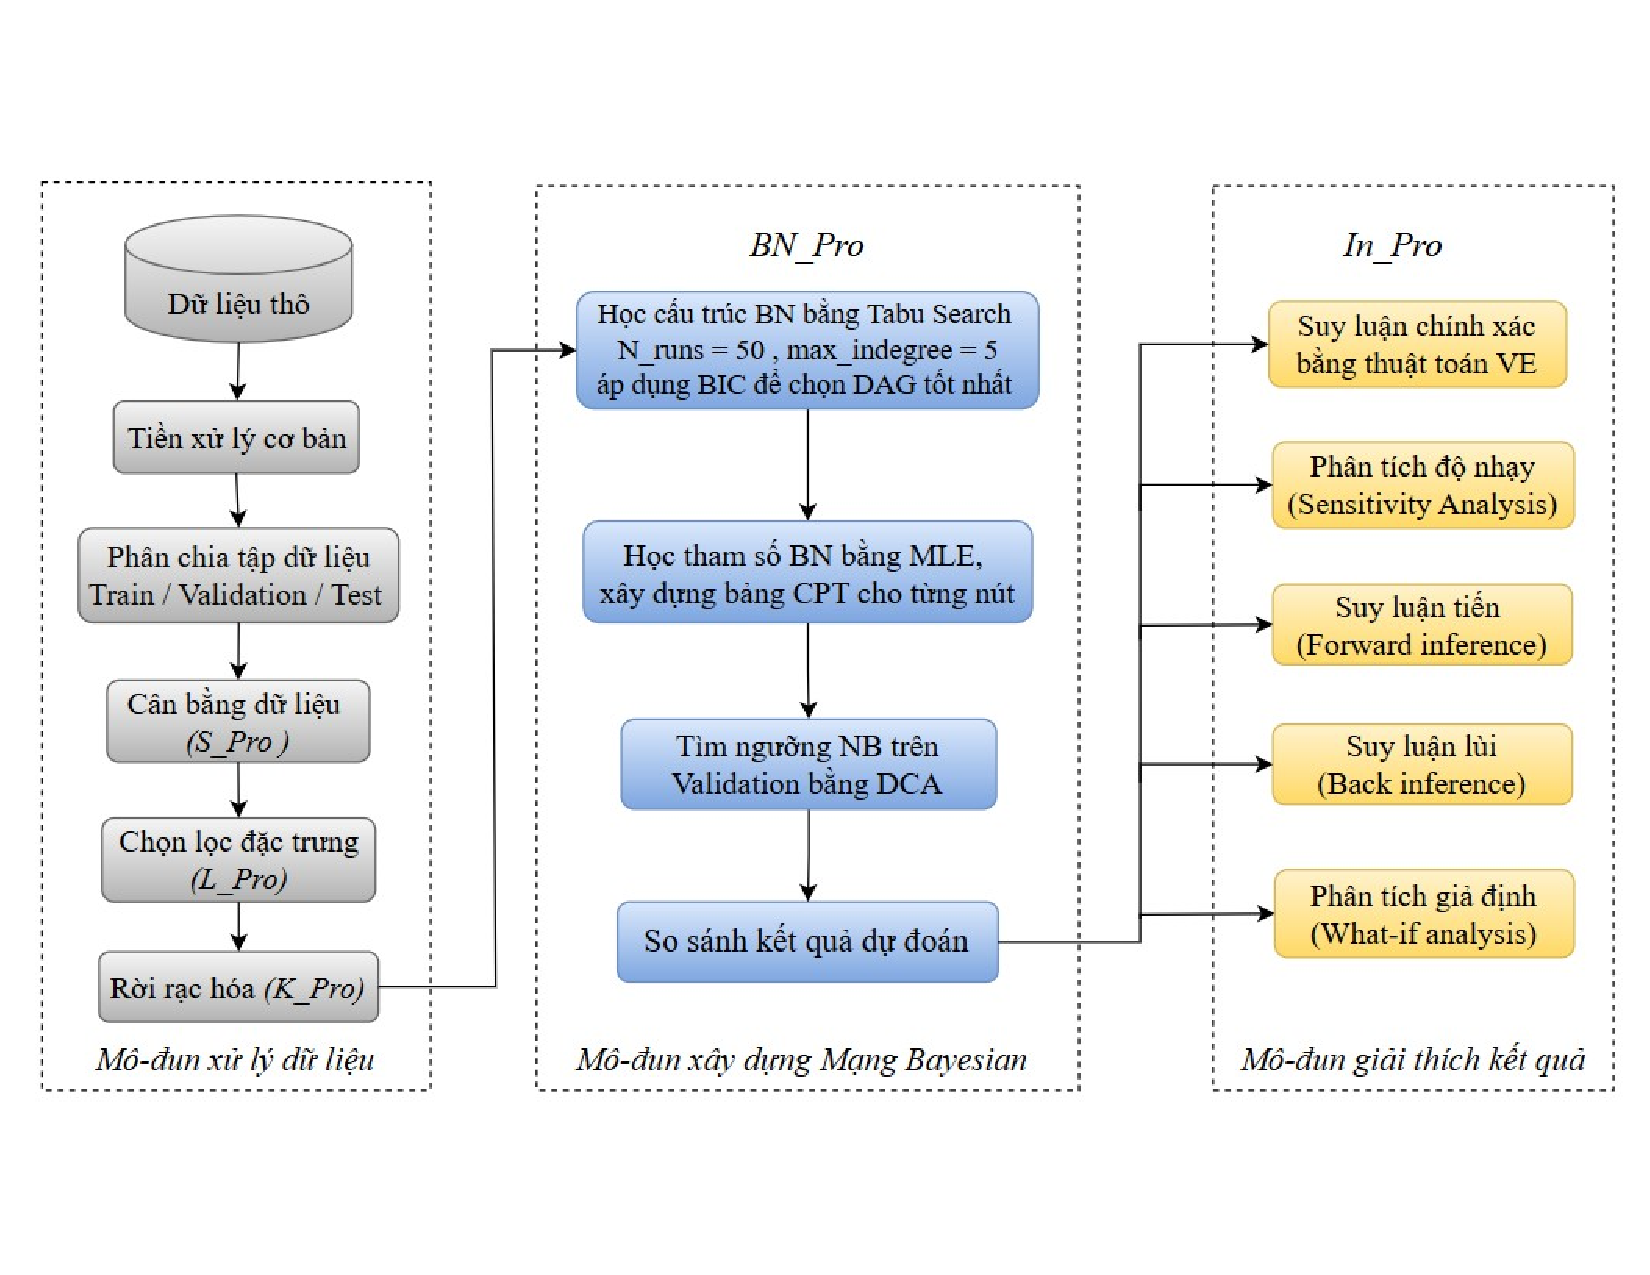
\includegraphics[width=1.05\textwidth,
    trim=0.5cm 2cm 0cm 3cm,
    clip]{image/frame.pdf}
    \caption{Framework of the proposed model.}
    \label{fig:framework}
\end{figure}
\FloatBarrier

\subsection{Data Processing Procedure}
\subsubsection{Data Balancing with SMOTE (S\_Pro)}
\noindent
In the credit risk prediction problem, the training dataset often exhibits severe class imbalance, with the number of default profiles (the minority class) considerably smaller than that of ordinary profiles (the majority class) (Table \ref{tab:dataset_summary}, Figure \ref{fig:class_imbalance}). Without intervention, machine learning algorithms tend to be biased towards the majority class, resulting in a distorted decision boundary and a severe reduction in the ability to identify genuine risk. To remedy this, the present study applies the Synthetic Minority Over-sampling Technique (SMOTE) in order to rebalance the class distribution before the data enters the Bayesian network structure learning procedure.
SMOTE operates by synthesising new minority samples rather than directly duplicating existing observations, thereby avoiding local overfitting \cite{chawla2002smote}. Specifically, for each minority sample $x_i$, the algorithm identifies the $k$ nearest neighbours in the feature space according to Euclidean distance, then randomly interpolates along the line segment joining $x_i$ to a randomly chosen neighbour $x_{nn}$ in order to create a new synthetic sample $x_{\text{new}}$ according to the formula:
\begin{equation}
    \label{eq:3.1}
    x_{\text{new}} = x_i + \lambda \cdot (x_{nn} - x_i), \quad \lambda \sim \mathcal{U}(0, 1)
\end{equation}
where $\lambda$ is a random value sampled uniformly from the interval $[0, 1]$. This process is repeated until the number of samples in the minority class is balanced with that of the majority class. The algorithm is presented as follows:

\vspace{0.5em}
\begin{algorithm}
\caption{Pseudocode of the SMOTE algorithm}
\vspace{0.5em}
\textbf{Input:} Minority sample set $X_{min}$, number of neighbours $k$, synthesis ratio $N$.

\vspace{0.5cm}
\textbf{Output:} Synthetic sample set $X_{syn}$.
\begin{tcolorbox}
\begin{algorithmic}[1]
    \State $X_{syn} \gets \emptyset$
    \For{each $x_i \in X_{min}$}
        \State Compute the $k$ nearest neighbours of $x_i$ in $X_{min}$ according to Euclidean distance
        \For{$n = 1$ to $N$}
            \State Randomly select $x_{nn}$ from the set of $k$ neighbours
            \State Sample $\lambda \sim \mathcal{U}(0, 1)$
            \State $x_{new} \gets x_i + \lambda \cdot (x_{nn} - x_i)$
            \State $X_{syn} \gets X_{syn} \cup \{x_{new}\}$
        \EndFor
    \EndFor
    \State \textbf{return} $X_{syn}$
\end{algorithmic}
\end{tcolorbox}
\end{algorithm}

The key point of the interpolation mechanism is that the synthetic samples created lie on the line segment joining two real samples in the feature space, and therefore always fall within a neighbourhood of genuine data density. This ensures that new samples are not generated in regions of space far removed from the original distribution, a common drawback of synthesis methods based on random noise. As a result, the decision boundary between the two classes is expanded and smoothed more naturally, helping the model to learn the discriminative characteristics of the minority class rather than merely memorising repeated samples.

\subsubsection{Feature Selection Using Lasso Regression (L\_Pro)}
\label{sec: 3.1.2}
\noindent
After the data balancing stage, the input feature space often contains many variables with low contribution or high mutual correlation, causing information redundancy and increasing the computational cost of the Bayesian network structure learning process — which is already an NP-hard problem. The feature selection step therefore plays an important role in reducing the dimensionality of the variable space while still preserving the discriminative power of the model.
This study applies Logistic regression with L1 regularisation (commonly referred to as Lasso regression) as the principal feature selection mechanism. Mathematically, Lasso adds to the objective function a penalty term proportional to the sum of the absolute values of the coefficients, forcing the coefficients of certain variables exactly to $0$ when the improvement in model fit from including a variable is not sufficient to offset its penalty in increasing the number of probability parameters to be estimated, thereby performing automatic feature selection within the parameter estimation process itself \cite{tibshirani1996lasso}. The corresponding optimisation problem is written as:

\vspace{1em}
\begin{equation}
    \hat{\beta} = \arg\min_{\beta} \left[ -\ell(\beta; \mathbf{X}, \mathbf{y}) + \frac{1}{C} \sum_{j=1}^{p} |\beta_j| \right],
\end{equation}
\noindent
where,
\begin{itemize}
    \item $\hat{\beta}$: The optimal set of coefficients (weights) to be estimated for the model.
    \item $\ell(\beta; \mathbf{X}, \mathbf{y})$: The log-likelihood function of the logistic model with respect to the feature matrix $\mathbf{X}$ and the vector of actual labels $\mathbf{y}$. 
    \begin{equation}
        \ell(\beta; \mathbf{X}, \mathbf{y}) = \sum_{i=1}^{n} \Big[ y_i \log p_i + (1 - y_i) \log (1 - p_i) \Big], \qquad p_i = \frac{1}{1 + e^{-\boldsymbol{\beta}^\top \mathbf{x}_i}}
    \end{equation}
    \item $\beta_j$: The weight coefficient corresponding to the $j$-th feature in the data.
    \item $p$: The total number of input features.
    \item $C$: The inverse of the penalty strength ($C > 0$), used to control the degree of regularisation of the model:
    \begin{itemize}
        \item \textit{When $C$ is small:} The strong penalty forces many coefficients $\beta_j$ decisively to $0$; specifically, a variable is eliminated when the improvement it brings to the log-likelihood function is smaller than the penalty that $L_1$ regularisation imposes on its coefficient, that is, when the marginal contribution of the variable is not sufficient to justify its retention in the model.
        \item \textit{When $C$ is large:} The penalty is weak, and the objective function tends towards the form of ordinary logistic regression without constraints.
    \end{itemize}
    \item $\sum_{j=1}^{p} |\beta_j|$: The L1 regularisation term (L1 norm), measuring the sum of the absolute values of the coefficients.
\end{itemize}

\subsubsection{Data Discretisation Using K-means (K\_Pro)}
\label{sec: 3.1.3}
\noindent
Bayesian networks require the input variables to be in discrete form so that conditional probability tables can be constructed through frequency statistics. When the data contains continuous variables, computing conditional probabilities directly over a continuous value domain is computationally infeasible and also leads to severe data sparsity in the cells of the CPT \cite{koller2009probabilistic}\cite{friedman1996discretizing}. The discretisation step is therefore a prerequisite for ensuring the validity of the network parameter learning process.

This study uses the K-means algorithm as its principal discretisation mechanism \cite{liu2024credit}. To understand the reason for this choice, we consider the differences between three common discretisation strategies. The equal-width method divides the entire value domain into $k$ intervals of equal width, regardless of the actual density of the data distribution. As a consequence, the bins in the tail regions of financial data distributions, which are typically strongly skewed, will contain very few observations, leading to unreliable estimates of conditional probability in the CPT. The equal-frequency method overcomes the density problem by ensuring that each bin contains approximately the same number of observations, but it may sever the natural clusters in the data when bin boundaries are placed arbitrarily according to quantiles. K-means, by contrast, divides the value domain on the basis of the actual geometric density structure, seeking bin boundaries such that the observations within the same bin are as similar to one another as possible. This is particularly meaningful for Bayesian networks, since more homogeneous bins produce CPT cells that more accurately reflect the true data-generating mechanism.

With $k$ bins determined in advance, K-means seeks a set of cluster centroids $\{\mu_1, \mu_2, \dots, \mu_k\}$ that minimises the total within-cluster sum of squared distances \cite{macqueen1967methods}:
\begin{equation}
    \label{eq: 3.3}
    \min_{\{S_i\}} \sum_{i=1}^{k} \sum_{x \in S_i} (x - \mu_i)^2,
\end{equation}

\noindent
where:
\begin{itemize}
    \item $k$: The total number of clusters (the number of bins) defined in advance.
    \item $S_i$: The set of data points (observations) assigned to the $i$-th cluster.
    \item $x$: A particular data point with a continuous value belonging to cluster $S_i$.
    \item $\mu_i$: The centroid of the $i$-th cluster, usually the mean value of all points $x$ lying within that cluster.
    \item $(x - \mu_i)^2$: The squared distance from the data point $x$ to its corresponding cluster centroid $\mu_i$.
\end{itemize}

In the centroid update step, the centroid of each cluster is recomputed as the arithmetic mean of all the points belonging to that cluster. This iterative process is guaranteed to converge because the objective function is non-negative and decreases monotonically after each iteration. The assignment step does not increase the total sum of squared distances, and the centroid update step likewise does not increase the value of the objective function, since the arithmetic mean is the minimiser of the sum of squared distances within a cluster. Each observation is then assigned the bin label corresponding to the index of the nearest cluster, converting the continuous value into a discrete ordinal variable $\{0, 1, \dots, k-1\}$ suited to the input requirements of the Bayesian network. The pseudocode of the algorithm is presented as follows:

\vspace{0.5em}
\begin{algorithm}[H]
\caption{Pseudocode of the K-means algorithm for discretisation}
\label{alg:kmeans_discretization}

\vspace{0.5em}
\textbf{Input:} Dataset $X$, number of bins $k$.

\vspace{0.5cm}

\textbf{Output:} Bin label $b(x) \in \{0, 1, \dots, k-1\}$ for each observation.

\begin{tcolorbox}
\begin{algorithmic}[1]
    \State Initialise $k$ cluster centroids $\{\mu_1, \mu_2, \dots, \mu_k\}$ randomly from $X$
    \Repeat
        \State \textbf{Assignment step:} $S_i \gets \{x \in X : |x - \mu_i| \leq |x - \mu_j|, \forall j \neq i\}$
        \State \textbf{Centroid update step:} $\mu_i \gets \frac{1}{|S_i|} \sum_{x \in S_i} x$
    \Until{the cluster centroids no longer change}
    \State Assign the bin label $b(x) \gets \arg\min_i |x - \mu_i|$ for each $x \in X$
    \State \textbf{return} $\{b(x)\}$
\end{algorithmic}
\end{tcolorbox}

\end{algorithm}

\subsection{Building the Bayesian Network (BN\_Pro)}
\noindent
Unlike black-box machine learning models such as Random Forest, XGBoost or Deep Neural Networks, which focus solely on optimising a predictive loss function, the Bayesian network aims to model the structure of probabilistic dependence among variables by establishing a qualitative structure through the concept of a directed acyclic graph, thereby allowing the mechanism by which credit risk is formed to be clearly described and probabilistic inference to be performed across the entire system \cite{pearl2009causality}, \cite{koller2009probabilistic}, \cite{darwiche2009modeling}.
A DAG is defined mathematically as a graph pair $G = (V, E)$, in which $V$ is the set of vertices representing the random variables in the credit model, and $E$ is the set of directed edges expressing the relationships of direct dependence between pairs of variables. The acyclicity property plays a foundational role, ensuring that if one starts from any node and moves along the direction of the arrows, there never exists a closed path in the system returning to the initial node. In the credit risk prediction problem, this property completely eliminates causal loops that are illogical in economic terms, while also establishing a clear structural ordering among the influencing factors, for example from demographic characteristics and financial history to repayment behaviour and finally to the state of default (Liu et al., 2024) \cite{liu2024credit}.
Applying Bayesian networks to credit risk prediction requires an extremely rigorous model construction procedure that transforms raw financial datasets into a system of causal knowledge capable of mathematical inference. According to Liu et al. (2024) \cite{liu2024credit}, the procedure for building the BN\_Pro model for the credit default prediction problem comprises three core stages: structure learning, estimation of the parameter space, and deployment of the probabilistic inference algorithm. These are three architectural layers tightly linked to one another. The structure learning stage aims to discover the dependency relationships among the variables in the data; the parameter learning stage quantifies the degree of that dependence through conditional probabilities; and the inference stage uses all the knowledge that has been learned to compute the probability of the target event occurring, such as the likelihood that a customer defaults (Default = 1). The organic combination of these three stages fundamentally resolves the barrier of computational complexity that always exists in multidimensional data spaces, while maximising the explanatory capacity of the model in the face of complex credit-granting decisions.
The learning process of a Bayesian network is not merely the optimisation of a predictive function as in Logistic Regression or Gradient Boosting, but the construction of a complete probabilistic model for the entire data system. This forms the foundation for interpretability, sensitivity analysis, counterfactual analysis and causal inference in modern financial research \cite{pearl2009causality}, \cite{liu2024credit}, \cite{peters2017elements}.


\subsubsection{Network Structure Learning}
\noindent
The process begins with determining the network structure, which the academic community has established as an NP-hard problem owing to the exponential explosion of the space of Directed Acyclic Graphs as the number of feature variables increases \cite{koller2009probabilistic}, \cite{jensen2007bayesian} . To overcome this computational barrier, instead of using exhaustive search methods over the entire space, which are infeasible in terms of resources, the structure learning process gives priority to heuristic search algorithms for approximating the globally optimal solution. Within the framework of this study, the Tabu Search algorithm proposed by Glover (1986) \cite{koller2009probabilistic} is deployed as a breakthrough local search tool, combined with the Bayesian information criterion in order to shape a causal network that both fits the data closely and remains structurally parsimonious \cite{liu2024credit}.

The essence of the Tabu Search algorithm is that it fundamentally overcomes the fatal weakness of ordinary hill climbing algorithms, namely becoming trapped at local optima. The algorithm operates by continuously traversing neighbouring graphs through spatial transformations such as adding an edge, deleting an edge or reversing the direction of an arrow. The core difference is the mechanism of maintaining a Tabu list that acts as a short-term memory; when a network structure or a transformation operation has just been evaluated, it is placed on this list and forbidden from being repeated for a certain number of iterations \cite{spirtes2000causation}. This enforcement mechanism prevents the algorithm from returning to previous moves, compelling the system to cross the valleys of the descending function in order to escape the local optimum trap and explore new regions of the structure space, thereby approaching the globally optimal structure \cite{liu2024credit}.

To evaluate the quality of each neighbouring structure during the traversal, the BIC score function is integrated as the ultimate objective function \cite{koller2009probabilistic}. The BIC score acts as a balancing mechanism, resolving the strict trade-off between the goodness of fit of the model (measured by the residual sum of squares or the Likelihood function) and the complexity of the model (measured by the number of free parameters) \cite{liu2024credit}. By imposing a logarithmic penalty on the network size and the number of samples, the BIC criterion effectively prevents overfitting and eliminates edges that cause an unnecessary explosion of parameters.

\begin{equation}
    BIC = \log P(D|\hat{\theta},G) - \frac{\log N}{2}\cdot k,
\end{equation}

\noindent
where:

\begin{itemize}
    \item \(D\): the training data.
    \item \(G\): the DAG structure.
    \item \(\hat{\theta}\): the optimal parameter set of the network.
    \item \(\log P(D|\hat{\theta},G)\): the Log-Likelihood, assessing the ability of the DAG to explain the data 
    \item \(N\): the number of samples.
    \item \(k\): the number of parameters to be estimated.
\end{itemize}
with $\frac{\log N}{2}\cdot k$ being the penalty coefficient for model complexity.

\vspace{1em}
This entire discovery process is placed within a meta-loop of 50 independent network initialisations and training runs in order to eliminate the risk of bias due to the initial starting point, ensuring that the final causal structure reflects the mechanism generating credit risk as faithfully and robustly as possible \cite{liu2024credit}. 

\begin{equation}
G^* = \arg\max_{r=1,...,50} BIC_r,
\end{equation}
where:

\begin{itemize}
    \item $G^*$: the optimal DAG structure selected.
    \item $r = 1,...,50$: the index of the models/DAG structures tested.
    \item $BIC_r$: the BIC score of the $r$-th model.
\end{itemize}

\vspace{1em}
\noindent

The construction and adjustment process is described in Algorithm \ref{alg:tabu_bic}.

\vspace{0.5em}
\begin{algorithm}[h]
\caption{Pseudocode of the BIC-based Tabu Search algorithm}
\label{alg:tabu_bic}
\vspace{0.5em}
\textbf{Initialisation:} A discrete Bayesian network in DAG form. 
Generate a random initial DAG as the current solution. 
Set the current best solution = the current solution = the DAG. 
Initialise the Tabu list and the BIC score.

\vspace{0.5cm}

\textbf{Output:} Return the Bayesian network structure with the highest BIC score.

\begin{tcolorbox}
\begin{algorithmic}[1]
\While{(the stopping criterion has not been met)}
    \State Generate feasible neighbouring network structures.
    \For{(each feasible neighbouring solution $N$)}
        \If{$N$ is not on the Tabu list}
            \State Compute the evaluation index $Q(N)$ of the neighbouring solution $N$ using the BIC score.
            \If{$Q(N) > Q$(the current optimal solution)}
                \State Update the current solution $= N$.
            \EndIf
        \EndIf
    \EndFor
    \State Select the neighbouring solution with the largest $Q(N)$ as the new current solution.
    \State Add the current solution to the Tabu list.
    \State Decrease the Tabu memory of the solutions already in the Tabu list by one unit.
\EndWhile

\State Repeat the Tabu Search algorithm several times with different initial DAGs.
\State Return the DAG with the highest BIC score.
\end{algorithmic}
\end{tcolorbox}
\end{algorithm}
\FloatBarrier

\subsubsection{Parameter Estimation}
\noindent
After the structure learning process has been completed and the directed acyclic graph determined, the Bayesian network has so far only represented the relationships of probabilistic dependence among the variables in the form of a graph structure. The DAG by itself, however, is not sufficient for performing probabilistic inference or predicting credit risk. For the Bayesian network to become a complete probabilistic model, as soon as the DAG skeleton has been firmly established, the system enters the parameter learning stage in order to quantify the causal space \cite{darwiche2009modeling}. The central task is to determine the Conditional Probability Tables for each network node, thereby delineating the degree of statistical dependence among the financial variables \cite{jensen2007bayesian}. This process operates on the basis of Maximum Likelihood Estimation (MLE), a canonical mathematical foundation that allows the observed frequencies from the historical dataset to be transformed directly into predictive probability distributions \cite{liu2024credit}.

According to the Bayesian network theory presented by Pearl \cite{pearl2009causality} and by Koller and Friedman \cite{koller2009probabilistic}, each edge in the DAG reflects only the existence of a relationship of probabilistic dependence between two variables, while the strength and quantitative nature of that relationship is encoded through the probability parameters in the CPT. Hence, if structure learning answers the question ``which variable influences which'', parameter learning answers the question ``how great the influence is'' \cite{pearl2009causality}, \cite{koller2009probabilistic}. 

Consider a Bayesian network comprising a set of $n$ random variables: \textbf{\textit{X}} = $(X_1,X_2,\ldots,X_n)$ with a known DAG structure.
According to the probability decomposition rule of Bayesian networks \cite{pearl2009causality}, \cite{koller2009probabilistic}, \cite{darwiche2009modeling}:
\begin{equation}
    P(X_1,X_2,...,X_n) = \prod_{i=1}^{n} P(X_i \mid Pa(X_i)),
\end{equation}


\noindent
where:

\begin{itemize}
    \item $X_i$ is the $i$-th variable in the network;
    \item$Pa(X_i)$ denotes the set of direct parent nodes of $X_i$;
    \item$P(X_i|Pa(X_i))$ is the probability of the variable $X_i$ given the states of its parent variables in the DAG.
\end{itemize}

\vspace{1em}
The expression above shows that the joint probability distribution of the entire system is decomposed into a product of local probability distributions.

In the credit risk prediction problem, this means that a customer's probability of default is not modelled directly by a single global function, but is derived from the combination of many conditional probabilities among the financial variables, credit behaviour, borrowing history and the target variable Default \cite{liu2024credit}, \cite{masmoudi2019credit}, \cite{leong2016credit}.

\vspace{1em}
\noindent
\textbf{Conditional Probability Table}

\noindent
Suppose the variable $X_i$ has $s_i$ different states.
Its parent set $Pa(X_i)$ has $q_i$ value configurations.
The parameter set to be learned is then:
$$\theta= \{ \theta_{ijk} | i = 1,\dots, n; j = 1,\dots, q; k = 1, \dots, s_i \}$$
with:
\begin{equation}
    \theta_{ijk} = P(X_i=k|Pa(X_i)=j),
\end{equation}

\noindent
where:

\begin{itemize}
    \item $i$: the variable under consideration.
    \item$j$: the $j$-th configuration of the parent set.
    \item $k$: the $k$-th state of the variable.
\end{itemize}

\vspace{1em}
According to Jensen and Nielsen \cite{jensen2007bayesian}, each row in the CPT must satisfy the normalisation constraint:
$$\sum_{k=1}^{s_i} \theta_{ijk} = 1$$
for all:
$$j=1,\ldots,q_i$$
This ensures that the total probability of all possible states of a variable always equals 1.

\vspace{1em}
\noindent
\textbf{The Likelihood Function}

\noindent
Analytically, the algorithm seeks the optimal parameter set such that the likelihood function attains its maximum value. In order to handle the enormous computational load, the algorithm converts the likelihood function into logarithmic form (the log-likelihood), turning complex products of simultaneous probabilities into a series of linear additions \cite{koller2009probabilistic}, \cite{liu2024credit}. By scanning the entire dataset, counting the number of samples satisfying the joint condition between the current node and its parent set, and applying the method of Lagrange multipliers to resolve the mathematical constraints, the system fills in the CPT with precisely the optimal probability percentages \cite{liu2024credit}. The resulting parameter grid not only describes the structure of the training data but also becomes the core quantitative knowledge base for every subsequent inference query \cite{darwiche2009modeling}, \cite{liu2024credit}. 

\vspace{1em}
\noindent
Suppose the training dataset:
$$D={d_1,d_2,\ldots,d_m}$$
consists of $m$ independent observations.

\vspace{1em}
According to Koller and Friedman \cite{koller2009probabilistic}, the likelihood function is defined as:
\begin{equation}
    L(\theta|D) = P(D|\theta) = \prod_{l=1}^{m} P(d_l|\theta),
\end{equation}
where:
\begin{itemize}
    \item $L(\theta|D)$: the likelihood function, representing the probability of observing the data $D$ given the parameters $\theta$.
    \item $D$: the training dataset.
    \item $\theta$: the parameter set of the Bayesian network.
    \item $P(d_l|\theta)$: the probability of the $l$-th data sample given the parameter set $\theta$.
    \item $m$: the total number of data samples in the training set.
\end{itemize}

    
\vspace{1em}
\noindent
The objective of MLE is to find the parameter set:
$$\theta^* = \arg\max_{\theta} L(\theta|D)$$
that is, the parameter set that makes the observed data most probable.

\vspace{1em}

Because the likelihood function is a product of a great many small probabilities, it is prone to arithmetic underflow. Studies on Bayesian networks therefore all switch to the log-likelihood \cite{koller2009probabilistic}, \cite{darwiche2009modeling}, \cite{liu2024credit}.

\vspace{1em}
Let $m_{ijk}$ denote the number of samples satisfying: $X_i=k$ and $Pa(X_i)=j$ 

Then:
\begin{equation}
\begin{aligned}
\label{eq: log}
\ell(\theta|D) 
&= \log L(\theta|D) \\
&= \log \prod_{l=1}^{m} P(d_l|\theta) \\
&= \sum_{i=1}^{n} \sum_{j=1}^{q_i} \sum_{k=1}^{s_i}
m_{ijk} \log(\theta_{ijk}),
\end{aligned}
\end{equation}
where:
\begin{itemize}
    \item $\ell(\theta|D)$: the log-likelihood function of the Bayesian network with parameter set $\theta$ and data $D$.
    \item $n$: the number of variables in the Bayesian network.
    \item $q_i$: the number of states of the parent set of the variable $X_i$.
    \item $s_i$: the number of states of the variable $X_i$.
    \item $m_{ijk}$: the number of times the variable $X_i$ is observed in state $k$ while the parent set is in state $j$.
    \item $\theta_{ijk}$: the conditional probability of the variable $X_i$ being in state $k$ given the $j$-th parent state.
\end{itemize}

\vspace{1em}
In order to maximise the log-likelihood function $\ell(\theta|D)$ in formula \ref{eq: log}, the probability normalisation constraint must be satisfied for each node $X_i$ and each combination of parent states $j$:
\begin{equation}
    \sum_{k=1}^{s_i} \theta_{ijk} = 1, \quad \forall i \in \{1,\ldots,n\},\ \forall j \in \{1,\ldots,q_i\}
\end{equation}

\vspace{1em}
This is an optimisation problem with equality constraints, and the method of Lagrange multipliers is therefore applied. The Lagrangian function is constructed as follows:
\begin{equation}
    \mathcal{L}(\theta, \lambda) = \sum_{i=1}^{n}\sum_{j=1}^{q_i}\sum_{k=1}^{s_i} m_{ijk}\log(\theta_{ijk})\ +\ \sum_{i=1}^{n}\sum_{j=1}^{q_i} \lambda_{ij}\!\left(1 - \sum_{k=1}^{s_i}\theta_{ijk}\right)
\end{equation}
where $\lambda_{ij}$ is the Lagrange multiplier corresponding to the constraint at node $X_i$ and the $j$-th combination of parent states.

\vspace{1em}
\noindent
Taking the partial derivative of $\mathcal{L}$ with respect to $\theta_{ijk}$ and setting it equal to 0:

\begin{equation}
    \frac{\partial \mathcal{L}}{\partial \theta_{ijk}} = \frac{m_{ijk}}{\theta_{ijk}} - \lambda_{ij} = 0 \implies \theta_{ijk} = \frac{m_{ijk}}{\lambda_{ij}}
\end{equation}

\vspace{1em}
\noindent
Substituting into the normalisation constraint to determine $\lambda_{ij}$:

\begin{equation}
    \sum_{k=1}^{s_i}\theta_{ijk} = \sum_{k=1}^{s_i}\frac{m_{ijk}}{\lambda_{ij}} = \frac{1}{\lambda_{ij}}\sum_{k=1}^{s_i}m_{ijk} = 1 \implies \lambda_{ij} = \sum_{k=1}^{s_i}m_{ijk} = m_{ij\cdot}
\end{equation}
where $m_ij = \sum_{k=1}^{s_i}m_{ijk}$ is the total number of observations whose parent set is in state $j$, regardless of the state of $X_i$.

\vspace{1em}
\noindent
Substituting back, the explicit solution of the MLE problem is:
\begin{equation}
    \boxed{\hat{\theta}_{ijk} = \frac{m_{ijk}}{m_{ij\cdot}}}
\end{equation}

\vspace{1em}
This solution has a clear intuitive meaning: the optimal conditional probability of $X_i$ being in state $k$ when the parent set is in state $j$ is precisely the relative frequency observed in the training data. This is the mathematical basis on which the MLE class in the pgmpy library fills in the values of the CPT: instead of iterative optimisation, it need only count the frequency of occurrence of each combination of states $(X_i = k, Pa(X_i) = j)$ in the training set and compute the ratio. This is the central formula of the entire parameter learning process in Bayesian networks \cite{koller2009probabilistic}, \cite{liu2024credit}.

\subsubsection{Initialising the Inference Mechanism and Markov Blanket Analysis}
\noindent
Immediately after the complete Bayesian network has been built, an exact inference engine based on the variable elimination algorithm is initialised in conjunction with the model, serving as the sole interface through which all probabilistic queries in the In\_Pro phase will pass. Before exploiting the inference mechanism for prediction and explanation purposes, a preliminary sanity check is carried out: the unconditional prior probability P(target = 1) is queried directly from the Variable Elimination engine and compared against the empirical prior probability prior\_default computed directly from the frequencies in the training data. Agreement between these two values (with a discrepancy smaller than a conventionally agreed tolerance threshold) is a necessary (though not sufficient) condition for asserting that the graph structure and the learned Conditional Probability Distributions (CPD) correctly encode the latent dependency relationships in the original data, since if inference over the network cannot exactly reproduce the marginal distribution of the target variable that was used to learn those parameters, there is a high likelihood of an error in constructing the graph or in estimating the CPT.
In parallel with this validation step, an important structural analysis is performed, namely determining the Markov Blanket set of the target variable, denoted MB(target), which is formally defined as the union of three subsets: the set of direct parents (Parents), the set of direct children (Children), and the set of parents of the children (Parents of Children, also known as the set of ``spouses''):
$$MB(target) = Parents(target) \cup  Children(target) \cup Parents(Children(target))$$
According to Pearl's definition \cite{pearl2009causality} within the framework of Bayesian networks, the core theoretical significance of the Markov Blanket is the property of conditional independence separation: once the states of all the variables in MB(target) are known, the target variable becomes conditionally independent of every remaining variable in the network that does not belong to the Markov Blanket 
\[
\textit{target} \perp (\textit{all other variables}) \mid \textit{MB(target)}
\]
\vspace{1em}
The direct practical consequence of this property is that the Markov Blanket is precisely the minimal and sufficient feature set required to predict the target variable accurately within the framework of the learned model: adding any variable outside MB(target) to the evidence set of an inference query will not contribute any additional marginal information for estimating P(target | evidence), because the entire influence of those variables (if any) has already been transmitted and fully ``absorbed'' through the intermediate variables belonging to the Markov Blanket. This is the theoretical basis for the study's use of the Markov Blanket as a tool for structural explanation, running in parallel with the specific probabilistic inference analyses in the In\_Pro phase.

\subsection{Interpretation of Results (In\_Pro)}
\noindent
Successfully constructing a Bayesian network does not stop at prediction; the graph structure must also be fully exploited in order to explain the mechanism by which risk is formed. The Interpretation Process (In\_Pro) block serves as a bridge between the computational power of machine learning and the human need to understand root causes. This stage operates mainly on two core foundations: the mechanism of multidimensional probabilistic inference and the technique of sensitivity analysis combined with mutual information.

\subsubsection{Exact Inference Using the Variable Elimination Algorithm}
\noindent
Once the Bayesian network has been completed in terms of both its qualitative geometric structure and its quantitative parameter system, the next core problem is to exploit the model in order to produce scientific judgements when real-world information appears. This process is called probabilistic inference, in which the system updates the probability distribution of one or a group of target variables given the specific known states of another group of observed variables, which serve as empirical evidence (Liu et al., 2024) \cite{liu2024credit}. Within the scope of rigorous mathematical methods, exact inference is the approach that computes posterior probability values that are absolute and analytically precise, rather than using stochastic approximation techniques that carry uncertainty. The results of exact inference ensure that every risk decision made rests on a purely mathematical logical foundation, unaffected by simulation error.

In the context of credit risk prediction research, the ultimate goal is not to determine the probability of each individual variable but to infer the probability of a customer defaulting given an observed set of specific credit information. This is equivalent to computing the posterior probability:

\begin{equation}
    P(Default=1 \mid X_1=x_1, X_2=x_2, ..., X_m=x_m)
\end{equation}

\noindent
in which the set of observed variables serves as the evidence, while the variable Default serves as the query variable \cite{liu2024credit}.

\vspace{1em}
According to Pearl (2009) \cite{pearl2009causality}, the inference process in a BN is precisely the process of belief updating when new information appears. Mathematically, this is carried out through Bayes' theorem combined with the probability decomposition structure of the network.This form of decomposition is the foundation that allows a BN to handle complex inference problems by exploiting conditional independence. This is precisely the important advantage that makes BNs suitable for the credit risk assessment problem, in which factors such as income, credit history, financial behaviour and loan status are mutually dependent \cite{pearl2009causality}, \cite{koller2009probabilistic}, \cite{darwiche2009modeling}. 

Although the probabilistic representation becomes more efficient, performing exact inference on a Bayesian network remains a problem of very high computational complexity. Cooper (1990) \cite{cooper1990computational} proved that the problem of exact probabilistic inference on a BN belongs to the NP-hard class. This means that the computational cost may grow exponentially as the number of variables or the density of connections in the network increases. For this reason, the choice of an appropriate inference algorithm plays a decisive role in the practical applicability of Bayesian networks in large-scale credit risk prediction systems. 

In the study by Liu et al. \cite{liu2024credit}, as well as in the model \ proposed in this thesis, the Variable Elimination (VE) algorithm is chosen as the exact inference mechanism for computing a customer's probability of default from the learned Bayesian network structure. 

\vspace{1em}
\noindent
\textbf{The Variable Elimination Algorithm}

\noindent
VE is one of the classic exact inference algorithms for Bayesian networks, developed on the ideas of non-sequential dynamic programming and the technique of decomposing the inference problem into local operations on probabilistic factors \cite{darwiche2009modeling}, \cite{jensen2007bayesian}, \cite{dechter1999bucket}.

The core idea of the algorithm is to avoid computing the entire joint probability distribution of the network directly. Instead, VE takes advantage of the graph structure and the relationships of conditional independence to carry out probability additions and multiplications in an optimal order so as to reduce the number of operations that must be performed \cite{darwiche2009modeling}.

\vspace{1em}
Suppose we need to compute:
$$P(Y|E=e)$$ 
where $Y$ is the query variable and $E$ is the set of evidence variables. By the definition of posterior probability:

\begin{equation}
    P(Y \mid E = e) = \frac{P(Y, E = e)}{P(E = e)} = \frac{\sum_{z} P(Y, E = e, Z = z)}{\sum_{y, z} P(Y = y, E = e, Z = z)},
\end{equation}

\noindent
where:
\begin{itemize}
    \item $P(Y \mid E = e)$: The posterior probability of the target state variable $Y$ (for example, the likelihood of default) after the evidence set $E = e$ has been observed.
    \item $Y$, $y$: The target variable to be queried and its specific state.
    \item $E$, $e$: The set of evidence variables in the Bayesian network and the specific values actually recorded (for example, the customer has a low income or a history of late payment).
    \item $Z$, $z$: The set of intermediate variables belonging neither to the target group $Y$ nor to the evidence group $E$, and their state space.
    \item $\sum_z$: The marginalisation summation over the entire state space of $Z$, in order to eliminate the influence of these intermediate variables from the query result.
    \item $\sum_{y, z}$: The summation over the entire state space of both $Y$ and $Z$ in order to compute the marginal probability $P(E = e)$ in the denominator, which acts as a normalising constant ensuring that the total probability equals $1$.


\item $P(E=e)$ is the probability of the evidence occurring
\item $P(Y,E=e)$ is the joint probability of the query variable and the evidence. 
\end{itemize}

\vspace{1em}
If the summation is performed directly over the entire state space of $Z$ $(O(k^n))$, where $k$ is the average number of states per variable and $n$ is the number of hidden variables, the computational cost will grow exponentially. VE resolves this problem by changing the order of the multiplication and summation operations:

$$\sum_Z \prod_i f_i$$
\noindent
into a sequence of local operations:

$$\sum_{Z_k} \left( f_1 \cdot f_2 \cdots f_m \right)$$
\noindent
such that only one intermediate variable $Z_k$ is removed from the system at a time.

It is precisely this interchange of the order of multiplication and summation that allows VE to reduce inference complexity considerably compared with the brute-force method \cite{darwiche2009modeling}, \cite{dechter1999bucket}, \cite{murphy2012machine}. Algorithm \ref{alg:magia_VE} below is the pseudocode of the VE algorithm.

\vspace{1em}
\begin{algorithm}
    \caption{Pseudocode of the variable elimination inference algorithm}
\vspace{0.5em}
\label{alg:magia_VE}

\textbf{Input:} Bayesian network $BN$.

\vspace{0.2cm}

\textbf{Output:} Return the posterior probability $P(Y|E=e)$.

\vspace{0.2cm}
\begin{tcolorbox}
\begin{algorithmic}[1]
\State Initialise the VE inference engine with $BN$.

\vspace{0.1cm}
\State Set the query variable $Y$ and the evidence $E=e$.

\vspace{0.1cm}
\State Extract the factors $F$ from $BN$.

\vspace{0.1cm}
\While{hidden variables remain}

\vspace{0.1cm}
    \State Select a variable $X$ from the elimination order $\rho$.

\vspace{0.1cm}
    \State Multiply the factors containing $X$.

\vspace{0.1cm}
    \State Eliminate $X$ by summation.

\vspace{0.1cm}
\EndWhile

\vspace{0.1cm}
\State Combine the remaining factors to obtain $h(Y)$.

\vspace{0.1cm}
\State Return $P(Y|E=e) = h(Y) \text{/} \sum_Y h(Y)$.

\end{algorithmic}
\end{tcolorbox}
\end{algorithm}

A Bayesian network represents the joint distribution as a product of local CPDs: $P(X_1,...,X_1)$. From the computational standpoint of the VE algorithm, each of these CPDs is regarded as a factor, that is, a function defined over a subset of variables, mapping each combination of states of those variables to a non-negative probability value. A factor $f(A, B, C)$ need not be a normalised probability distribution; it need only be a table of values capable of taking part in multiplication and aggregation operations.

\begin{enumerate}
    \vspace{1em}
    \item \textbf{Factor multiplication}

    When two factors share one or more variables, for instance $f_1(A, B)$ and $f_1(B, C)$, factor multiplication produces a new factor over the union of the participating variables:
    \begin{equation}
        f(A, B, C) = f_1(A, B) \times f_2(B, C)
    \end{equation}
    where, for each specific combination of states of $(A, B, C)$, the value of the resulting factor equals the product of the corresponding values of the two component factors at the shared state combination of the variable $B$. This operation is the basic computational building block that allows the local joint distribution to be reconstructed gradually from the initial discrete CPDs, without explicitly constructing the entire joint distribution table over all variables.


    \vspace{1em}
    \item \textbf{Variable elimination}

    Instead of computing the summation directly over the entire state space of the hidden variables, the VE algorithm marginalises the hidden variables one at a time, immediately after multiplying the factors related to that variable, according to the distributive law of addition over multiplication:
    
    \begin{equation}
        \sum_{\text{hidden}} \prod_i f_i \Rightarrow \sum_{\{Z_1\}} \left(\sum_{\{Z_2\}} \left( ... \left( f_1 \times f_2 \times ... \times f_m \right) ... \right)\right)
    \end{equation}
    
    \hspace{0.5cm} Specifically, for each variable $X_k$ to be eliminated in the predetermined elimination order $\rho=(X_1,X_2,\ldots,X_k)$, the algorithm groups together all the existing factors that still contain $X_k$, multiplies them into an intermediate factor, then sums out $X_k$ from this intermediate factor to obtain a new factor no longer containing $X_k$, and replaces the old factors with this new factor in the set of factors being processed. The process is repeated until all hidden variables have been eliminated, leaving factors containing only the query variable $Y$, which are multiplied together to obtain $h(Y)$ and finally normalised into a valid posterior distribution:
    \begin{equation} 
        P(Y | E = e) = \frac{h(Y)}{\sum_Y h(Y)}
    \end{equation}

\end{enumerate}

The complexity advantage of VE over brute-force enumeration lies in the fact that the aggregation order is arranged so that each aggregation operation acts only on small local factors rather than on the global joint distribution table. However, the computational complexity of VE depends directly on the treewidth of the graph corresponding to a particular elimination order, and finding the elimination order that minimises treewidth is itself an NP-hard problem. In practice, pgmpy applies heuristics for selecting the elimination order based on the smallest node degree (the min-degree heuristic) in order to approximate an efficient elimination order, and with the credit network structure used in this research, the computational cost of VE remains within feasible limits for the repeated queries required by sensitivity and what-if analysis.

\subsubsection{Probabilistic Inference in Bayesian Networks}
\vspace{1em}
\noindent
\textbf{Forward Inference}

\noindent
The core essence of the interpretive power of Bayesian networks lies in their capacity for probabilistic inference, which operates on the firm foundation of Bayes' theorem. Unlike closed algorithms that establish only a one-directional mapping from input to output, the Bayesian network uses the organic relationship between the joint probability distribution function and the conditional probability distribution functions to carry out multidirectional inference. In terms of graph representation, each node in the network stands for a random variable, while the directed edges connecting the nodes depict directly the relationships of conditional dependence among these variables. Accompanying that geometric structure, each node possesses a conditional probability distribution table, which describes quantitatively the shift in the probability distribution at that node when the values of its dependent variables (the parent variables) change. This decomposition allows the system to represent the joint probability of the entire variable space $X = \{X_1, X_2, \dots, X_n\}$ through a product of local probabilities according to the formula:

\begin{equation}
    P(X_1, \dots, X_n) = \prod_{i=1}^n P(X_i | Pa(X_i))
\end{equation}

On the basis of that architecture, the forward inference mechanism is defined as the process of computing the posterior probability distribution of a target variable given evidence provided by one or more feature variables $P(Y|E=e)$. 

Considered in the experimental context of the credit-granting problem, by learning from the historical dataset of individuals who have previously taken out loans, the model can establish the structure and the intrinsic conditional probability distributions among the feature nodes, for example computing the probability that an individual has a borrowing need and a risk of default under the constraining conditions of their current income level and their past credit rating score \cite{liu2024credit}. As soon as the system receives an entirely new application for a personal credit limit, the forward inference process is immediately activated. The empirical values of that individual's income and credit score are assigned directly into the network as evidence variables. Through the Bayesian inference engine, the system propagates probabilities along the directed edges of the graph, thereby automatically computing and outputting the posterior probability distribution expressing that individual's borrowing need as well as their potential default rate \cite{murphy2012machine}. This process is not a mere approximation of a function but a circulation and updating of belief entirely grounded in the laws of statistical probability.

\vspace{1em}
\noindent
\textbf{Backward Inference}

\noindent
In parallel with forward inference, the Bayesian network also provides a superior mathematical basis for backward inference, otherwise known as diagnostic reasoning. In this direction of inference, the algorithm computes the posterior probability distribution of one or more feature variables (causes) once the specific state of one or more target variables (effects) has been observed \cite{pearl2009causality}. For instance, when the system records a profile that has genuinely fallen into the state of default, backward inference will diagnose and reconstruct the probability of occurrence of the income levels or credit behaviours that led to that outcome. 

\vspace{1em}
\noindent
Suppose:
\begin{itemize}
    \item $Y$: the target variable, which in this study is Default.
    \item $X$: the feature variable to be inferred (for example, Income, CreditScore, etc.).
\end{itemize}

\vspace{1em}
Given that the customer has defaulted ($Y=1$), the posterior probability of the feature variable is determined by:
\begin{equation}
    P(X|Y=1) = \frac{P(Y=1|X)\,P(X)} {P(Y=1)},
\end{equation}

\noindent
where:
\begin{itemize}
    \item $P(X|Y=1)$: the posterior probability of the variable $X$ given that the customer has defaulted.
    \item $P(Y=1|X)$: the probability that the customer defaults given the value of $X$.
    \item $P(X)$: the prior probability of the variable $X$.
    \item $P(Y=1)$): the prior probability of the target variable, acting as a normalising constant.
\end{itemize}

\vspace{1em}
The ability to combine forward inference (to predict the future) and backward inference (to diagnose causes) seamlessly is precisely the theoretical reason why Bayesian networks have become the gold standard in artificial intelligence systems specialising in probabilistic inference and financial decision-making \cite{darwiche2009modeling}, \cite{liu2024credit}. By continuously adding and updating new evidence in the observation space, the graph continuously refines the probability distribution curves, thereby sharpening the precision and accuracy of credit judgements in subsequent cycles.


\subsubsection{Sensitivity Analysis Method}
\label{sec: 3.3.3}
\noindent
In order to measure quantitatively and to isolate the mechanism of influence within the network structure, sensitivity analysis is deployed as a key posterior evaluation tool. Within the Bayesian network ecosystem, sensitivity analysis is usually decomposed into two specialised lines of reasoning: structural sensitivity analysis and parameter sensitivity analysis \cite{kamal2021sensitivity}, \cite{rohmer2020sensitivity}. On the structural analysis side, the degree of influence on the target variables is assessed by directly adjusting the network architecture: researchers actively intervene in the geometric skeleton of the DAG through operations such as grafting on, or eliminating, nodes and links (edges). After each structural transformation, the algorithm recomputes the posterior probability distribution and compares it with the original network in order to measure the discrepancy; the larger the discrepancy, the more it demonstrates the acute sensitivity of the target to that structural change. Parameter sensitivity analysis, by contrast, focuses on preserving the graph architecture while actively intervening in the intrinsic parameters of the network, specifically the values inside the conditional probability distribution table.

Within the scope of this study, the focus of the analysis is placed entirely on parameter sensitivity analysis, in order to exploit to the fullest the local interpretability of the model with respect to credit scenarios. By applying the control variable method thoroughly, the researcher can actively change the value of a single input variable (for example, the borrower's income level) while freezing all the remaining variables. By repeating this trial many times and recording the continuous change in the probability of default, the model quantifies precisely the magnitude of that feature's influence on overall risk. The variable that produces the largest shift in probability is precisely the variable with the highest sensitivity. 

\vspace{1em}
Suppose the input variable $X$ changes from the value $x_1$ to $x_2$; the degree of change in the posterior probability is determined by:

\begin{equation}
    \Delta P=P(Y=1|X=x_2)-P(Y=1|X=x_1),
\end{equation}

\noindent
where:
\begin{itemize}
    \item $\Delta P$ is the change in the probability of default;
    \item $X$ is the variable being analysed;
    \item $x_1,x_2$ are two states of the variable.

\end{itemize}

\noindent
The larger $|\Delta P|$ is, the more sensitive that variable is for the predictive model.

\vspace{1em}
Successfully locating the nodes of maximum sensitivity not only provides management with a solid basis for operating the system safely and stably, but also guides purposeful risk intervention measures. At the same time, the results of this process can be used to optimise the model directly by readjusting the weights of the variables or by deciding to collect additional new variables with higher explanatory potential \cite{lin2020behavioral}, \cite{bishop2006pattern} .

To provide a powerful quantitative mathematical basis for determining sensitivity and the degree of association, the study applies the theory of mutual information. In a Bayesian network, mutual information quantitatively expresses the degree of correlation and information sharing between two random variables. Measuring the mutual information between network nodes helps to indicate whether the conditional probability distributions between them are mutually constrained \cite{murphy2012machine}, \cite{cover2006elements}. 

The mathematical formula expressing the mutual information between the feature variable $X$ and the target variable $Y$ is defined as the integral (or the sum, for discrete variables) of the joint distribution function multiplied by the logarithm of the ratio between the joint distribution and the product of the marginal distributions:

\begin{equation}
    I(X;Y) = \sum_{x \in X} \sum_{y \in Y} P(x,y) \log \left( \frac{P(x,y)}{P(x)P(y)} \right)
\end{equation}

\vspace{1em}
If the mutual information between two nodes equals $I(X;Y) = 0$, this is absolute mathematical proof that the two nodes are entirely conditionally independent in the context of the neighbouring nodes already determined. By analysing the mutual information spectrum of the target node, analysts can distil and rank precisely the degree of association between the input feature nodes and the danger of default, thereby eliminating noisy features and establishing an optimal inference space that is extremely convincing for the predictive results.


\subsection{Evaluation of Predictive Performance}

\subsubsection{Receiver Operating Characteristic Curve}
\noindent
In the binary classification problem, the Receiver Operating Characteristic curve (ROC), or ROC curve, is a graphical representation illustrating the performance of a binary classification system as its discrimination threshold is varied continuously over the entire range of possible values. The ROC curve is created by plotting the ratio of true positives to the total number of actual positive samples (TPR) against the ratio of false positives to the total number of actual negative samples (FPR) at different threshold settings [60]. In the context of credit risk prediction, positive is usually taken by convention to be the case of a customer defaulting, while negative is the case of a customer repaying on time (non-default).

The classification model takes as input the customer's financial features and produces a risk score $s$, expressing the degree to which a default event is likely to occur. Based on a classification threshold $c \in (0,1)$, customers are classified into two groups:
\begin{equation}
    \hat{Y}= \begin{cases} 1, & \text{if } s\geq c\\ 0, & \text{if } s<c \end{cases},
\end{equation}
where:
\begin{itemize}
    \item $\hat{Y}=1$: the customer is predicted by the model to be at risk of default (Default).
    \item $\hat{Y}=0$: the customer is predicted by the model not to default (Non-default).
    \item $c$: the classification threshold chosen to convert the continuous risk score into a binary classification decision.

\end{itemize}

\vspace{1em}
After comparing the model's predictions with the customers' actual states, we obtain a Confusion Matrix comprising four cases:

\begin{itemize}
    \item $TP$ (True Positive): the number of customers who actually default and are correctly predicted by the model as defaulting.
    \item $TN$ (True Negative): the number of customers who do not actually default and are correctly predicted by the model as non-defaulting.
    \item $FP$ (False Positive): the number of customers who do not actually default but are incorrectly predicted by the model as defaulting.
    \item $FN$ (False Negative): the number of customers who actually default but are incorrectly predicted by the model as non-defaulting.
\end{itemize}

\vspace{1em}
From the quantities above, the two important components constituting the ROC curve are determined to be sensitivity and the false positive rate (FPR).

\vspace{1em}
Sensitivity, or the rate of correctly detecting defaulting customers, is denoted $Se(c)$ or $TPR(c)$:

\begin{equation}
    TPR(c)=Se(c)=\frac{TP(c)}{TP(c)+FN(c)}
\end{equation}

This quantity reflects the model's ability to identify customers with high credit risk accurately. The larger the value of $TPR(c)$, the fewer potentially defaulting customers the model overlooks.

\vspace{1em}
Conversely, specificity expresses the ability to identify the group of non-defaulting customers accurately:

\begin{equation}
    Sp(c)=\frac{TN(c)}{TN(c)+FP(c)}
\end{equation}

From specificity, the rate at which good customers are wrongly predicted to be risky customers is determined by:

\begin{equation}
    FPR(c)=1-Sp(c)
\end{equation}

or:
\begin{equation}
    FPR(c)=\frac{FP(c)}{FP(c)+TN(c)},
\end{equation}
where:
\begin{itemize}
    \item $FPR(c)$ expresses the proportion of customers who do not default but are misclassified by the model as defaulting at the threshold $c$.
    \item $Sp(c)$ reflects the model's ability to correctly rule out non-risky cases.
\end{itemize}

\vspace{1.5em}

Suppose the risk score output by the model has the corresponding probability density functions:

$$f(s|Y=1) \quad \text{and} \quad f(s|Y=0),$$
where:
\begin{itemize}
    \item $f(s|Y=1)$: the probability density function of the risk score for the group of customers who actually default.
    \item $f(s|Y=0)$: the probability density function of the risk score for the group of customers who do not actually default.
    \item $s$: the risk score predicted by the model.
    
\end{itemize}


\vspace{1.5em}
With a classification threshold $c$, a customer is predicted to default if: $s\geq c$. The probability that the model correctly detects a defaulting customer is then expressed as:
\begin{equation}
    TPR(c)=Se(c)=P(s\geq c|Y=1)
\end{equation}

or:

\begin{equation}
    TPR(c)=\int_{c}^{\infty}f(s|Y=1)ds
\end{equation}

\vspace{1em}
\noindent
Similarly, the probability that the model misclassifies a non-defaulting customer as a defaulting one is determined as:

\begin{equation}
    FPR(c)=P(s\geq c|Y=0)
\end{equation}
or:

\begin{equation}
    FPR(c)=\int_{c}^{\infty}f(s|Y=0)ds
\end{equation}

\noindent
Thus, for each different threshold value $c$, the model produces a pair of values:

$$(FPR(c),TPR(c))$$

\vspace{1em}
When $c$ is allowed to vary continuously over the entire range of the score $s$, the set of these points forms a curve in the two-dimensional space $[0,1]\times[0,1]$. The resulting curve is precisely the ROC curve.

\vspace{1em}
Unlike overall accuracy, the ROC curve does not depend on the prevalence of the default class in the dataset — a key property, since real-world credit data is usually severely imbalanced \cite{chawla2002smote}, with defaulting customers typically accounting for only a small fraction of the whole. At the same time, the ROC curve allows researchers to evaluate classification performance across the entire range of decision thresholds, thereby helping credit institutions to adjust their credit-granting threshold flexibly according to their specific risk appetite, for instance prioritising the minimisation of missed defaulting customers (increasing $Se$) or prioritising the minimisation of wrongful rejection of good customers (increasing $Sp$).


\subsubsection{Area Under the ROC Curve}
\noindent
While the ROC curve provides a comprehensive visual representation of classification performance across all thresholds, it does not directly yield a single aggregate figure for quantitative comparison between models. To address this limitation, the Area Under the ROC Curve (AUC) is introduced as a single scalar measure reflecting the entire discriminative capacity of a classifier across all possible thresholds. The area under a receiver operating characteristic curve, abbreviated AUC, is a single scalar numerical value measuring the overall performance of a binary classifier \cite{hanley1982meaning}.

The landmark theoretical contribution to the statistical interpretation of AUC belongs to Hanley and McNeil (1982) \cite{hanley1982meaning}, who proved an important result: AUC is equivalent in value to the Mann--Whitney U test (also known as the Wilcoxon rank-sum statistic). Given a set of positive samples P and negative samples N, AUC equals the proportion of all (positive, negative) pairs in which the classifier assigns a higher score to the positive sample. This interpretation gives AUC a highly intuitive probabilistic meaning of great practical value: AUC is precisely the probability that the test result of a subject chosen at random from the diseased group (or the defaulting group) exceeds that of a subject chosen at random from the non-diseased group (or the non-defaulting group) \cite{bamber1975area}. Applied to the credit risk problem, this means that AUC reflects the probability that the model assigns a higher risk score to a randomly chosen defaulting customer than to a randomly chosen non-defaulting customer, making it a criterion for evaluating the ranking ability of the model independently of the choice of any particular threshold.

\vspace{1em}
AUC is defined as the integral of the $TPR$ function with respect to $FPR$ over the entire domain $[0,1]$:

\begin{equation}
    AUC = \int_{0}^{1} TPR\big(FPR^{-1}(x)\big) dx = P(S_1 > S_0),
\end{equation}
where:
\begin{itemize}
    \item $S_1$: the risk score assigned by the model to a customer chosen at random from the defaulting group;
    \item $S_0$: the risk score assigned by the model to a customer chosen at random from the non-defaulting group, independent of $S_1$;
    \item $P(S_1 > S_0)$: the probability that a defaulting customer receives a higher score than a non-defaulting customer.
\end{itemize}


\vspace{1em}
In practice, with finite data, AUC is usually estimated through the formula equivalent to the Mann--Whitney U statistic that Hanley and McNeil showed to be:

\begin{equation}
    \widehat{AUC} = \frac{U_1}{n_1 \cdot n_0} = \frac{1}{n_1 n_0}\sum_{i=1}^{n_1}\sum_{j=1}^{n_0} \psi(s_i, s_j)
\end{equation}
with:
\begin{equation}
    \psi(s_i, s_j) = \begin{cases} 1, & \text{if } s_i > s_j \\ 0{.}5, & \text{if } s_i = s_j \\ 0, & \text{if } s_i < s_j, \end{cases}
\end{equation}

\noindent
where:
\begin{itemize}
    \item $n_1$: the number of defaulting customers (positive samples) in the test dataset;
    \item $n_0$: the number of non-defaulting customers (negative samples) in the test dataset;
    \item $s_i$: the risk score of the $i$-th defaulting customer $(i = 1, \dots, n_1)$;
    \item $s_j$: the risk score of the $j$-th non-defaulting customer $(j = 1, \dots, n_0)$;
    \item $U_1$: the Mann--Whitney U statistic computed over the positive--negative sample pairs;
    \item $\psi(s_i, s_j)$: the indicator function comparing each pair of scores, taking the value 1 if the pair is correctly ordered (a concordant pair), 0.5 in the case of a tie, and 0 if incorrectly ordered (a discordant pair).
\end{itemize}

\vspace{1em}
When the data is represented as discrete points on the empirical ROC curve $(FPR_k, TPR_k)_{k=0}^{m}$, AUC can also be computed approximately by the trapezoidal rule:

\begin{equation}
    \widehat{AUC} = \sum_{k=1}^{m} \frac{(TPR_k + TPR_{k-1})}{2} \times (FPR_k - FPR_{k-1})
\end{equation}

\vspace{1em}
Here $m$ is the number of discrete threshold points used to construct the empirical ROC curve. The AUC value lies within the interval [$0.5,1.0$], where the minimum value represents the performance of a random classifier and the maximum value corresponds to a perfect classifier \cite{hanley1982meaning}. Regarding estimation accuracy, Hanley and McNeil (1982) also proposed a closed-form analytical formula for computing the variance of AUC based on the AUC value, the number of positive samples and the number of negative samples, although bootstrap resampling is usually preferred in modern experimental work because it provides better coverage for extreme AUC values \cite{hanley1982meaning}.

In research, AUC serves as the most common benchmark criterion for comparing performance between different models, from classical statistical models such as linear discriminant analysis \cite{altman1968financial} and logistic regression \cite{ohlson1980financial} to modern machine learning models such as random forests \cite{breiman2001random}, support vector machines \cite{vapnik1998statistical}, \cite{shen2022credit} and ensemble methods \cite{breiman1996bagging}, \cite{friedman2001greedy}. Because AUC is independent of the choice of any particular threshold, it allows an objective assessment of the model's intrinsic discriminative capacity before the researcher must make a decision about the optimal classification threshold for practical deployment.

\subsubsection{Criteria for Finding the Optimal Classification Threshold}
\noindent
Although AUC provides a comprehensive measure of the model's discriminative capacity across the entire range of thresholds, in operational practice credit institutions are obliged to select a specific decision threshold $c$ in order to classify customers as granted credit or rejected/placed under risk monitoring. The choice of this threshold cannot be arbitrary but must rest on optimisation criteria with a clear theoretical basis, constructed directly from the geometry and statistics of the ROC curve; in this section we present the mathematical definitions of the methods for determining the optimal threshold that are most commonly used in research on diagnostic accuracy \cite{unal2017defining}. Below is a detailed analysis of the three criteria used in this study.

\begin{enumerate}[label=\alph*)]
    \vspace{1em}
    \item \textbf{The Youden Index Maximisation Criterion}

    The Youden index (Youden's J statistic, or Youden's index) was first introduced by the statistician William J. Youden \cite{youden1950index} in 1950, within the framework of studies aimed at improving the accuracy of medical diagnostic tests. Youden's $J$ statistic is a single number summarising the performance of a binary diagnostic test. It combines sensitivity and specificity into a single index, making it easy to compare tests and to find the optimal decision threshold on a continuous score. Geometrically, the Youden index is precisely the greatest vertical distance between the ROC curve and the reference diagonal (the chance line), that is, the greatest vertical distance between the ROC curve and the chance diagonal, and it is at the same time mathematically equivalent to the Kolmogorov--Smirnov distance statistic\footnote{The Kolmogorov--Smirnov distance statistic is the value measuring the greatest distance between two cumulative distribution functions} measuring the degree of separation between the two score distributions of the defaulting and non-defaulting groups \cite{schisterman2005optimal}.

    \hspace{0.5cm} An important theoretical advantage of the Youden index, which has led to its wide application in credit rating research, is its independence from the prevalence of the positive class in the population. Because it does not depend on the prevalence of the disease, Youden's $J$ index can be transferred between populations with different base rates, unlike predictive values \cite{youden1950index}. This property is particularly well suited to the credit risk prediction problem, where the actual default rate often varies considerably across customer segments, credit products, or stages of the economic cycle.

    \vspace{1em}
    \hspace{0.5cm} The Youden index at the threshold $c$ is defined as:
    \begin{equation}
        J(c) = Se(c) + Sp(c) - 1
    \end{equation}
    and the optimal threshold according to this criterion is determined by:
    \begin{equation}
        c_J = \underset{c \in \mathbb{R}}{\arg\max} J(c),
    \end{equation}
    where:
    \begin{itemize}
        \item $J(c)$: the Youden index at the classification threshold $c$;
        \item $Se(c)$: the sensitivity at the threshold $c$, that is, the proportion of defaulting customers correctly identified by the model;
        \item $Sp(c)$: the specificity at the threshold $c$, that is, the proportion of non-defaulting customers correctly identified by the model;
        \item $c_J$: the optimal classification threshold according to the Youden index maximisation criterion;
        \item $\arg\max_{c}$: the operator finding the value of $c$ that makes the function $J(c)$ attain its maximum over the entire real domain of the threshold.
    \end{itemize}
        \vspace{1em}
        \hspace{0.5cm} The index $J(c)$ takes values in the interval $[-1, 1]$, where $J = 0$ corresponds to a model with no discriminative ability whatsoever (the threshold lies on the reference diagonal of the ROC), while $J = 1$ corresponds to a perfect classification model with neither false positives nor false negatives A $J$ value of zero means that the test provides no useful information, while a value of one indicates perfect classification with no false positives or false negatives \cite{youden1950index}. Youden's $J$ index is one of the oldest and most widely used optimal-threshold frameworks, determining the threshold by maximising the sum of sensitivity and specificity across the different threshold points \cite{unal2017defining}.
        
        \hspace{0.5cm} However, an important theoretical limitation of the Youden criterion was pointed out by Smits (2010) \cite{smits2010note}: maximising $J(c)$ implicitly assumes a misclassification cost ratio equal to $1$ minus the prevalence of the positive class, an assumption that does not always accurately reflect the decision-maker's real priorities.

    
    \vspace{1em}
    \item \textbf{The Closest-to-(0,1) Criterion}

    Also known as the Euclidean distance criterion, formally introduced by Perkins and Schisterman in 2006  \cite{perkins2006inconsistency}, it is based on the geometric intuition that the most ideal operating point on the ROC curve is the point corresponding to a perfect classifier, that is, the point with coordinates $(FPR, TPR) = (0,1)$. Perkins and Schisterman introduced the closest-to-$(0,1)$ criterion, which selects the optimal threshold by minimising the distance of the points on the ROC curve to the perfect classification point $(0,1)$, where both sensitivity and specificity attain their maximum values. In essence this is a direct geometric rule: the optimal threshold is determined at the empirical operating point on the ROC curve with the shortest Euclidean distance to the ideal point $(0,1)$ \cite{ghosal2025impact}.

    \vspace{1em}
    \hspace{0.5cm} The Euclidean distance from the operating point at the threshold $c$ to the ideal point $(0,1)$ is computed as:
    \begin{equation}
        D(c) = \sqrt{\big(1 - Se(c)\big)^2 + \big(1 - Sp(c)\big)^2}
    \end{equation}
    and the optimal threshold according to this criterion is determined by:
    \begin{equation}
        c_{D} = \underset{c \in \mathbb{R}}{\arg\min} D(c)
    \end{equation}
    
    \hspace{0.5cm} This criterion is equivalent to simultaneously minimising the sum of the squares of $FNR (1-Se)$ and $FPR (1 - Sp)$; an estimator based on the smallest sum of squares of 1 minus sensitivity and 1 minus specificity is preferred when sensitivity and specificity are regarded as equally important. Compared with the Youden criterion, the closest-to-(0,1) criterion tends to react more sensitively to asymmetric deviations between the two types of classification error, since it applies a quadratic penalty to the deviation along each axis separately, instead of considering only a linear sum as the Youden index does.
    
    \vspace{1em}
    \item \textbf{The Symmetry Point Criterion}

    The Symmetry Point criterion (the Equal Sensitivity-Specificity Criterion, or the intersection point of the sensitivity and specificity curves) is based on the principle of determining the optimal classification threshold at the position where sensitivity and specificity attain balanced values. When the ROC curve has an area under the curve smaller than one, a trade-off always exists between the ability to correctly detect positive subjects (sensitivity) and the ability to correctly rule out negative subjects (specificity). The optimal threshold can therefore be determined by finding the value of $c$ such that the discrepancy between sensitivity and specificity is smallest.

    \hspace{0.5cm} This approach has a theoretical basis closely related to research on threshold selection when sensitivity and specificity are valued equally, a topic systematically examined in the study by Froud and Abel (2014) \cite{froud2014using} comparing methods for determining the minimally important change threshold in clinical outcome measurement Using ROC curves to select the threshold of minimally important change when sensitivity and specificity are valued equally. The core principle of this group of methods is that, when there is no basis for assigning different cost weights to the two types of classification error ($FP$ and $FN$), the balance point where the two indices $Se$ and $Sp$ are equal is regarded as the fairest and most neutral operating point.

    \vspace{1em}
    \hspace{0.5cm} The optimal symmetry threshold is determined as the solution $c$ of the equation:
    $$Se(c) = Sp(c)$$
    or equivalently, is determined by minimising the absolute deviation between these two quantities:
    \begin{equation}
        c_{S} = \underset{c \in \mathbb{R}}{\arg\min} \big|Se(c) - Sp(c)\big|
    \end{equation}


    \hspace{0.5cm} The threshold $c_{S}$ corresponds to the intersection between the empirical ROC curve and the auxiliary line $TPR+FPR=1$ in ROC space. This criterion has an important practical advantage in the prediction problem. It produces a balanced operating point at which the error rates between the two customer groups (those wrongly rejected and those wrongly granted credit) are equivalent as a percentage within each group, thereby helping credit institutions to maintain a consistent and transparent credit-granting policy that is not excessively biased towards either of the two types of risk (credit risk and the risk of losing customers/business opportunities). It should be noted, however, that the symmetry point criterion, like the Youden criterion, still implicitly assumes cost parity between the two types of classification error, and therefore needs to be applied with consideration for the specific risk management strategy of each financial institution, particularly given that credit data usually exhibits a high degree of class imbalance \cite{chawla2002smote}.


\end{enumerate}

\subsubsection{The Decision Curve Analysis Method}
\noindent
Decision Curve Analysis (DCA) was first formally introduced by Vickers and Elkin \cite{vickers2006decision} in 2006 in the journal \textit{Medical Decision Making}, with the aim of addressing an important gap remaining in traditional methods of evaluating predictive models. While accuracy measures such as sensitivity, specificity and the area under the receiver operating characteristic curve are essential for evaluating predictive models, they cannot capture the practical consequences of deploying such models in the real world. Specifically, measures such as AUC or the Youden index, although they reflect the intrinsic discriminative capacity of the model across the entire range of thresholds, entirely fail to quantify the practical value of a specific decision (for instance the decision to grant or refuse a loan) to the decision-maker, since they treat all classification thresholds as equally important, whereas in reality the consequences of a false positive and a false negative usually carry very different meanings and costs.

The theoretical foundation of DCA stems from formalising the relationship between the decision probability threshold $c$ and the exchange rate between the benefit of a $TP$ and the harm of a $FP$. In the context of credit risk prediction, the concept of the threshold $c$ has a practical interpretation as the minimum probability of default at which a credit institution decides to refuse credit (or to require additional risk mitigation measures such as raising the interest rate or requiring collateral). A low threshold $c$ reflects a prudent credit policy, in which the institution regards the harm of wrongly granting credit to a customer who will default (a false negative in the original logic, or correspondingly ``approve a bad loan'') as far more serious than the harm of wrongly rejecting a good customer; conversely, a high threshold $c$ reflects a credit expansion policy that prioritises maximising the number of loans disbursed and accepts a higher risk of default.

\vspace{1em}
The original formula for Net Benefit proposed by Vickers and Elkin (2006) \cite{vickers2006decision}, computed on a test dataset of $N$ observations, is expressed as follows; in the original paper, the net benefit is computed as:

\begin{equation}
    NB(c) = \frac{TP(c)}{N} - \frac{FP(c)}{N}\left(\frac{c}{1-c}\right),
\end{equation}
where:
\begin{itemize}
    \item $NB(c)$: the net benefit of the model at the decision probability threshold $c$;
    \item $TP(c)$: the number of customers who genuinely default and are correctly predicted by the model at the decision threshold $c$;
    \item $FP(c)$: the number of customers who genuinely do not default but are wrongly predicted by the model as going to default at the decision threshold $c$;
    \item $N$: the total number of observations (customers) in the test dataset;
    \item $\frac{c}{1-c}$: the odds ratio at the threshold $c$, acting as a weighting factor that converts the number of false positives into the same unit of harm as the number of true positives.
\end{itemize}

\vspace{1em}
The formula above is often expressed in an equivalent form in terms of sensitivity, specificity and prevalence, which is more convenient for linking it to the ROC framework presented in the previous sections \cite{vickers2019guide}:

\begin{equation}
    NB(c) = Se(c) \times \pi - \big(1 - Sp(c)\big) \times (1-\pi) \times \frac{c}{1-c}
\end{equation}

The formula above shows that DCA is not a method entirely separate from the ROC framework; rather, it uses the very structural components of the ROC curve ($Se$, $Sp$) as its input material, while adding two elements that ROC/AUC entirely ignore: the actual prevalence of the event ($\pi$) and the relative cost weighting between the two types of error (through the factor $c/(1-c)$) — moving beyond AUC: decision curve analysis to quantify the net benefit of risk prediction models \cite{sadatsafavi2021moving}.

\vspace{1em}
\noindent
\textbf{The Decision Curve and the Reference Lines}

\noindent
After computing $NB(c)$ at a range of different values of $c$ (usually spread evenly over a practically meaningful probability interval, for example from 0.01 to 0.5), plotting $NB(c)$ against $c$ forms the decision curve; plotting the net benefit against the threshold probability produces the decision curve \cite{vickers2006decision}. For the decision curve to have practical interpretive meaning, it is always presented together with two reference strategies serving as comparison standards:

\vspace{1em}
\begin{enumerate}
    \item \textit{Treat All}: assumes that every observation is classified as positive (in the credit context, equivalent to rejecting/monitoring every customer), regardless of the model score. The net benefit of this strategy is computed as:

    \begin{equation}
        NB_{\text{All}}(c) = \pi - (1-\pi)\times\frac{c}{1-c}
    \end{equation}

    \item \textit{Treat None}: assumes that every observation is classified as negative (no customer is rejected on the basis of the model), in which case $TP(c)=FP(c)=0$ and the net benefit is therefore always zero at every threshold; the treat-none strategy assumes that no observation receives the intervention, and by definition its net benefit is always zero across all thresholds:
    
    \begin{equation}
        NB_{\text{None}}(c) = 0 \quad \forall c \in (0,1),
    \end{equation}
    
    \vspace{1em}
    where:
    \begin{itemize}
        \item $NB_{\text{All}}(c) $: the net benefit of the treat-all strategy at the threshold $c$;
        \item $NB_{\text{None}}(c)$: the net benefit of the treat-none strategy at the threshold $c$ (always equal to 0);
        \item $\pi$: the prevalence of the positive class.
    \end{itemize}

\end{enumerate}

A predictive model is considered to have practical value at a specific threshold $c$ if and only if its decision curve lies above both of these reference lines at that threshold; the model provides genuine benefit only within the range of thresholds where its curve lies above both reference strategies. The intersection point of these two reference lines, which occurs precisely at $c = \pi$, carries important guiding significance for determining the range of practically meaningful thresholds to examine in a given study.

Although DCA was developed and popularised mainly in the field of medical statistics, where it has become a routinely recommended tool to supplement traditional measures of discrimination and calibration when evaluating clinical predictive models — decision curve analysis addresses this limitation by incorporating the concept of net benefit, allowing a more comprehensive assessment of a model's clinical usefulness \cite{vickers2006decision} — the underlying mathematical structure of the method is entirely transferable to the credit risk prediction problem, since both problems are essentially binary classification problems governed by a decision threshold with asymmetric costs between the two types of error.

Research on default prediction has long been well aware of the core problem that DCA seeks to resolve: the cost of wrongly rejecting a good customer, leading to lost business opportunity and lost interest revenue, and the cost of wrongly approving a customer who will default, leading to loss of principal, are entirely asymmetric and depend strongly on each institution's own risk management strategy — an evaluation that takes into account the financial consequences of false positives (rejecting good borrowers) and false negatives (approving risky borrowers). The DCA theoretical framework provides a more systematic and quantitatively rigorous approach to formalising this trade-off, going beyond reliance on the qualitative intuition of risk experts or on heuristic rules for making subjective decisions when assessing a user's credit risk.


The decision curve allows the researcher or the risk management department of a credit institution to answer an important practical question: ``at what level of default probability threshold does using the predictive model to make credit-granting decisions yield a higher net benefit than the two extreme strategies of approving all loan applications or rejecting all loan applications?'' This is of far greater practical significance than merely reporting a single AUC figure or Youden index, because it allows the entire range of thresholds at which the model genuinely creates added value to be illustrated visually, while also exposing cases in which a model with a high AUC but poor calibration — that is, where the predicted probabilities do not accurately reflect the actual frequency of default — may still be harmful (yielding a negative net benefit) over certain ranges of thresholds. This constitutes an important premise, warning researchers of the latent risk in evaluating complex machine learning models, where the problem of probability calibration is often overlooked when the researcher focuses solely on optimising AUC or classification accuracy.












\newpage
\section{Thực nghiệm và đánh giá}
\noindent
Chương này trình bày toàn bộ quá trình thực nghiệm của khung dự đoán rủi ro tín dụng dựa trên Causal Machine Learning, được triển khai và đánh giá trên ba bộ dữ liệu tín dụng thực tế với đặc điểm và quy mô khác nhau: Australian Credit Dataset, German Credit Dataset và Lending Club 2007–2014. Bên cạnh việc so sánh hiệu suất phân loại giữa mạng Bayes và các thuật toán máy học cơ sở, chương này còn trình bày chi tiết kết quả của từng giai đoạn trong đường ống xử lý dữ liệu, cấu trúc đồ thị nhân quả học được, cũng như các phân tích diễn giải mô hình thông qua suy luận tiến, suy luận lùi và phân tích kịch bản what-if.

\subsection{Dữ liệu thực nghiệm}
\noindent
Để đánh giá toàn diện hiệu quả của khung dự đoán rủi ro tín dụng dựa trên Causal Machine Learning, nghiên cứu này triển khai thực nghiệm trên ba bộ dữ liệu tín dụng thực tế với quy mô, nguồn gốc và đặc điểm cấu trúc khác nhau, bao gồm Australian Credit Dataset, German Credit Dataset và Lending Club 2007 - 2014. Mỗi bộ dữ liệu đại diện cho một bối cảnh thẩm định tín dụng riêng biệt, từ đó cho phép đánh giá khả năng tổng quát hóa của mô hình trên nhiều loại hình dữ liệu tài chính.

\subsubsection{Mô tả bộ dữ liệu}
Australian Credit Dataset được thu thập từ UCI Machine Learning Repository, phản ánh thông tin hồ sơ tín dụng cá nhân tại Úc với dữ liệu đã được ẩn danh hóa hoàn toàn. Bộ dữ liệu gồm 690 mẫu quan sát và 14 đặc trưng đầu vào sau khi loại bỏ cột mã bưu chính (ZipCode) do không mang giá trị phân biệt rủi ro. Trong số 14 đặc trưng còn lại, 5 biến mang bản chất liên tục gồm Age, Debt, YearsEmployed, CreditScore và Income; 8 biến còn lại là biến phân loại danh nghĩa gồm Gender, BankCustomer, EducationLevel, Ethnicity, CreditHistory, Employed, DriversLicense và Citizen. Phân phối nhãn mục tiêu tương đối cân bằng với 383 mẫu vỡ nợ (55.5\%) và 307 mẫu không vỡ nợ (44.5\%), không tồn tại giá trị khuyết. Bộ dữ liệu được chia theo tỷ lệ 60/40 cho tập huấn luyện và tập kiểm tra.

German Credit Dataset cũng được lấy từ UCI Machine Learning Repository, đại diện cho bài toán phân loại rủi ro tín dụng trong bối cảnh ngân hàng Đức. Bộ dữ liệu gồm 1,000 mẫu quan sát với 20 đặc trưng đầu vào. Trong đó, 3 biến liên tục là month\_duration, credit\_amount và age; 17 biến còn lại là biến phân loại bao gồm status\_account, credit\_history, purpose, status\_savings, years\_employment, status\_and\_sex, secondary\_obligor, collateral, other\_installment\_plans, housing, job, telephone, is\_foreign\_worker và một số biến phụ trợ khác. Nhãn mục tiêu được mã hóa lại từ định dạng chuỗi (``good'' $\rightarrow$ 0, ``bad'' $\rightarrow$ 1), với phân phối 700 mẫu tốt (70\%) và 300 mẫu xấu (30\%), thể hiện sự mất cân bằng lớp ở mức vừa phải. Bộ dữ liệu không có giá trị khuyết và được chia theo tỷ lệ 60/40.

Lending Club 2007-2014 là bộ dữ liệu cho vay ngang hàng quy mô lớn được thu thập từ nền tảng Lending Club, bao gồm 466.345 hồ sơ vay với 151 cột thông tin gốc. Do quy mô và độ phức tạp đặc thù của bộ dữ liệu này, quá trình tiền xử lý đòi hỏi nhiều bước làm sạch chuyên sâu hơn so với hai bộ dữ liệu còn lại. Trước tiên, biến mục tiêu được nhị phân hóa từ cột loan\_status: các trạng thái ``Fully Paid'', ``Current'' và ``Does not meet the credit policy. Status: Fully Paid'' được gán nhãn 0 (không vỡ nợ), trong khi các trạng thái ``Charged Off'', ``Late'', ``In Grace Period'' và ``Does not meet the credit policy. Status: Charged Off'' được gán nhãn 1 (vỡ nợ). Tiếp theo, các cột không mang thông tin thẩm định (id, url, mô tả văn bản) và các cột gây rò rỉ dữ liệu tương lai (total\_pymnt, recoveries, last\_pymnt\_amnt và các biến phản ánh kết quả sau khi giải ngân) bị loại bỏ hoàn toàn. Các cột có tỷ lệ giá trị khuyết vượt quá 50\% cũng bị loại. Trên không gian biến số còn lại, phân tích hệ số phóng đại phương sai (VIF) và lọc tương quan được áp dụng để xử lý đa cộng tuyến, đưa số lượng biến liên tục từ 36 xuống mức tối ưu trước khi đưa vào Lasso. Kết hợp với 10 biến phân loại gồm term, grade, emp\_length, verification\_status, home\_ownership, purpose, addr\_state, initial\_list\_status, hardship\_flag và debt\_settlement\_flag, không gian đặc trưng cuối cùng được xác định. Do giới hạn tài nguyên tính toán khi học cấu trúc mạng Bayes trên tập dữ liệu cực lớn, nghiên cứu lấy mẫu con có kiểm soát với 21,000 mẫu không vỡ nợ và 9,000 mẫu vỡ nợ, tạo thành tập làm việc gồm 30,000 quan sát với tỷ lệ mất cân bằng xấp xỉ 7:3, phản ánh gần đúng phân phối tự nhiên của dữ liệu gốc. Tập này sau đó được chia theo tỷ lệ 60/40 cho huấn luyện và kiểm tra.

Thông tin tổng hợp về ba bộ dữ liệu được trình bày trong Bảng \ref{tab:dataset_summary}.

\begin{table}[htbp]
    \centering
    \caption{Thông tin tổng hợp về các bộ dữ liệu thực nghiệm}
    \label{tab:dataset_summary}
    \renewcommand{\arraystretch}{1.3} % Tăng khoảng cách dòng để bảng thoáng hơn
    \begin{tabular}{|l|c|c|c|c|}
        \hline
        \textbf{Bộ dữ liệu} & \textbf{Số mẫu} & \textbf{Số đặc trưng} & \textbf{Không vỡ nợ} & \textbf{Vỡ nợ} \\ \hline
        Australian & 690 & 14 & 307 & 383 \\ \hline
        German & 1,000 & 20 & 700 & 300 \\ \hline
        Lending Club & 30,000 & 46 & 21,000 & 9,000 \\ \hline
    \end{tabular}
\end{table}

\subsubsection{Phân tích khám phá dữ liệu (EDA)}
\noindent
Trước khi tiến hành xây dựng mô hình, quá trình phân tích khám phá dữ liệu (EDA) được thực hiện trên cả ba bộ dữ liệu nhằm làm rõ đặc điểm phân phối, mức độ mất cân bằng lớp và cấu trúc tương quan giữa các đặc trưng. Kết quả phân tích này đồng thời cung cấp cơ sở thực nghiệm cho các quyết định thiết kế trong đường ống tiền xử lý dữ liệu ở các bước tiếp theo. 

\vspace{1em}
\noindent
\textbf{Mức độ mất cân bằng lớp}

\vspace{0.5em}
\begin{figure}[htbp]
    \centering
    % Hình 1: Australian
    \begin{subfigure}[b]{0.43\textwidth}
        \centering
        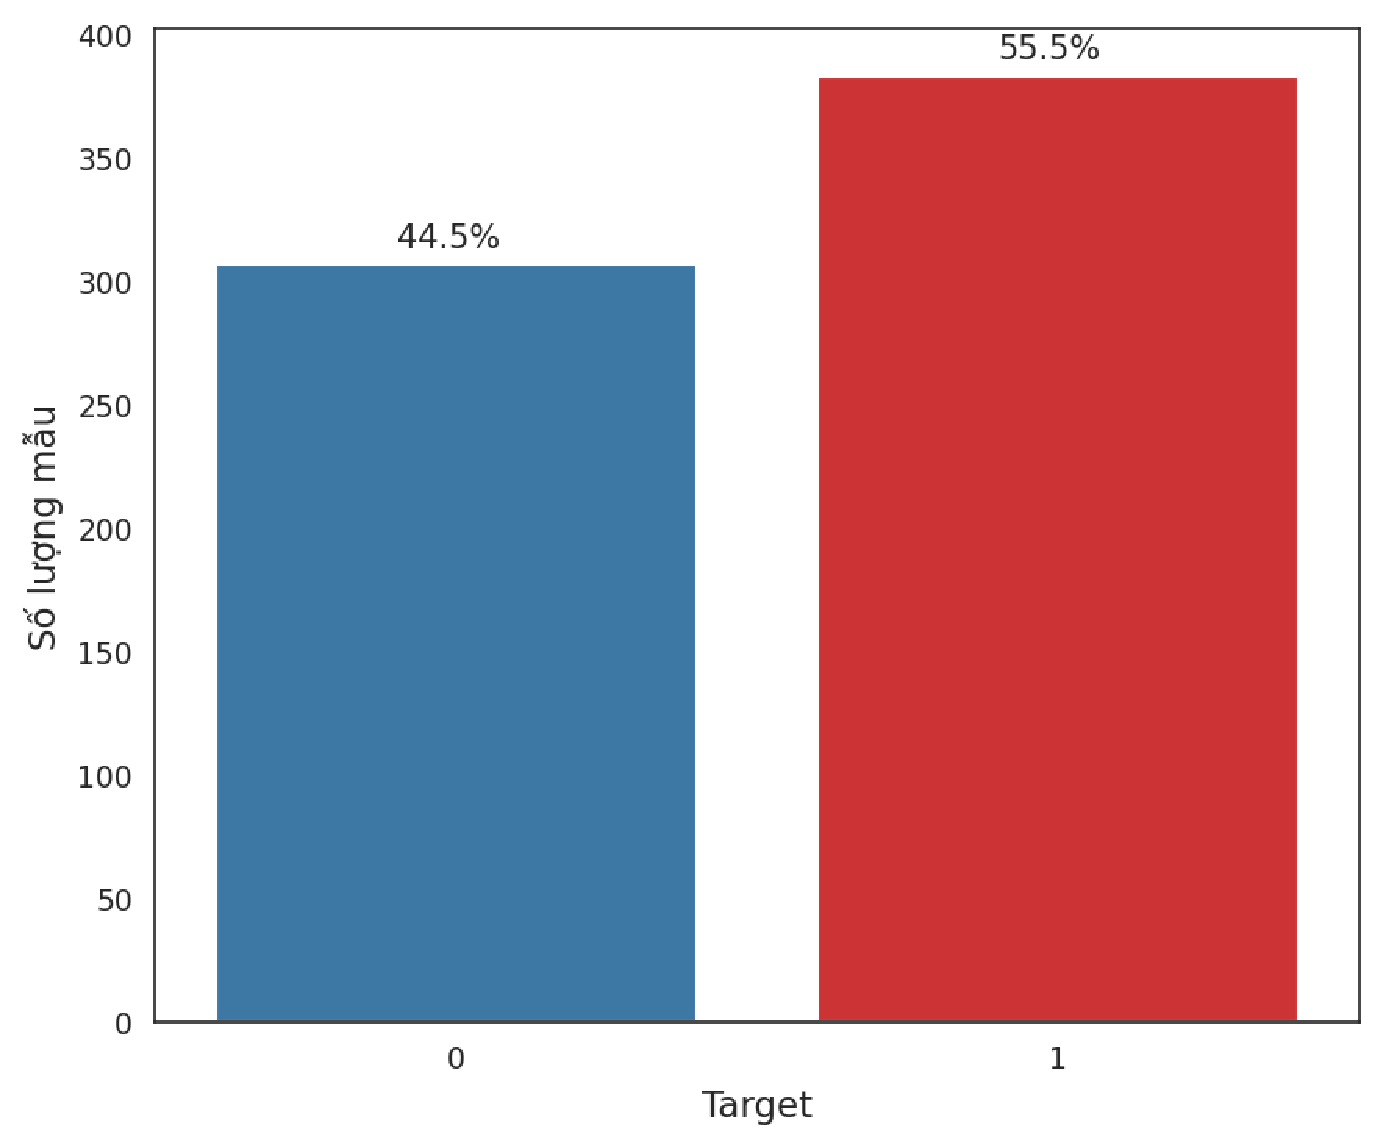
\includegraphics[width=\textwidth]{image/vlz_australian/1_imbalance_au.pdf}
        \caption{Australian Credit}
        \label{fig:imbalance_aus}
    \end{subfigure}
    \hfill
    % Hình 2: German
    \begin{subfigure}[b]{0.43\textwidth}
        \centering
        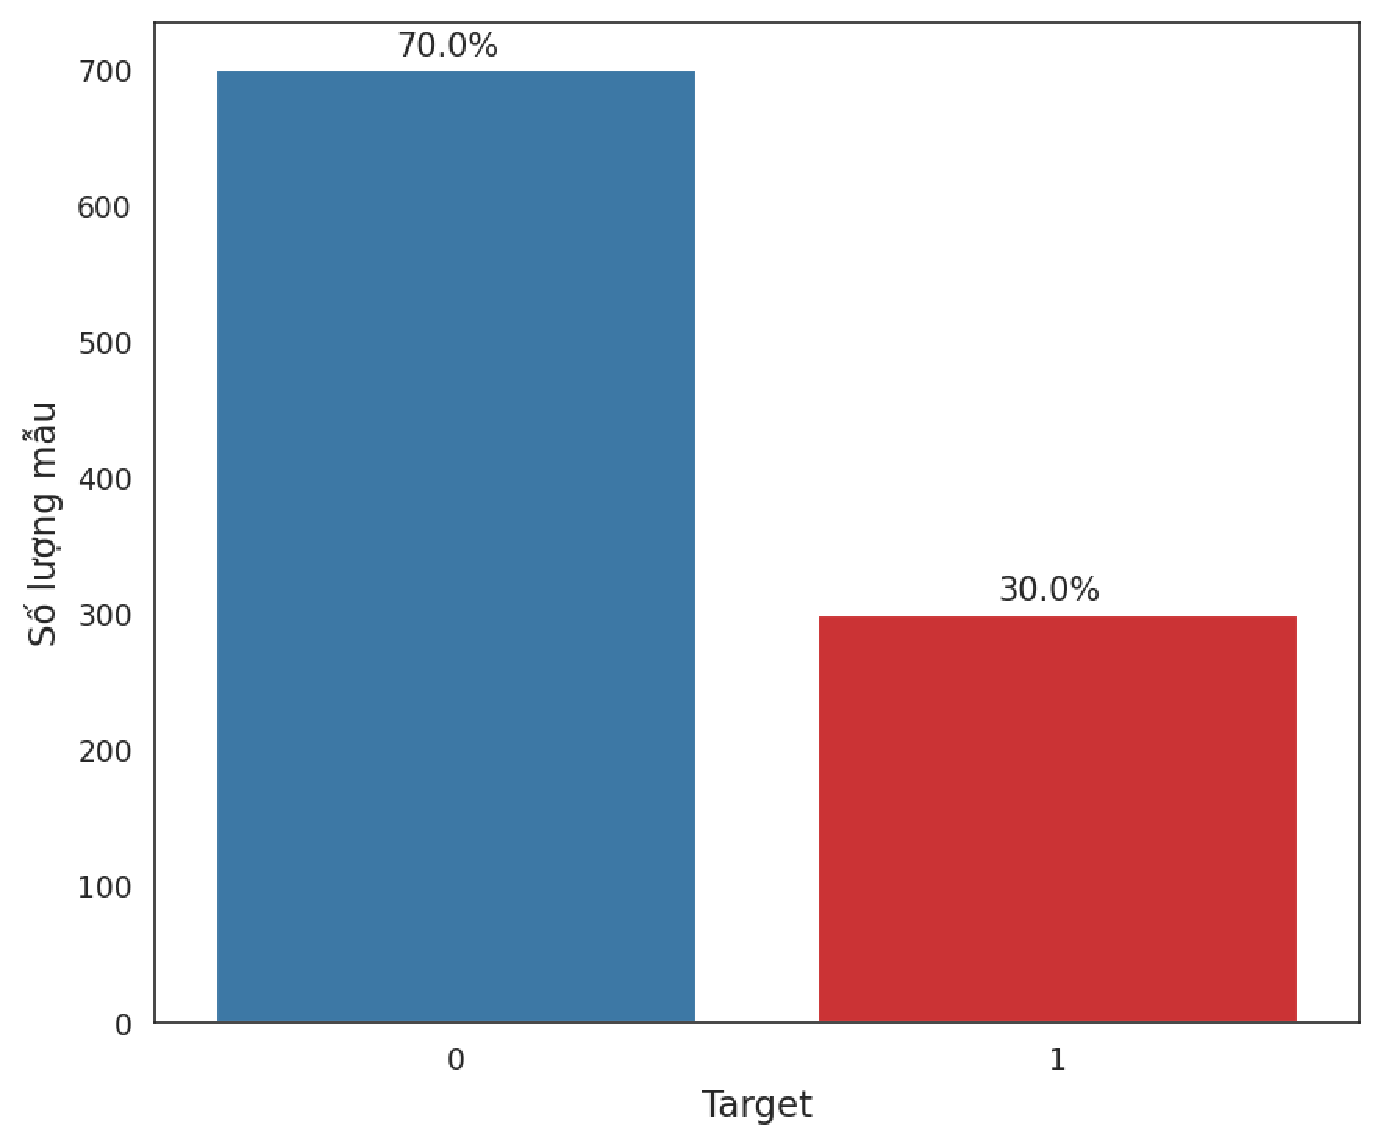
\includegraphics[width=\textwidth]{image/vlz_germany/1_imbalance_ger.pdf}
        \caption{German Credit}
        \label{fig:imbalance_ger}
    \end{subfigure}
    \hfill
    % Hình 3: Lending Club
    \begin{subfigure}[b]{0.43\textwidth}
        \centering
        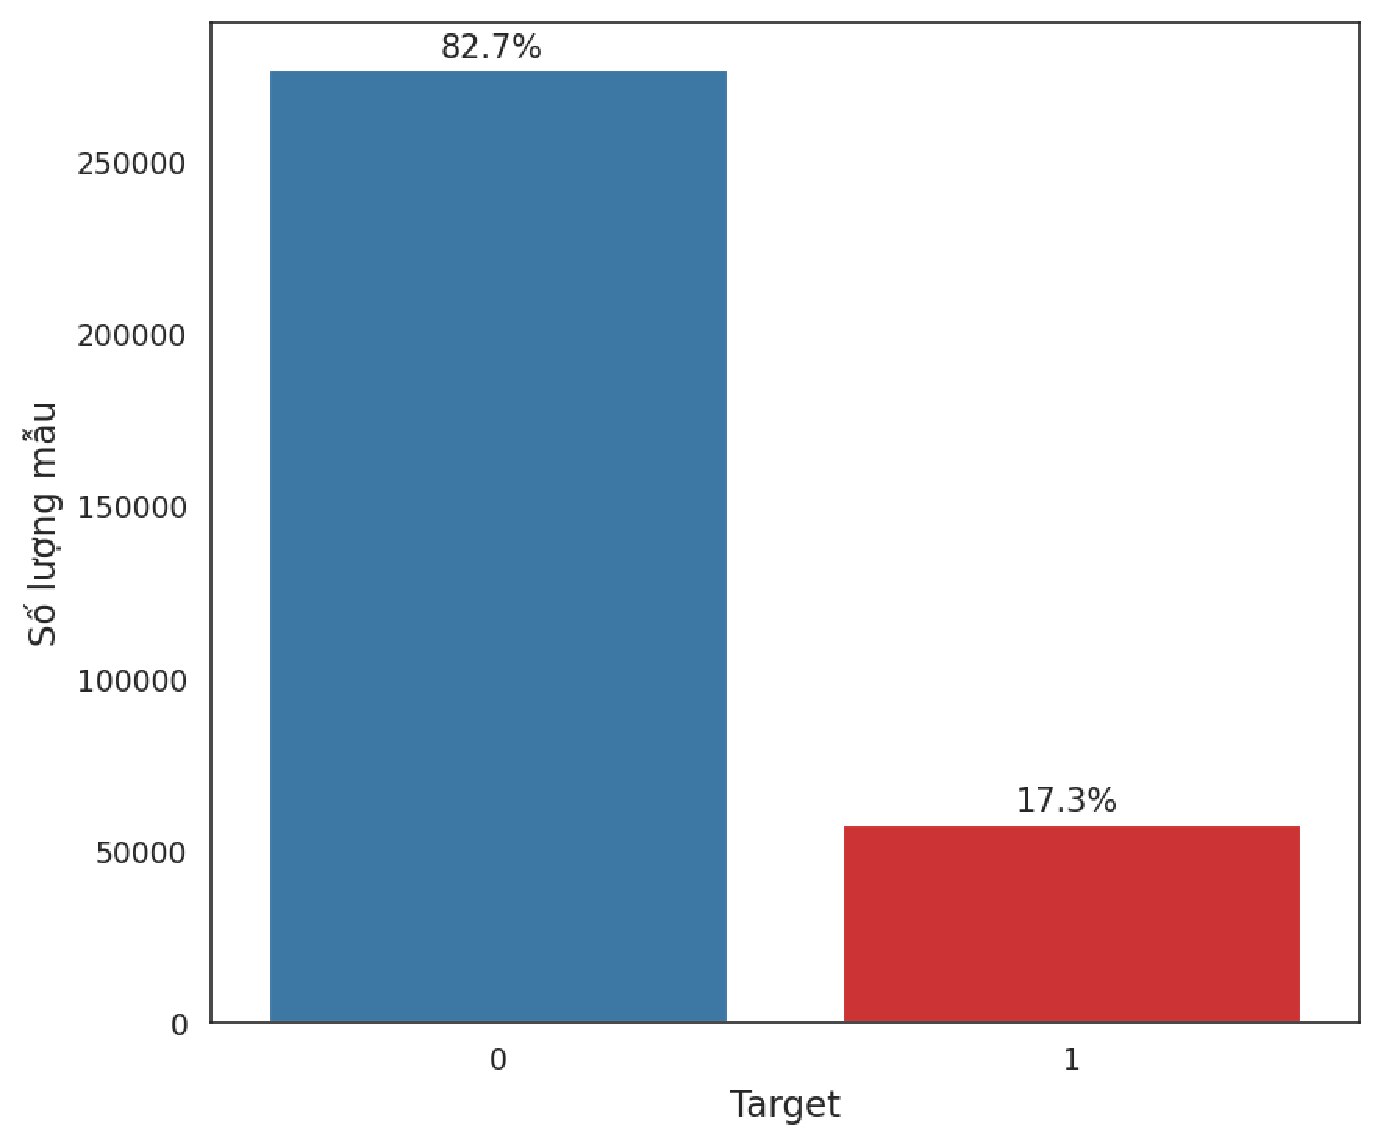
\includegraphics[width=\textwidth]{image/vlz_lending_club/1_imbalance_lend.pdf}
        \caption{Lending Club}
        \label{fig:imbalance_lc}
    \end{subfigure}
    
    \caption{Phân phối nhãn mục tiêu trên ba bộ dữ liệu thực nghiệm}
    \label{fig:class_imbalance}
\end{figure}

\vspace{1em}
Hình \ref{fig:class_imbalance} thể hiện phân phối nhãn mục tiêu của ba bộ dữ liệu. Australian Credit có mức độ cân bằng tốt nhất với tỷ lệ 44.5\% không vỡ nợ và 55.5\% vỡ nợ , gần như đạt cân bằng tự nhiên. German Credit thể hiện sự mất cân bằng vừa phải ở mức 70/30, trong khi tập dữ liệu gốc Lending Club có mức độ mất cân bằng nghiêm trọng nhất với tỷ lệ lên đến 82.7\% không vỡ nợ so với 17.3\% vỡ nợ. Sự chênh lệch này xác nhận sự cần thiết của bước S\_Pro trong đường ống xử lý.

\vspace{1em}
\noindent
\textbf{Phân phối biến liên tục}

Trên bộ dữ liệu Australian (Hình \ref{fig:con_dist_australian}), \texttt{Income} thể hiện phân phối lệch phải cực mạnh. Sau biến đổi $\log(\text{Income} + 1)$, nhóm vỡ nợ tập trung áp đảo ở vùng giá trị rất thấp, trong khi nhóm không vỡ nợ lại phân tán đều hơn và chiếm ưu thế rõ rệt ở các mức thu nhập trung bình và cao. \texttt{Age} tập trung chủ yếu trong độ tuổi 18--35, với nhóm vỡ nợ có xu hướng trẻ hơn, còn nhóm không vỡ nợ mới là nhóm có xu hướng lớn tuổi hơn, thể hiện qua phần đuôi phân phối kéo dài về phía 45--60 tuổi. \texttt{Debt} và \texttt{YearsEmployed} đều lệch phải mạnh, hai nhóm nhãn chồng lấn đáng kể, cho thấy khả năng phân biệt đơn biến hạn chế. Trên bộ dữ liệu German (Hình \ref{fig:con_dist_german}), \texttt{credit\_amount} lệch phải và tập trung dưới 5,000 DM, nhóm vỡ nợ phân tán ở dải giá trị cao hơn. \texttt{month\_duration} thể hiện phân phối đa đỉnh rõ ràng tại các mốc 12, 24 và 36 tháng, phản ánh thực tế các kỳ hạn vay cố định phổ biến, trong đó nhóm vỡ nợ thiên về thời hạn dài hơn. Trên bộ dữ liệu Lending Club (Hình \ref{fig:con_dist_lending}), \texttt{int\_rate} là biến có sức phân biệt rõ nhất trong số các biến liên tục - đường KDE của nhóm vỡ nợ dịch phải đáng kể so với nhóm không vỡ nợ, phản ánh logic tín dụng rằng người vay rủi ro cao bị áp lãi suất cao hơn. \texttt{fico\_range\_low} cho thấy xu hướng ngược lại: điểm tín dụng của nhóm không vỡ nợ cao hơn một cách nhất quán.

% =========================================================================
% KHỐI HÌNH: PHÂN PHỐI CÁC BIẾN LIÊN TỤC THEO TARGET
% =========================================================================
\begin{figure}[htbp]
    \centering
    \begin{subfigure}[b]{\textwidth}
        \centering
        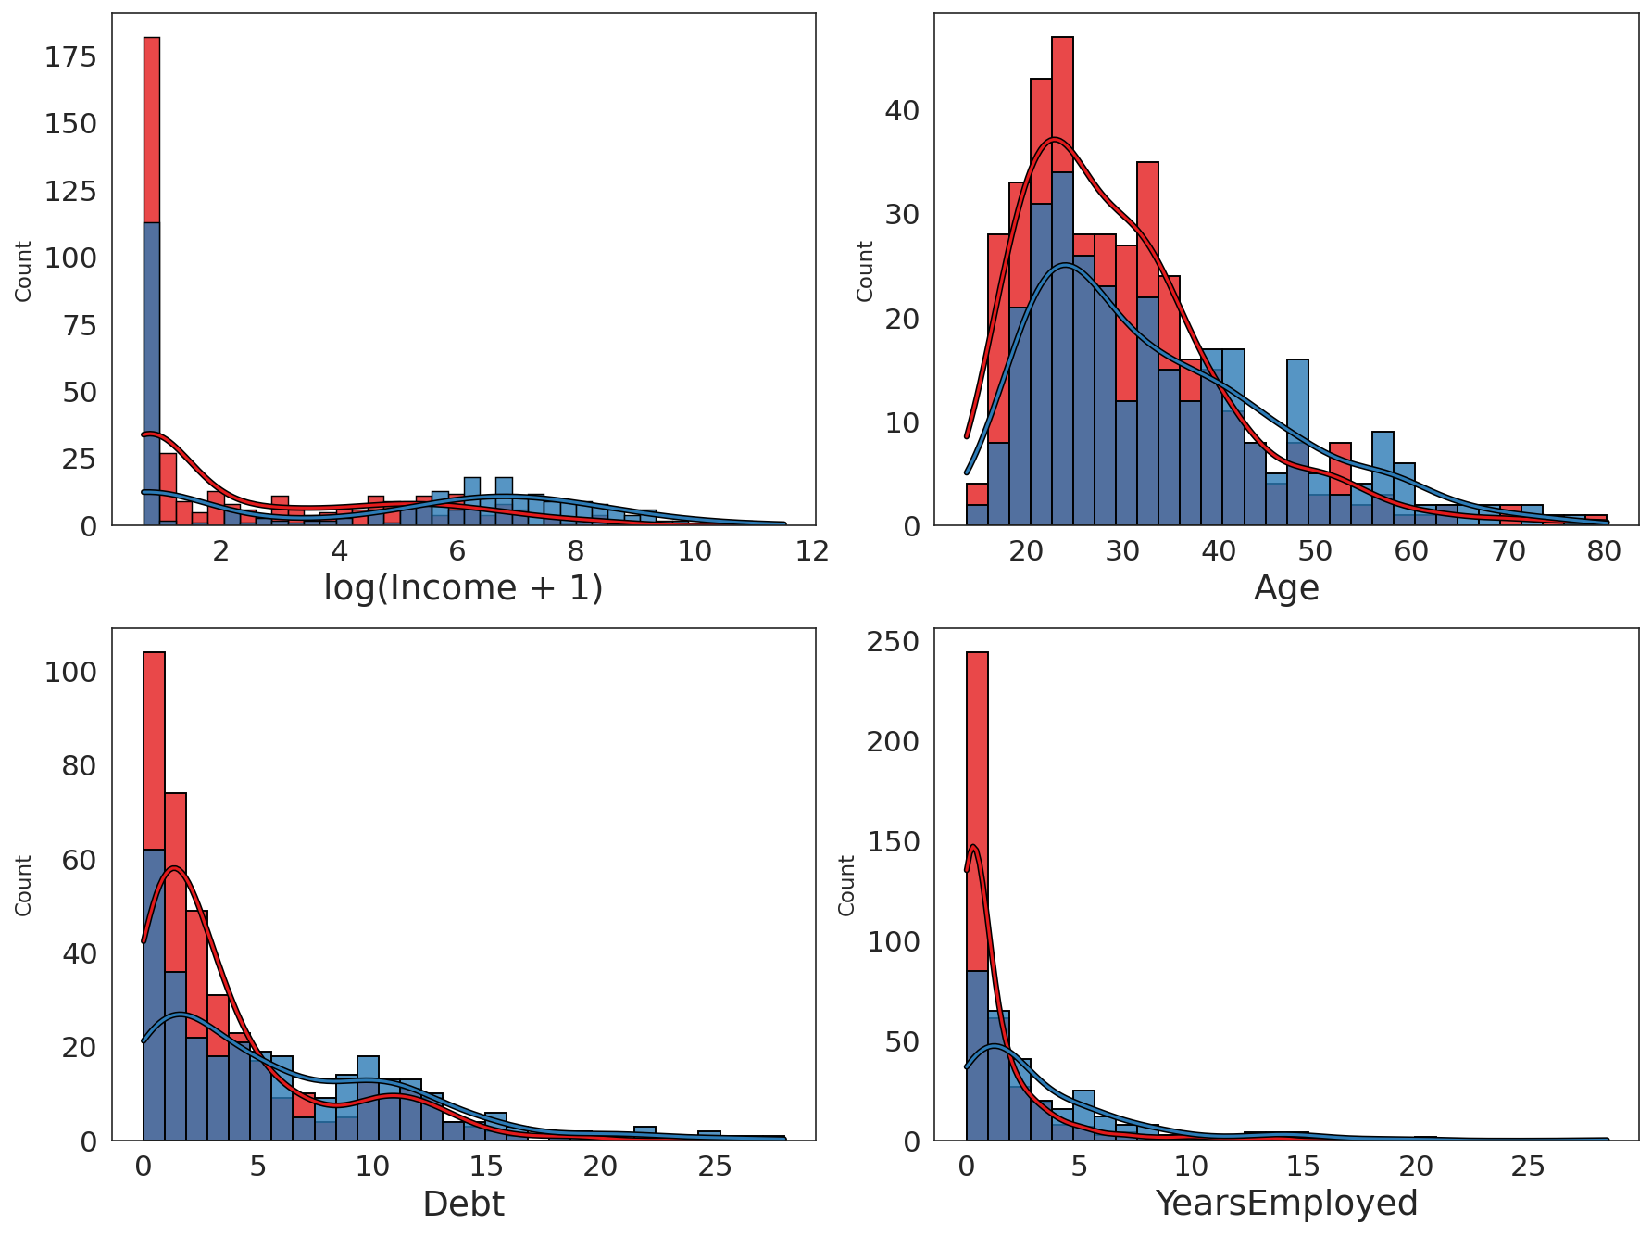
\includegraphics[width=\textwidth]{image/vlz_australian/2_con_dist_au.pdf}
    \end{subfigure}
    
    \caption{Phân phối các biến liên tục theo nhãn \texttt{target} --- Australian Credit. {\newline \small (Trong đó, màu xanh: \texttt{target}~=~0 và màu đỏ: \texttt{target}~=~1)}}
    \label{fig:con_dist_australian}
\end{figure}

\begin{figure}[htbp]
    \centering
    % --- HÀNG 2 ---
    \begin{subfigure}[b]{0.85\textwidth}
        \centering
        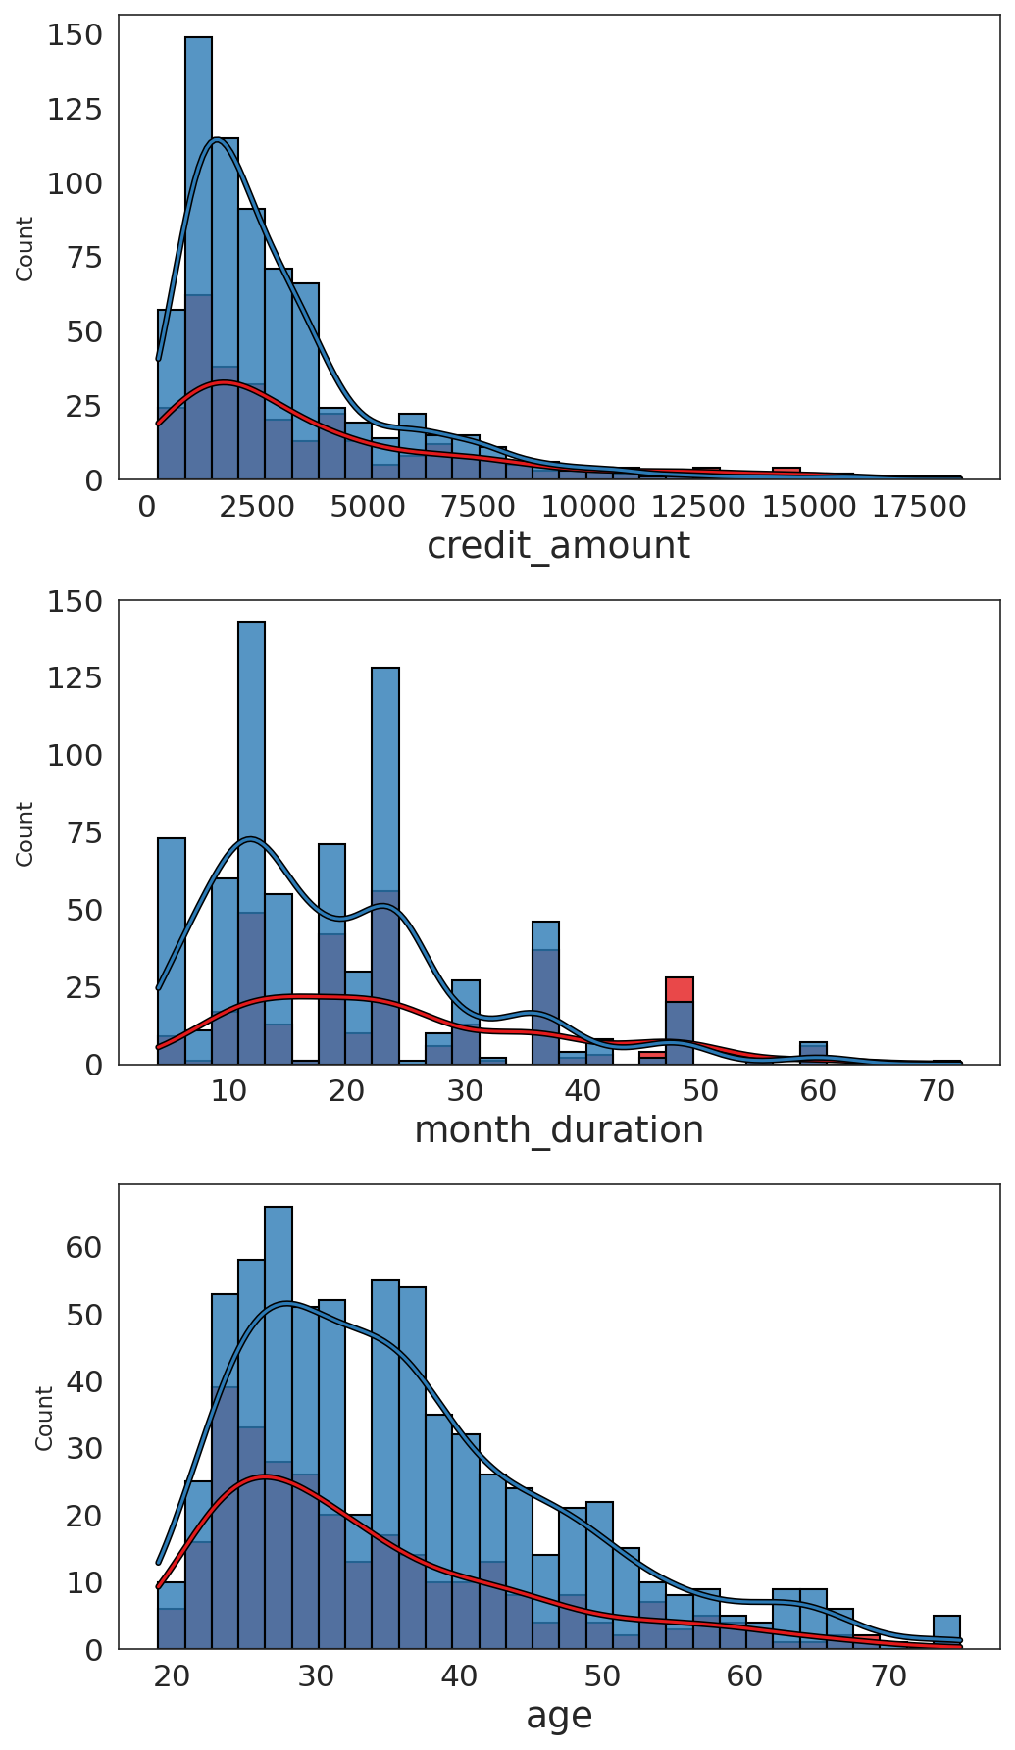
\includegraphics[width=\textwidth]{image/vlz_germany/2_con_dist_ger.pdf}
    \end{subfigure}
    
    \caption{Phân phối các biến liên tục theo nhãn \texttt{target} --- German Credit. {\newline \small (Trong đó, màu xanh: \texttt{target}~=~0 và màu đỏ: \texttt{target}~=~1)}}
    \label{fig:con_dist_german}
\end{figure}

\begin{figure}[htbp]
    \centering
    
    \begin{subfigure}[b]{\textwidth}
        \centering
        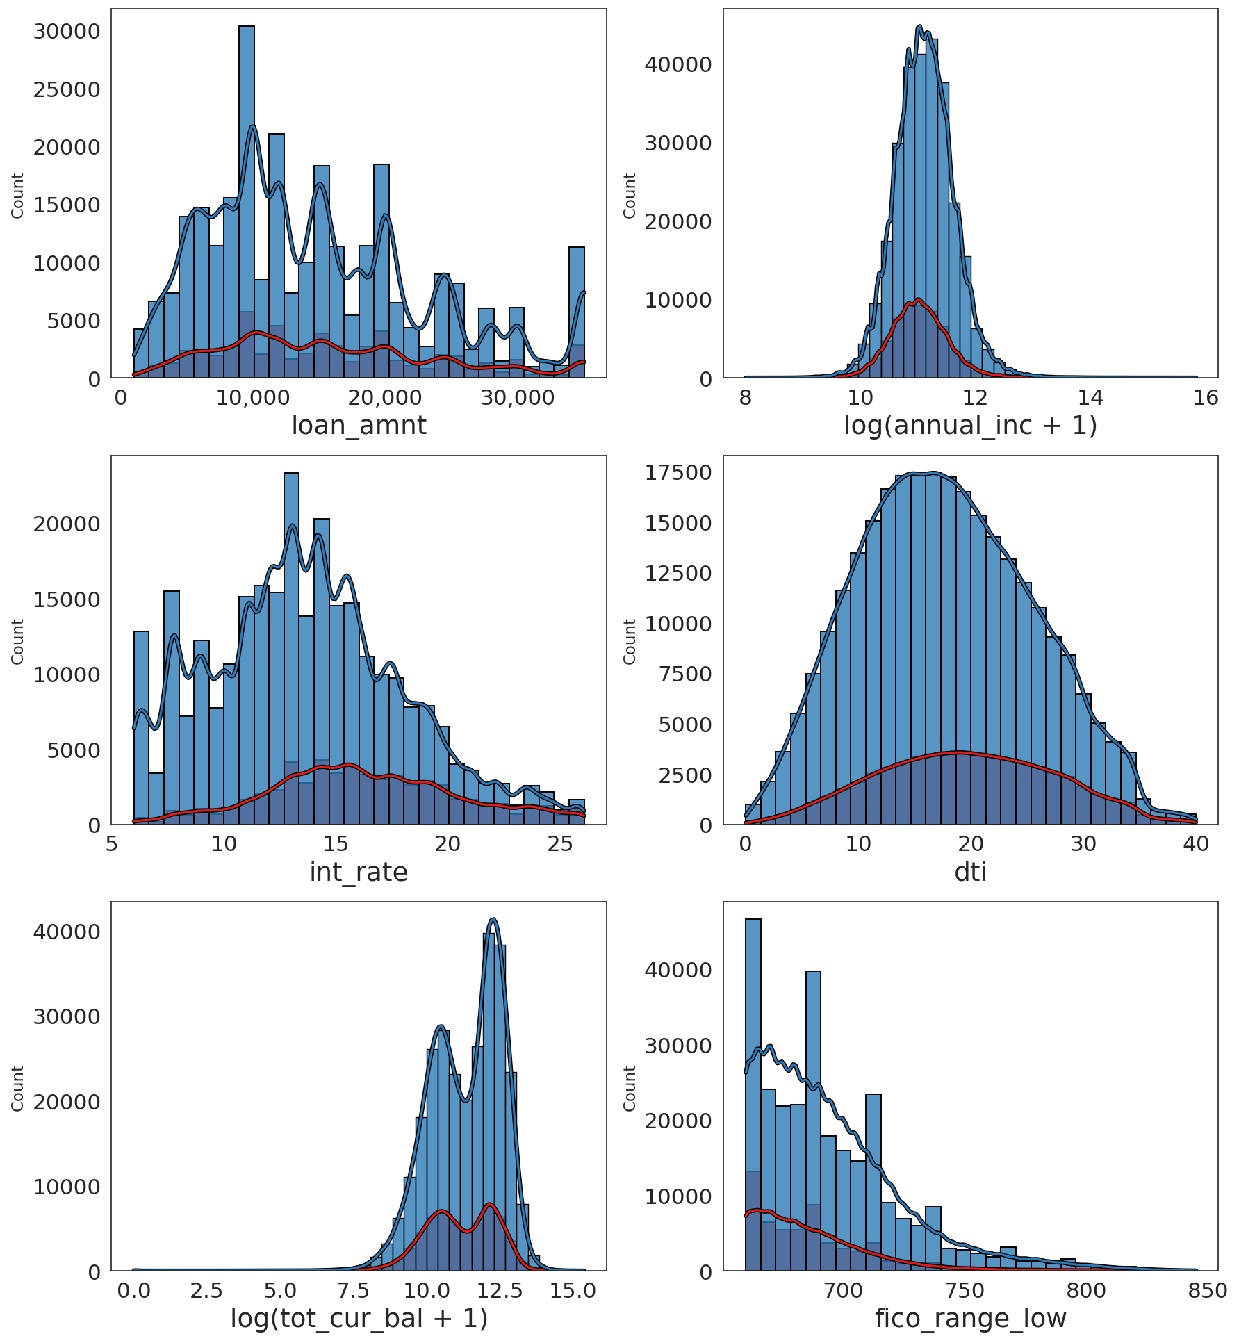
\includegraphics[width=\textwidth]{image/vlz_lending_club/2_con_dist_lend.pdf}
    \end{subfigure}
    
    \caption{Phân phối các biến liên tục theo nhãn \texttt{target} --- Lending Club. {\newline \small (Trong đó, màu xanh: \texttt{target}~=~0 và màu đỏ: \texttt{target}~=~1)}}
    \label{fig:con_dist_lending}
\end{figure}

% =========================================================================
% KHỐI HÌNH: PHÂN PHỐI CÁC BIẾN PHÂN LOẠI THEO TARGET
% =========================================================================
\vspace{0.5em}
\noindent
\textbf{Phân phối biến phân loại} 

Biểu đồ phân phối cho thấy một số biến phân loại có sức phân biệt rủi ro rất rõ ràng. Trên Australian (Hình \ref{fig:cate_dist_australian}), \texttt{CreditHistory} là biến có tính phân biệt cao nhất: nhóm \texttt{CreditHistory} $= 1$ gần như toàn bộ là mẫu không vỡ nợ, trong khi nhóm \texttt{CreditHistory} $= 0$ có tỷ lệ vỡ nợ chiếm ưu thế. \texttt{Employed} cũng thể hiện tính phân biệt tương tự. Trên German (Hình \ref{fig:cate_dist_german}), \texttt{status\_account} là tín hiệu rủi ro mạnh - nhóm không có tài khoản thanh toán (``no checking account'') có tỷ lệ không vỡ nợ áp đảo, trong khi nhóm số dư âm (``$< 0$ DM'') tập trung nhiều mẫu vỡ nợ hơn. \texttt{status\_savings} xác nhận xu hướng tương tự: nhóm tiết kiệm dưới 100 DM chiếm đa số và có tỷ lệ vỡ nợ cao nhất. Trên Lending Club (Hình \ref{fig:cate_dist_lending}), \texttt{grade} là biến phân loại có sức phân biệt mạnh nhất - tỷ lệ vỡ nợ tăng đơn điệu từ hạng A đến G, cho thấy hệ thống xếp hạng nội bộ của Lending Club có tương quan trực tiếp với rủi ro thực tế. Khoản vay 60 tháng cũng có tỷ lệ vỡ nợ cao hơn rõ so với 36 tháng.

\vspace{1.5em}
\begin{figure}[htbp]
    \centering

    \begin{subfigure}[b]{\textwidth}
        \centering
        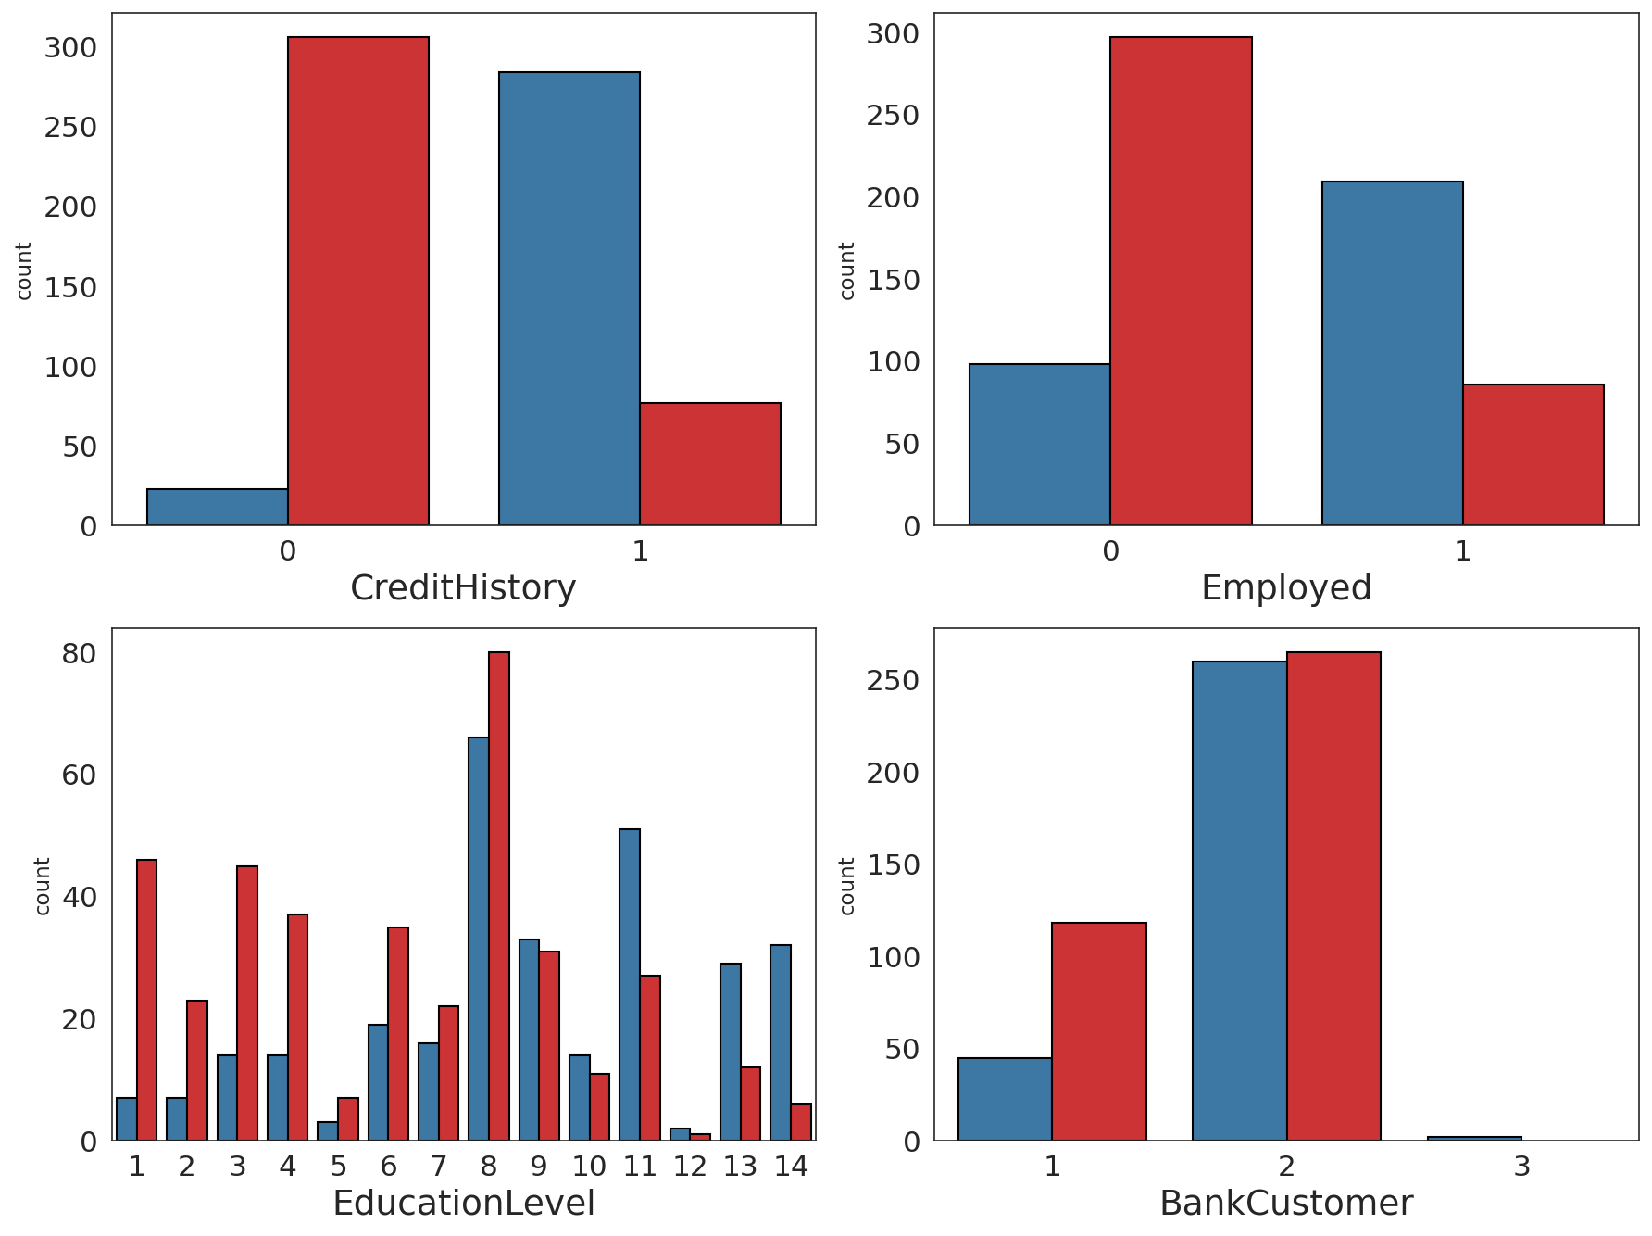
\includegraphics[width=\textwidth]{image/vlz_australian/3_cate_dist_au.pdf}
    \end{subfigure}
    
    \caption{Phân phối các biến phân loại theo nhãn \texttt{target} --- Australian Credit. {\newline \small (Trong đó, màu xanh: \texttt{target}~=~0 và màu đỏ: \texttt{target}~=~1)}}
    \label{fig:cate_dist_australian}
\end{figure}

\begin{figure}[htbp]
    \centering
    
    \begin{subfigure}[b]{\textwidth}
        \centering
        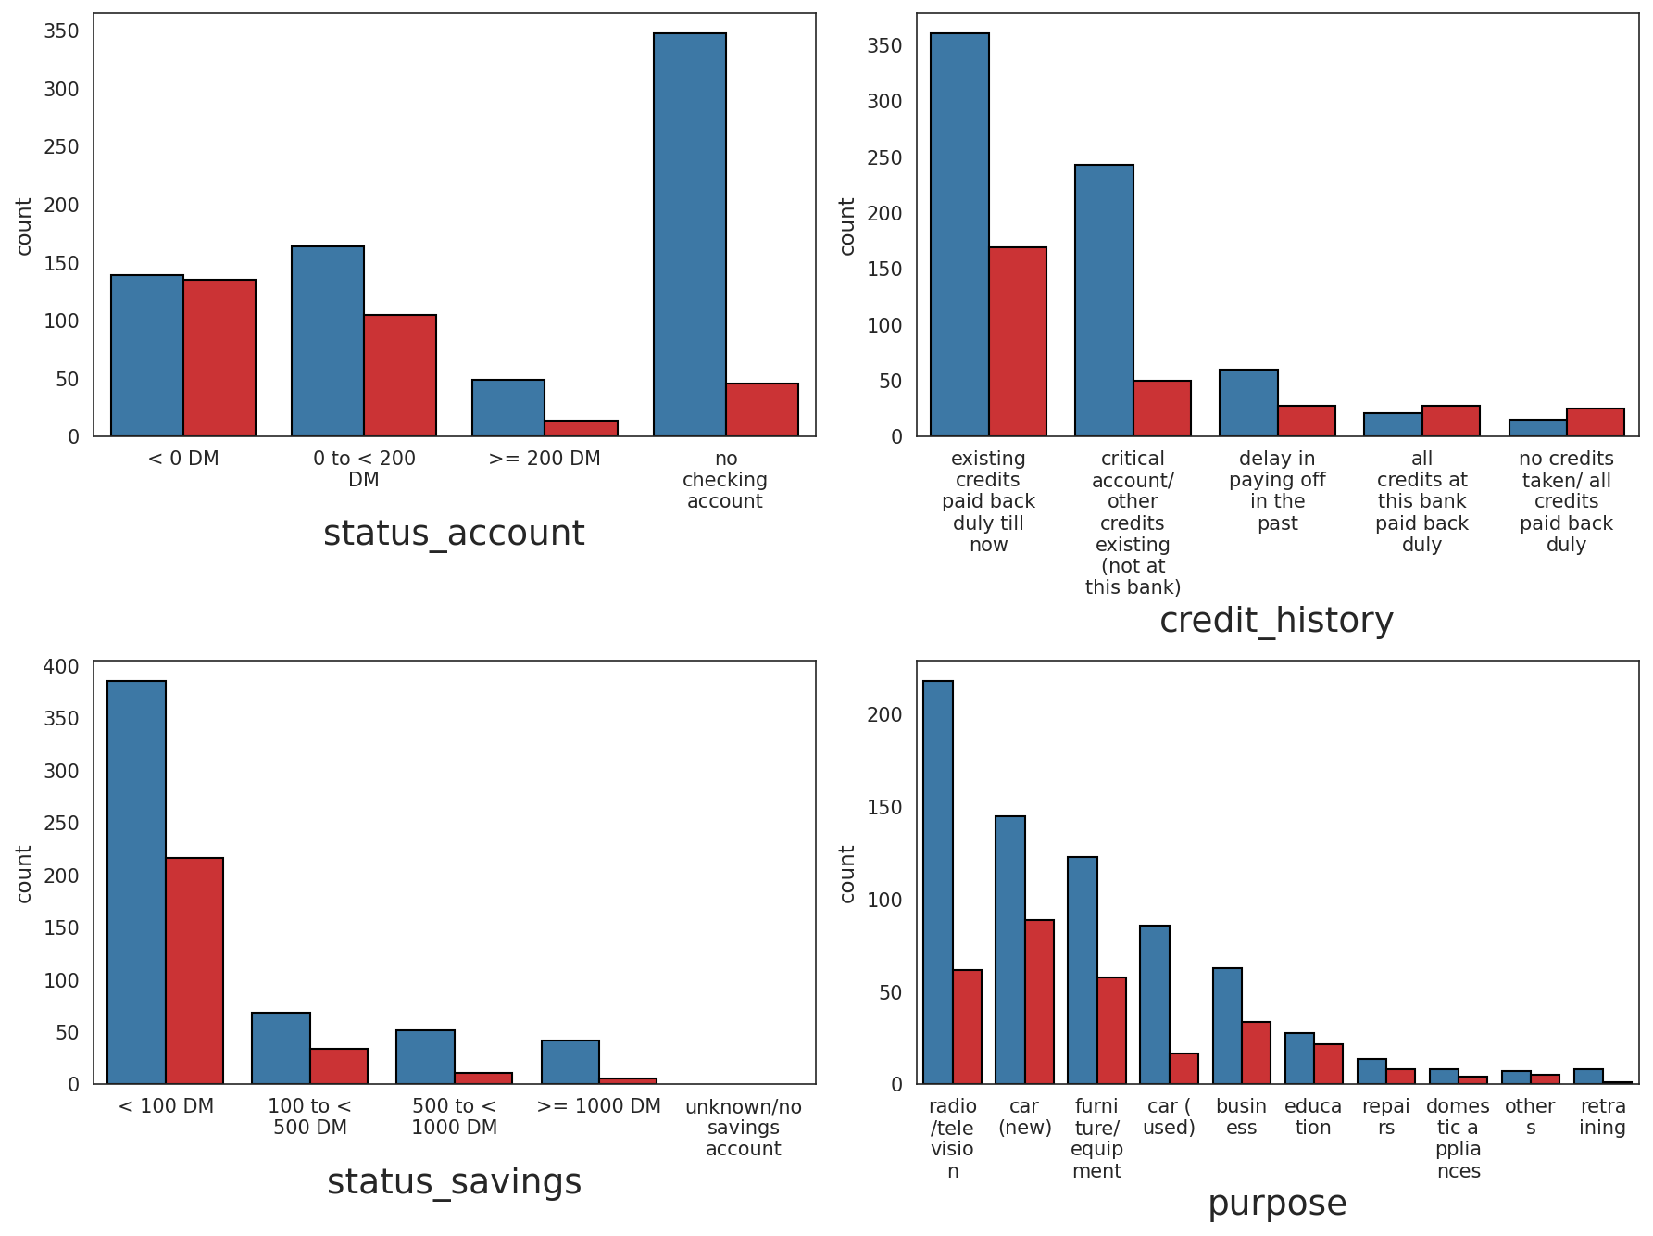
\includegraphics[width=\textwidth,
        height=0.45\textheight]{image/vlz_germany/3_cate_dist_ger.pdf}
    \end{subfigure}
    
    \caption{Phân phối các biến phân loại theo nhãn \texttt{target} --- German Credit. {\newline \small (Trong đó, màu xanh: \texttt{target}~=~0 và màu đỏ: \texttt{target}~=~1)}}
    \label{fig:cate_dist_german}
\end{figure}

\begin{figure}[htbp]
    \centering
    \begin{subfigure}[b]{\textwidth}
        \centering
        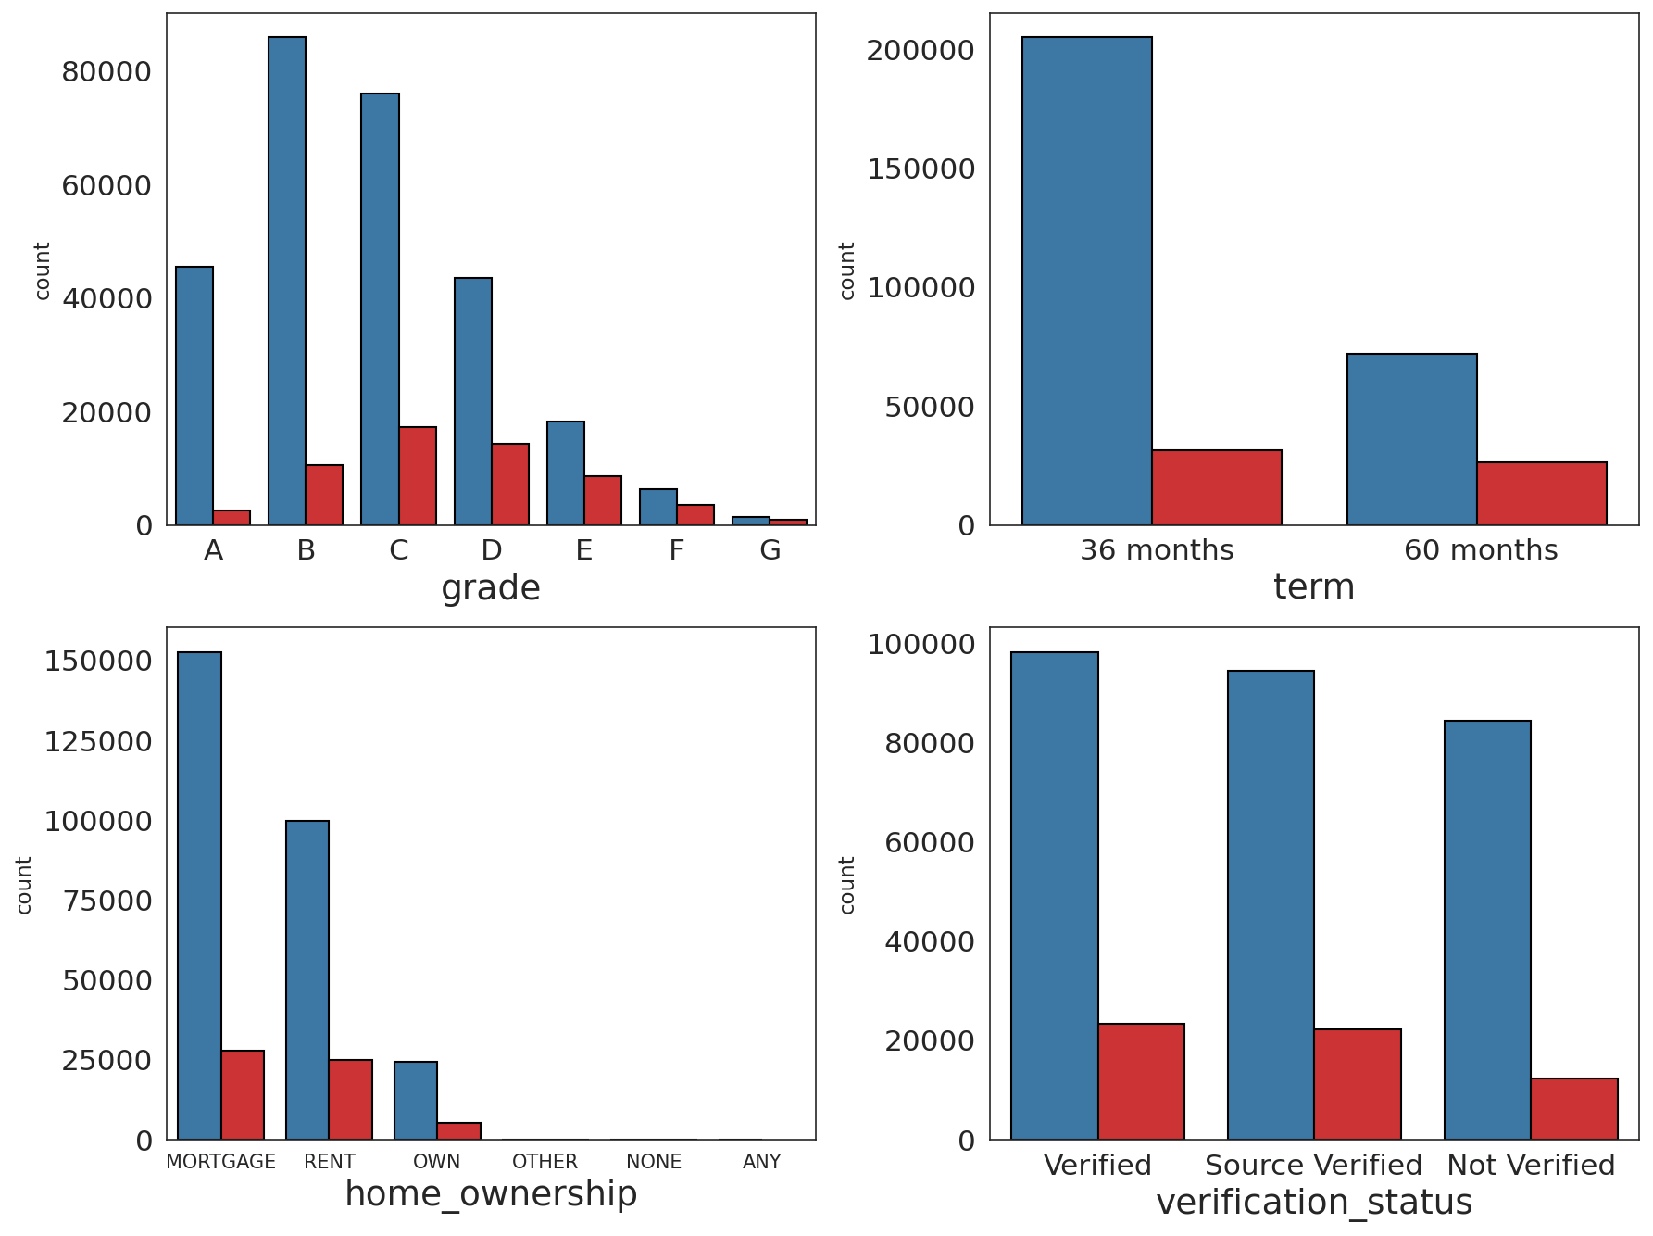
\includegraphics[width=\textwidth,
        height=0.4\textheight,]{image/vlz_lending_club/3_cate_dist_lend.pdf}
    \end{subfigure}
    
    \caption{Phân phối các biến phân loại theo nhãn \texttt{target} --- Lending Club. {\newline \small (Trong đó, màu xanh: \texttt{target}~=~0 và màu đỏ: \texttt{target}~=~1)}}
    \label{fig:cate_dist_lending}
\end{figure}

% =========================================================================
% KHỐI HÌNH: TƯƠNG QUAN
% =========================================================================
\FloatBarrier
\vspace{0.5em}
\noindent
\textbf{Ma trận tương quan} 

Trên Australian (Hình \ref{fig:corr_aus}), hầu hết các cặp biến có tương quan rất thấp, ngoại trừ cặp \texttt{YearsEmployed}-\texttt{Employed} có tương quan dương vừa phải, phản ánh mối liên hệ tự nhiên giữa tình trạng việc làm và thâm niên. Trên German (Hình \ref{fig:corr_ger}), cặp \texttt{month\_duration} và \texttt{credit\_amount} có tương quan dương đáng chú ý - khoản vay lớn hơn thường đi kèm với thời hạn hoàn trả dài hơn, một quan hệ hợp lý về mặt nghiệp vụ tín dụng. Trên Lending Club (Hình \ref{fig:corr_lend}), không gian biến rộng hơn nhiều với 36 biến số, xuất hiện một số cụm tương quan nội bộ giữa các biến cùng nhóm như nhóm biến đếm tài khoản (\texttt{num\_bc\_tl}, \texttt{num\_il\_tl}, \texttt{num\_actv\_rev\_tl}) và nhóm biến thời gian tháng. Đặc biệt, cặp \texttt{fico\_range\_low} và \texttt{int\_rate} có tương quan âm rõ ràng, phản ánh đúng cơ chế định giá rủi ro: điểm tín dụng cao tương ứng với lãi suất thấp hơn. Sự hiện diện của các cụm tương quan này là động lực cho bước L\_Pro sau này.

\vspace{1em}
\begin{figure}[htbp]
    \centering
    \begin{subfigure}[b]{\textwidth}
        \centering
        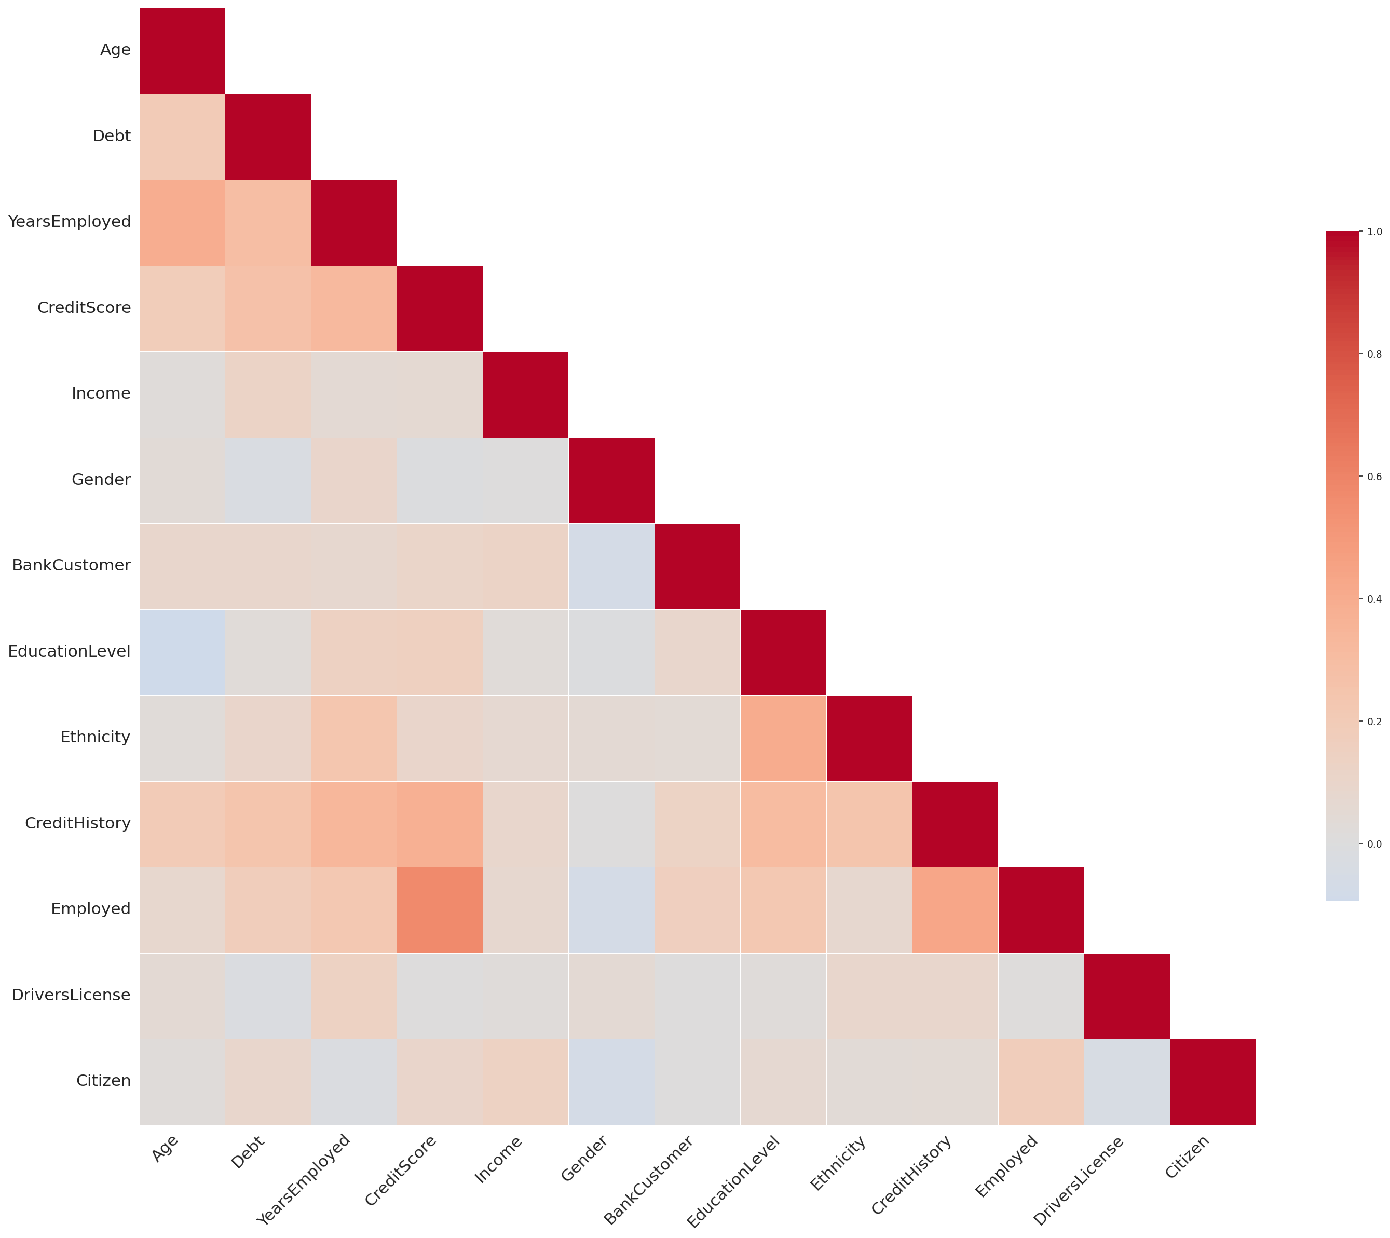
\includegraphics[width=\textwidth]{image/vlz_australian/4_cor_au.pdf}
    \end{subfigure}
    \caption{Ma trận tương quan giữa các biến số liên tục trên Australian Credit}
    \label{fig:corr_aus}
\end{figure}

\begin{figure}[htbp]
    \centering
    \begin{subfigure}[b]{\textwidth}
        \centering
        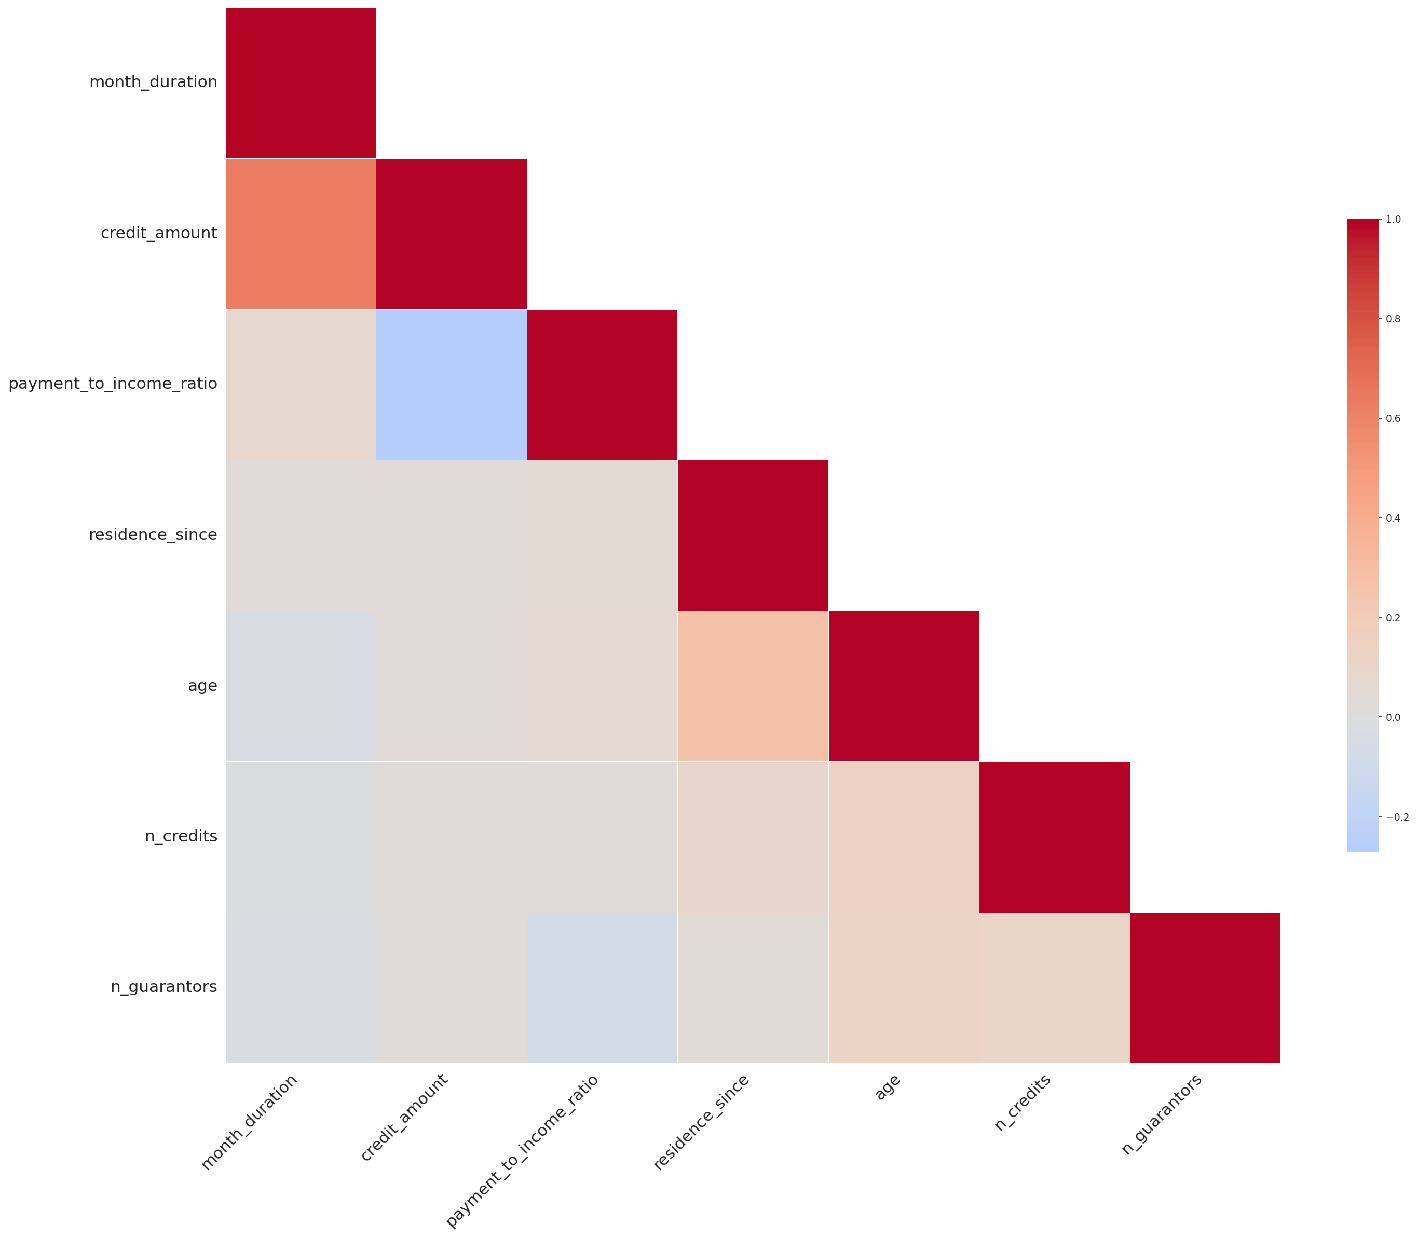
\includegraphics[width=\textwidth]{image/vlz_germany/4_cor_ger.pdf}
    \end{subfigure}
    
    \caption{Ma trận tương quan giữa các biến số liên tục trên German Credit}
    \label{fig:corr_ger}
\end{figure}

\newpage
\begin{figure}[htbp]
    \centering
    \begin{subfigure}[b]{\textwidth}
        \centering
        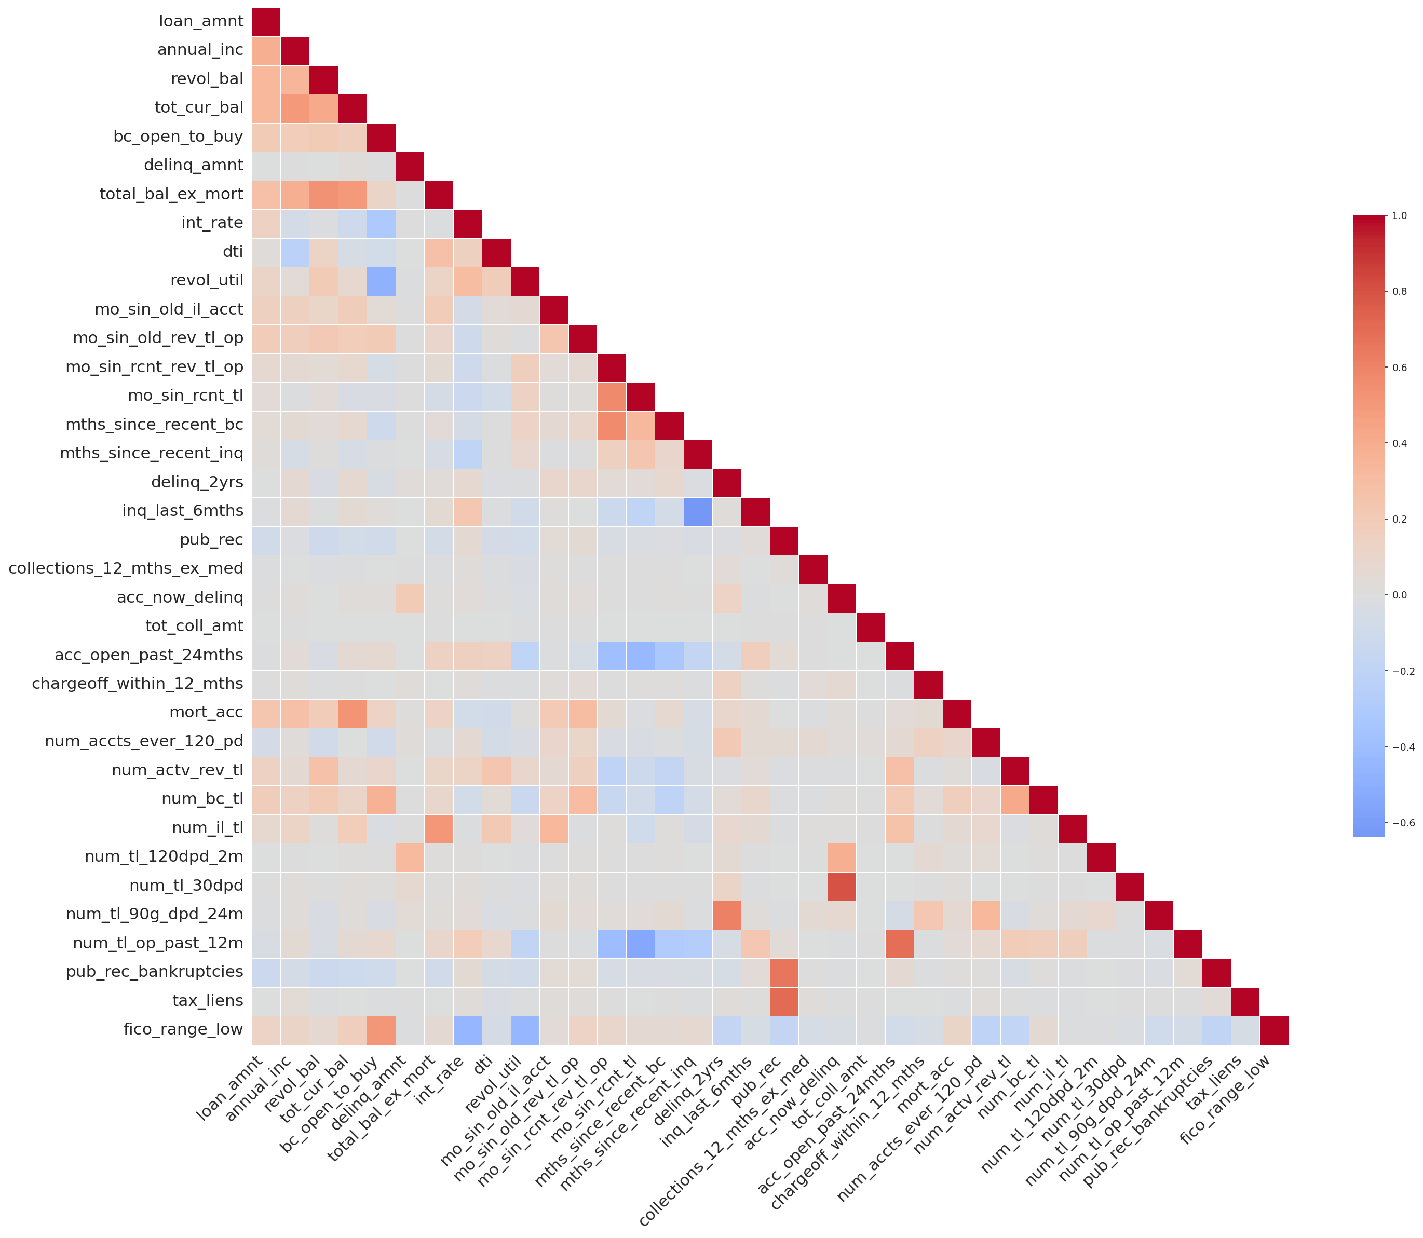
\includegraphics[width=\textwidth]{image/vlz_lending_club/4_cor_lend.pdf}
    \end{subfigure}
    
    \caption{Ma trận tương quan giữa các biến số liên tục trên Lending Club}
    \label{fig:corr_lend}
\end{figure}

\subsection{Xử lý dữ liệu}
\subsubsection{Mã hóa đặc trưng phân loại}
\noindent
Trước khi đưa dữ liệu vào pipelines xử lý dữ liệu, các biến phân loại cần được chuyển hóa thành dạng số để các thuật toán có thể xử lý. Tuy nhiên, không phải mọi biến phân loại đều có thể được mã hóa theo cùng một cách. Nghiên cứu này phân biệt rõ hai nhóm đặc trưng theo bản chất thống kê: biến thứ tự (ordinal) có quan hệ phân cấp nội tại giữa các giá trị, và biến danh nghĩa (nominal) không có thứ bậc tự nhiên giữa các nhóm. Việc áp dụng nhầm phương pháp mã hóa cho từng loại có thể đưa vào mô hình các quan hệ thứ tự giả tạo, dẫn đến sai lệch trong học cấu trúc mạng Bayes.

Đối với bộ dữ liệu Australian, toàn bộ biến phân loại trong tập dữ liệu gốc đã được mã hóa sẵn dưới dạng số nguyên, do đó không cần thực hiện bước mã hóa bổ sung.

Đối với bộ dữ liệu German, năm biến thứ tự được mã hóa thủ công theo ánh xạ phân cấp có ý nghĩa nghiệp vụ. Cụ thể, \texttt{status\_account} được ánh xạ theo mức độ số dư tài khoản từ âm đến dương (0: dưới 0 DM $\rightarrow$ 3: không có tài khoản thanh toán); \texttt{credit\_history} được sắp xếp theo mức độ tin cậy tín dụng tăng dần từ tài khoản có vấn đề đến lịch sử thanh toán hoàn hảo; \texttt{status\_savings} phản ánh quy mô tiết kiệm tăng dần; \texttt{years\_employment} biểu diễn thâm niên làm việc từ thất nghiệp đến trên 7 năm; \texttt{job} thể hiện bậc nghề nghiệp từ lao động phổ thông đến quản lý cấp cao. Tám biến danh nghĩa còn lại gồm \texttt{purpose}, \texttt{status\_and\_sex}, \texttt{secondary\_obligor}, \texttt{collateral}, \texttt{other\_installment\_plans}, \texttt{housing}, \texttt{telephone} và \texttt{is\_foreign\_worker} không có quan hệ thứ bậc tự nhiên giữa các giá trị, do đó được mã hóa tự động bằng \texttt{OrdinalEncoder} với vai trò định danh số nguyên thuần túy. Cách tiếp cận này phù hợp với yêu cầu của mạng Bayes vì mô hình học cấu trúc xác suất từ tần suất quan sát thực tế, không giả định quan hệ tuyến tính giữa các giá trị mã hóa.

Đối với bộ dữ liệu Lending Club, bốn biến thứ tự được ánh xạ thủ công theo logic nghiệp vụ rõ ràng. \texttt{grade} được ánh xạ từ A (0) đến G (6) theo chiều rủi ro tăng dần, phản ánh đúng hệ thống xếp hạng tín dụng nội bộ của Lending Club. \texttt{emp\_length} biểu diễn thâm niên làm việc từ không xác định (0) đến trên 10 năm (11). \texttt{verification\_status} phản ánh mức độ xác minh thu nhập tăng dần từ chưa xác minh đến đã xác minh đầy đủ. \texttt{term} mã hóa kỳ hạn vay với 36 tháng là 0 và 60 tháng là 1. Sáu biến danh nghĩa gồm \texttt{home\_ownership}, \texttt{purpose}, \texttt{addr\_state}, \texttt{initial\_list\_status}, \texttt{debt\_settlement\_flag} và \texttt{hardship\_flag} được mã hóa tự động bằng \texttt{OrdinalEncoder}. Ngoài ra, biến thời gian \texttt{earliest\_cr\_line} lưu dưới dạng chuỗi tháng-năm được chuyển hóa thành biến số liên tục \texttt{mths\_since\_earliest\_cr} - số tháng tính từ thời điểm mở dòng tín dụng đầu tiên đến mốc tham chiếu tháng 1/2015, qua đó bảo toàn thông tin thâm niên tín dụng dưới dạng có thể so sánh định lượng.

\subsubsection{Chia tập huấn luyện và kiểm tra}
\noindent
Để đảm bảo tính khách quan trong đánh giá mô hình, toàn bộ dữ liệu được chia thành các tập con riêng biệt trước khi áp dụng bất kỳ bước tiền xử lý nào liên quan đến máy học. Cả ba bộ dữ liệu đều sử dụng tỷ lệ chia 60/40, trong đó 60\% được dùng làm tập huấn luyện và 40\% còn lại được giữ lại làm tập kiểm tra. Việc chia tập được thực hiện trước các bước SMOTE, Lasso và K-means nhằm tránh hiện tượng rò rỉ dữ liệu (data leakage) — tức là thông tin từ tập kiểm tra vô tình ảnh hưởng đến quá trình huấn luyện mô hình, dẫn đến đánh giá hiệu suất lạc quan giả tạo.

\begin{table}[htbp]
    \centering
    \caption{Phân phối biến mục tiêu sau khi chia tập dữ liệu}
    \label{tab:train_test_split}
    \renewcommand{\arraystretch}{1.3} % Tăng khoảng cách các dòng để bảng thoáng và đẹp hơn
    \begin{tabular}{|l|c|c|c|c|}
        \hline
        \textbf{Bộ dữ liệu} & \textbf{Tập} & \textbf{Không vỡ nợ} & \textbf{Vỡ nợ} & \textbf{Tổng} \\ 
        \hline
        \multirow{3}{*}{Australian} 
        & Train & 197 & 217 & 414 \\ \cline{2-5}
        & Val & 58 & 80 & 138 \\ \cline{2-5}
        & Test  & 52 & 86 & 138 \\ 
        \hline
        \multirow{3}{*}{German} 
        & Train & 418 & 182 & 600 \\ \cline{2-5}
        & Val & 145 & 55 & 200 \\ \cline{2-5}
        & Test  & 137 & 63 & 200 \\ 
        \hline
        \multirow{3}{*}{Lending Club} 
        & Train & 12,579 & 5,421 & 18,000 \\ \cline{2-5}
        & Val & 4,190 & 1,810 & 6,000 \\ \cline{2-5}
        & Test  & 4,231  & 1,769 & 6,000 \\ 
        \hline
    \end{tabular}
\end{table}

Sau khi toàn bộ đường ống tiền xử lý hoàn tất, tập kiểm tra ban đầu (40\%) sẽ được chia tiếp thành hai phần bằng nhau. Phần thứ nhất đóng vai trò tập validation dùng để tinh chỉnh ngưỡng phân loại, trong khi phần thứ hai được giữ nguyên làm tập test thực sự để báo cáo kết quả cuối cùng. Như vậy, tỷ lệ phân chia tổng thể là 60\% huấn luyện, 20\% validation và 20\% kiểm tra.

\subsubsection{Cân bằng dữ liệu (S\_Pro)}
\noindent
Như đã phân tích tại \ref{fig:class_imbalance}, ba bộ dữ liệu thực nghiệm đều biểu hiện mức độ mất cân bằng lớp ở các mức độ khác nhau. Sự chênh lệch này, nếu không được xử lý, sẽ khiến quá trình học cấu trúc mạng Bayes bị lệch về phía lớp đa số, dẫn đến bảng xác suất có điều kiện ước lượng thiên vị và suy giảm khả năng nhận diện rủi ro thực sự. Do đó, bước S\_Pro được áp dụng trên tập huấn luyện ngay sau khi chia tập, trước mọi thao tác tiền xử lý tiếp theo, nhằm đảm bảo không có thông tin từ tập kiểm tra rò rỉ vào quá trình tổng hợp mẫu.

Một điểm kỹ thuật quan trọng là cả ba bộ dữ liệu đều chứa hỗn hợp giữa biến liên tục và biến phân loại. Thuật toán SMOTE tiêu chuẩn \citep{chawla2002smote} vốn được thiết kế cho không gian đặc trưng thuần liên tục, với cơ chế nội suy tuyến tính theo công thức \ref{eq:3.1} khi áp dụng trực tiếp lên biến phân loại sẽ tạo ra các giá trị trung gian vô nghĩa về mặt ngữ nghĩa, chẳng hạn như một trạng thái tài khoản mang giá trị thập phân 2.4 hay một mã mục đích vay bằng 1.73. Để khắc phục hạn chế này, nghiên cứu sử dụng biến thể SMOTE-NC (Synthetic Minority Over-sampling Technique for Nominal and Continuous features). Với mỗi mẫu tổng hợp mới, các biến liên tục vẫn được nội suy theo Công thức \ref{eq:3.1}, trong khi giá trị của từng biến phân loại được quyết định bằng cơ chế bỏ phiếu đa số (majority voting) trên tập $k$ láng giềng gần nhất, tức là chọn giá trị phân loại xuất hiện nhiều nhất trong vùng lân cận của mẫu gốc, qua đó đảm bảo tính hợp lệ về mặt ngữ nghĩa của các quan sát được sinh ra. Mã giả của thuật toán được trình bày như sau:

\vspace{0.5em}
\begin{algorithm}[H]
\caption{Mã giả của thuật toán SMOTE-NC}
\label{alg:smote_nc}

\vspace{0.5em}
\textbf{Input:} Tập mẫu thiểu số $X_{min}$, tập chỉ số biến phân loại $\mathcal{C}$, số láng giềng $k$, tỷ lệ tổng hợp $N$.

\vspace{0.5cm}

\textbf{Output:} Tập mẫu tổng hợp $X_{syn}$.

\begin{tcolorbox}
\begin{algorithmic}[1]
    \State $X_{syn} \gets \emptyset$
    \For{mỗi $x_i \in X_{min}$}
        \State Tính khoảng cách từ $x_i$ đến các mẫu khác trong $X_{min}$, trong đó biến liên tục dùng khoảng cách Euclidean và biến phân loại dùng giá trị $0$ (cùng nhãn) hoặc $\sigma_c$ (khác nhãn, với $\sigma_c$ là độ lệch chuẩn của toàn bộ biến liên tục)
        \State Xác định $k$ láng giềng gần nhất $\mathcal{N}(x_i)$
        \For{$n = 1$ đến $N$}
            \State Chọn ngẫu nhiên $x_{nn}$ từ $\mathcal{N}(x_i)$
            \State Lấy mẫu $\lambda \sim \mathcal{U}(0, 1)$
            \For{mỗi đặc trưng $j$}
                \If{$j \notin \mathcal{C}$} \Comment{Biến liên tục}
                    \State $x_{new}^{(j)} \gets x_i^{(j)} + \lambda \cdot (x_{nn}^{(j)} - x_i^{(j)})$
                \Else \Comment{Biến phân loại}
                    \State $x_{new}^{(j)} \gets \text{mode}\bigl(\{x^{(j)} : x \in \mathcal{N}(x_i)\}\bigr)$
                \EndIf
            \EndFor
            \State $X_{syn} \gets X_{syn} \cup \{x_{new}\}$
        \EndFor
    \EndFor
    \State \textbf{return} $X_{syn}$
\end{algorithmic}
\end{tcolorbox}
\end{algorithm}
\vspace{0.5em}

Trên bộ dữ liệu Australian, 8 biến phân loại được chỉ định tường minh vào tập $\mathcal{C}$, bao gồm \texttt{Gender}, \texttt{BankCustomer}, \texttt{EducationLevel}, \texttt{Ethnicity}, \texttt{CreditHistory}, \texttt{Employed}, \texttt{DriversLicense} và \texttt{Citizen}; 5 biến còn lại (\texttt{Age}, \texttt{Debt}, \texttt{YearsEmployed}, \texttt{CreditScore}, \texttt{Income}) được xử lý theo cơ chế nội suy liên tục. Sau khi áp dụng, tập huấn luyện tăng từ 414 lên 434 quan sát với phân phối lớp đạt cân bằng hoàn toàn ở mức 217 mẫu cho mỗi nhãn. Trên bộ dữ liệu German, 13 biến phân loại được đưa vào $\mathcal{C}$, gồm \texttt{status\_account}, \texttt{credit\_history}, \texttt{status\_savings}, \texttt{years\_employment}, \texttt{job}, \texttt{purpose}, \texttt{status\_and\_sex}, \texttt{secondary\_obligor}, \texttt{collateral}, \texttt{other\_installment\_plans}, \texttt{housing}, \texttt{telephone} và \texttt{is\_foreign\_worker}; 7 biến liên tục còn lại được nội suy trực tiếp. Tập huấn luyện sau S\_Pro tăng từ 600 lên 836 quan sát, đạt phân phối 418 mẫu mỗi lớp. Trên bộ dữ liệu Lending Club, 10 biến phân loại được chỉ định vào $\mathcal{C}$ gồm \texttt{term}, \texttt{grade}, \texttt{emp\_length}, \texttt{verification\_status}, \texttt{home\_ownership}, \texttt{purpose}, \texttt{addr\_state}, \texttt{initial\_list\_status}, \texttt{hardship\_flag} và \texttt{debt\_settlement\_flag}; 36 biến liên tục còn lại được nội suy. Sau S\_Pro, tập huấn luyện tăng từ 18,000 lên 25,158 quan sát với phân phối cân bằng 12,579 mẫu cho mỗi lớp.

Cần nhấn mạnh rằng toàn bộ quy trình tổng hợp mẫu chỉ được thực hiện trên tập huấn luyện. Tập kiểm tra được giữ nguyên phân phối tự nhiên trong suốt tiến trình, nhằm đảm bảo các chỉ số hiệu suất được báo cáo sau này phản ánh trung thực năng lực tổng quát hóa của mô hình trên điều kiện thực tế. Kết quả sau khi áp dụng SMOTE-NC được tổng hợp trong Bảng \ref{tab:smote_results}.

\begin{table}[H]
    \centering
    \caption{Kết quả cân bằng dữ liệu bằng SMOTE-NC trên tập huấn luyện}
    \label{tab:smote_results}
    \renewcommand{\arraystretch}{1.3} % Tăng khoảng cách dòng để bảng thoáng hơn
    \begin{tabular}{|l|c|c|c|}
        \hline
        \textbf{Bộ dữ liệu} & \textbf{Không vỡ nợ} & \textbf{Vỡ nợ} & \textbf{Tổng} \\ \hline
        Australian & 217 & 217 & 434 \\ \hline
        German & 418 & 418 & 836 \\ \hline
        Lending Club & 12,579 & 12,579 & 25,158 \\ \hline
    \end{tabular}
\end{table}

\subsubsection{Chọn lọc đặc trưng (L\_Pro)}
\noindent
Không gian đặc trưng đầu vào sau S\_Pro vẫn còn tương đối lớn, đặc biệt với Lending Club lên đến 46 biến, tiềm ẩn dư thừa thông tin và đa cộng tuyến gây bất lợi cho quá trình học cấu trúc mạng Bayes. Bước L\_Pro do đó được thực hiện nhằm thu gọn không gian biến số xuống mức tối thiểu mà vẫn giữ được năng lực phân biệt rủi ro tín dụng.

Vì biến mục tiêu của bài toán là nhị phân (vỡ nợ/không vỡ nợ) và phần lớn đặc trưng sau bước mã hóa \texttt{OneHotEncoder} mang bản chất biến giả (\textit{dummy}), nghiên cứu sử dụng hồi quy Logistic với hình phạt $L_1$ (Logistic-Lasso) thay vì Lasso hồi quy tuyến tính kinh điển, nhằm phù hợp trực tiếp với cấu trúc xác suất của bài toán phân loại. Tham số cần tối ưu trong mô hình này là hằng số điều chuẩn $C$ nghịch đảo của cường độ phạt $\lambda$, quyết định mức độ thưa của tập đặc trưng được giữ lại.

Ba tiêu chí song song được sử dụng để xác định $C^*$ tối ưu. Tiêu chí thứ nhất là AUC trung bình qua xác nhận chéo 5-fold ($\text{AUC}_{\text{CV}}$), đo trực tiếp khả năng phân biệt của mô hình tại từng giá trị $C$ trong lưới 40 điểm trải đều trên thang $\log_{10}$ từ $10^{-3}$ đến $10^1$. Tiêu chí thứ hai là $\text{AUC}_{\text{BIC}}$, phạt thêm $\text{AUC}_{\text{CV}}$ theo số lượng đặc trưng được chọn:
\begin{equation}
    \text{AUC}_{\text{BIC}}(C) = \text{AUC}_{\text{CV}}(C) - \frac{|\mathcal{S}(C)|}{2n}\ln(n)
    \label{eq:auc_bic_new}
\end{equation}
trong đó $|\mathcal{S}(C)|$ là số đặc trưng có hệ số khác $0$ tại mức $C$ và $n$ là kích thước tập huấn luyện; số hạng phạt đóng vai trò tương tự tiêu chuẩn BIC, khuyến khích mô hình thưa nhất có thể mà vẫn giữ AUC chấp nhận được. Tiêu chí thứ ba là điểm khuỷu (\textit{elbow}) trên đường cong số lượng đặc trưng theo $C$, xác định bằng thuật toán Kneedle - phát hiện vị trí mà việc tăng thêm $C$ không còn mang lại sự gia tăng đáng kể về số đặc trưng được chọn. Giá trị $C^*$ cuối cùng là trung bình hình học của ba ứng viên:
\begin{equation}
    C^* = \exp\left(\frac{\ln C_{\text{AUC}} + \ln C_{\text{BIC}} + \ln C_{\text{elbow}}}{3}\right)
    \label{eq:c_star_new}
\end{equation}

Bên cạnh ba tiêu chí trên, Stability Selection với 100 lần bootstrap và ngưỡng ổn định $0.6$ \citep{meinshausen2010} được thực hiện song song nhằm cung cấp thêm thông tin chẩn đoán về độ tin cậy của từng đặc trưng qua các tập con dữ liệu khác nhau. Toàn bộ bốn thành phần này được trực quan hóa trên cùng một lưới giá trị $C$ như trình bày tại Hình \ref{fig:lpro_au}, \ref{fig:lpro_ger} và \ref{fig:lpro_lend}, cho phép quan sát trực tiếp vị trí hội tụ của các tiêu chí trước khi tổng hợp thành $C^*$.

\vspace{1em}
\begin{figure}[H]
    \centering
    \begin{subfigure}[b]{\textwidth}
        \centering
        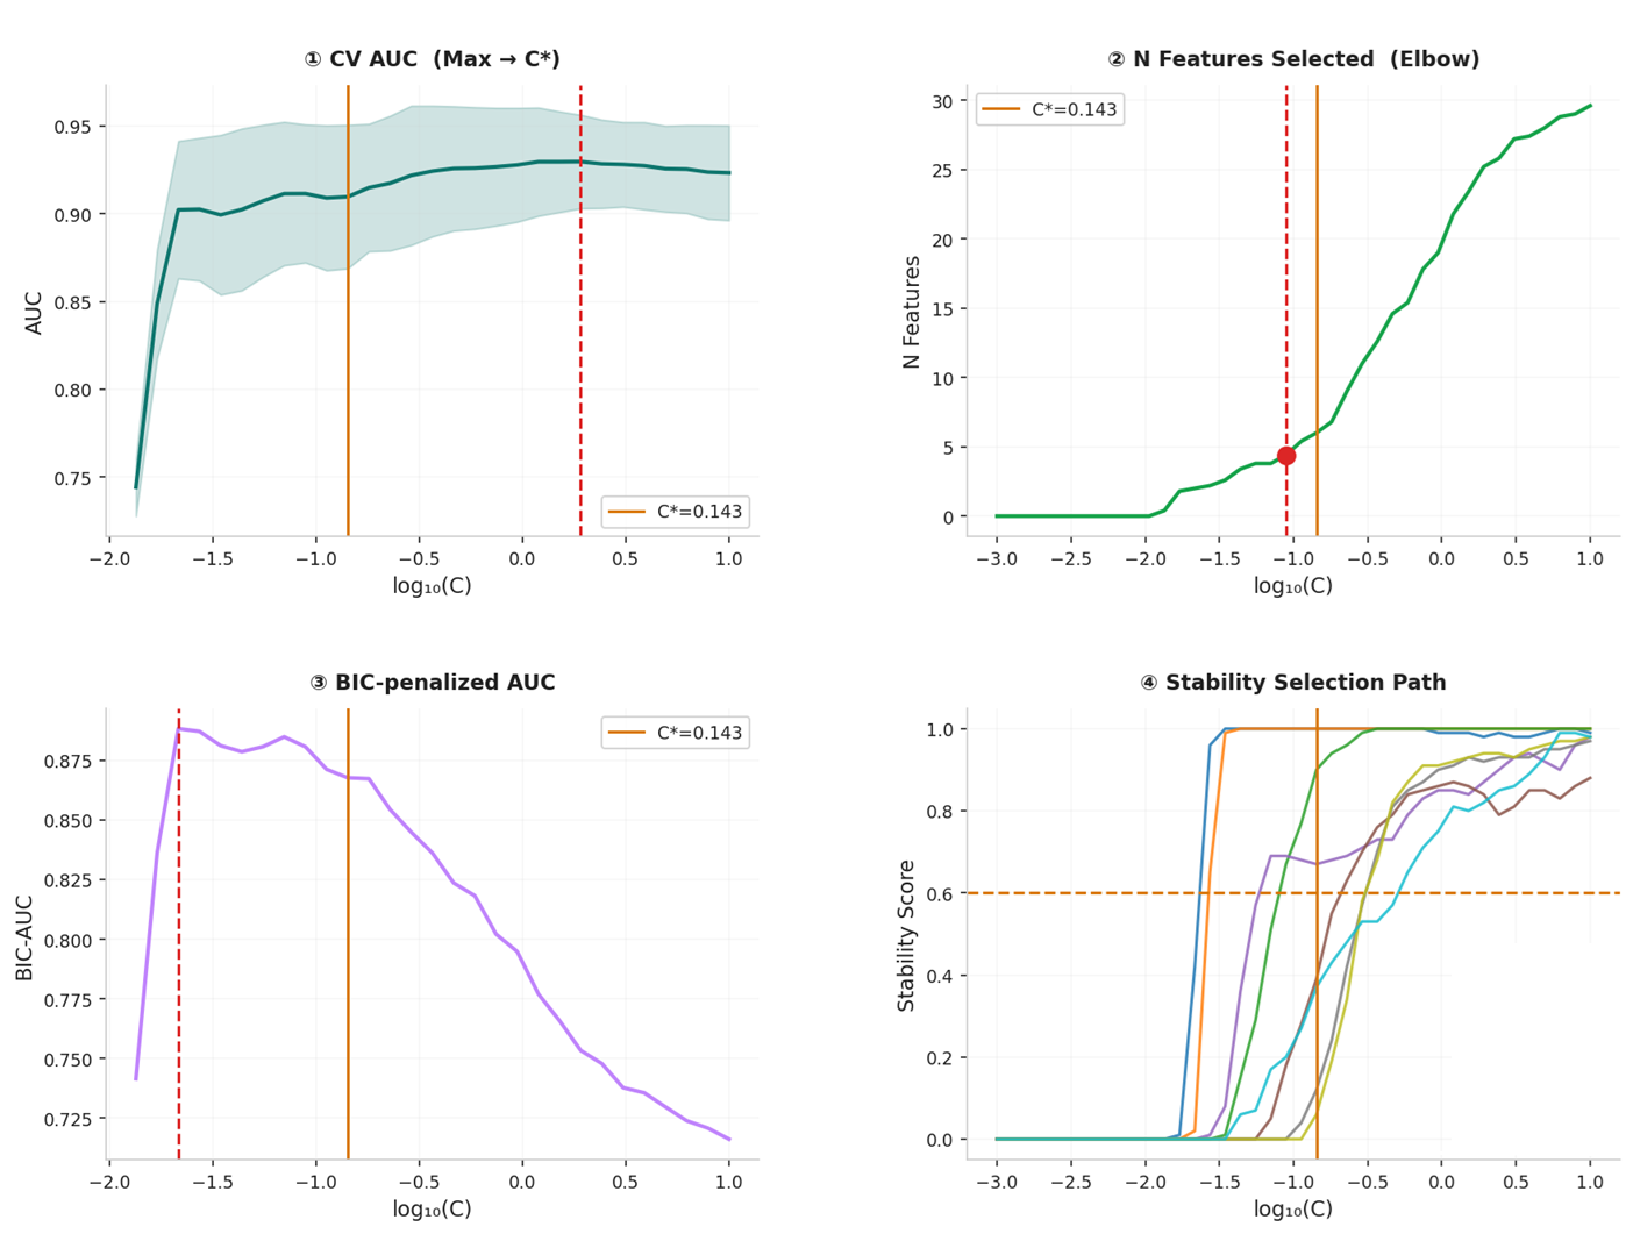
\includegraphics[width=\textwidth]{image/lpro_australian/2_lpro_australian.pdf}
    \end{subfigure}
    
    \caption{Quá trình tối ưu hóa tham số điều chuẩn C trên lưới các tiêu chí trên Australian Credit {
    \newline \small (Trong đó, màu xanh dương = \texttt{CreditScore}, màu cam = \texttt{CreditHistory\_1}, màu xanh lá = \texttt{Income}, tím = \texttt{YearsEmployed}, màu nâu = \texttt{Citizen\_2}, màu xám = \texttt{Age}, màu xanh mạ = \texttt{Employed\_1}, màu xanh trời = \texttt{Debt}; đường ngang đứt nét là ngưỡng \texttt{Threshold = 0.6}})}
    \label{fig:lpro_au}
\end{figure}

\begin{figure}[htbp]
    \centering
    \begin{subfigure}[b]{\textwidth}
        \centering
        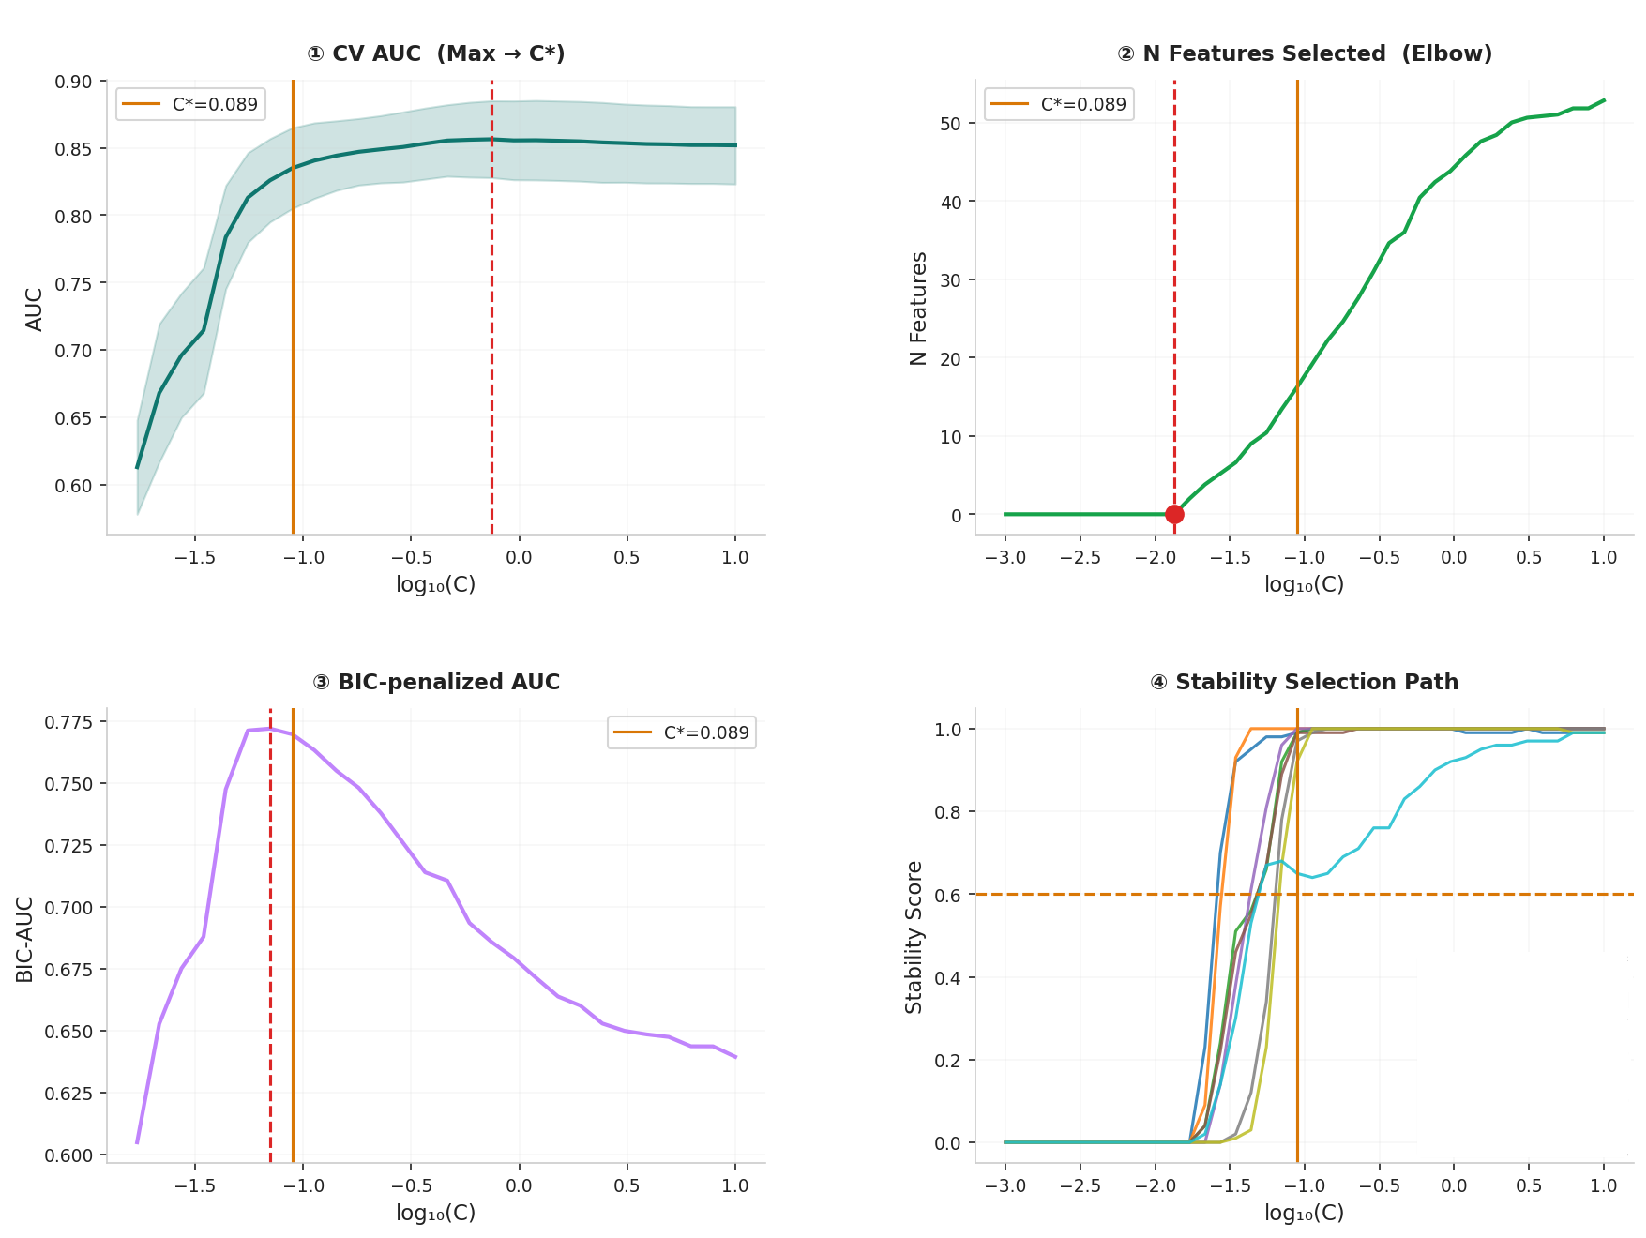
\includegraphics[width=\textwidth]{image/lpro_germany/2_lpro_germany.pdf}
    \end{subfigure}
    
    \caption{Quá trình tối ưu hóa tham số điều chuẩn C trên lưới các tiêu chí trên German Credit {
    \newline \small (Trong đó, màu xanh dương = \texttt{month\_duration}, màu cam = \texttt{age}, màu xanh lá = \texttt{secondary\_obligor\_2.0}, màu tím = \texttt{housing\_1.0}, màu nâu = \texttt{other\_installment\_plans\_1.0}, màu xám = \texttt{status\_account\_3}, màu xanh mạ = \texttt{purpose\_7.0}, màu xanh trời = \texttt{credit\_amount}; đường ngang đứt nét là ngưỡng \texttt{Threshold = 0.6})}}
    \label{fig:lpro_ger}
\end{figure}

\begin{figure}[H]
    \centering
    \begin{subfigure}[b]{\textwidth}
        \centering
        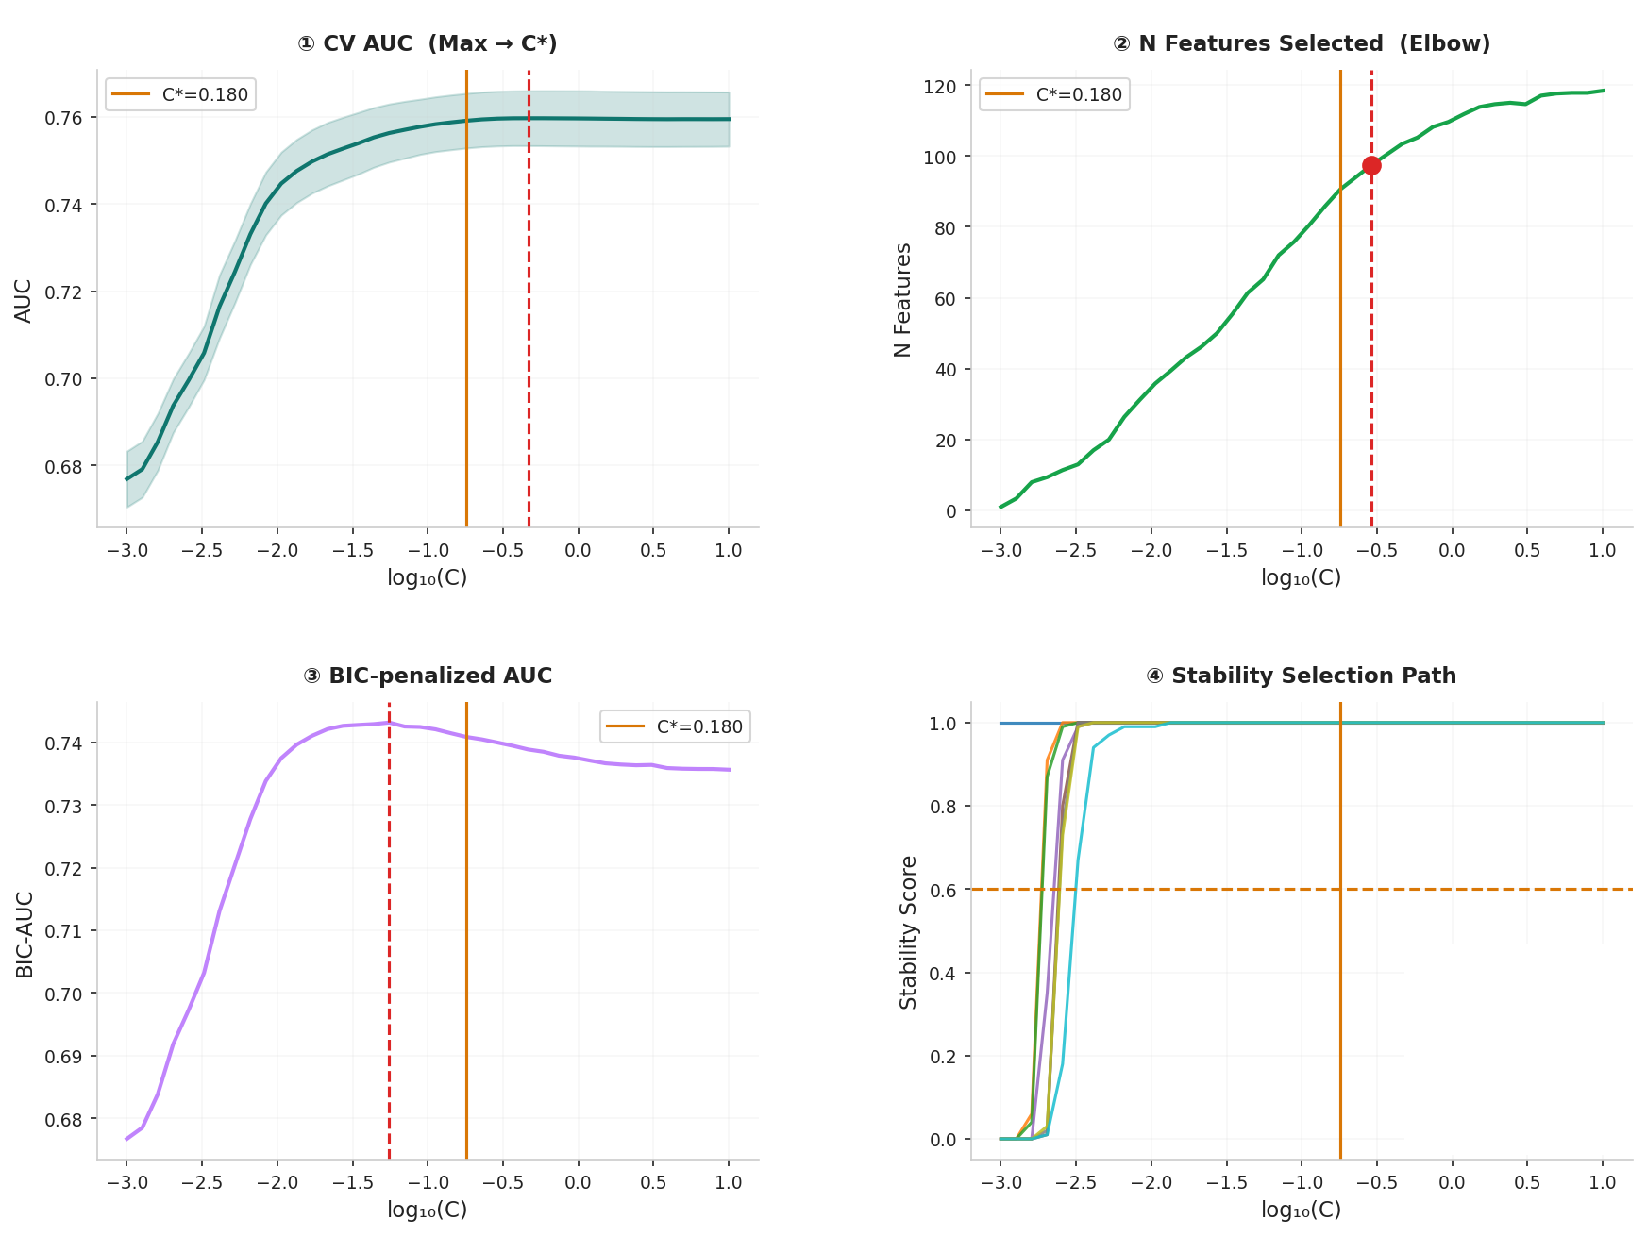
\includegraphics[width=\textwidth]{image/lpro_lending/2_lpro_lending.pdf}
    \end{subfigure}
    
    \caption{Quá trình tối ưu hóa tham số điều chuẩn C trên lưới các tiêu chí trên Lending Club {
    \newline \small (Trong đó, màu xanh dương = \texttt{int\_rate}, màu cam = \texttt{acc\_open\_past\_24mths}, màu xanh lá = \texttt{dti}, tím = \texttt{fico\_range\_low}, màu nâu = \texttt{pub\_rec\_bankruptcies}, màu xám = \texttt{purpose\_2.0}, màu xanh mạ = \texttt{deling\_2yrs}, màu xanh trời = \texttt{mths\_since\_recent\_bc}; đường ngang đứt nét là ngưỡng \texttt{Threshold = 0.6})}}
    \label{fig:lpro_lend}
\end{figure}

\vspace{1em}
Kết quả ba giá trị $C$ ứng viên và $C^*$ tổng hợp trên ba bộ dữ liệu được trình bày tại Bảng \ref{tab:c_selection_criteria}.

\begin{table}[htbp]
    \centering
    \caption{Giá trị tham số $C$ theo từng tiêu chí và $C^*$ tổng hợp}
    \label{tab:c_selection_criteria}
    \renewcommand{\arraystretch}{1.3}
    \begin{tabular}{lcccc}
        \toprule
        \textbf{Bộ dữ liệu} & \textbf{$C_{\text{AUC}}$} & \textbf{$C_{\text{BIC}}$} & \textbf{$C_{\text{elbow}}$} & \textbf{$C^*$} \\ 
        \midrule
        Australian & 1.9145 & 0.0215 & 0.0889 & 0.1425 \\
        German & 0.7444 & 0.0702 & 0.0134 & 0.0889 \\
        Lending Club & 0.4642 & 0.0554 & 0.2894 & 0.1805 \\ 
        \bottomrule
    \end{tabular}
\end{table}

\vspace{1em}
Có thể thấy $C_{\text{AUC}}$ luôn lớn hơn đáng kể so với $C_{\text{BIC}}$ trên cả ba bộ dữ liệu, phản ánh việc tối đa hóa thuần túy AUC có xu hướng giữ lại mô hình kém thưa hơn so với khi có số hạng phạt độ phức tạp. Riêng tại Lending Club, $C_{\text{elbow}}$ lại lớn hơn cả $C_{\text{AUC}}$, cho thấy đường cong số lượng đặc trưng tại bộ dữ liệu này giảm chậm và điểm khuỷu xuất hiện muộn hơn so với hai bộ dữ liệu còn lại, phù hợp với đặc thù không gian đầu vào lớn của Lending Club. Việc lấy trung bình hình học giúp $C^*$ không bị chi phối hoàn toàn bởi tiêu chí cực đoan nhất trong ba ứng viên.

Sau khi xác định $C^*$, một bộ lọc thứ cấp dựa trên Information Value (IV) được áp dụng nhằm loại bỏ các biến có sức phân biệt thực tế quá yếu dù đã được Lasso giữ lại:

\vspace{1em}
\begin{equation}
    \text{IV} = \sum_{i} \left(\text{Dist}_{\text{Event},i} - \text{Dist}_{\text{Non-event},i}\right) \times \ln\left(\frac{\text{Dist}_{\text{Event},i}}{\text{Dist}_{\text{Non-event},i}}\right)
    \label{eq:iv_formula}
\end{equation}

\vspace{1em}
\noindent
với $i$ là chỉ số phân nhóm (\textit{bin}) của biến đặc trưng sau rời rạc hóa. Toàn bộ quy trình ba giai đoạn: xác định $C^*$, trích xuất đặc trưng Lasso, lọc thứ cấp bằng IV được tóm tắt tại Thuật toán \ref{alg:l_pro}.

Trên bộ dữ liệu Australian, Lasso tại $C^* = 0.1425$ chọn được 9 đặc trưng gốc. Sau bộ lọc IV với ngưỡng 0.04, biến \texttt{Gender} bị loại do IV chỉ đạt 0.0001, tập đặc trưng cuối cùng còn 8 biến. Trên bộ dữ liệu German, Lasso tại $C^* = 0.0889$ giữ lại 15 đặc trưng; toàn bộ đều vượt ngưỡng IV 0.05, dẫn đầu là \texttt{secondary\_obligor} ($\text{IV} = 0.6419$), \texttt{other\_installment\_plans} ($\text{IV} = 0.6278$) và \texttt{purpose} ($\text{IV} = 0.6040$), nên không biến nào bị loại. Trên bộ dữ liệu Lending Club, Lasso tại $C^* = 0.1805$ chọn 45 trong 46 biến; bộ lọc IV với ngưỡng 0.03 loại tiếp 18 biến, giữ lại 27 đặc trưng, trong đó \texttt{num\_tl\_op\_past\_12m} ($\text{IV} = 1.1613$), \texttt{inq\_last\_6mths} ($\text{IV} = 0.9930$) và \texttt{num\_actv\_rev\_tl} ($\text{IV} = 0.7156$) là ba biến có sức phân biệt mạnh nhất, phản ánh hành vi tín dụng gần đây và mức độ hoạt động tài khoản là tín hiệu rủi ro chủ đạo của bộ dữ liệu này.

\vspace{1em}
Kết quả sau khi chọn lọc đặc trưng được tổng hợp trong Bảng \ref{tab:lasso_results}.

\begin{table}[htbp]
    \centering
    \caption{Kết quả chọn lọc đặc trưng sau Lasso}
    \label{tab:lasso_results}
    \renewcommand{\arraystretch}{1.3} % Tăng khoảng cách dòng để bảng thoáng hơn
    \begin{tabular}{|l|c|c|c|c|}
        \hline
        \textbf{Bộ dữ liệu} & \textbf{$C^*$} & \textbf{Lasso chọn} & \textbf{Ngưỡng IV} & \textbf{Sau bộ lọc IV} \\ \hline
        Australian & 0.1425 & 9 & 0.04 & 8 \\ \hline
        German & 0.0889 & 15 & 0.05 & 15 \\ \hline
        Lending Club & 0.1805 & 45 & 0.03 & 27 \\ \hline
    \end{tabular}
\end{table}


\vspace{0.5em}
\begin{algorithm}[H]
\caption{Mã giả của quy trình chọn lọc đặc trưng L\_Pro}
\label{alg:l_pro}

\vspace{0.5em}
\textbf{Input:} Tập huấn luyện $(X_{\text{train}}, y_{\text{train}})$ sau S\_Pro; lưới tham số $\mathcal{C} = \{C_1, C_2, \dots, C_{40}\}$ trải đều trên thang $\log_{10}$ từ $10^{-3}$ đến $10^1$; số fold $K = 5$; số bootstrap $B = 100$; ngưỡng ổn định $\tau = 0.6$; ngưỡng IV $\delta$.

\vspace{0.5cm}

\textbf{Output:} Tập đặc trưng cuối cùng $\mathcal{F}^*$ đưa vào K\_Pro.

\begin{tcolorbox}
\begin{algorithmic}[1]
    \Statex \textbf{\textit{// Giai đoạn 1: Xác định $C^*$ tối ưu}}
    \For{mỗi $C \in \mathcal{C}$}
        \State Huấn luyện Logistic-Lasso với penalty $L_1$ và tham số $C$ qua $K$-fold cross-validation
        \State $\text{AUC}_{\text{CV}}(C) \gets$ AUC trung bình trên $K$ fold
        \State $|\mathcal{S}(C)| \gets$ số đặc trưng có $|\hat{\beta}_j| > 0$ trung bình trên $K$ fold
        \State $\text{AUC}_{\text{BIC}}(C) \gets \text{AUC}_{\text{CV}}(C) - \frac{|\mathcal{S}(C)|}{2n}\ln(n)$
        
        \For{$b = 1$ đến $B$} \Comment{Stability Selection}
            \State Lấy mẫu con ngẫu nhiên $50\%$ từ $(X_{\text{train}}, y_{\text{train}})$
            \State Huấn luyện Lasso tại $C$; ghi nhận tập đặc trưng được chọn $\mathcal{S}^{(b)}(C)$
        \EndFor
        
        \State $\Pi_j(C) \gets \frac{1}{B}\sum_{b=1}^{B} \mathbf{1}[j \in \mathcal{S}^{(b)}(C)]$ với mỗi đặc trưng $j$ \Comment{Tần suất chọn}
    \EndFor
    
    \State $C_{\text{AUC}} \gets \arg\max_{C} \text{AUC}_{\text{CV}}(C)$
    \State $C_{\text{BIC}} \gets \arg\max_{C} \text{AUC}_{\text{BIC}}(C)$
    \State $C_{\text{elbow}} \gets$ điểm khuỷu trên đường cong $|\mathcal{S}(C)|$ theo thuật toán Kneedle
    \State $C^* \gets \exp\left(\frac{\ln C_{\text{AUC}} + \ln C_{\text{BIC}} + \ln C_{\text{elbow}}}{3}\right)$, làm tròn về giá trị gần nhất trong $\mathcal{C}$

    \vspace{0.3cm}
    \Statex \textbf{\textit{// Giai đoạn 2: Trích xuất đặc trưng tại $C^*$}}
    \State Huấn luyện Lasso trên toàn bộ $X_{\text{train}}$ tại $C^*$
    \State $\mathcal{S}^* \gets \{j : |\hat{\beta}_j| > 0\}$ \Comment{Tập đặc trưng Lasso sơ bộ}

    \vspace{0.3cm}
    \Statex \textbf{\textit{// Giai đoạn 3: Lọc thứ cấp bằng Information Value}}
    \For{mỗi đặc trưng $j \in \mathcal{S}^*$}
        \State Rời rạc hóa $X_j$ thành các bin; tính $\text{IV}_j = \sum_{i} \left(\text{Dist}_{\text{event},i} - \text{Dist}_{\text{non-event},i}\right) \ln\left(\frac{\text{Dist}_{\text{event},i}}{\text{Dist}_{\text{non-event},i}}\right)$
    \EndFor
    
    \State $\mathcal{F}^* \gets \{j \in \mathcal{S}^* : \text{IV}_j \geq \delta\}$
    \State \textbf{return} $\mathcal{F}^*$
\end{algorithmic}
\end{tcolorbox}
\end{algorithm}
\vspace{0.5em}

\newpage
\subsubsection{Rời rạc hóa dữ liệu (K\_Pro)}
\label{sec: 4.2.5}
\noindent
Như đã trình bày tại Mục \ref{sec: 3.1.3}, việc rời rạc hóa các biến liên tục là điều kiện tiên quyết để mạng Bayes có thể tính toán bảng xác suất có điều kiện thông qua thống kê tần suất, bởi lẽ với biến liên tục mang vô hạn giá trị, mỗi tổ hợp cha-con gần như chỉ xuất hiện đúng một lần trong dữ liệu huấn luyện, khiến ước lượng hợp lý cực đại trở nên vô nghĩa do thiếu quan sát lặp lại. Tuy nhiên, áp dụng trực tiếp thuật toán K-means theo Công thức \ref{eq: 3.3} lên các biến tài chính nguyên gốc - vốn có phân phối lệch nặng do đặc tính của dữ liệu tín dụng (thu nhập, dư nợ, số dư tín dụng thường tập trung dày ở mức thấp và kéo đuôi dài về phía giá trị cao) - sẽ dẫn đến hiện tượng các cụm bị chi phối bởi một vài điểm ngoại lai cực đoan, khiến phần lớn quan sát bị dồn vào một hoặc hai bin trong khi các bin còn lại gần như trống.

Để khắc phục hạn chế này, quy trình thực nghiệm bổ sung một bước biến đổi phân phối trước khi đưa dữ liệu vào K-means theo Thuật toán \ref{alg:kmeans_discretization} đã trình bày tại Mục \ref{sec: 3.1.3}. Bước bổ sung này áp dụng phép biến đổi lũy thừa Yeo-Johnson, được định nghĩa theo bốn trường hợp tùy vào dấu của giá trị gốc $x$ và tham số hình dạng $\lambda$:
\begin{equation}
\psi(x; \lambda) =
\begin{cases}
\dfrac{(x+1)^{\lambda} - 1}{\lambda}, & \lambda \neq 0,\ x \geq 0 \\[8pt]
\ln(x+1), & \lambda = 0,\ x \geq 0 \\[8pt]
-\dfrac{(-x+1)^{2-\lambda} - 1}{2-\lambda}, & \lambda \neq 2,\ x < 0 \\[8pt]
-\ln(-x+1), & \lambda = 2,\ x < 0
\end{cases}
\label{eq:yeo_johnson}
\end{equation}
trong đó tham số $\lambda$ được ước lượng bằng phương pháp hợp lý cực đại trên tập huấn luyện, sao cho phân phối của $\psi(x;\lambda)$ tiệm cận gần nhất với phân phối chuẩn \citep{yeo2000}. Hai nhánh đầu xử lý giá trị không âm theo cùng cơ chế với biến đổi Box-Cox cộng thêm hằng số dịch chuyển, trong khi hai nhánh sau mở rộng công thức sang miền giá trị âm bằng phép phản chiếu qua gốc tọa độ, qua đó khắc phục được hạn chế cố hữu của Box-Cox vốn chỉ xác định trên miền dương. Phép biến đổi này được lựa chọn vì khả năng xử lý cả giá trị âm và bằng $0$, vốn xuất hiện phổ biến trong các biến như chênh lệch nợ hoặc số tháng kể từ sự kiện gần nhất, đồng thời san phẳng độ lệch và giảm ảnh hưởng của giá trị ngoại lai mà không làm mất thông tin như các kỹ thuật cắt ngưỡng (capping) truyền thống.

Đối với bộ dữ liệu Lending Club, do thang đo giữa các biến chênh lệch rất lớn - chẳng hạn \texttt{loan\_amnt} tính bằng nghìn đô-la trong khi \texttt{dti} tính theo phần trăm - một bước chuẩn hóa \texttt{StandardScaler} được thực hiện trước Yeo-Johnson nhằm đưa các biến về cùng thang đo, tránh tình trạng biến có phương sai lớn lấn át quá trình ước lượng tham số biến đổi của các biến còn lại. Sau khi dữ liệu được chuẩn hóa phân phối, thuật toán K-means theo Thuật toán \ref{alg:kmeans_discretization} được áp dụng trên không gian đã biến đổi với số bin cố định $k = 4$ cho toàn bộ các biến liên tục. Số bin $k = 4$ được lựa chọn nhằm cân bằng giữa hai mục tiêu đối nghịch: duy trì đủ độ phân giải để các bin phản ánh được sự khác biệt về rủi ro tín dụng giữa các mức giá trị, đồng thời tránh tình trạng phân mảnh quá mức khiến một số tổ hợp trạng thái cha-con trong mạng Bayes rơi vào vùng dữ liệu thưa. Ranh giới của từng bin sau đó được ánh xạ ngược về thang giá trị gốc bằng cách lấy giá trị nhỏ nhất và lớn nhất thực tế của các quan sát rơi vào bin đó trên tập huấn luyện, đảm bảo các khoảng giá trị được báo cáo phản ánh đúng phân phối dữ liệu chứ không phải ranh giới lý thuyết của cụm trong không gian đã biến đổi.

Kết quả rời rạc hóa trên bộ dữ liệu Australian được trình bày tại Bảng \ref{tab:australian_features_kpro}. Biến \texttt{Debt} được chia thành bốn khoảng $[0.00; 1.08)$, $[1.08; 3.29)$, $[3.29; 8.00)$ và $[8.00; 28.00]$, trong đó tỷ lệ vỡ nợ giảm dần từ $54.78\%$ ở bin thấp nhất xuống còn $32.41\%$ ở bin cao nhất - một xu hướng có phần phản trực giác nếu xét theo logic thông thường rằng nợ càng cao thì rủi ro càng lớn, song có thể giải thích bởi việc các khoản nợ lớn thường gắn với hồ sơ tín dụng đã được thẩm định kỹ và có tài sản đảm bảo tương ứng. Biến \texttt{YearsEmployed} thể hiện quan hệ đơn điệu rõ ràng hơn, với tỷ lệ vỡ nợ giảm mạnh từ $72.16\%$ ở nhóm có thời gian làm việc dưới $0.54$ năm xuống còn $19.23\%$ ở nhóm trên $4.33$ năm, phản ánh đúng trực giác rằng thâm niên công việc ổn định tương quan nghịch với rủi ro tín dụng. Biến \texttt{CreditScore} cho thấy mức phân tách event rate mạnh nhất trong số các biến liên tục của bộ dữ liệu này, từ $71.61\%$ tại bin thấp nhất xuống chỉ còn $9.18\%$ tại bin cao nhất, củng cố vai trò của biến này như một chỉ báo rủi ro hàng đầu.

Kết quả rời rạc hóa trên bộ dữ liệu German được trình bày tại Bảng \ref{tab:german_features_kpro}. Trên bộ dữ liệu German, biến \texttt{month\_duration} - thời hạn vay tính theo tháng - biểu hiện quan hệ đồng biến với rủi ro vỡ nợ, tăng từ $14.00\%$ ở nhóm vay ngắn hạn (4-9 tháng) lên $70.79\%$ ở nhóm vay dài hạn (31-60 tháng), phù hợp với lý thuyết tài chính rằng kỳ hạn vay càng dài thì rủi ro tín dụng tích lũy càng lớn do thời gian phơi nhiễm trước các cú sốc thu nhập kéo dài hơn. Biến \texttt{age} cho thấy xu hướng ngược lại, với tỷ lệ vỡ nợ giảm từ $57.38\%$ ở nhóm tuổi 19-25 xuống còn $32.74\%$ ở nhóm trên 43 tuổi, phản ánh sự ổn định tài chính tăng dần theo độ tuổi. Biến \texttt{credit\_amount} không thể hiện quan hệ đơn điệu, dao động trong khoảng $43.65\%$-$62.15\%$ qua các bin, cho thấy quy mô khoản vay đơn thuần không phải là yếu tố quyết định mạnh đến khả năng vỡ nợ trên bộ dữ liệu này nếu tách biệt khỏi các biến khác.

Kết quả rời rạc hóa trên bộ dữ liệu Lending Club được trình bày tại Bảng \ref{tab:lending_club_features_kpro}. Trên bộ dữ liệu Lending Club, biến \texttt{int\_rate} - lãi suất cho vay - thể hiện quan hệ đồng biến rõ rệt và mạnh nhất trong toàn bộ các biến liên tục được khảo sát, với tỷ lệ vỡ nợ tăng từ $22.54\%$ ở bin lãi suất thấp nhất ($6.00\%$-$10.80\%$) lên đến $69.09\%$ ở bin lãi suất cao nhất ($19.59\%$-$26.06\%$), nhất quán với cơ chế định giá rủi ro của các nền tảng cho vay ngang hàng, theo đó lãi suất được ấn định cao hơn cho các khoản vay được đánh giá rủi ro lớn hơn ngay từ khâu thẩm định ban đầu. Biến \texttt{dti} (tỷ lệ nợ trên thu nhập) cũng cho thấy xu hướng đồng biến nhất quán, từ $38.02\%$ lên $56.03\%$ qua bốn bin, phù hợp với kỳ vọng rằng gánh nặng nợ tương đối cao so với thu nhập làm suy giảm khả năng trả nợ. Ngược lại, các biến phản ánh độ sâu lịch sử tín dụng như \texttt{mo\_sin\_rcnt\_tl} (số tháng kể từ tài khoản tín dụng gần nhất được mở) và \texttt{mths\_since\_recent\_bc} lại thể hiện quan hệ nghịch biến ở bin cao nhất, với tỷ lệ vỡ nợ giảm xuống còn $35.88\%$ và $41.51\%$ tương ứng - cho thấy khách hàng không mở tài khoản tín dụng mới trong thời gian dài có xu hướng ổn định tài chính hơn. Đáng chú ý, biến \texttt{revol\_util} tại bộ dữ liệu này xuất hiện một bin chỉ chứa duy nhất một quan sát với tỷ lệ vỡ nợ $100\%$, một hiện tượng điển hình của rời rạc hóa dựa trên K-means khi tồn tại điểm ngoại lai cực đoan tách biệt hẳn khỏi phần còn lại của phân phối dù đã qua phép biến đổi Yeo-Johnson.

Toàn bộ quy trình \textit{power-transform} và \textit{K-means discretization} được \textit{fit} (ước lượng tham số) duy nhất trên tập huấn luyện, sau đó áp dụng \textit{transform} tương ứng lên tập kiểm tra nhằm tránh rò rỉ thông tin từ tập kiểm tra vào quá trình xác định ranh giới bin.

% ===== BẢNG 4.5: Australian (longtable) =====
\renewcommand{\arraystretch}{1.4}
\begin{longtable}{V{2.9cm}D{9.3cm}S{2.4cm}}
    \caption{Mô tả các đặc trưng đã chọn của bộ dữ liệu Australian sau K\_Pro}
    \label{tab:australian_features_kpro} \\
 
    \toprule
    \textbf{Tên biến} & \textbf{Mô tả} & \textbf{States} \\
    \midrule
    \endfirsthead
 
    \multicolumn{3}{c}%
    {{\bfseries \tablename\ \thetable{} (tiếp theo)}} \\
    \toprule
    \textbf{Tên biến} & \textbf{Mô tả} & \textbf{States} \\
    \midrule
    \endhead
 
    \midrule
    \multicolumn{3}{r}{{Tiếp tục ở trang sau...}} \\
    \endfoot
 
    \bottomrule
    \endlastfoot
 
    \varname{CreditHistory} & Lịch sử tín dụng trước đó của người nộp đơn \newline Không, có & 0, 1 \\
    \varname{CreditScore} & Điểm tín dụng của người nộp đơn \newline $(0; 1]$, $(1; 2]$, $(2; 4]$, $(4; 40]$ & 0, 1, 2, 3 \\
    \varname{Employed} & Tình trạng đang đi làm tại thời điểm nộp đơn \newline Không, có & 0, 1 \\
    \varname{YearsEmployed} & Số năm làm việc tại nơi công tác hiện tại \newline $(0.00; 0.54]$, $(0.54; 1.96]$, $(1.96; 4.33]$, $(4.33; 28.50]$ & 0, 1, 2, 3 \\
    \varname{Income} & Thu nhập của người nộp đơn \newline $(1; 5]$, $(5; 51]$, $(51; 679]$, $(679; 51101]$ & 0, 1, 2, 3 \\
    \varname{Debt} & Tổng dư nợ hiện tại của người nộp đơn \newline $(0.00; 1.08]$, $(1.08; 3.29]$, $(3.29; 8.00]$, $(8.00; 28.00]$ & 0, 1, 2, 3 \\
    \varname{Age} & Tuổi của người nộp đơn \newline $(13.75; 21.67]$, $(21.67; 29.17]$, $(29.17; 41.00]$, $(41.00; 80.25]$ & 0, 1, 2, 3 \\
    \varname{Citizen} & Tình trạng quốc tịch/cư trú của người nộp đơn & 1, 2, 3 \\
    \varname{target} & Trạng thái phê duyệt hồ sơ tín dụng \newline Vỡ nợ, không vỡ nợ & 0, 1 \\
 
\end{longtable}
 
% ===== BẢNG 4.6: German Credit (longtable) =====
\renewcommand{\arraystretch}{1.4}
\begin{longtable}{V{2.9cm}D{9.3cm}S{2.4cm}}
    \caption{Mô tả các đặc trưng đã chọn của bộ dữ liệu German Credit sau K\_Pro}
    \label{tab:german_features_kpro} \\
 
    \toprule
    \textbf{Tên biến} & \textbf{Mô tả} & \textbf{States} \\
    \midrule
    \endfirsthead
 
    \multicolumn{3}{c}%
    {{\bfseries \tablename\ \thetable{} (tiếp theo)}} \\
    \toprule
    \textbf{Tên biến} & \textbf{Mô tả} & \textbf{States} \\
    \midrule
    \endhead
 
    \midrule
    \multicolumn{3}{r}{{Tiếp tục ở trang sau...}} \\
    \endfoot
 
    \bottomrule
    \endlastfoot
 
    \varname{status_account} & Tình trạng tài khoản vãng lai của khách hàng tại ngân hàng \newline $< 0$ DM, $0 \leq \dots < 200$ DM, $\geq 200$ DM, no checking account & 0, 1, 2, 3 \\
    \varname{month_duration} & Thời hạn vay tính theo tháng \newline $(4; 9]$, $(9; 17]$, $(17; 31]$, $(31; 60]$ & 0, 1, 2, 3 \\
    \varname{credit_history} & Lịch sử tín dụng của khách hàng \newline No credits taken/all credits paid back duly, all credits at this bank paid back duly, existing credits paid back duly till now, delay in paying off in the past, critical account/other credits existing & 0, 1, 2, 3, 4 \\
    \varname{purpose} & Mục đích vay \newline Car (new), car (used), furniture/equipment, radio/television, domestic appliances, repairs, education, retraining, business, others & 0, 1, 2, 3, 4, 5, 6, 7, 8, 9 \\
    \varname{credit_amount} & Số tiền vay \newline $(250; 1068]$, $(1068; 2279]$, $(2279; 5433]$, $(5433; 18424]$ & 0, 1, 2, 3 \\
    \varname{status_and_sex} & Tình trạng hôn nhân và giới tính \newline Male: divorced/separated, female: divorced/separated/married, male: single, male: married/widowed & 0, 1, 2, 3 \\
    \varname{secondary_obligor} & Người bảo lãnh hoặc đồng vay \newline None, co-applicant, guarantor & 0, 1, 2 \\
    \varname{residence_since} & Số năm cư trú tại nơi ở hiện tại & 1, 2, 3, 4 \\
    \varname{collateral} & Tài sản đảm bảo \newline Real estate, building society savings agreement/life insurance, car or other, unknown/no property & 0, 1, 2, 3 \\
    \varname{age} & Tuổi của khách hàng \newline $(19; 25]$, $(25; 32]$, $(32; 43]$, $(43; 75]$ & 0, 1, 2, 3 \\
    \varname{other_installment_plans} & Các khoản trả góp khác đang có \newline Bank, stores, none & 0, 1, 2 \\
    \varname{housing} & Tình trạng nhà ở \newline Rent, own, for free & 0, 1, 2 \\
    \varname{n_credits} & Số khoản tín dụng hiện có tại ngân hàng này & 1, 2, 3, 4 \\
    \varname{job} & Tình trạng nghề nghiệp \newline Unemployed/unskilled non-resident, unskilled resident, skilled employee/official, management/self-employed/highly qualified & 0, 1, 2, 3 \\
    \varname{is_foreign_worker} & Tình trạng lao động nước ngoài \newline Yes, no & 0, 1 \\
    \varname{target} & Tình trạng tín dụng của khách hàng \newline Good, bad & 0, 1 \\
 
\end{longtable}
 
% ===== BẢNG 4.7: Lending Club (longtable) =====
\renewcommand{\arraystretch}{1.3}
\begin{longtable}{V{2.6cm}D{9.0cm}S{3.0cm}}
    \caption{Mô tả các đặc trưng đã chọn của bộ dữ liệu Lending Club 2007-2014 sau K\_Pro}
    \label{tab:lending_club_features_kpro} \\
 
    \toprule
    \textbf{Tên biến} & \textbf{Mô tả} & \textbf{States} \\
    \midrule
    \endfirsthead
 
    \multicolumn{3}{c}%
    {{\bfseries \tablename\ \thetable{} (tiếp theo)}} \\
    \toprule
    \textbf{Tên biến} & \textbf{Mô tả} & \textbf{States} \\
    \midrule
    \endhead
 
    \midrule
    \multicolumn{3}{r}{{Tiếp tục ở trang sau...}} \\
    \endfoot
 
    \bottomrule
    \endlastfoot
 
    \varname{term} & Số tháng trả nợ của khoản vay \newline 36 months, 60 months & 0, 1 \\
 
    \varname{grade} & Hạng tín dụng do Lending Club xếp loại cho khoản vay (A đến G) & 0, 1, 2, 3, 4, 5, 6 \\
 
    \varname{emp_length} & Số năm làm việc của người vay \newline Unknown, $< 1$ year, $1$ year, $2$ years, $3$ years, $4$ years, $5$ years, $6$ years, $7$ years, $8$ years, $9$ years, $10+$ years & 0, 1, 2, 3, 4, 5, 6, 7, 8, 9, 10, 11 \\
 
    \varname{verification_status} & Tình trạng xác minh nguồn thu nhập của người vay \newline Not Verified, Verified, Source Verified & 0, 1, 2 \\
 
    \varname{home_ownership} & Tình trạng sở hữu nhà của người vay \newline MORTGAGE, OTHER, OWN, RENT & 0, 1, 2, 3 \\
 
    \varname{purpose} & Mục đích vay do người vay khai báo \newline car, credit\_card, debt\_consolidation, home\_improvement, house, major\_purchase, medical, moving, other, renewable\_energy, small\_business, vacation, wedding & 0, 1, 2, 3, 4, 5, 6, 7, 8, 9, 10, 11, 12 \\
 
    \varname{debt_settlement_flag} & Cho biết hồ sơ vay có đang nằm trong chương trình tái cơ cấu nợ (debt settlement) hay không & 0, 1 \\
 
    \varname{loan_amnt} & Số tiền vay được người vay đề nghị tại thời điểm nộp đơn \newline $(1000.00; 7713.40]$, $(7713.40; 13649.90]$, $(13649.90; 22325.00]$, $(22325.00; 35000.00]$ & 0, 1, 2, 3 \\
 
    \varname{annual_inc} & Thu nhập hàng năm tự khai báo của người vay \newline $(3000.00; 43264.00]$, $(43264.00; 66296.67]$, $(66296.67; 106453.62]$, $(106453.62; 2000000.00]$ & 0, 1, 2, 3 \\
 
    \varname{int_rate} & Lãi suất của khoản vay \newline $(6.00; 10.80]$, $(10.80; 15.11]$, $(15.11; 19.59]$, $(19.59; 26.06]$ & 0, 1, 2, 3 \\
 
    \varname{dti} & Tỷ lệ tổng nợ hàng tháng (không tính khoản vay này và thế chấp) trên thu nhập hàng tháng tự khai báo \newline $(0.00; 11.50]$, $(11.50; 18.53]$, $(18.53; 25.82]$, $(25.82; 39.99]$ & 0, 1, 2, 3 \\
 
    \varname{fico_range_low} & Cận dưới khoảng điểm FICO của người vay tại thời điểm khởi tạo khoản vay \newline $(660.00; 675.58]$, $(675.58; 695.41]$, $(695.41; 726.54]$, $(726.54; 845.00]$ & 0, 1, 2, 3 \\
 
    \varname{revol_util} & Tỷ lệ sử dụng hạn mức tín dụng quay vòng so với tổng hạn mức được cấp \newline $(0.00; 45.45]$, $(45.45; 71.26]$, $(71.26; 366.60]$, $= 366.60$ & 0, 1, 2, 3 \\
 
    \varname{tot_cur_bal} & Tổng số dư hiện tại trên toàn bộ các tài khoản tín dụng \newline $(0.00; 48110.00]$, $(48110.00; 115417.00]$, $(115417.00; 246217.00]$, $(246217.00; 2179304.00]$ & 0, 1, 2, 3 \\
 
    \varname{bc_open_to_buy} & Hạn mức tín dụng còn khả dụng trên các tài khoản thẻ ngân hàng \newline $(0.00; 1824.00]$, $(1824.00; 4873.00]$, $(4873.00; 11413.00]$, $(11413.00; 168099.00]$ & 0, 1, 2, 3 \\
 
    \varname{mo_sin_rcnt_rev_tl_op} & Số tháng kể từ khi tài khoản tín dụng quay vòng gần nhất được mở \newline $(0.00; 4.54]$, $(4.54; 9.99]$, $(9.99; 21.11]$, $(21.11; 217.00]$ & 0, 1, 2, 3 \\
 
    \varname{mo_sin_rcnt_tl} & Số tháng kể từ khi tài khoản tín dụng gần nhất được mở \newline $(0.00; 3.44]$, $(3.44; 7.13]$, $(7.13; 14.05]$, $(14.05; 102.00]$ & 0, 1, 2, 3 \\
 
    \varname{mths_since_recent_bc} & Số tháng kể từ khi tài khoản thẻ ngân hàng gần nhất được mở \newline $(0.00; 8.25]$, $(8.25; 18.03]$, $(18.03; 38.10]$, $(38.10; 521.00]$ & 0, 1, 2, 3 \\
 
    \varname{mths_since_recent_inq} & Số tháng kể từ lần truy vấn tín dụng gần nhất \newline $(0.00; 2.60]$, $(2.60; 6.34]$, $(6.34; 12.26]$, $(12.26; 24.00]$ & 0, 1, 2, 3 \\
 
    \varname{inq_last_6mths} & Số lần truy vấn tín dụng trong 6 tháng gần nhất \newline $(0.00; 0.41]$, $(0.41; 1.37]$, $(1.37; 2.54]$, $(2.54; 6.00]$ & 0, 1, 2, 3 \\
 
    \varname{acc_open_past_24mths} & Số tài khoản tín dụng được mở trong 24 tháng gần nhất \newline $(0.00; 3.33]$, $(3.33; 6.03]$, $(6.03; 9.38]$, $(9.38; 50.00]$ & 0, 1, 2, 3 \\
 
    \varname{mort_acc} & Số tài khoản thế chấp (mortgage) hiện có \newline $(0.00; 1.09]$, $(1.09; 3.23]$, $(3.23; 6.03]$, $(6.03; 24.00]$ & 0, 1, 2, 3 \\
 
    \varname{num_accts_ever_120_pd} & Số tài khoản từng quá hạn từ 120 ngày trở lên \newline $(0.00; 0.08]$, $(0.08; 0.30]$, $(0.30; 0.71]$, $(0.71; 21.00]$ & 0, 1, 2, 3 \\
 
    \varname{num_actv_rev_tl} & Số tài khoản tín dụng quay vòng đang hoạt động \newline $(0.00; 3.64]$, $(3.64; 6.21]$, $(6.21; 10.11]$, $(10.11; 31.00]$ & 0, 1, 2, 3 \\
 
    \varname{num_bc_tl} & Số tài khoản thẻ ngân hàng hiện có \newline $(1.00; 5.49]$, $(5.49; 9.18]$, $(9.18; 14.42]$, $(14.42; 44.00]$ & 0, 1, 2, 3 \\
 
    \varname{num_il_tl} & Số tài khoản tín dụng trả góp hiện có \newline $(1.00; 4.29]$, $(4.29; 8.29]$, $(8.29; 15.31]$, $(15.31; 97.00]$ & 0, 1, 2, 3 \\
 
    \varname{num_tl_op_past_12m} & Số tài khoản tín dụng được mở trong 12 tháng gần nhất \newline $(0.00; 1.42]$, $(1.42; 3.16]$, $(3.16; 5.46]$, $(5.46; 17.00]$ & 0, 1, 2, 3 \\
 
    \varname{target} & Trạng thái vỡ nợ của khoản vay \newline Không, có & 0, 1 \\
 
\end{longtable}

\subsection{Xây dựng mạng Bayes và dự đoán (BN\_Pro)}
\subsubsection{Xây dựng cấu trúc mạng và dự đoán}
\label{sec: 4.3.1}
\noindent
Thư viện cốt lõi cho xây dựng và suy luận mạng Bayes là pgmpy, sử dụng các lớp DiscreteBayesianNetwork, HillClimbSearch (thuật toán Tabu Search, cấu trúc DAG được học bằng Tabu Search tối ưu điểm số BIC cho dữ liệu rời rạc (bic-d), với 50 lần huấn luyện độc lập (N\_RUNS = 50), mỗi lần khởi tạo từ một DAG ngẫu nhiên khác nhau (random restart) để tránh cực trị địa phương.

\noindent
Cấu hình: 
\begin{itemize}
    \item Số lần huấn luyện: N\_RUNS = 50 
    \item Bộ nhớ Tabu (tabu\_length) = 100 hoạt động như một bộ nhớ ngắn hạn lưu trữ các hành động thêm, xóa, đảo ngược cạnh mà thuật toán vừa mới thực hiện trong 100 bước gần nhất. 
    \item Bậc vào tối đa mỗi node (max\_indegree) = 5 là số mũi tên tối đa hướng trực tiếp đi vào một nút đồng nghĩa với việc số nút cha tối đa của nút đó, nhằm kiểm soát kích thước bảng CPT.
    \item Số bước tìm kiếm tối đa mỗi run (max\_iter) = 1000.
    \item Xác suất sinh cạnh ban đầu (edge\_prob) = 0.3 (đặt xác suất thấp $\leq 0.5$ để tránh đồ thị sinh ra sẽ rất dày đặc, các nút kết nối chằng chịt với nhau làm tăng độ phức tạp của đồ thị. Đối với một đồ thị có hướng không chu trình gồm $n$ nút , số lượng cặp nút có thể thiết lặp liên kết là $M_{max} = \binom{n}{2} = \frac{n(n-1)}{2}$, số lượng cạnh trung bình xuất hiện trên toàn bộ đồ thị sinh ban đầu là 
    \begin{equation}
        E(M) = edge\_prob \times M_{max} = edge\_prob \times \frac{n(n-1)}{2}
    \end{equation}    
    
\end{itemize}


Sau 50 lần chạy, DAG có điểm BIC cao nhất (ít âm nhất) được chọn làm cấu trúc cuối cùng. Bảng \ref{tab:result_dag} tổng hợp kết quả học cấu trúc trên ba bộ dữ liệu.
\begin{table}[htbp]
\centering
\caption{Kết quả tối ưu cấu trúc DAG bằng thuật toán tìm kiếm Tabu}
\label{tab:result_dag}

\renewcommand{\arraystretch}{1.3}

\begin{tabular}{|>{\centering\arraybackslash}p{2.3cm}|
>{\centering\arraybackslash}p{2.2cm}|
>{\centering\arraybackslash}p{2cm}|
>{\centering\arraybackslash}p{1.7cm}|
>{\centering\arraybackslash}p{2cm}|
>{\centering\arraybackslash}p{3.8cm}|}
\hline

\rowcolor{gray!20}
\textcolor{black}{\textbf{Bộ dữ liệu}} &
\textcolor{black}{\textbf{BIC tốt nhất}} &
\textcolor{black}{\textbf{Run tốt nhất}} &
\textcolor{black}{\textbf{Số node}} &
\textcolor{black}{\textbf{Số cạnh}} &
\textcolor{black}{\textbf{Dao động BIC giữa các run}} \\

\hline

Australian Credit
& -3343.32
& 15
& 9
& 10 
& $\approx$ 44 đơn vị 

(-3387 → -3343)\\

\hline

German Credit
& -14755.32
& 20
& 16
& 18 
& $\approx$ 114 đơn vị 

(-14869 → -14755)\\

\hline

Lending Club
& -725970.15
& 14
& 28
& 58 
& $\approx$ 3.500 đơn vị 

(-729492 → -725970)\\

\hline
\end{tabular}
\end{table} 

% ==========================================
% KHỐI HÌNH 1: Chứa Australian và German
% ==========================================
\begin{figure}[H]
    \centering

     % --- HÀNG 1: Australian Credit ---
    \begin{subfigure}[b]{0.8\textwidth} % Giảm nhẹ xuống 0.8 để 2 hình chắc chắn vừa 1 trang
        \centering
        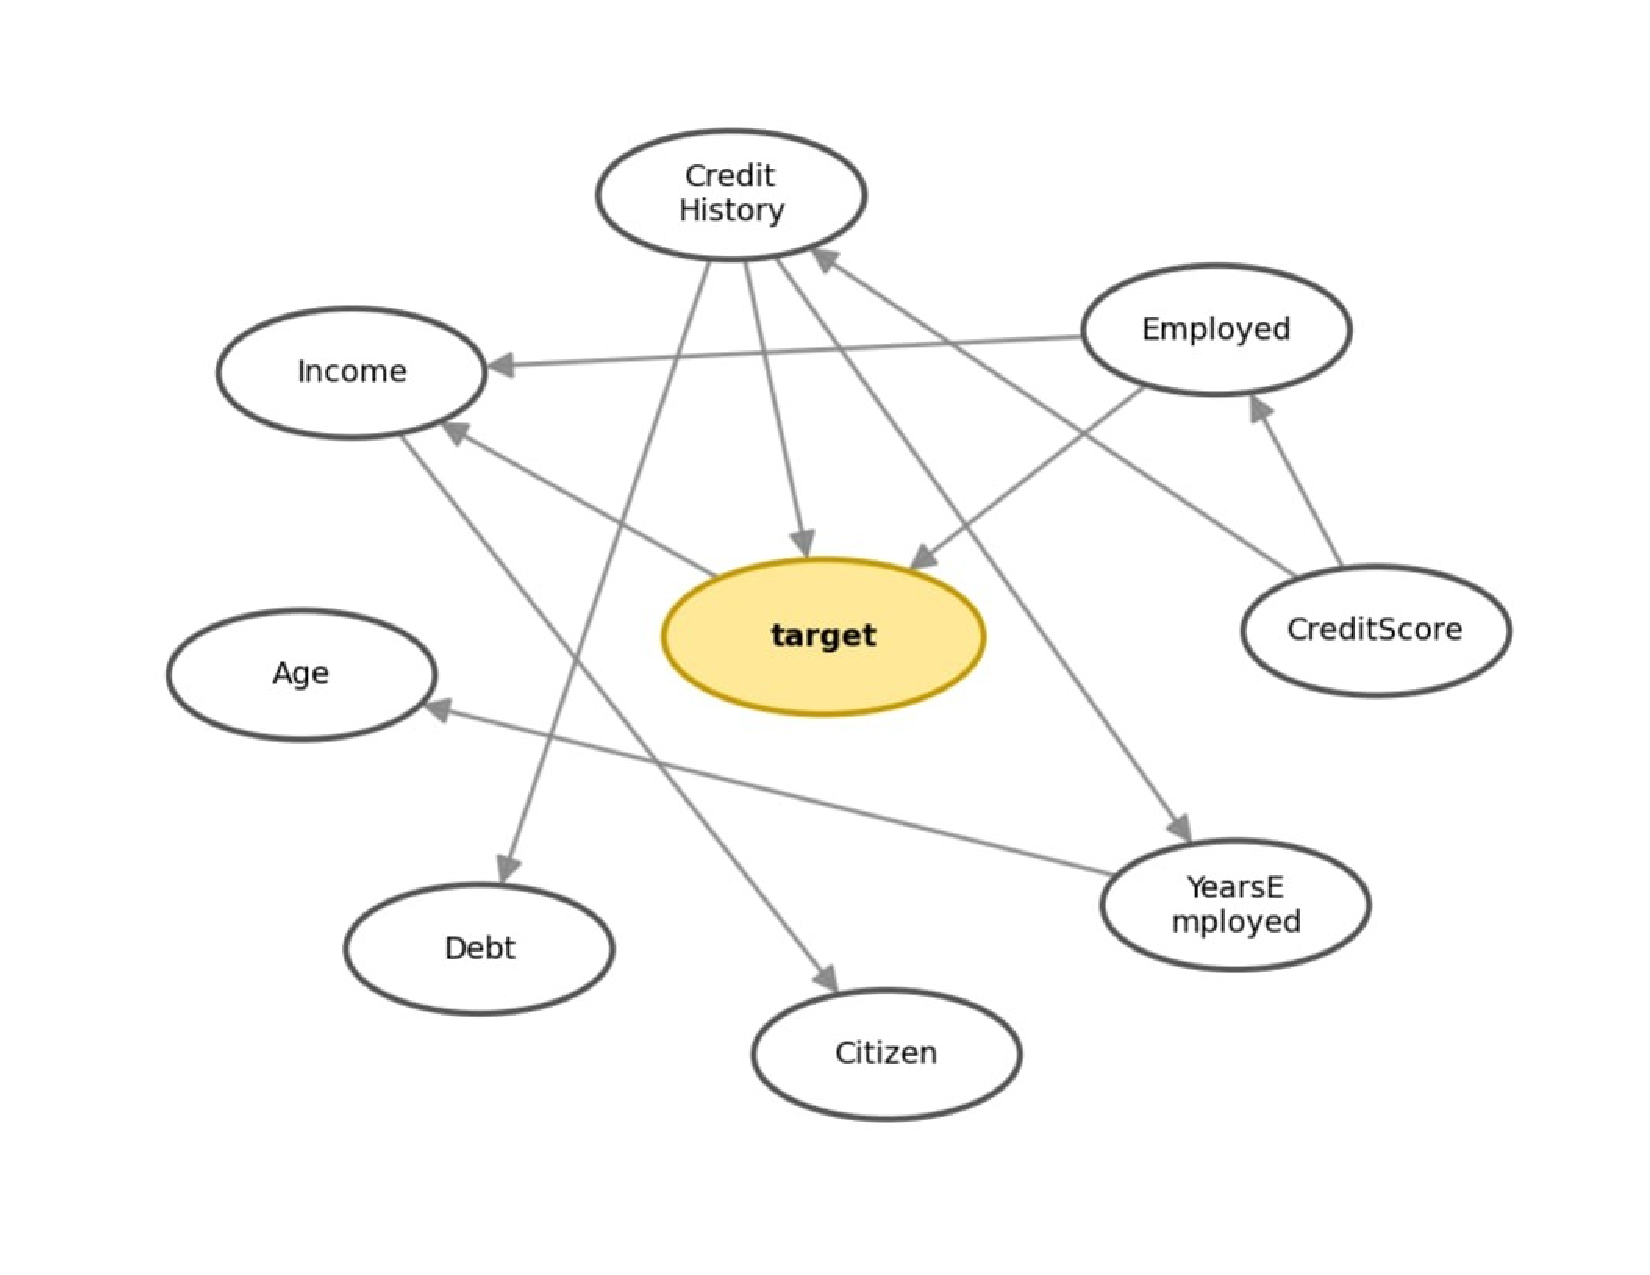
\includegraphics[width=\textwidth,
        height=0.35\textheight,
        trim=2.5cm 2.5cm 2cm 2cm,
        clip]{image/network/graph_au.pdf}
        \caption{Sơ đồ cấu trúc mạng Bayes Australian Credit dataset}
        \label{fig:net_aus}
    \end{subfigure}
    
    \vspace{0.8cm} % Tăng khoảng cách cho thoáng mắt
    % --- HÀNG 1: German Credit ---
    \begin{subfigure}[b]{0.9\textwidth}
        \centering
        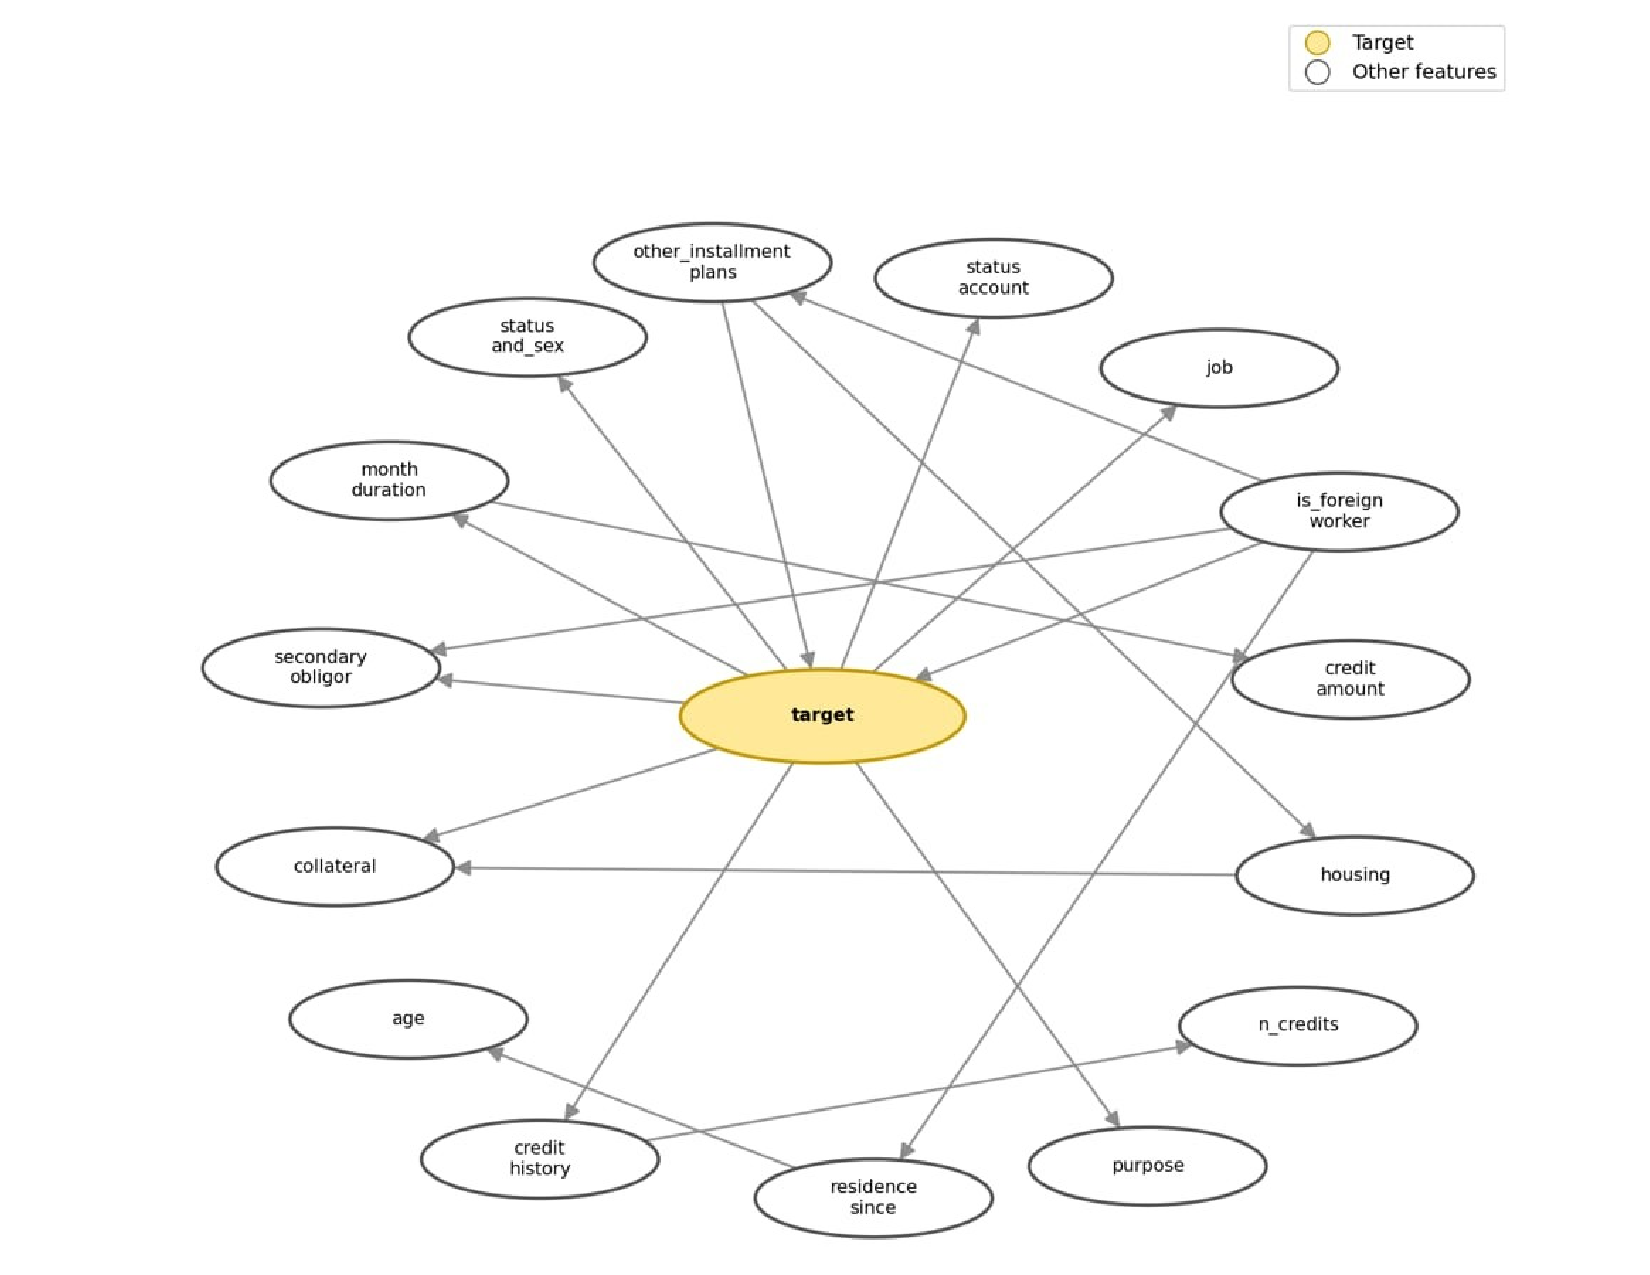
\includegraphics[width=1.1\textwidth,
        height=0.5\textheight,
        trim=2.5cm 0.5cm 2cm 3.5cm,
        clip]{image/network/graph_ger.pdf}
        \caption{Sơ đồ cấu trúc mạng Bayes German Credit dataset}
        \label{fig:net_ger}
    \end{subfigure}

    \caption{Sơ đồ cấu trúc mạng Bayes (Phần 1)}
\end{figure}

\begin{figure}[H]
    \ContinuedFloat % <-- Lệnh quan trọng giúp giữ nguyên số thứ tự Hình (vd: vẫn là Hình 4.5)
    \centering
    
    % --- HÀNG 3: Lending Credit ---
    \begin{subfigure}[b]{1\textwidth}
         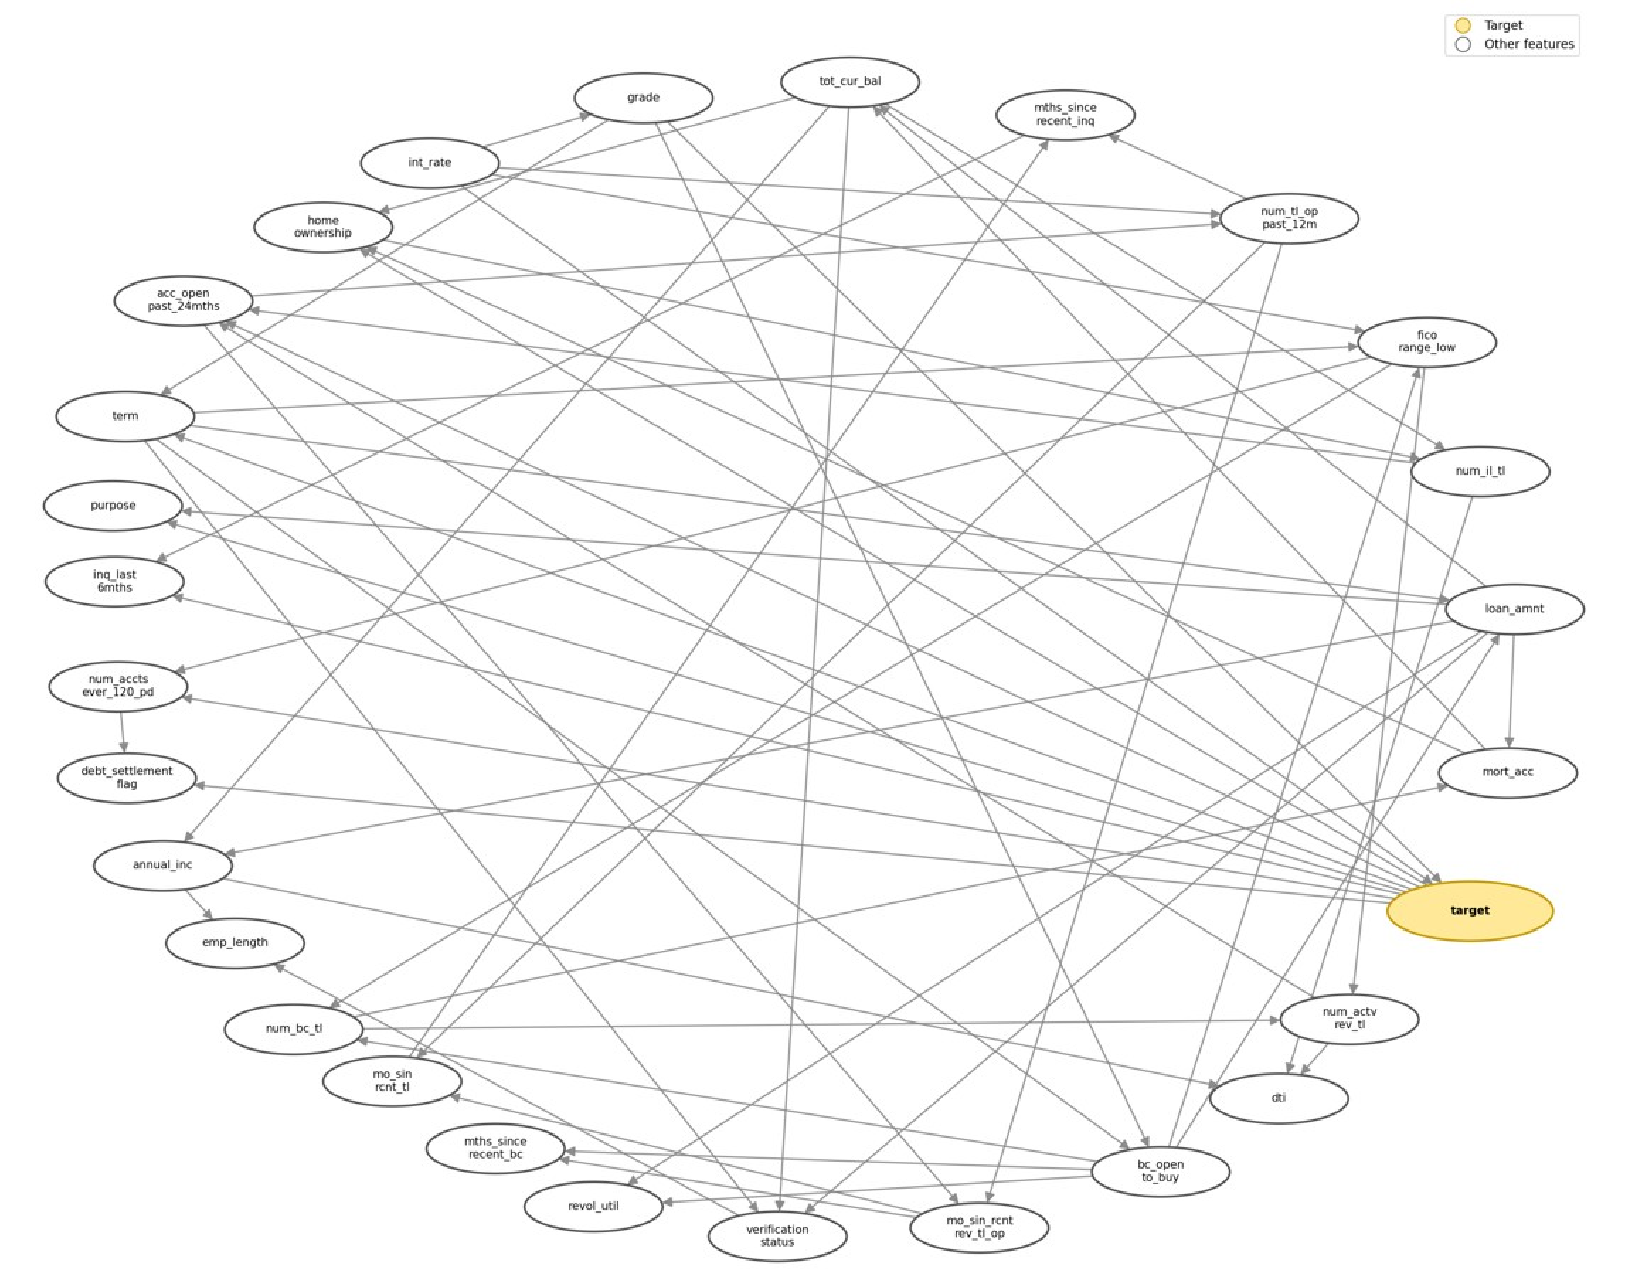
\includegraphics[angle=90,
         width=1.05\textwidth,
        height=1    \textheight,
        trim=0.5cm 0cm 1cm 0.95cm,
        clip]{image/network/graph_lend.pdf}
        \caption{Sơ đồ cấu trúc mạng Bayes Lending Club dataset}
        \label{fig:net_lc}
    \end{subfigure}
    
    \caption{Sơ đồ cấu trúc mạng Bayes (tiếp theo).}
    \label{fig:net}
\end{figure}

\FloatBarrier

Hình \ref{fig:net} cho thấy độ phức tạp cấu trúc đồ thị tỉ lệ thuận với số lượng đặc trưng đầu vào: Lending Club với 27 đặc trưng học được một DAG dày đặc tới 58 cạnh, trong khi Australian Credit chỉ với 8 đặc trưng học được một cấu trúc gọn nhẹ 10 cạnh. Độ ổn định của quá trình tối ưu hóa (đo bằng khoảng dao động điểm BIC giữa 50 lần chạy) cũng khác biệt rõ rệt: ở Australian Credit, biên độ dao động BIC giữa các lần chạy rất hẹp (chỉ khoảng 30 đơn vị quanh giá trị tối ưu), cho thấy không gian tìm kiếm cấu trúc nhỏ và thuật toán Tabu hội tụ rất ổn định và nhất quán giữa các lần khởi tạo ngẫu nhiên khác nhau. Ngược lại, ở Lending Club, biên độ dao động lớn hơn nhiều (hàng nghìn đơn vị BIC), phản ánh không gian cấu trúc rộng và độ nhạy cao với điểm khởi tạo ngẫu nhiên, đây là hệ quả tất yếu của số lượng biến lớn làm không gian DAG khả dĩ tăng theo cấp số nhân (siêu hàm mũ theo số nút).


Trong cả ba cấu trúc học được, biến target có nhiều liên kết trực tiếp (cạnh đến hoặc đi từ target) với các đặc trưng tín dụng cốt lõi, phản ánh đúng trực giác miền (domain knowledge) về rủi ro tín dụng:

\begin{itemize}
    \item Lending Club: target liên kết trực tiếp với int\_rate (lãi suất), grade (xếp hạng tín dụng), debt\_settlement\_flag, num\_accts\_ever\_120\_pd (số tài khoản từng quá hạn 120 ngày), inq\_last\_6mths (số lần truy vấn tín dụng 6 tháng gần nhất), purpose, term, acc\_open\_past\_24mths và home\_ownership.
    
    \item German Credit: target liên kết trực tiếp với status\_account (số dư tài khoản vãng lai), purpose, credit\_history, job, collateral, secondary\_obligor, month\_duration và status\_and\_sex, đồng thời chịu ảnh hưởng trực tiếp từ is\_foreign\_worker và other\_installment\_plans.

    \item Australian Credit: target liên kết trực tiếp và duy nhất với ba biến CreditHistory, Employed và Income, phản ánh cấu trúc nhân quả rất gọn của bộ dữ liệu này.
\end{itemize}

Sự nhất quán giữa cấu trúc đồ thị học được bằng thuật toán dữ liệu thuần túy (data-driven) và kiến thức chuyên gia tín dụng truyền thống (ví dụ lịch sử tín dụng, lãi suất, thu nhập là các yếu tố quyết định) là một chỉ dấu định tính quan trọng cho thấy mô hình BN không chỉ có khả năng dự đoán mà còn có khả năng diễn giải nhân quả hợp lý.

Bên cạnh cấu trúc đồ thị thuần túy, Hình \ref{fig:marginal_australian}, \ref{fig:marginal_german} và \ref{fig:marginal_lendingclub}  trình bày toàn cảnh mạng Bayes của ba bộ dữ liệu kèm theo phân phối biên (marginal distribution) tiên nghiệm của từng node, tức phân phối xác suất của mỗi biến khi chưa có bất kỳ bằng chứng nào được đưa vào, bao gồm cả biến \texttt{target} ở mức 50\%/50\% do đã qua bước cân bằng dữ liệu SMOTE-NC tại $S_{\text{Pro}}$. Cách trực quan hóa này cho phép quan sát đồng thời cả cấu trúc phụ thuộc lẫn hình dạng phân phối của từng biến ngay trên cùng một sơ đồ, thay vì phải tra cứu riêng lẻ từng bảng CPT.

Trên Australian Credit (Hình \ref{fig:marginal_australian}), phân phối biên cho thấy phần lớn khách hàng thuộc nhóm quốc tịch/cư trú state 2 (90.8\%), trong khi \texttt{CreditHistory} và \texttt{Employed} phân bố tương đối cân bằng giữa hai trạng thái (42.9\%/57.1\% và 53.9\%/46.1\%), phản ánh đúng tính chất một bộ dữ liệu đã được xử lý cân bằng nhãn nhưng các đặc trưng đầu vào vẫn giữ nguyên phân phối tự nhiên.

Trên German Credit (Hình \ref{fig:marginal_german}), đáng chú ý là \texttt{is\_foreign\_worker} lệch mạnh về state 1 (83.0\%) và \texttt{secondary\_obligor} lệch mạnh về state 2 "guarantor" (73.2\%), cho thấy đây là hai đặc trưng có phân phối tự nhiên mất cân bằng rõ rệt trong tổng thể dữ liệu, một yếu tố cần lưu ý khi diễn giải các kết quả suy luận tiến/lùi liên quan đến hai biến này ở Mục \ref{sec:4.4.1} và \ref{sec:4.4.2}, vì các trạng thái thiểu số (\texttt{is\_foreign\_worker}=0, \texttt{secondary\_obligor}$\in\{0,1\}$) vốn dĩ đã có ít quan sát hỗ trợ ngay từ đầu.

Trên Lending Club (Hình \ref{fig:marginal_lendingclub}), \texttt{debt\_settlement\_flag} lệch cực mạnh về state 0 (98\%), chỉ 2\% khách hàng từng tham gia chương trình tái cơ cấu nợ, đây chính là gốc rễ của hiện tượng dữ liệu thưa khi biến này liên tục cho ra các giá trị xác suất cực trị ($\delta=0.5$, hoặc xác suất hậu nghiệm bão hòa 100\%). Tương tự, \texttt{num\_accts\_ever\_120\_pd} cũng lệch mạnh về state 0 (73.1\%). Việc quan sát trước phân phối biên như vậy giúp lý giải có cơ sở cho các kết quả bất thường xuất hiện xuyên suốt phần thực nghiệm diễn giải mô hình ở các mục sau, thay vì phải suy đoán ngược lại từ kết quả.

\vspace{1em}
\begin{table}[ht]
\centering
\caption{Tổng hợp chỉ số đánh giá mô hình mạng Bayes trên tập huấn luyện và tập kiểm tra}
\label{tab:bn_train_test}

\renewcommand{\arraystretch}{1.3}

\begin{tabular}{|
p{2.5cm}|
>{\centering\arraybackslash}p{1.5cm}|
>{\centering\arraybackslash}p{1.5cm}|
>{\centering\arraybackslash}p{1.5cm}|
>{\centering\arraybackslash}p{1.5cm}|
>{\centering\arraybackslash}p{1.5cm}|
>{\centering\arraybackslash}p{1.5cm}|}

\hline
\rowcolor{gray!20}

\makecell{\centering \textcolor{black}{\textbf{Chỉ số}}} &
\multicolumn{2}{c|}{\textcolor{black}{\textbf{Lending Club}}} &
\multicolumn{2}{c|}{\textcolor{black}{\textbf{German Credit}}} &
\multicolumn{2}{c|}{\textcolor{black}{\textbf{Australian Credit}}} \\

\cline{2-7}

\rowcolor{gray!20}
&
\multicolumn{1}{>{\columncolor{gray!20}}c|}{\textcolor{black}{\textbf{Train}}} &
\multicolumn{1}{>{\columncolor{gray!20}}c|}{\textcolor{black}{\textbf{Test}}} &
\multicolumn{1}{>{\columncolor{gray!20}}c|}{\textcolor{black}{\textbf{Train}}} &
\multicolumn{1}{>{\columncolor{gray!20}}c|}{\textcolor{black}{\textbf{Test}}} &
\multicolumn{1}{>{\columncolor{gray!20}}c|}{\textcolor{black}{\textbf{Train}}} &
\multicolumn{1}{>{\columncolor{gray!20}}c|}{\textcolor{black}{\textbf{Test}}} \\

\hline

Accuracy
& 0.7085 & 0.6808
& 0.7811 & 0.7300
& 0.8641 & 0.8406 \\

\hline

Precision
& 0.7269 & 0.4610
& 0.8386 & 0.6047
& 0.9247 & 0.9211 \\

\hline

Recall 
& 0.6679 & 0.4878
& 0.6962 & 0.4127
& 0.7926 & 0.8140 \\

\hline

Specificity
& 0.7490 & 0.7615
& 0.8660 & 0.8759
& 0.9355 & 0.8846 \\

\hline

F1-Score
& 0.7034 & 0.4740
& 0.7608 & 0.4906
& 0.8536 & 0.8642 \\


\hline

ROC-AUC
& 0.7944 & 0.6910
& 0.8686 & 0.7667
& 0.9278 & 0.9220 \\

\hline

PR-AUC
& 0.8238 & 0.5224
& 0.8886 & 0.5421
& 0.9070 & 0.9371 \\

\hline

\end{tabular}
\end{table}
\FloatBarrier

\vspace{1em}
Kết quả ở Bảng \ref{tab:bn_train_test} cho thấy một xu hướng rõ rệt: hiệu năng dự đoán của mô hình BN tăng dần theo chiều Lending Club $\rightarrow$ German Credit $\rightarrow$ Australian Credit, với ROC-AUC lần lượt là 0.6910, 0.7667 và 0.9220. Điều này có thể được lý giải từ ba góc độ. Mức độ nhiễu nội tại của dữ liệu, Lending Club là dữ liệu cho vay tiêu dùng thực tế quy mô lớn với hành vi vỡ nợ phụ thuộc vào nhiều yếu tố ngẫu nhiên ngoài hồ sơ tín dụng (thất nghiệp đột xuất, biến động kinh tế vĩ mô...), trong khi German và Australian Credit là dữ liệu chuẩn hóa cao của UCI, vốn đã qua xử lý và có quan hệ đặc trưng, nhãn rõ ràng hơn. Độ phức tạp số chiều, số đặc trưng càng nhiều (27 so với 8) thì không gian CPT của mạng Bayes càng phức tạp, dễ dẫn đến hiện tượng dữ liệu thưa (data sparsity) trong các bảng xác suất có điều kiện và làm giảm độ chính xác ước lượng tham số. Đối với Australian Credit, do prevalence của nhãn default cao ($\approx 58 \%$), bài toán phân loại có phần dễ hơn về mặt thống kê khi không phải đối mặt với độ mất cân bằng cực đoan trên tập test.

Trên bộ Lending Club, AUC trên tập train đạt 0.7944 trong khi AUC trên tập test chỉ đạt 0.6910, mức chênh lệch khá lớn ($\approx 0.1034$), cho thấy mô hình có dấu hiệu overfitting nhẹ đến trung bình đối với cấu trúc đồ thị 58 cạnh học được từ 27 biến. Đây là hệ quả hợp lý của việc mạng Bayes rời rạc với CPT có số tổ hợp trạng thái lớn (do nhiều biến và nhiều cạnh) dễ khớp quá mức với phân phối thực nghiệm của tập huấn luyện. Đối với Australian Credit có cấu trúc gọn hơn, ít cạnh hơn, khoảng cách train–test được kỳ vọng hẹp hơn đáng kể do số bậc tự do (degrees of freedom) của mô hình thấp hơn nhiều so với cỡ mẫu.

\begin{figure}[h]
\centering
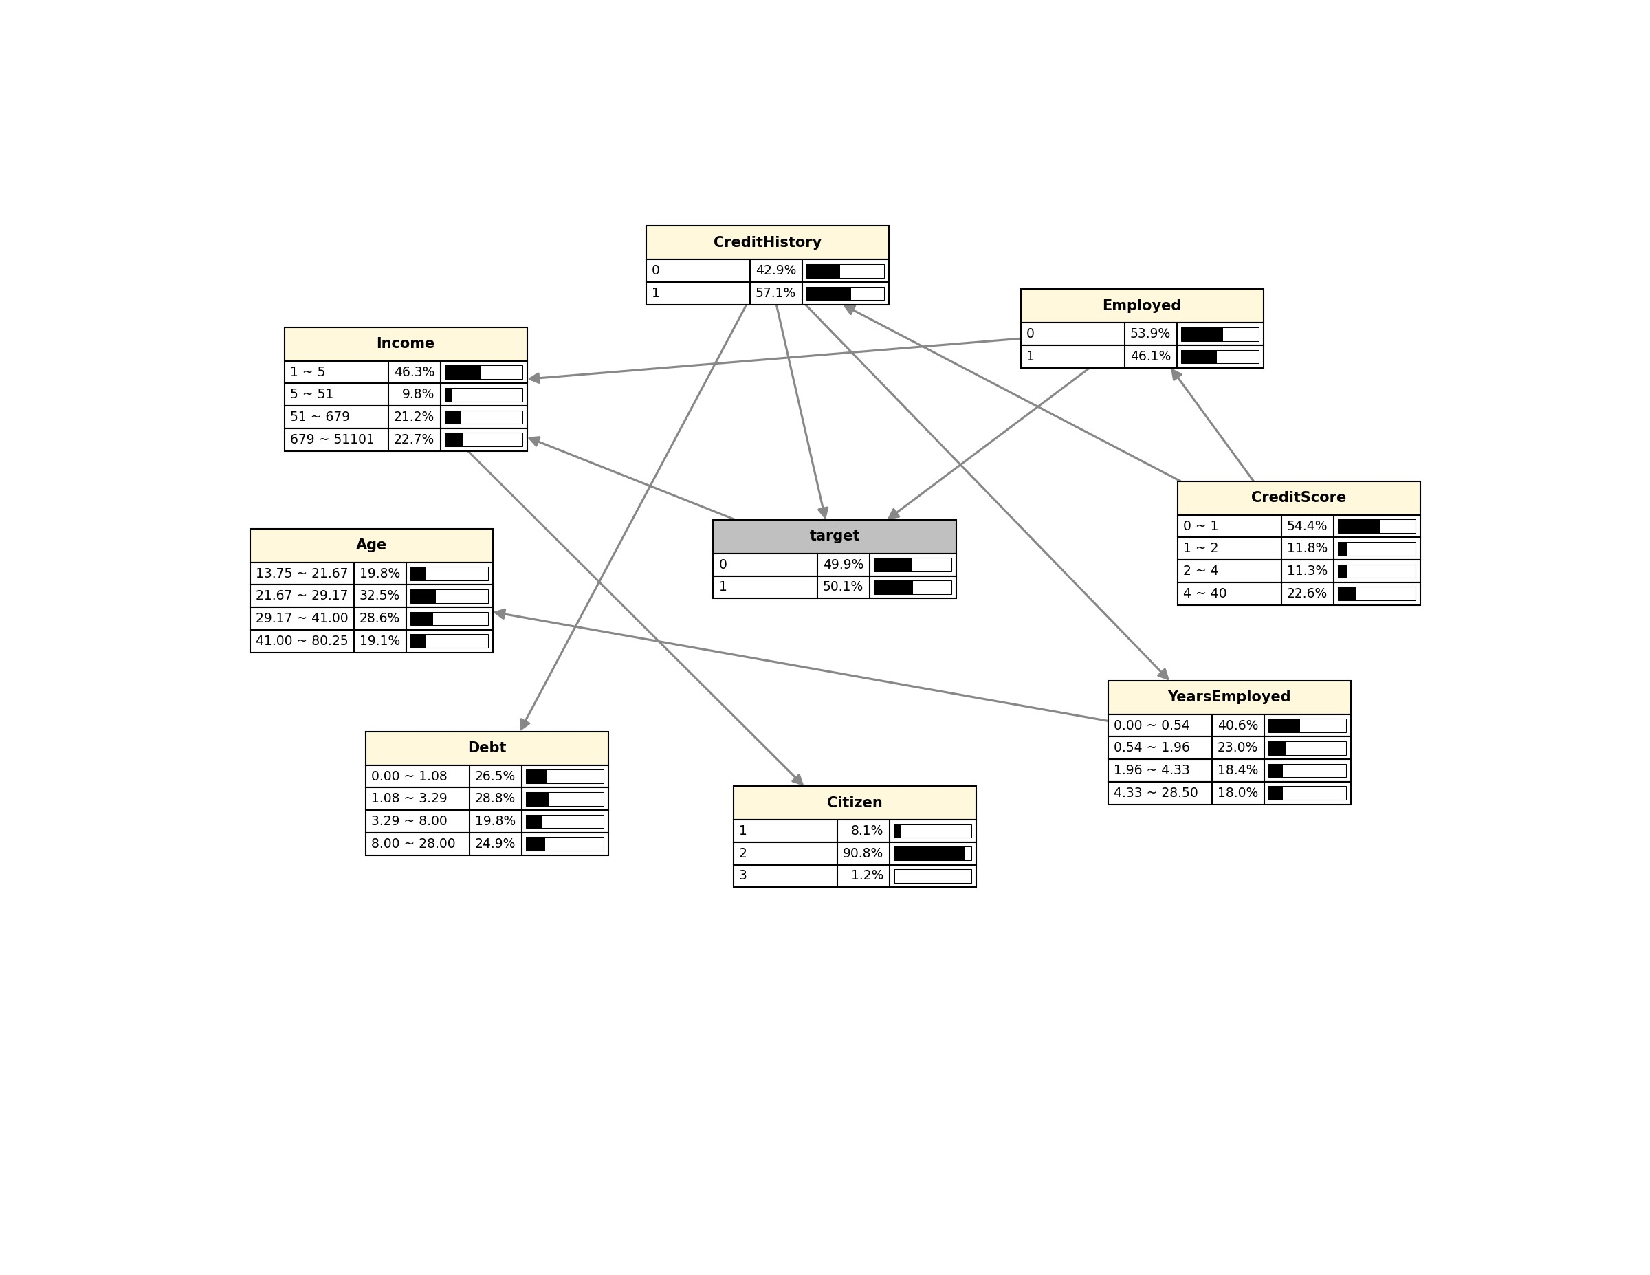
\includegraphics[
    width=1.05\textwidth,
    height=0.6\textheight,
    trim=3cm 5cm 3cm 3cm,
    clip
]{image/au_back.pdf}
\caption{Phân phối xác suất của toàn mạng --- Australian Credit}
\label{fig:marginal_australian}
\end{figure}

\begin{figure}[h]
\centering
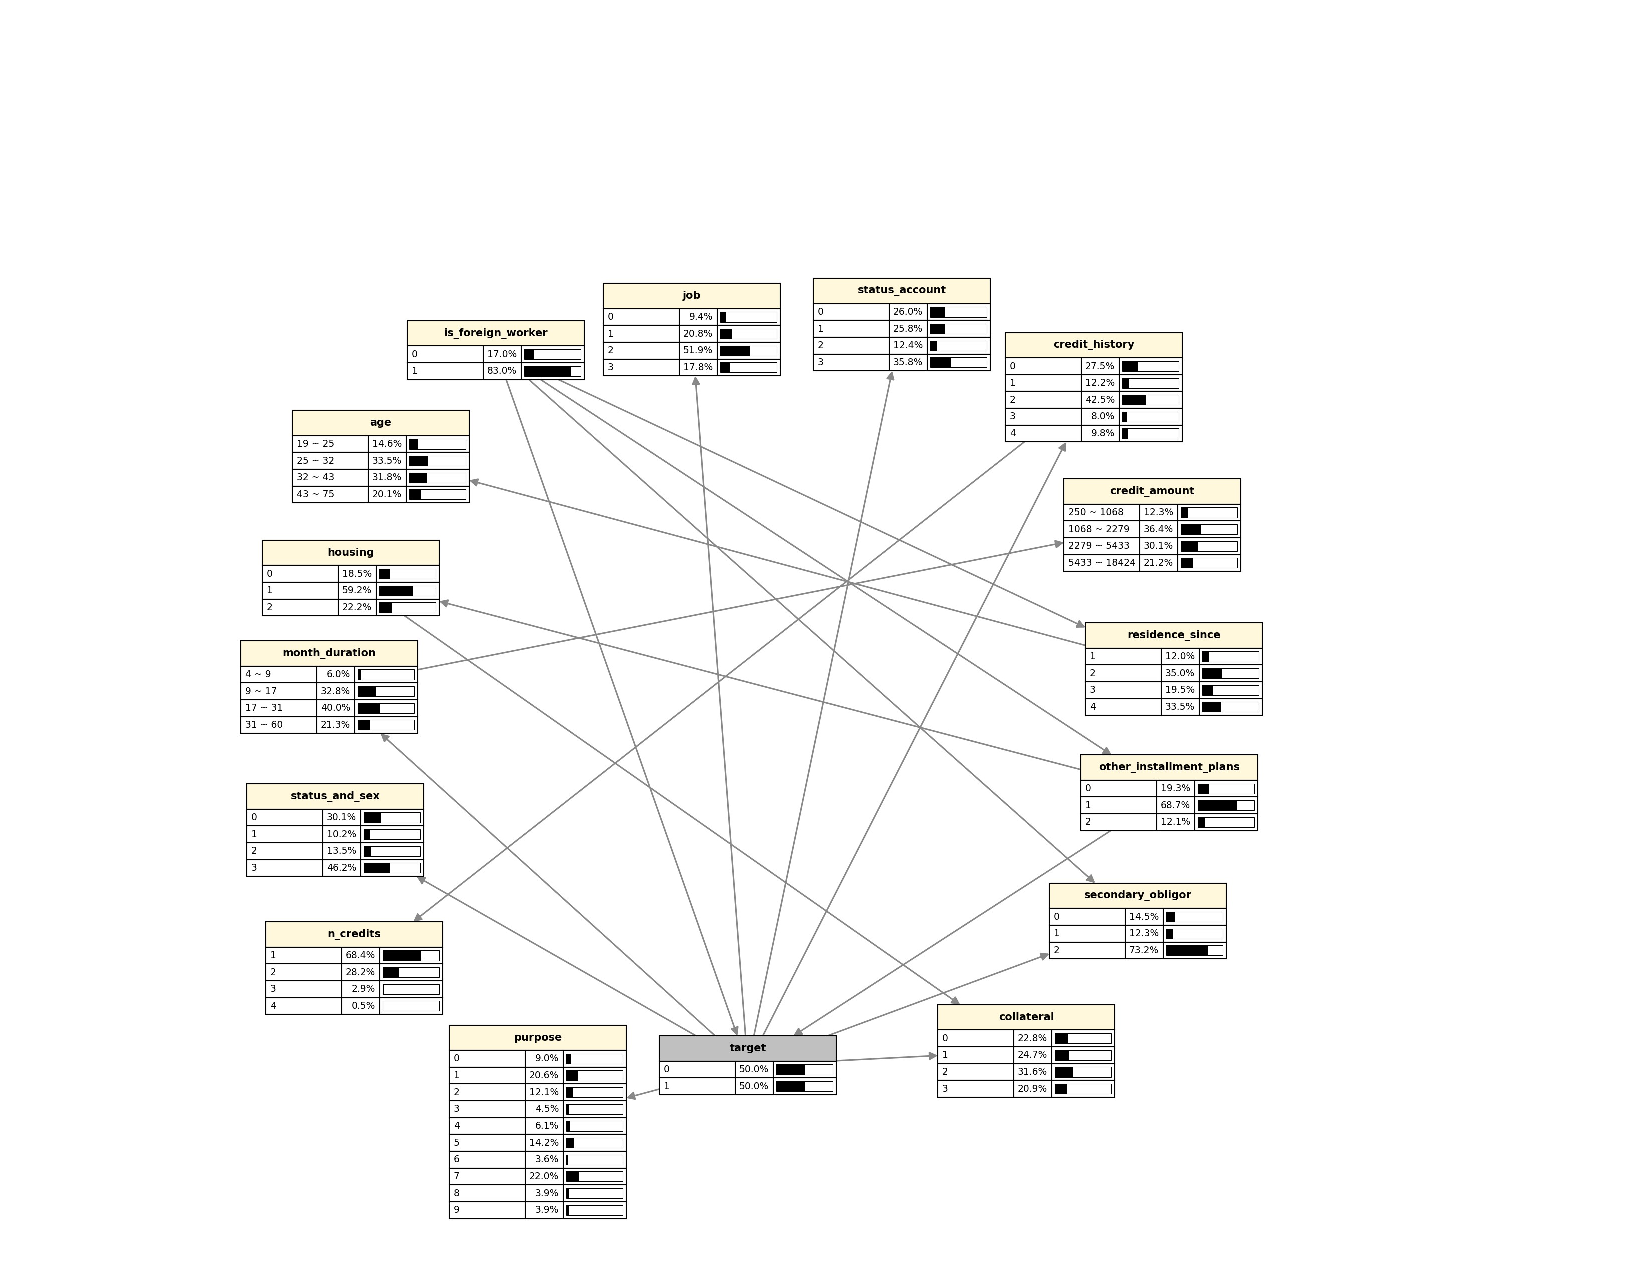
\includegraphics[
    width=1.2\textwidth,
    height=0.8\textheight,
    trim=3cm 0.5cm 3cm 3cm,
    clip
]{image/ger_back.pdf}
\caption{Phân phối xác suất của toàn mạng --- German Credit}
\label{fig:marginal_german}
\end{figure}

\begin{figure}[h]
\centering
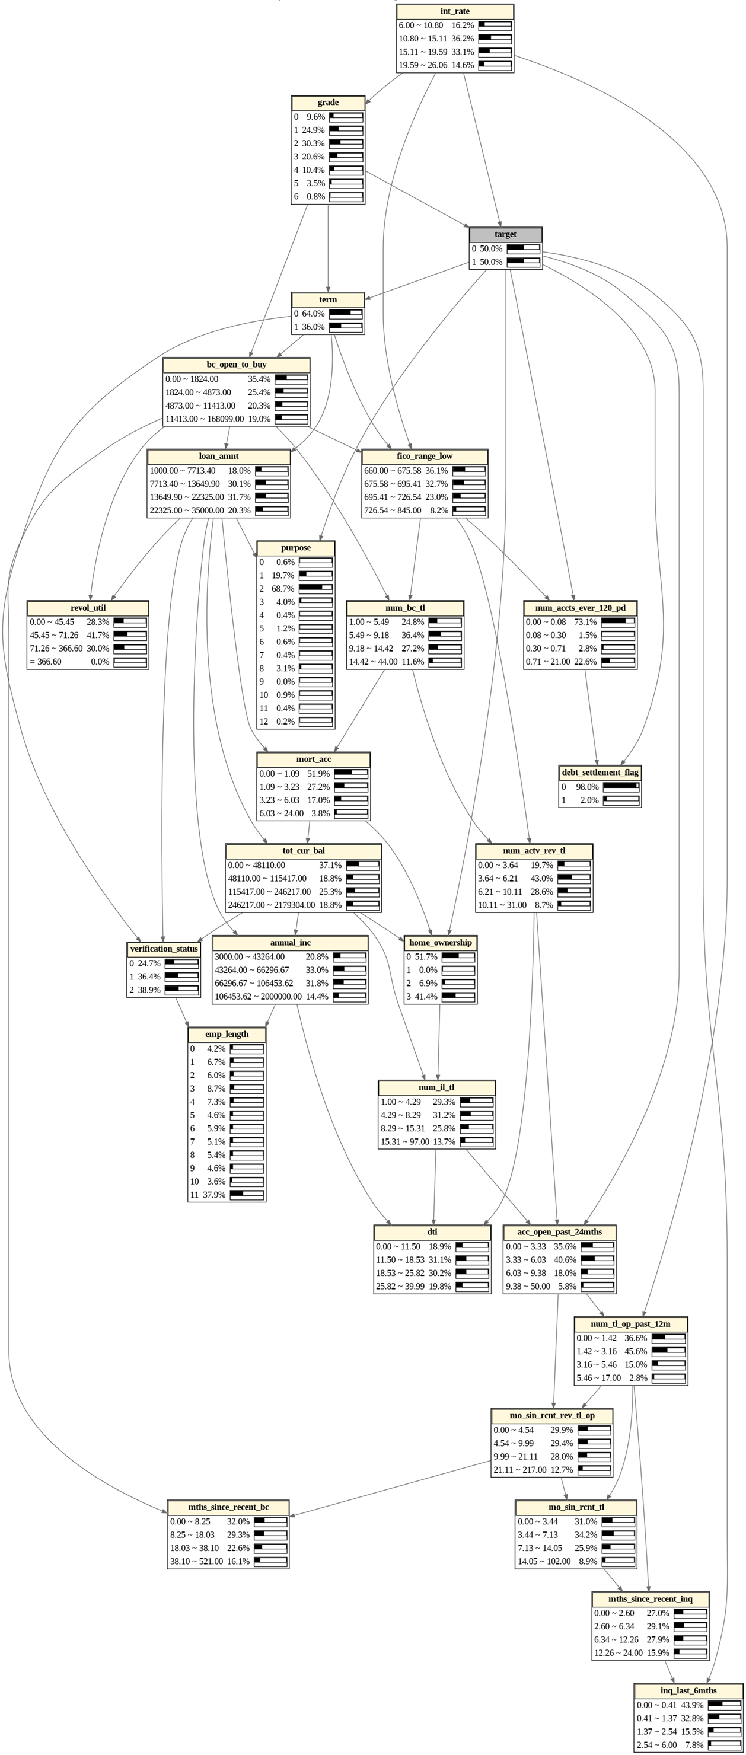
\includegraphics[width=1.1\textwidth,height=\textheight]{image/lend_back.pdf}
\caption{Phân phối xác suất của toàn mạng --- Lending Club}
\label{fig:marginal_lendingclub}
\end{figure}

\FloatBarrier
\subsubsection{Phân tích đường cong ROC, ngưỡng tối ưu và Decision Curve Analysis trên tập Validation}

\noindent
\textbf{\textit{Australian Credit}}

\begin{figure}[H]
    \centering
    \begin{subfigure}[b]{0.7\textwidth} % Giảm nhẹ xuống 0.8 để 2 hình chắc chắn vừa 1 trang
        \centering
        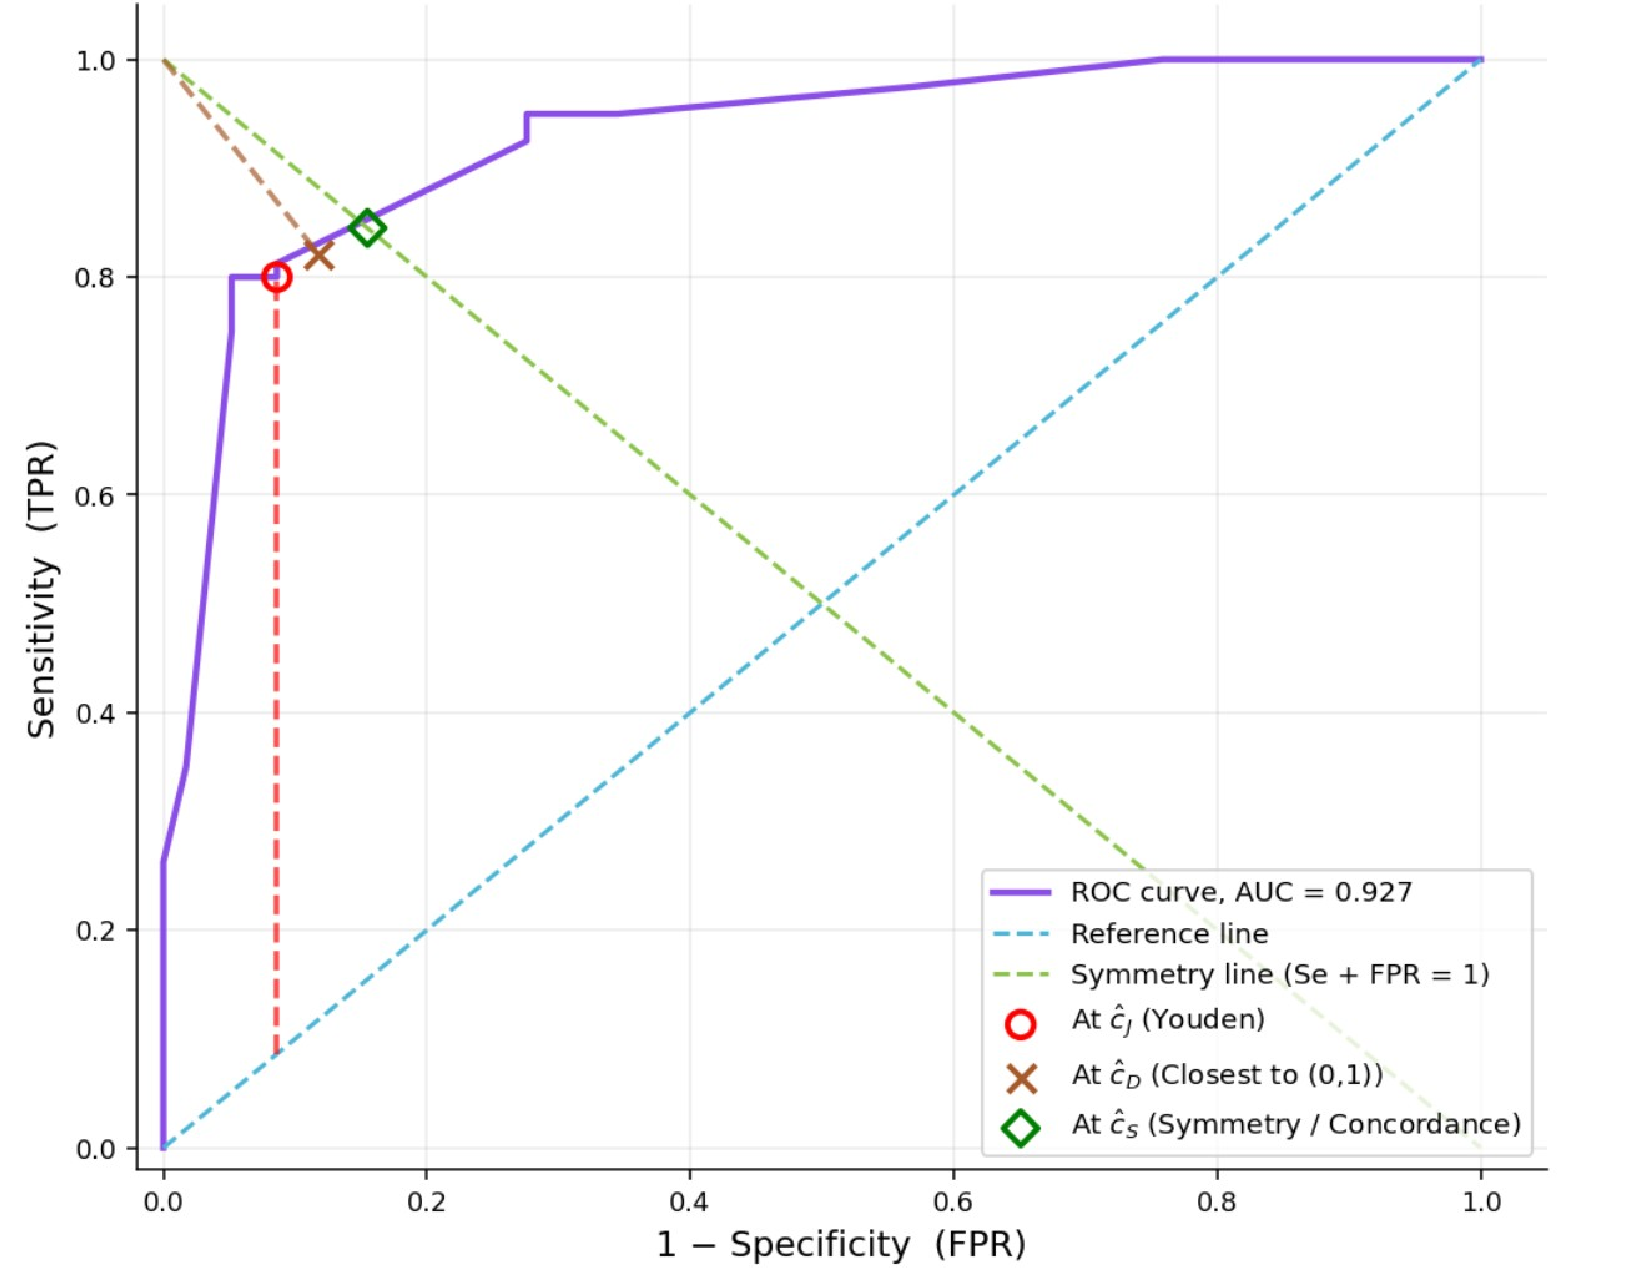
\includegraphics[width=\textwidth]{image/roc_dca/roc_au.pdf}
    \end{subfigure}
    \caption{Đồ thị ba ngưỡng quyết định tối ưu theo ROC --- Australian Credit}
    \label{fig:roc_au}
\end{figure}

\begin{figure}[H]
    \centering
    \begin{subfigure}[b]{0.7\textwidth}
        \centering
        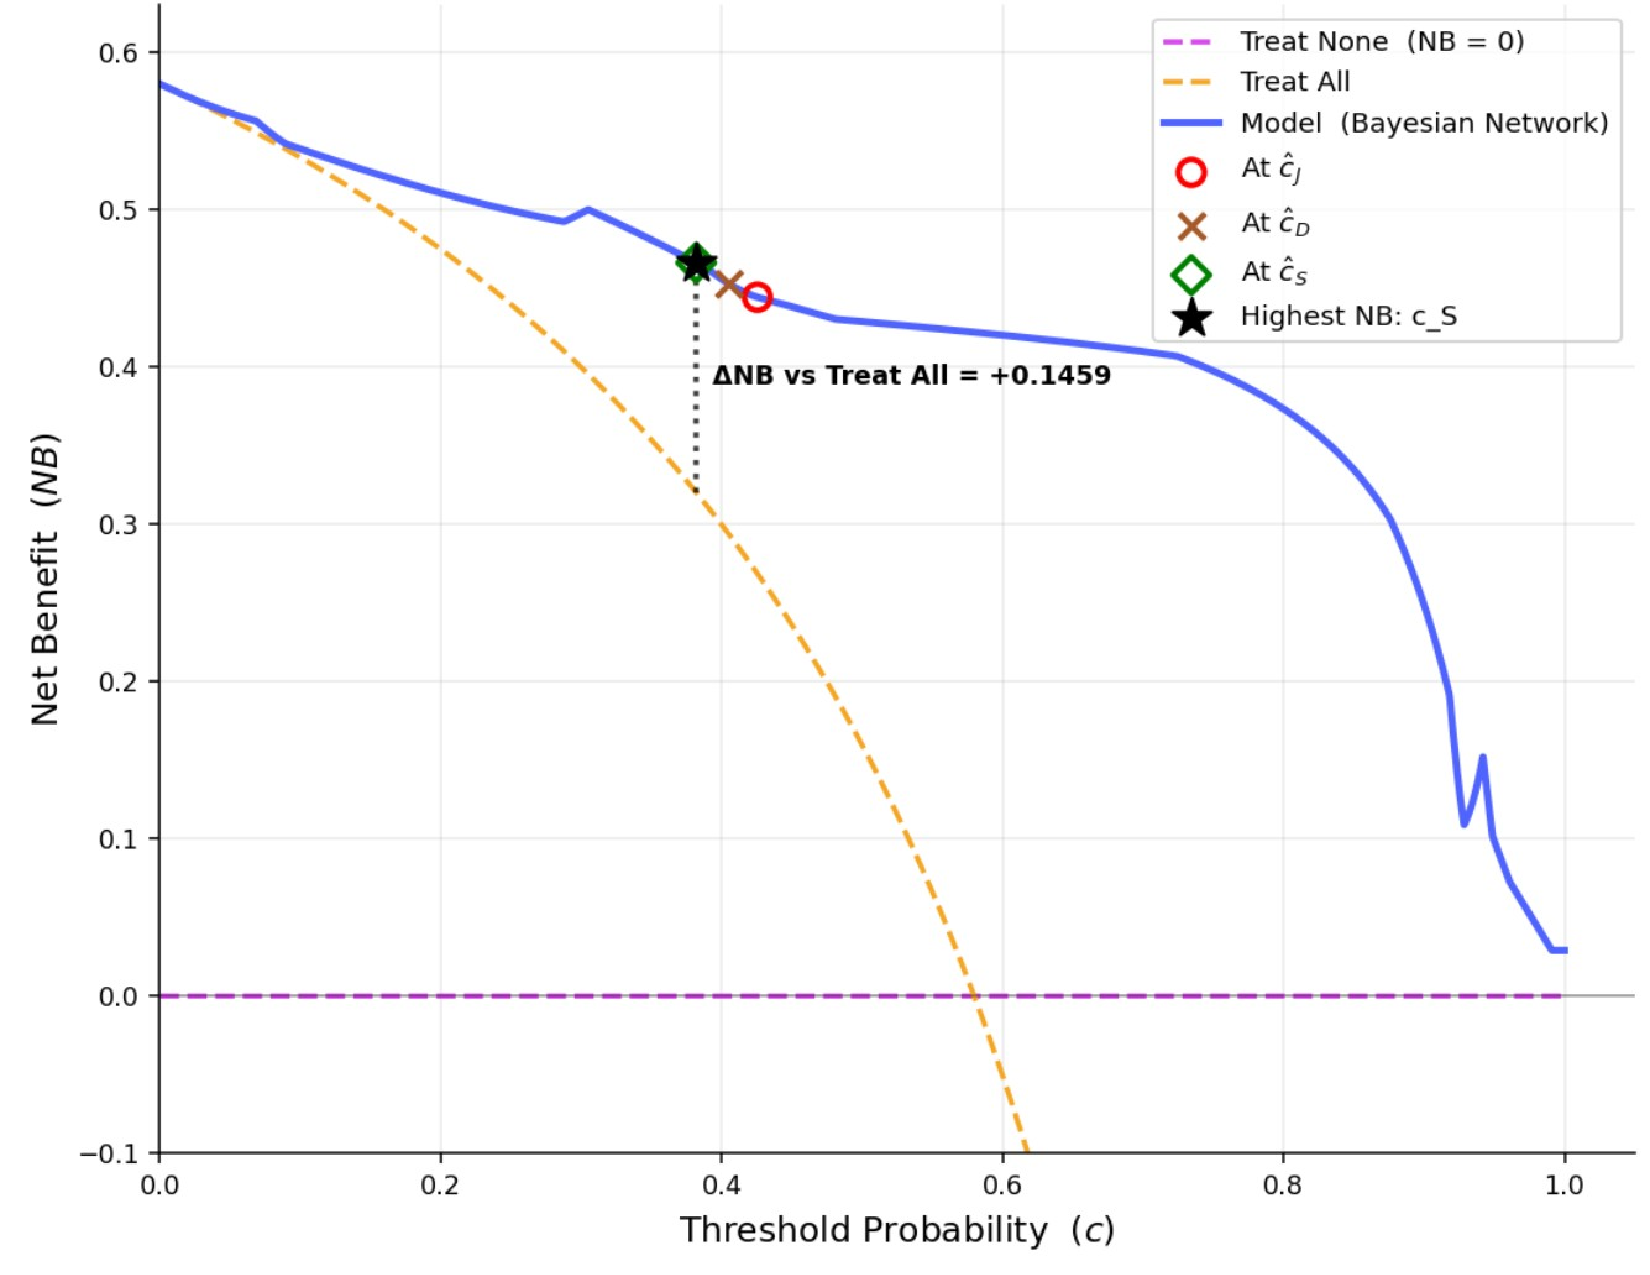
\includegraphics[width=\textwidth]{image/roc_dca/dca_au.pdf}
    \end{subfigure}
    \caption{Đồ thị ba ngưỡng quyết định tối ưu trên DCA --- Australian Credit}
    \label{fig:dca_au}
\end{figure}

\begin{table}[H]
\centering
\caption{Ba ngưỡng quyết định tối ưu theo ROC -- Australian Credit (tập validation)}
\label{tab:roc_threshold}

\renewcommand{\arraystretch}{1.3}

\begin{tabular}{|p{4cm}|c|c|c|c|c|}
\hline
\rowcolor{gray!20}
\centering\textbf{Tiêu chí ngưỡng} &
\centering\textbf{Ngưỡng (c)} &
\centering\textbf{Sensitivity} &
\centering\textbf{Specificity} &
\centering\textbf{Accuracy} &
\centering\arraybackslash\textbf{F1-Score} \\
\hline

Youden Index &
0.4254 &
0.8125 &
0.9138 &
0.8551 &
0.8667 \\
\hline

Closest to (0,1) &
0.4052 &
0.8125 &
0.9138 &
0.8551 &
0.8667 \\
\hline

Symmetry Point &
0.3818 &
0.9250 &
0.7241 &
0.8406 &
0.8706 \\
\hline

\end{tabular}
\end{table}

Kết quả DCA dựa vào Hình \ref{fig:roc_au}, \ref{fig:dca_au} và Bảng \ref{tab:roc_threshold}: với prevalence = 0.5797, Ngưỡng Symmetry Point ($c_S = 0.3818$) cho Net Benefit cao nhất trong ba ngưỡng (NB = 0.4661), vượt Treat All 0.1459 điểm.

\vspace{1em}
\noindent
\textbf{\textit{German Credit}}

Kết quả DCA dựa vào Hình \ref{fig:roc_ger}, \ref{fig:dca_ger} và Bảng \ref{tab:roc_threshold_german}: prevalence (tỉ lệ default) trên tập validation = 0.2750. Trong ba ngưỡng ROC tối ưu, ngưỡng Closest-to (0,1) ($c_D = 0.1895$) cho Net Benefit cao nhất (NB = 0.1474), vượt Treat All 0.0419 điểm Net Benefit.

\begin{figure}[H]
    \centering
    \begin{subfigure}[b]{0.85\textwidth} % Giảm nhẹ xuống 0.8 để 2 hình chắc chắn vừa 1 trang
        \centering
        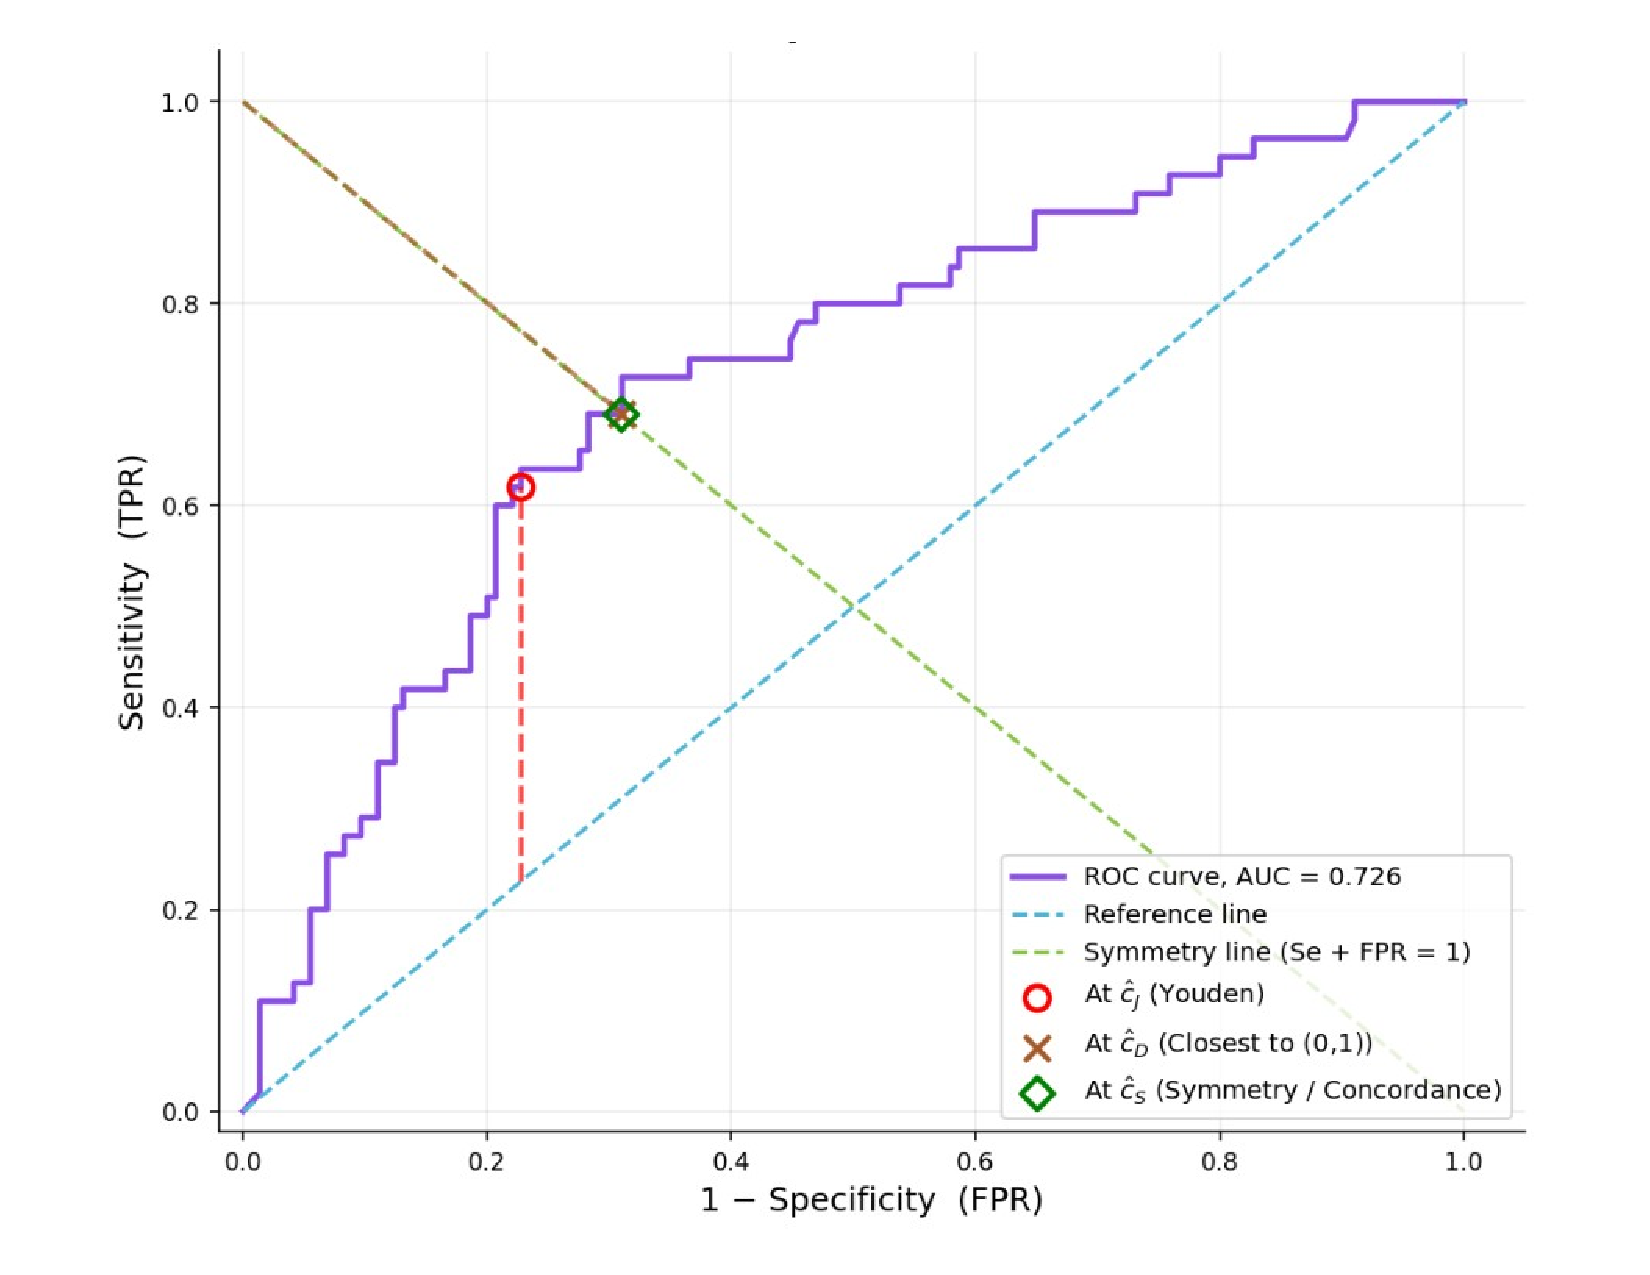
\includegraphics[width=\textwidth]{image/roc_dca/roc_ger.pdf}
    \end{subfigure}
    \caption{Đồ thị ba ngưỡng quyết định tối ưu theo ROC --- German Credit}
    \label{fig:roc_ger}
\end{figure}

\begin{figure}[H]
    \centering
    \begin{subfigure}[b]{0.85\textwidth}
        \centering
        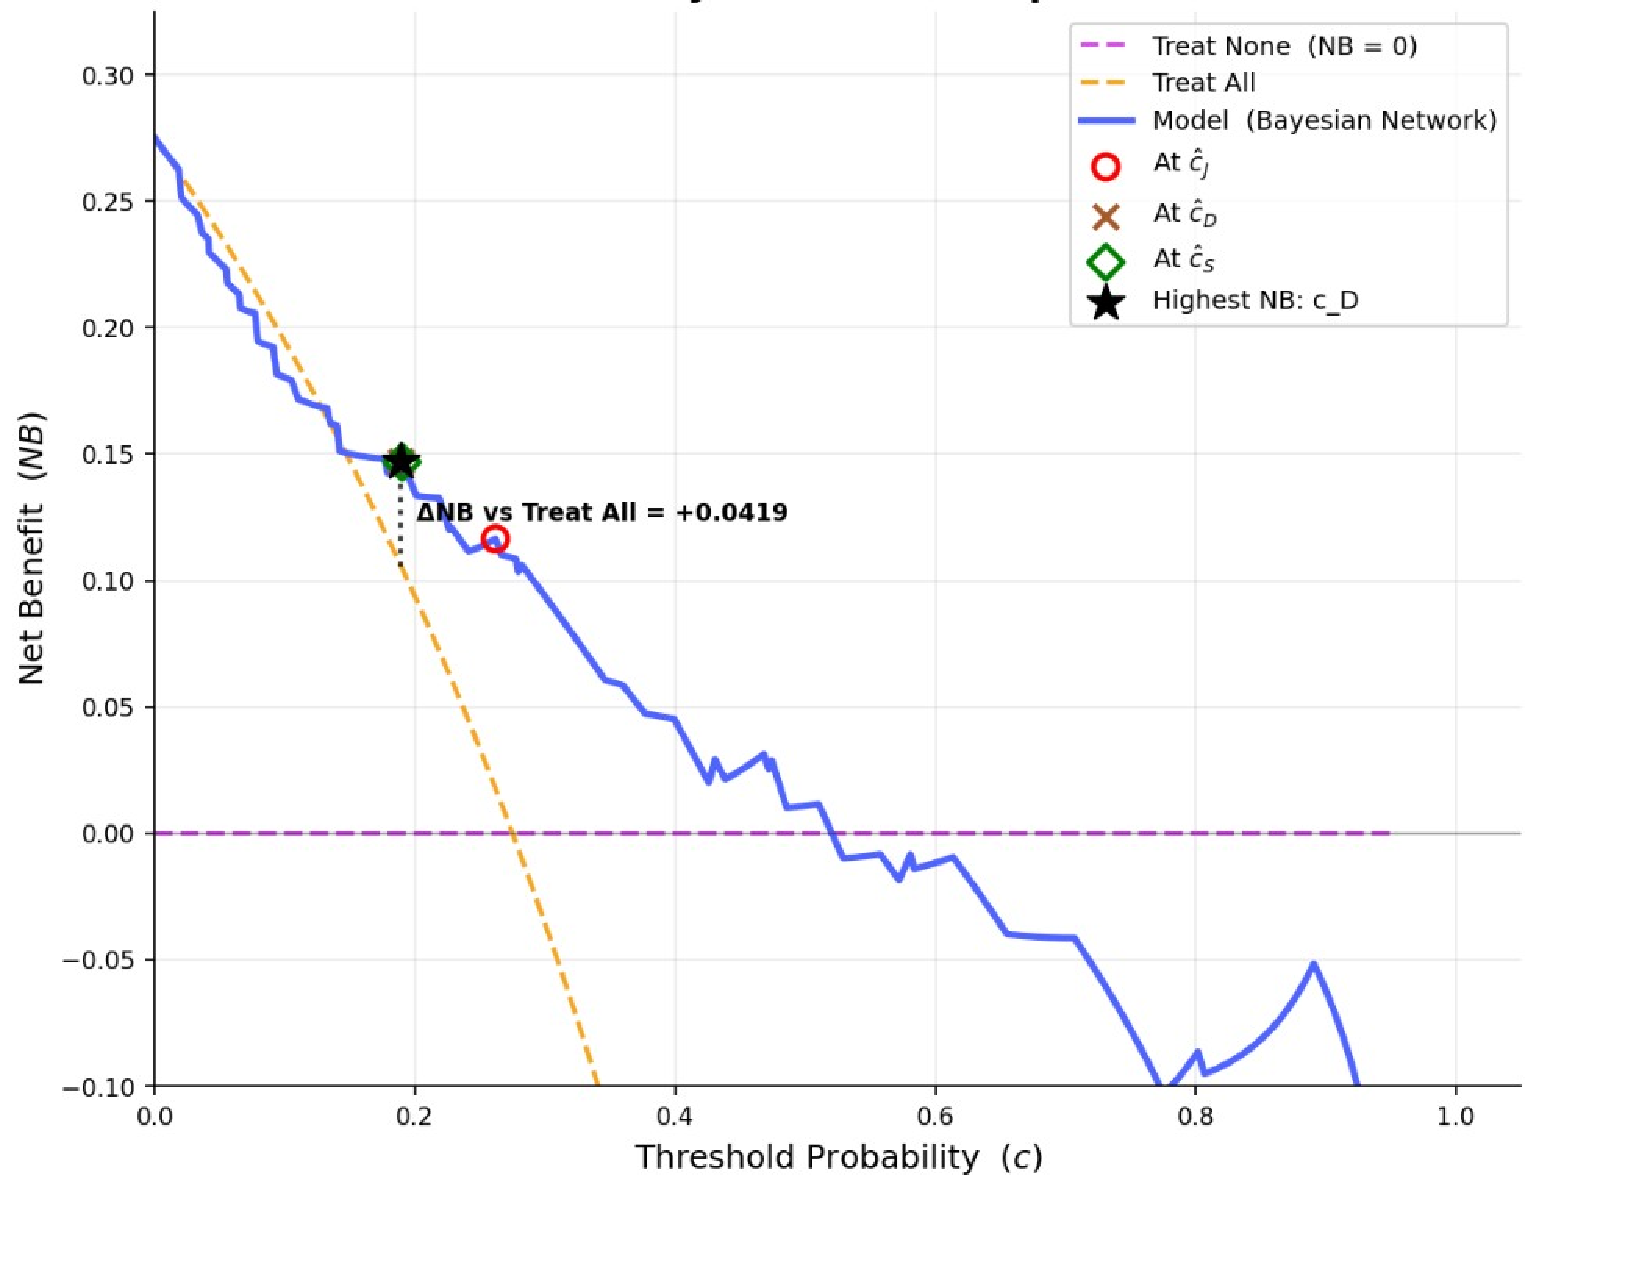
\includegraphics[width=\textwidth]{image/roc_dca/dca_ger.pdf}
    \end{subfigure}
    \caption{Đồ thị ba ngưỡng quyết định tối ưu trên DCA --- German Credit}
    \label{fig:dca_ger}
\end{figure}

\begin{table}[H]
\centering
\caption{Ba ngưỡng quyết định tối ưu theo ROC -- German Credit (tập validation)}
\label{tab:roc_threshold_german}

\renewcommand{\arraystretch}{1.3}

\begin{tabular}{|p{4cm}|c|c|c|c|c|}
\hline
\rowcolor{gray!20}
\centering\textbf{Tiêu chí ngưỡng} &
\centering\textbf{Ngưỡng (c)} &
\centering\textbf{Sensitivity} &
\centering\textbf{Specificity} &
\centering\textbf{Accuracy} &
\centering\arraybackslash\textbf{F1-Score} \\
\hline

Youden Index
& 0.2619
& 0.6364
& 0.7724
& 0.7350
& 0.5691 \\
\hline

Closest to (0,1)
& 0.1895
& 0.7091
& 0.6897
& 0.6950
& 0.5612 \\
\hline

Symmetry Point
& 0.1901
& 0.7091
& 0.6897
& 0.6950
& 0.5612 \\
\hline

\end{tabular}
\end{table}

\vspace{1em}
\noindent
\textbf{\textit{Lending Club}}

Kết quả DCA Hình \ref{fig:roc_lend}, \ref{fig:dca_lend} và Bảng \ref{tab:roc_threshold_lending}: prevalence = 0.3017. Đáng chú ý, cả ba ngưỡng đều có Net Benefit của Treat All âm, nên baseline so sánh là Treat None (NB = 0); ngưỡng Youden ($c_J = 0.3431$) cho Net Benefit dương cao nhất trong ba ngưỡng (NB = 0.0561) nhưng ở mức thấp hơn đáng kể so với hai bộ dữ liệu còn lại, cho thấy lợi ích thực tiễn của mô hình BN trên Lending Club hạn chế hơn.

\begin{figure}[H]
    \centering
    \begin{subfigure}[b]{0.85\textwidth} % Giảm nhẹ xuống 0.8 để 2 hình chắc chắn vừa 1 trang
        \centering
        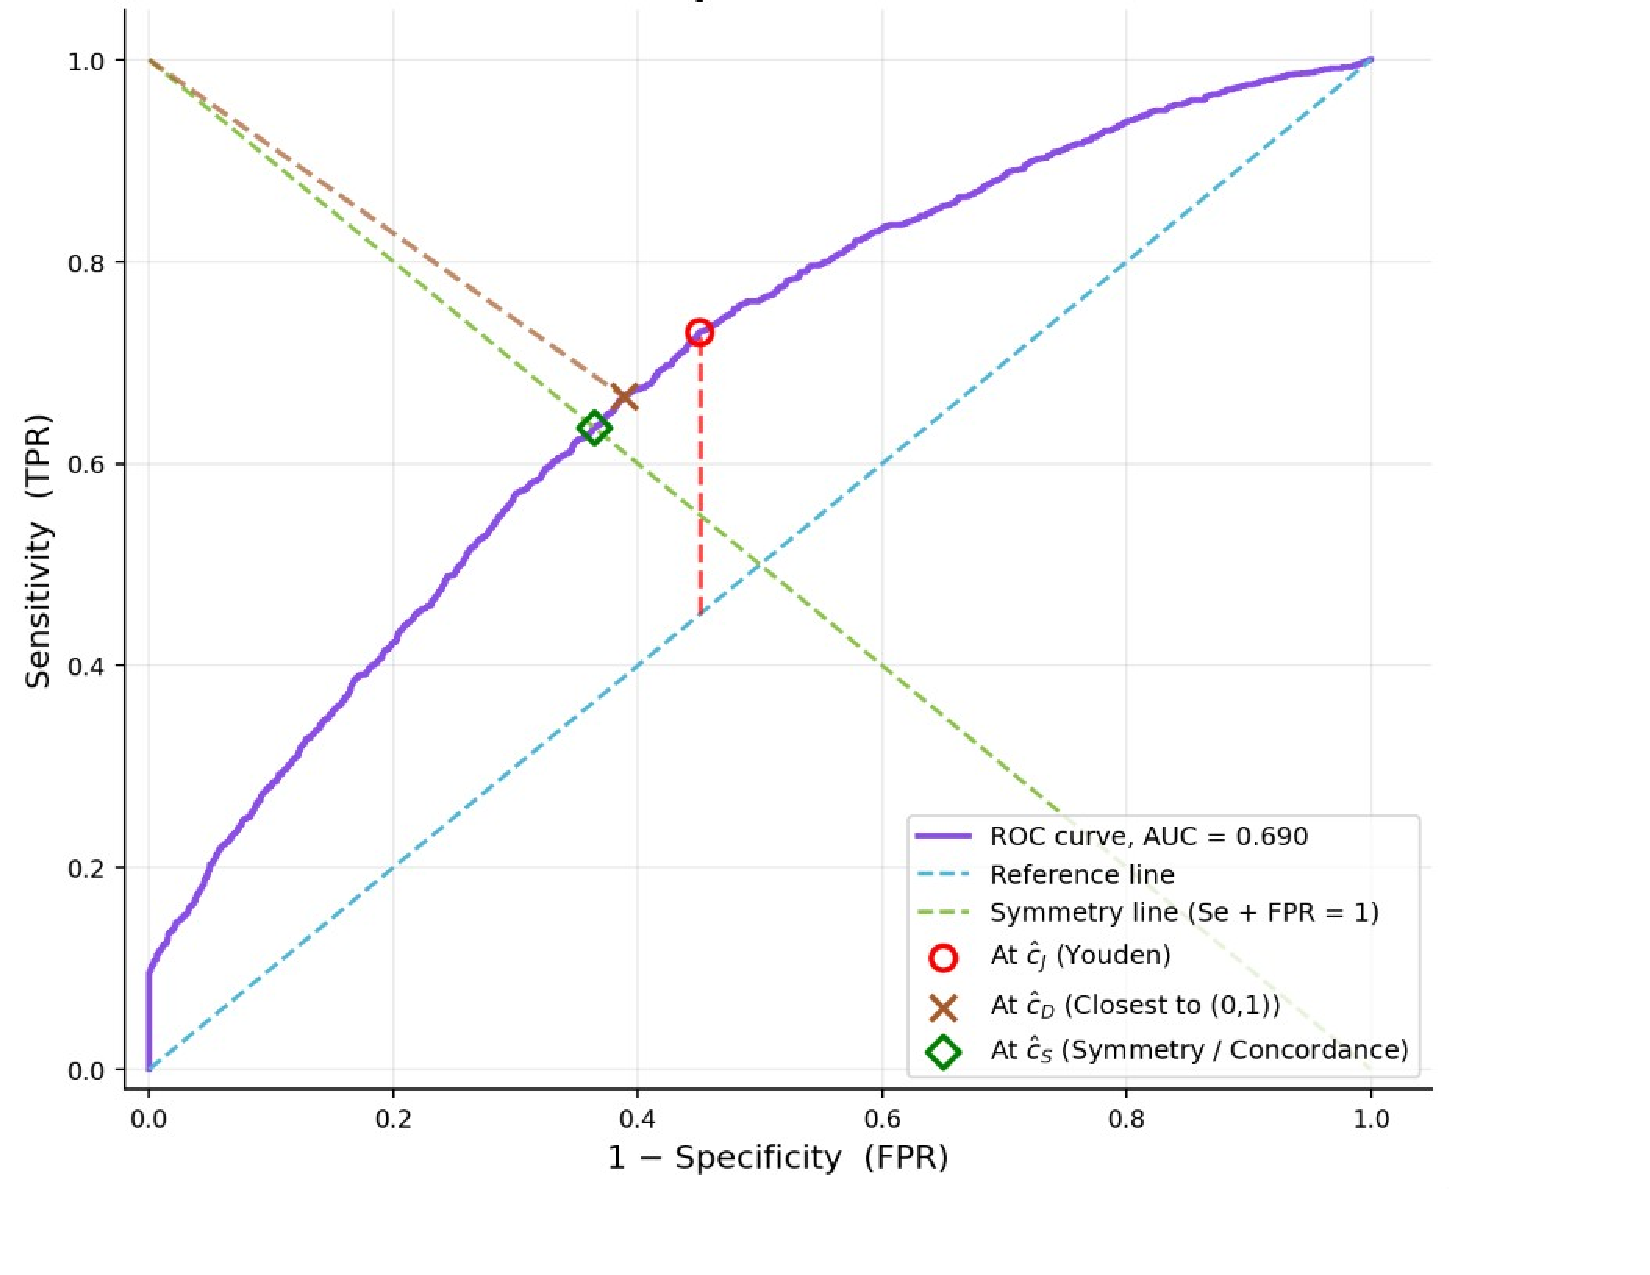
\includegraphics[width=\textwidth]{image/roc_dca/roc_lend.pdf}
    \end{subfigure}
    \caption{Đồ thị ba ngưỡng quyết định tối ưu theo ROC --- Lending Club}
    \label{fig:roc_lend}
\end{figure}

\begin{figure}[H]
    \centering
    \begin{subfigure}[b]{0.85\textwidth}
        \centering
        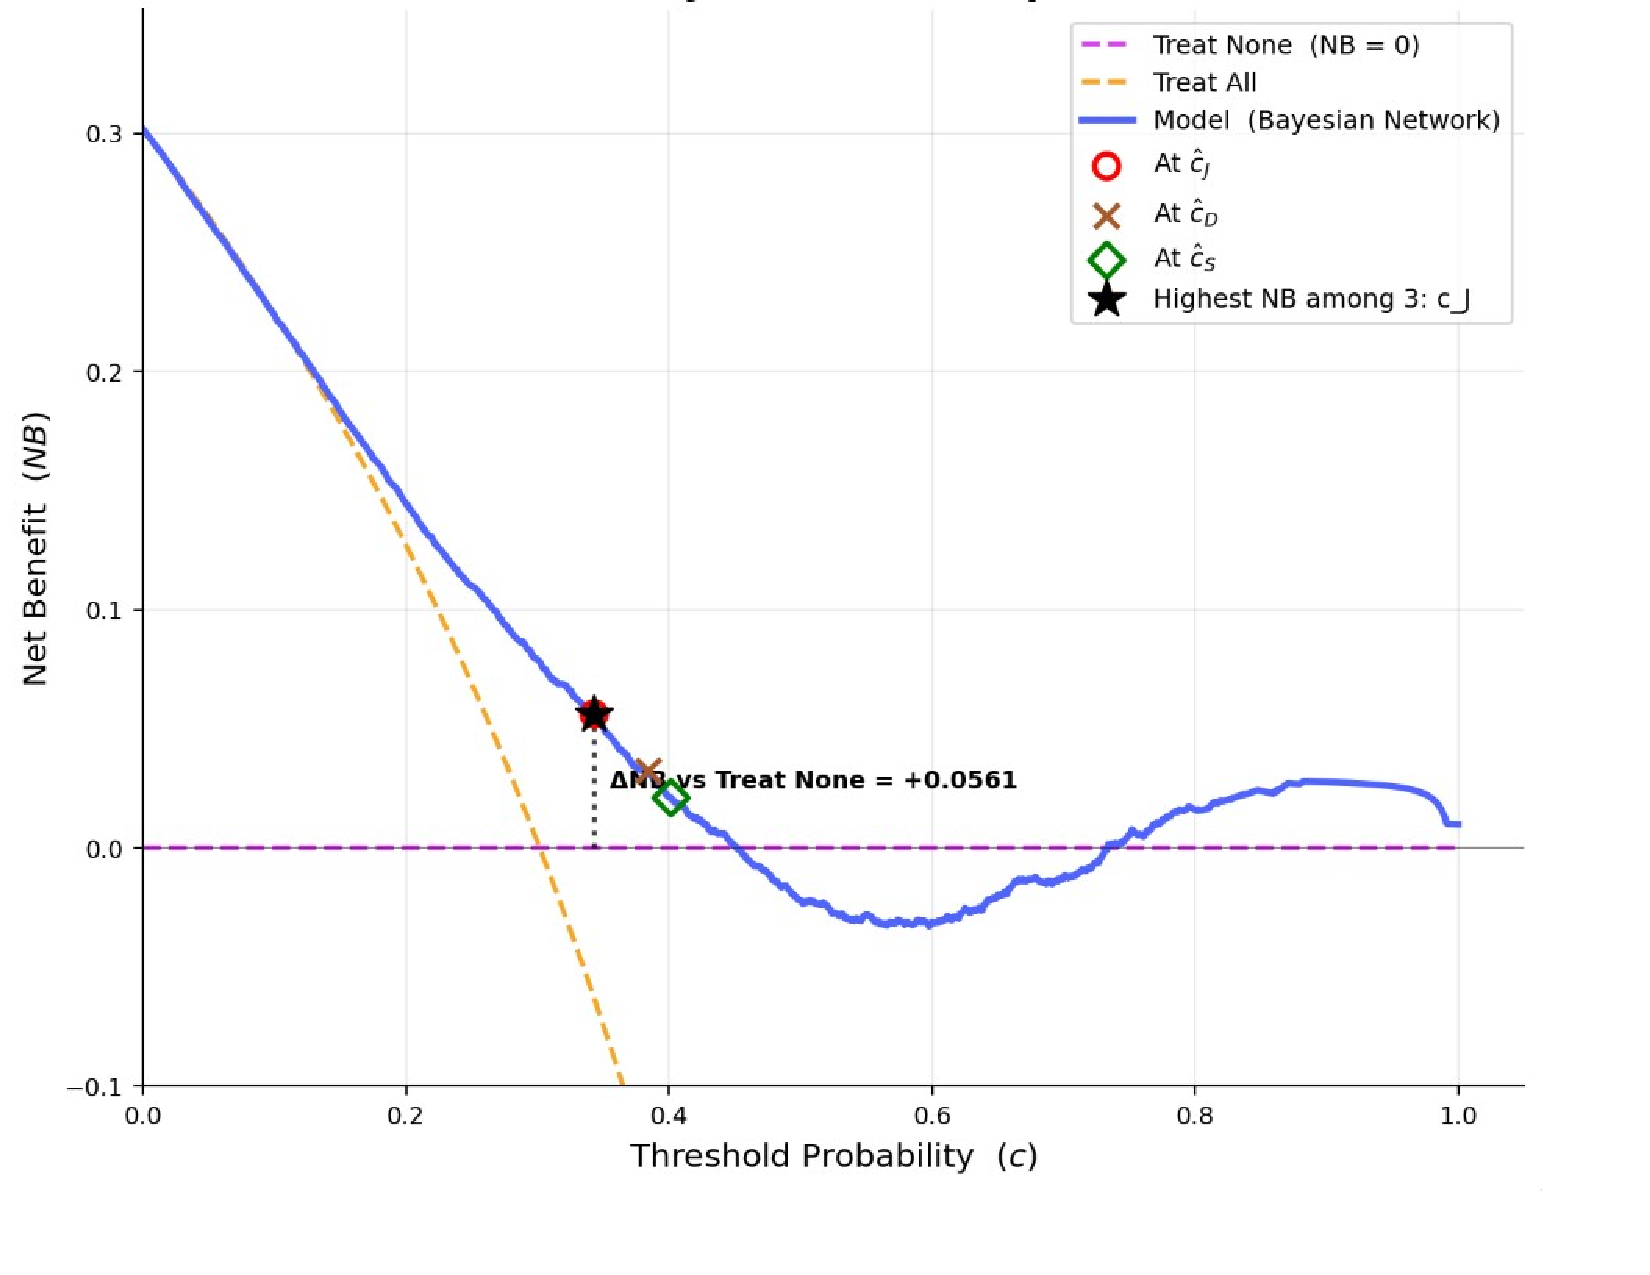
\includegraphics[width=\textwidth]{image/roc_dca/dca_lend.pdf}
    \end{subfigure}
    \caption{Đồ thị ba ngưỡng quyết định tối ưu trên DCA --- Lending Club}
    \label{fig:dca_lend}
\end{figure}

\begin{table}[H]
\centering
\caption{Ba ngưỡng quyết định tối ưu theo ROC -- Lending Club (tập validation)}
\label{tab:roc_threshold_lending}

\renewcommand{\arraystretch}{1.3}

\begin{tabular}{|p{3.5cm}|c|c|c|c|c|}
\hline
\rowcolor{gray!20}
\centering\textbf{Tiêu chí ngưỡng} &
\centering\textbf{Ngưỡng (c)} &
\centering\textbf{Sensitivity} &
\centering\textbf{Specificity} &
\centering\textbf{Accuracy} &
\centering\arraybackslash\textbf{F1-Score} \\
\hline

Youden Index
& 0.3593
& 0.7232
& 0.5313
& 0.5892
& 0.5151 \\
\hline

Closest to (0,1)
& 0.4016
& 0.6403
& 0.6098
& 0.6190
& 0.5035 \\
\hline

Symmetry Point
& 0.4088
& 0.6227
& 0.6227
& 0.6227
& 0.4989 \\
\hline

\end{tabular}
\end{table}
\FloatBarrier

\noindent
Trên bộ Lending Club, khi hạ ngưỡng quyết định từ 0.5 mặc định xuống mức tối ưu theo Youden ($\approx$ 0.3593) làm tăng đáng kể độ nhạy (từ 0.4878 lên 0.7232) nhưng đồng thời làm giảm độ đặc hiệu và độ chính xác tổng thể,  là sự đánh đổi kinh điển (trade-off) giữa việc phát hiện nhiều khách hàng vỡ nợ hơn (giảm rủi ro bỏ sót  FN) với chi phí từ chối oan nhiều khách hàng tốt hơn (tăng FP). Trên Australian Credit, do mô hình đã đạt hiệu năng cao ở ngưỡng mặc định, nên ở ngưỡng tối ưu Youden và Closest-to (0,1) mô hình có hiệu năng trùng khớp nhau hoàn toàn (0.4254 $\approx$ 0.4052, cùng cho Accuracy 0.8551), cho thấy đường cong ROC của bộ dữ liệu này có hình dạng rất gần góc trên bên trái, cho thấy đặc trưng của một bộ phân loại mạnh.

Mô hình BN cho lợi ích ròng dương trên cả ba bộ dữ liệu trong vùng ngưỡng xác suất thấp đến trung bình, vượt trội hơn cả hai chiến lược biên, chứng minh giá trị triển khai thực tiễn của mô hình ngoài giá trị thống kê thuần túy. Đáng chú ý, Net Benefit tuyệt đối tại Australian Credit (0.4661) cao hơn rất nhiều so với German Credit (0.1474) và Lending Club (0.0561), phản ánh trực tiếp hiệu năng phân loại vượt trội của mô hình trên bộ dữ liệu này (ROC-AUC = 0.9220), đồng thời cũng phản ánh prevalence cao hơn (0.58) làm tăng quy mô tuyệt đối của lợi ích ròng có thể đạt được. Sự thay đổi của các chỉ số khi áp dụng các ngưỡng tối ưu trên ba bộ dữ liệu được phản ánh trong Bảng \ref{tab:bn_best_c}.

\vspace{1em}
\begin{table}[ht]
\centering
\caption{So sánh chỉ số đánh giá mô hình mạng Bayes với ngưỡng tối ưu trên tập test}
\label{tab:bn_best_c}

\renewcommand{\arraystretch}{1.3}

\begin{tabular}{|
p{2cm}|
>{\centering\arraybackslash}p{1.2cm}|
>{\centering\arraybackslash}p{2cm}|
>{\centering\arraybackslash}p{1.2cm}|
>{\centering\arraybackslash}p{2cm}|
>{\centering\arraybackslash}p{1.2cm}|
>{\centering\arraybackslash}p{2cm}|}

\hline
\rowcolor{gray!20}

\makecell{\centering \textcolor{black}{\textbf{Chỉ số}}} &
\multicolumn{2}{c|}{\textcolor{black}{\textbf{Australian Credit}}} &
\multicolumn{2}{c|}{\textcolor{black}{\textbf{German Credit}}} &
\multicolumn{2}{c|}{\textcolor{black}{\textbf{Lending Club}}} \\

\cline{2-7}

\rowcolor{gray!20}
&

\multicolumn{1}{>{\columncolor{gray!20}}c|}{\textcolor{black}{\textbf{$c=0.5$}}} &
\multicolumn{1}{>{\columncolor{gray!20}}c|}{\textcolor{black}{\textbf{$c^{*}=0.3818$}}} &
\multicolumn{1}{>{\columncolor{gray!20}}c|}{\textcolor{black}{\textbf{$c=0.5$}}} &
\multicolumn{1}{>{\columncolor{gray!20}}c|}{\textcolor{black}{\textbf{$c^{*}=0.1895$}}} &
\multicolumn{1}{>{\columncolor{gray!20}}c|}{\textcolor{black}{\textbf{$c=0.5$}}} &
\multicolumn{1}{>{\columncolor{gray!20}}c|}{\textcolor{black}{\textbf{$c^{*}=0.3593$}}} \\

\hline

Accuracy
& 0.8406 & 0.8551
& 0.7300 & 0.6750
& 0.6808 & 0.5897 \\

\hline

Precision
& 0.9211 & 0.8367
& 0.6047 & 0.4891
& 0.4610 & 0.3926 \\

\hline

Recall 
& 0.8140 & 0.9535
& 0.4127 & 0.7143
& 0.4878 & 0.7157 \\

\hline

Specificity
& 0.8846 & 0.6923
& 0.8759 & 0.6569
& 0.7615 & 0.5370 \\

\hline

F1-Score
& 0.8642 & 0.8913
& 0.4906 & 0.5806
& 0.4740 & 0.5070 \\

\hline

\end{tabular}
\end{table}


Nền kinh tế Úc vận hành dưới hệ thống Báo cáo tín dụng toàn diện (Comprehensive Credit Reporting - CCR) \cite{Australia2021MandatoryCCR}. Trước đây, Úc dùng hệ thống báo cáo tiêu cực (chỉ ghi nhận nợ xấu), nhưng hệ thống CCR hiện tại bắt buộc các ngân hàng chia sẻ cả dữ liệu tích cực (lịch sử đóng tiền đúng hạn 24 tháng, hạn mức tín dụng, hành vi thanh toán thực tế). Nhờ có cơ sở dữ liệu hai chiều (tích cực + tiêu cực) phong phú từ hệ thống CCR, mô hình máy học có đủ các đặc trưng chất lượng để bóc tách một cách mượt mà và chính xác nhóm khách hàng rủi ro \cite{Treasury2023CCR}. Sự minh bạch thông tin giúp đường DCA của mô hình nới rộng khoảng cách tối đa với đường Treat All.

Nền văn hóa tài chính Đức nổi tiếng thế giới vì tính thận trọng, kỷ luật và cực kỳ bài xích rủi ro (risk-averse) \cite{BundesbankCash}. Người dân Đức có tỷ lệ tích lũy tài sản cao, chuộng dùng tiền mặt hoặc thẻ ghi nợ và rất hạn chế vay tiêu dùng qua thẻ tín dụng \cite{BundesbankCash}. Hệ thống chấm điểm tín dụng quốc gia Đức bị chi phối bởi tập đoàn SCHUFA. Tiêu chí chấm điểm của SCHUFA đặt trọng số cực kỳ nặng nề lên các yếu tố tiêu cực (lịch sử trễ hạn, hồ sơ đòi nợ, phá sản cá nhân) \cite{ECJ2023SCHUFA}. Những người không có "vết đen" mặc định được coi là có uy tín rất cao. Do quy trình sàng lọc sơ bộ của các ngân hàng Đức kết hợp với hệ thống SCHUFA quá chặt chẽ, tệp khách hàng vượt qua vòng gửi xe để tiến vào mô hình chấm điểm chuyên sâu phần lớn là những hồ sơ cực kỳ sạch, dẫn đến tỷ lệ nợ xấu tự nhiên (default base rate) trong tập dữ liệu ở mức siêu thấp \cite{WorldBankNPLGermany}. Thị trường Đức thiên hẳn về chiến lược Recall (Ưu tiên tối đa) với tư duy cốt lõi: "Thà từ chối nhầm khách hàng tốt còn hơn để lọt một khoản nợ xấu". Điểm tối ưu của họ nằm ở một ngưỡng xác suất rất thấp ($\hat{c}_D \approx 0.19$), nghĩa là chỉ cần mô hình phát hiện một tia rủi ro nhỏ, họ lập tức từ chối vay. Nếu cố tình tăng ngưỡng xác suất lên cao để cố cứu vãn khách hàng (tăng Precision), lợi ích ròng lập tức sụt giảm nghiêm trọng và rơi xuống vùng âm do vi phạm quy chuẩn an toàn khắt khe của hệ thống tài chính Đức.

Lending Club không phải ngân hàng thương mại truyền thống mà khởi thân là một nền tảng cho vay ngang hàng / Fintech tại Mỹ, chuyên cung cấp các khoản vay cá nhân tín chấp (unsecured personal loans) \cite{LendingClub10K}. Trong một môi trường cho vay tín chấp rủi ro cao như P2P, nếu áp dụng chiến lược "Treat All" (cho vay đại trà) thì dòng tiền bùng nợ sẽ lập tức thổi bay toàn bộ nguồn vốn, gây lỗ nặng cho nhà đầu tư (đường Treat All lao dốc âm sâu) \cite{SerranoCinca2016}. Do đó, điểm neo an toàn tối thiểu của họ phải là "Treat None" (giữ tiền mặt, không làm gì để bảo toàn vốn). Họ cần đảm bảo những hồ sơ được dán nhãn "Tốt" và phê duyệt phải có độ chính xác cao nhằm bảo vệ lợi nhuận và duy trì niềm tin bền vững cho các nhà đầu tư góp vốn trên nền tảng.

\subsubsection{So sánh mạng Bayes với các mô hình máy học đối chứng}

Trên bộ Australian Credit (Hình \ref{fig:auc_au} và Bảng \ref{tab:compare_australian}), BN đạt ROC-AUC (0.9220) và PR-AUC (0.9371) cao nhất trong toàn bộ các mô hình được thử nghiệm, kể cả Stacking Ensemble. Đây là kết quả nổi bật nhất của BN trong cả ba bộ dữ liệu, cho thấy với bộ dữ liệu nhỏ, ít đặc trưng và cấu trúc nhân quả tương đối rõ ràng, mạng Bayes có lợi thế vượt trội so với cả các mô hình ensemble phức tạp hơn.

\begin{figure}[H]
    \centering
    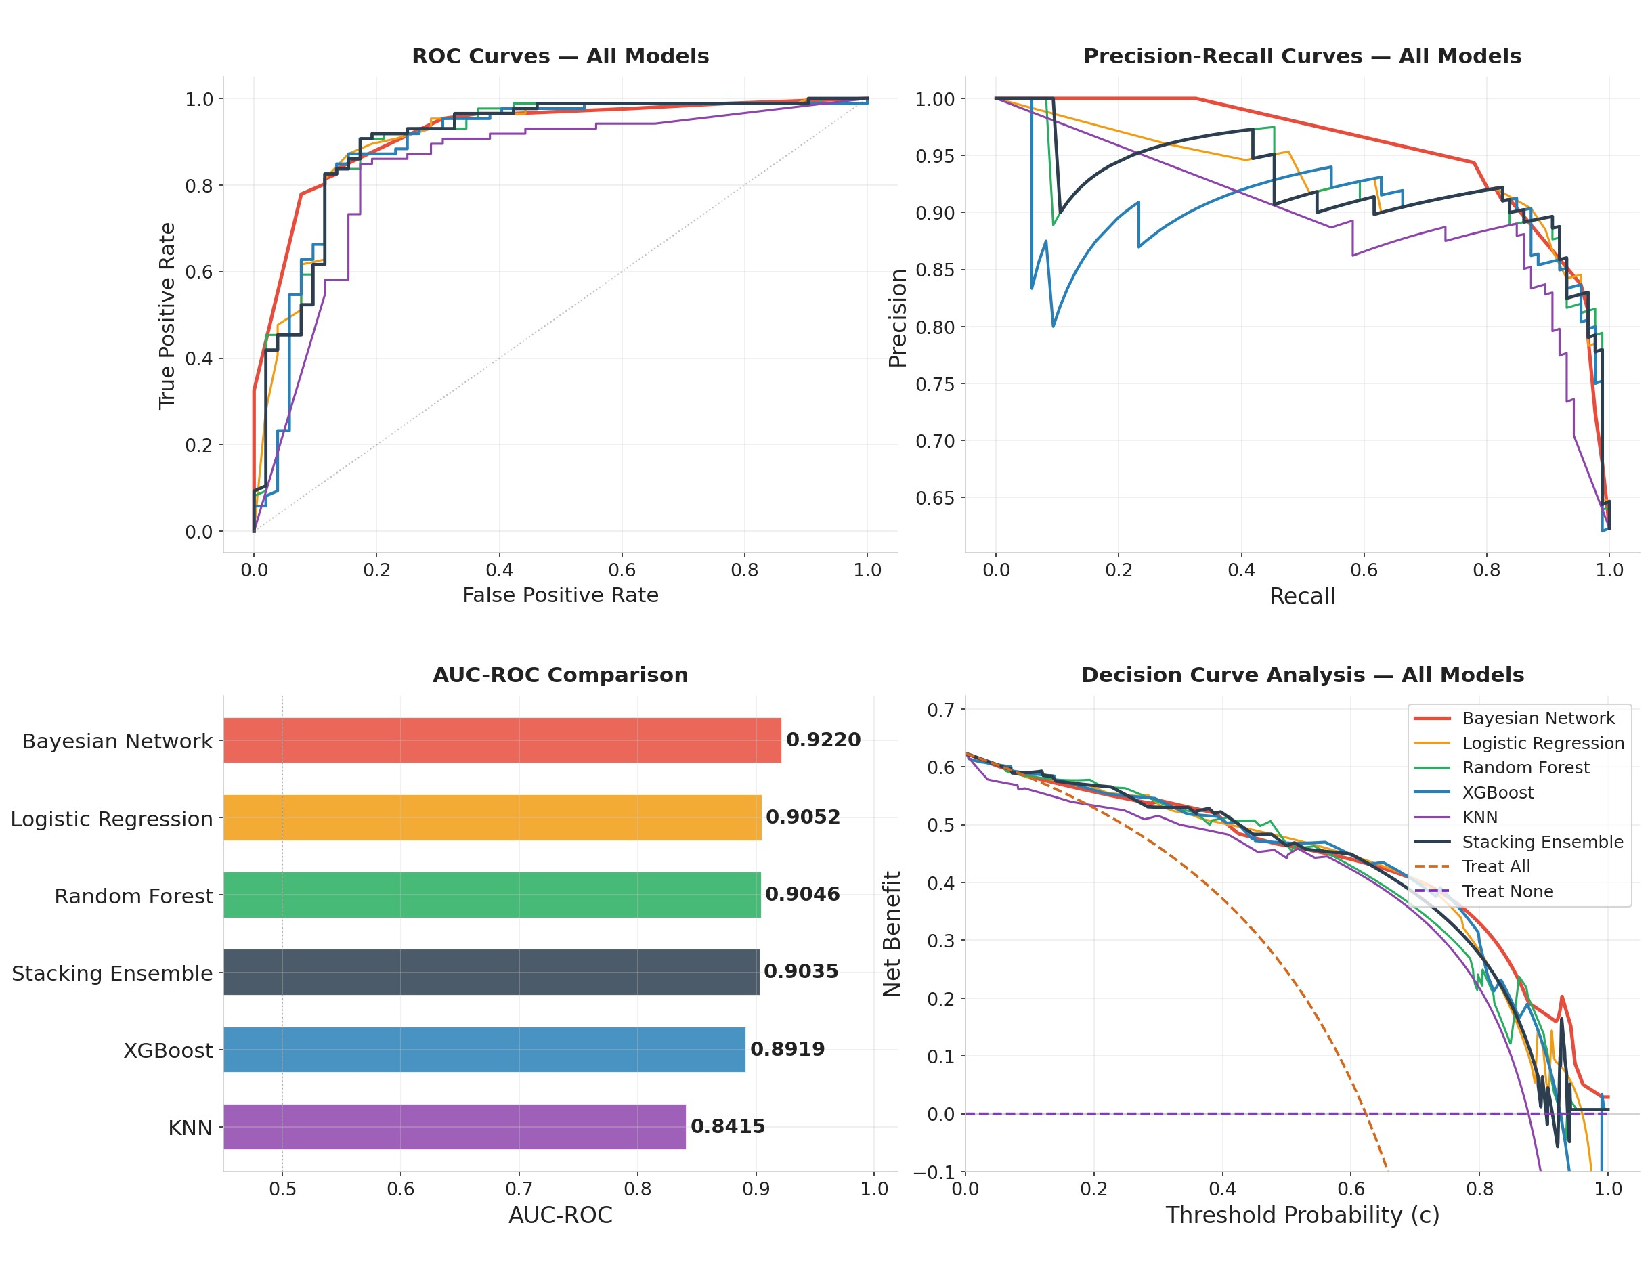
\includegraphics[width=1\textwidth]{image/allmodel/model_au.pdf}
    \caption{So sánh hiệu năng của mô hình mạng Bayes với các mô hình máy học trên bộ dữ liệu Australian Credit}
    \label{fig:auc_au}
\end{figure}
\FloatBarrier

\begin{table}[H]
\centering
\caption{So sánh hiệu năng các mô hình trên Australian Credit}
\label{tab:compare_australian}

\renewcommand{\arraystretch}{1.3}

\begin{tabular}{|p{4cm}|c|c|}
\hline
\rowcolor{gray!20}
\centering\textbf{Mô hình} &
\centering\textbf{ROC-AUC} &
\centering\arraybackslash\textbf{PR-AUC} \\
\hline

Bayesian Network  & 0.9220 & 0.9371 \\
\hline
Logistic Regression & 0.9052 & 0.9218 \\
\hline
Random Forest & 0.9046 & 0.9238 \\
\hline
XGBoost & 0.8919 & 0.8997 \\
\hline
KNN & 0.8415 & 0.8633 \\
\hline
Stacking Ensemble & 0.9055 & 0.9233 \\
\hline

\end{tabular}
\end{table}


\begin{figure}[H]
    \centering
    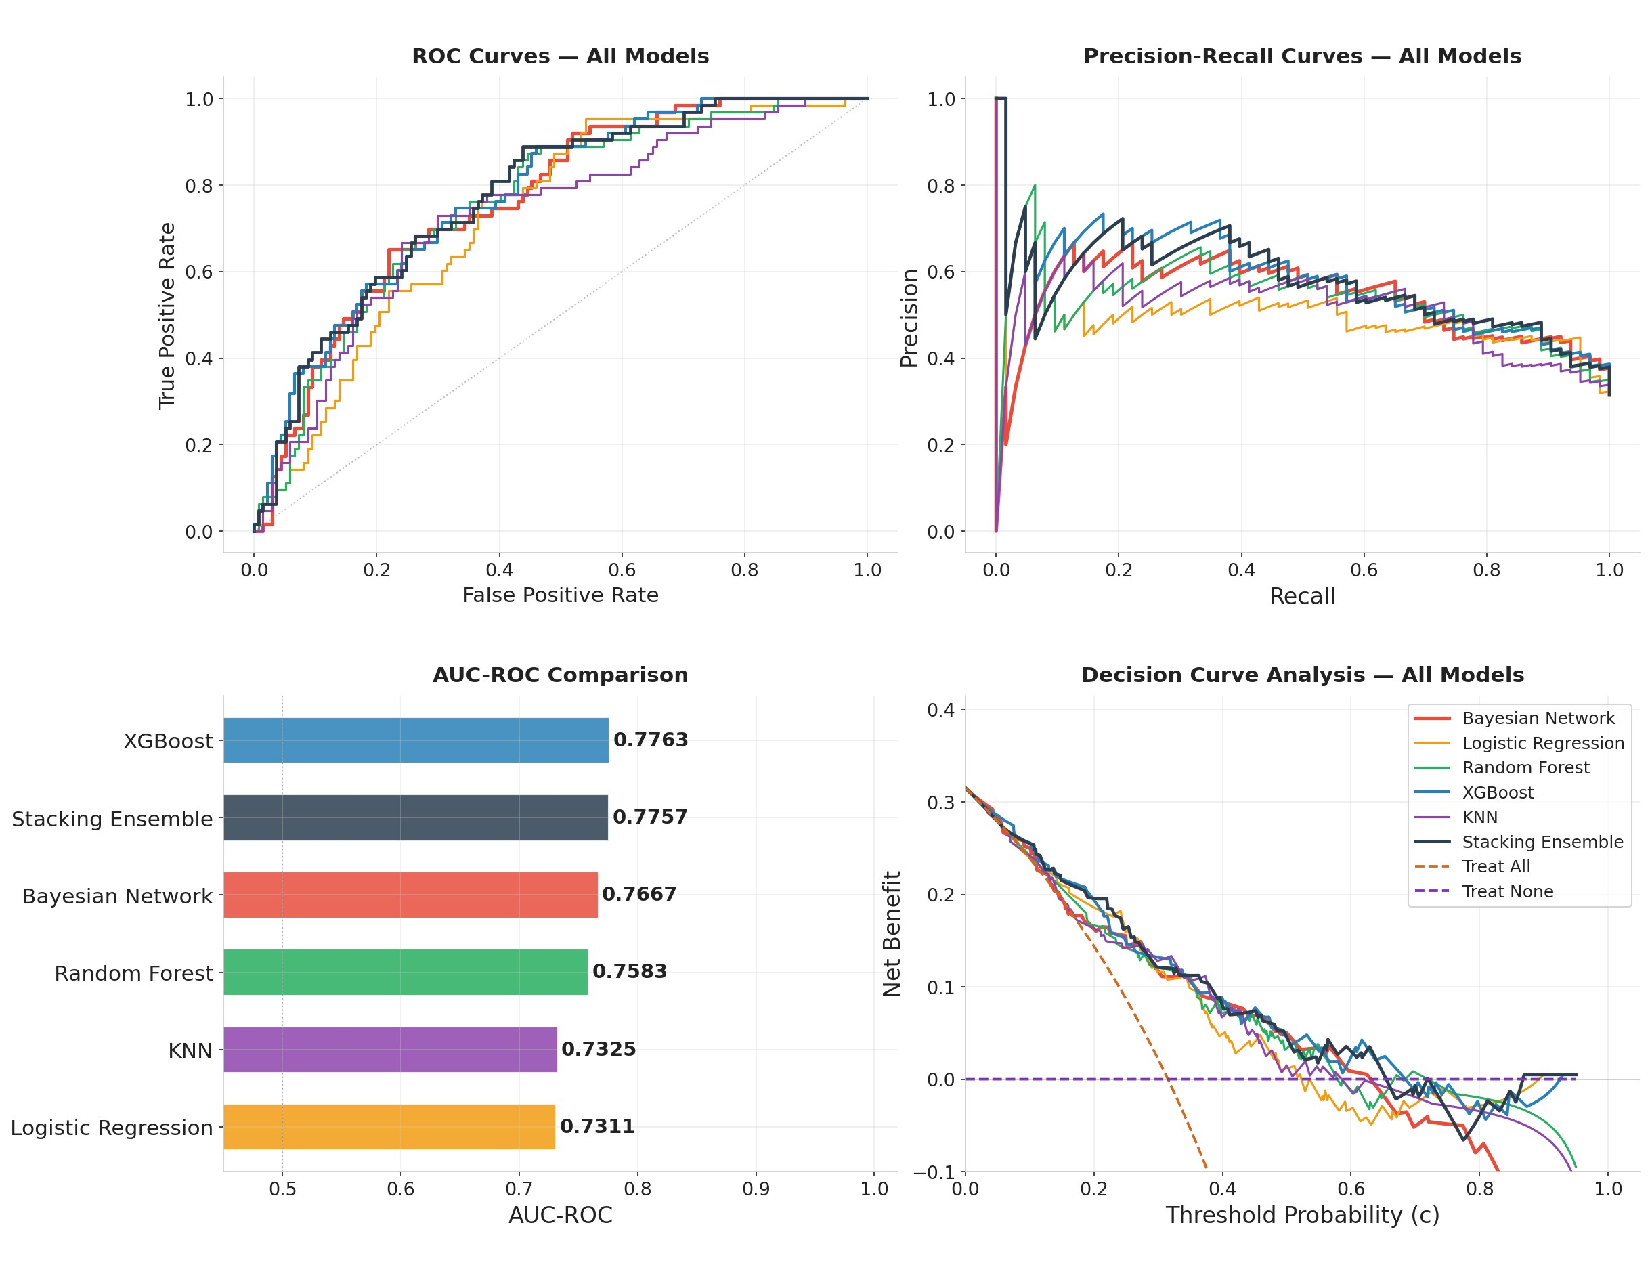
\includegraphics[width=1\textwidth]{image/allmodel/model_ger.pdf}
    \caption{So sánh hiệu năng của mô hình mạng Bayes với các mô hình máy học trên bộ dữ liệu German Credit}
    \label{fig:auc_ger}
\end{figure}


\begin{table}[h]
\centering
\caption{So sánh hiệu năng các mô hình trên German Credit}
\label{tab:compare_german}

\renewcommand{\arraystretch}{1.3}

\begin{tabular}{|p{4cm}|c|c|}
\hline
\rowcolor{gray!20}
\centering\textbf{Mô hình} &
\centering\textbf{ROC-AUC} &
\centering\arraybackslash\textbf{PR-AUC} \\
\hline

Bayesian Network & 0.7667 & 0.5421 \\
\hline
Logistic Regression & 0.7311 & 0.5015 \\
\hline
Random Forest & 0.7583 & 0.5433 \\
\hline
XGBoost & 0.7763 & 0.5888 \\
\hline
KNN & 0.7325 & 0.5172 \\
\hline
Stacking Ensemble & 0.7757 & 0.5785 \\
\hline

\end{tabular}
\end{table}

Trên German Credit (Hình \ref{fig:auc_ger} và Bảng \ref{tab:compare_german}), ROC-AUC = 0.7667 của mạng Bayes vượt trội hơn Logistic Regression, Random Forest và KNN, nhưng thấp hơn nhẹ so với XGBoost (0.7763) và Stacking Ensemble (0.7757).


\begin{figure}[H]
    \centering
    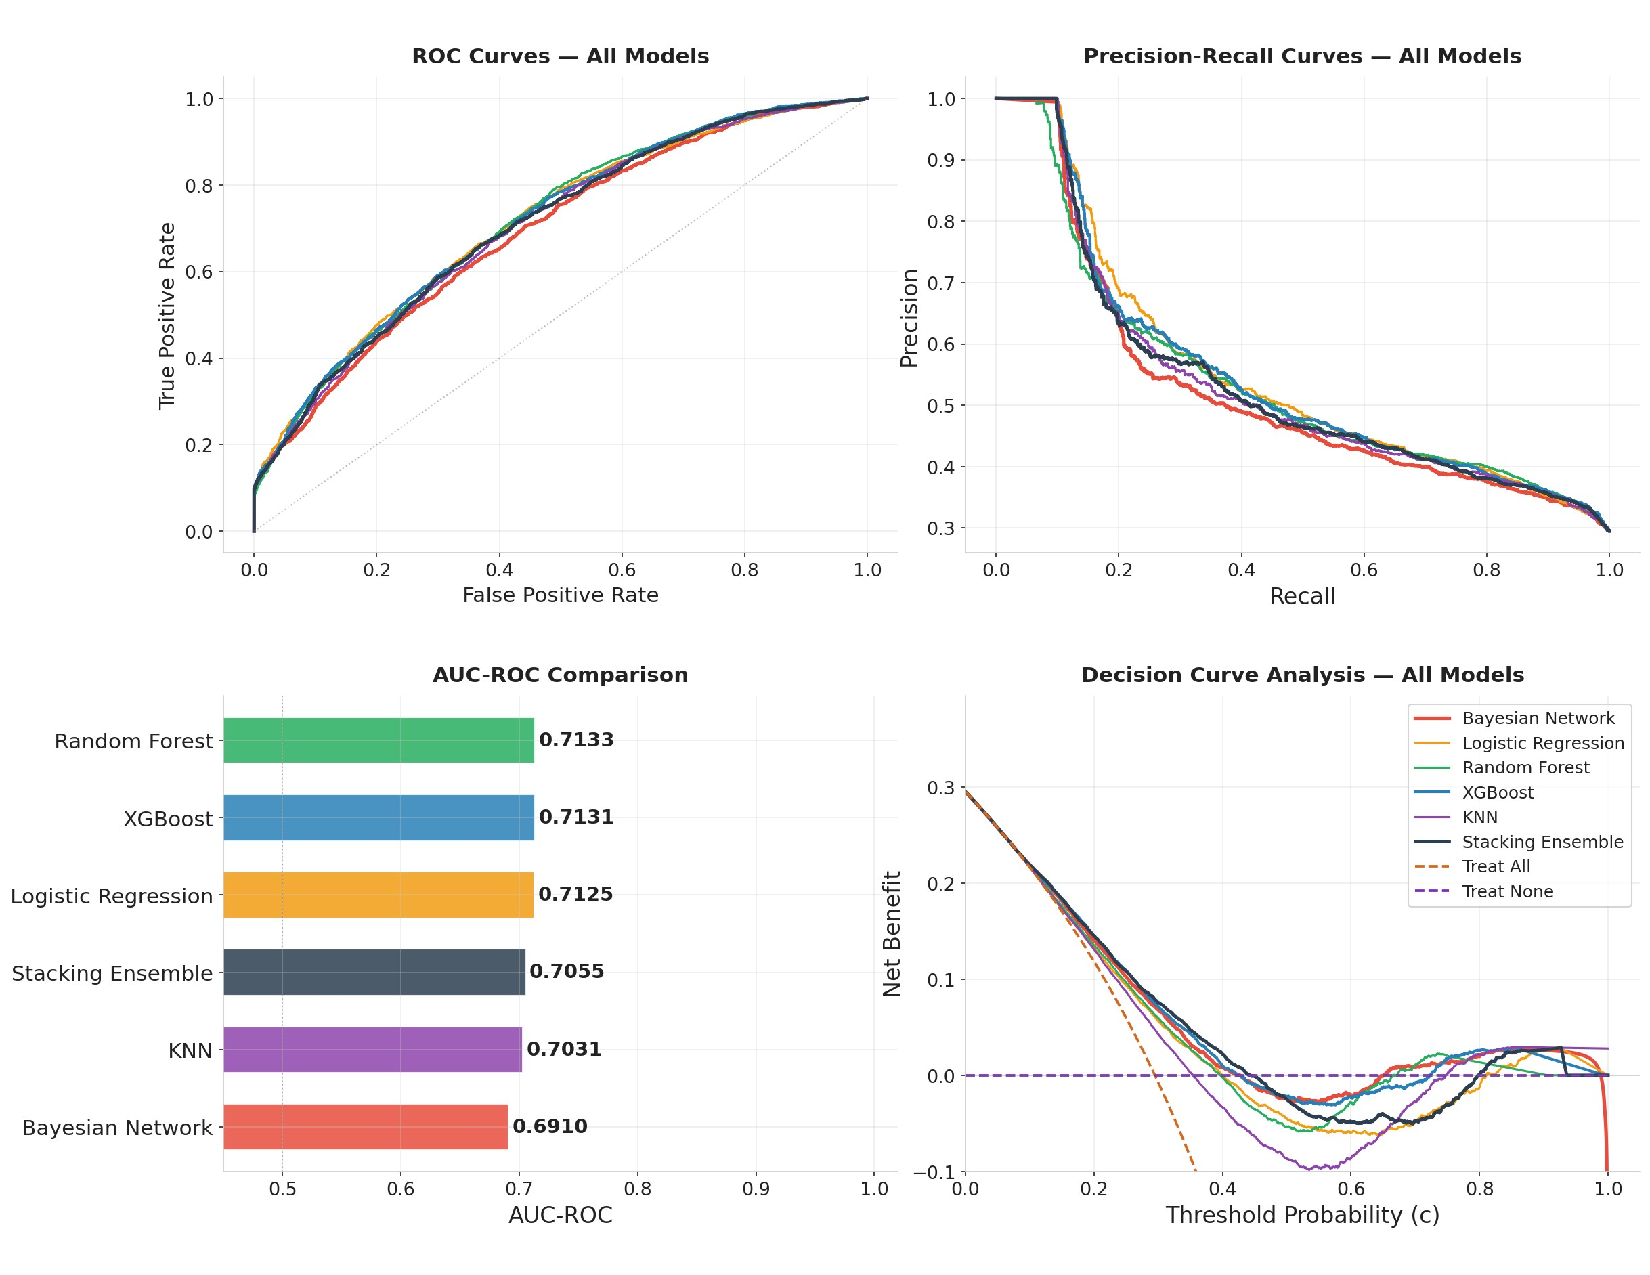
\includegraphics[width=1\textwidth]{image/allmodel/model_lend.pdf}

    \caption{So sánh hiệu năng của mô hình mạng Bayes với các mô hình máy học trên bộ dữ liệu Lending Club}
    \label{fig:auc_lend}
\end{figure}

\begin{table}[h]
\centering
\caption{So sánh hiệu năng các mô hình trên Lending Club}
\label{tab:compare_lending}
\renewcommand{\arraystretch}{1.3}

\begin{tabular}{|p{4cm}|c|c|}
\hline
\rowcolor{gray!20}
\centering\textbf{Mô hình} &
\centering\textbf{ROC-AUC} &
\centering\arraybackslash\textbf{PR-AUC} \\
\hline

Bayesian Network & 0.6910 & 0.5224 \\
\hline
Logistic Regression & 0.7125 & 0.5528 \\
\hline
Random Forest & 0.7133 & 0.5395 \\
\hline
XGBoost & 0.7131 & 0.5483 \\
\hline
KNN & 0.7031 & 0.5352 \\
\hline
Stacking Ensemble & 0.7055 & 0.5371 \\
\hline

\end{tabular}
\end{table}

\FloatBarrier

Ngược lại, trên bộ dữ liệu Lending Club (Hình \ref{fig:auc_lend} và Bảng \ref{tab:compare_lending}) quy mô lớn, BN có ROC-AUC thấp nhất (0.6910) trong số sáu mô hình, đứng sau cả bốn mô hình máy học đơn lẻ và Stacking Ensemble. Sự sụt giảm tương đối này phù hợp với nhận định khi số chiều đặc trưng và độ phức tạp cấu trúc DAG tăng (28 node, 58 cạnh), suy diễn xác suất chính xác của BN gặp khó khăn hơn so với các mô hình boosting/ensemble vốn linh hoạt hơn trong việc nắm bắt tương tác phi tuyến giữa nhiều đặc trưng.

Kết quả so sánh cho thấy một phát hiện thực nghiệm có ý nghĩa quan trọng đối với luận điểm của bài nghiên cứu: vị thế tương đối của mạng Bayes so với các mô hình máy học hiện đại (XGBoost, Random Forest) không cố định mà phụ thuộc mạnh vào đặc điểm dữ liệu. Trên bộ dữ liệu lớn, nhiều đặc trưng và nhiều nhiễu (Lending Club), BN xếp hạng cuối cùng (hạng 6/6), phản ánh hạn chế cố hữu của mạng Bayes rời rạc khi phải xử lý không gian đặc trưng lớn: việc rời rạc hóa biến liên tục gây mất thông tin, và CPT với nhiều tổ hợp trạng thái dễ rơi vào tình trạng ước lượng tham số kém chính xác do dữ liệu thưa trên mỗi ô tổ hợp. Trên German Credit (quy mô trung bình), BN vươn lên hạng 3/6, vượt qua cả Random Forest, KNN và Logistic Regression, chỉ thua Stacking Ensemble và XGBoost với khoảng cách rất nhỏ (dưới 1 điểm phần trăm). Đặc biệt, trên Australian Credit (quy mô nhỏ, ít đặc trưng), BN đạt vị trí dẫn đầu tuyệt đối (hạng 1/6) ở cả hai chỉ số AUC-ROC (0.9220) và AUC-PR (0.9371), vượt qua toàn bộ mô hình đối chứng bao gồm cả Stacking Ensemble, minh chứng rõ ràng cho việc cấu trúc đồ thị xác suất tường minh của BN phát huy lợi thế tối đa khi số lượng biến nhỏ và mối quan hệ nhân quả giữa các biến đơn giản.

\subsection{Suy luận nhân quả (In\_Pro)}
\noindent
Bốn kỹ thuật diễn giải được triển khai tuần tự trên cả ba bộ dữ liệu Australian Credit, German Credit và Lending Club, bao gồm phân tích độ nhạy tham số kết hợp thông tin tương hỗ, suy luận tiến, suy luận lùi kết hợp phân tích kịch bản giả định, và cuối cùng là đối chiếu với hai phương pháp diễn giải hậu kiểm phổ biến là LIME và SHAP. Cách tiếp cận này bám sát khung lý thuyết của Liu và cộng sự \cite{liu2024credit}, theo đó bốn kỹ thuật trên được xem là bốn góc nhìn bổ trợ lẫn nhau để khai thác trọn vẹn khả năng diễn giải nội tại của mạng Bayes, thay vì chỉ dừng lại ở một phép đo đơn lẻ.

\subsubsection{Phân tích độ nhạy}
\label{sec:4.4.1}
\noindent
Áp dụng phương pháp đã trình bày ở Mục \ref{sec: 3.3.3}, nghiên cứu thực nghiệm $\delta$ và thông tin tương hỗ trên cả ba bộ dữ liệu bằng \texttt{pgmpy} và \texttt{scikit-learn}, giới hạn phạm vi khảo sát $\delta$ trong tập biến thuộc Markov Blanket của \texttt{target}.

Đối với Australian Credit, Markov Blanket của \texttt{target} chỉ gồm ba biến \texttt{CreditHistory}, \texttt{Income} và \texttt{Employed}, đúng như cấu trúc đồ thị gọn nhẹ đã ghi nhận tại Mục \ref{sec: 4.3.1}, với $\max|\delta|$ lần lượt là $0.4249$; $0.2871$ và $0.2545$ ở Hình \ref{fig:sens_au}. \texttt{CreditHistory} thể hiện quan hệ đơn điệu rõ ràng tại Hình \ref{fig:prob_au}: khách hàng không có lịch sử tín dụng mang xác suất vỡ nợ $92.5\%$, trong khi khách hàng đã có lịch sử tín dụng giảm mạnh xuống còn $18.3\%$, phản ánh đúng vai trò của biến này như một chỉ báo uy tín nền tảng. Ngược lại, \texttt{Income} không biểu hiện quan hệ đơn điệu qua bốn bin: xác suất vỡ nợ tăng từ $60.1\%$ ở bin thấp nhất lên đỉnh $69.3\%$ ở bin thứ hai, trước khi giảm dần còn $50.2\%$ và $21.3\%$ ở hai bin cao nhất. Hiện tượng phản trực giác này có thể xuất phát từ việc xác suất hậu nghiệm của \texttt{Income} đã được tích hợp qua toàn bộ cấu trúc phụ thuộc với \texttt{CreditHistory} và \texttt{Employed} trong Markov Blanket, khiến một bin thu nhập cụ thể trùng lặp cao với nhóm khách hàng thiếu lịch sử tín dụng hoặc chưa có việc làm ổn định; quy mô mẫu nhỏ của bộ dữ liệu này cũng làm một số bin sau rời rạc hóa dễ bị nhiễu thống kê hơn.

\vspace{1em}
% =========================================================================
% KHỐI HÌNH 4.7 - PHẦN 1: Australian Credit (lấp khoảng trống còn lại)
% =========================================================================
\begin{figure}[H]
    \centering
    \begin{subfigure}[b]{\textwidth}
        \centering
        \begin{minipage}{0.75\textwidth}
            \centering
            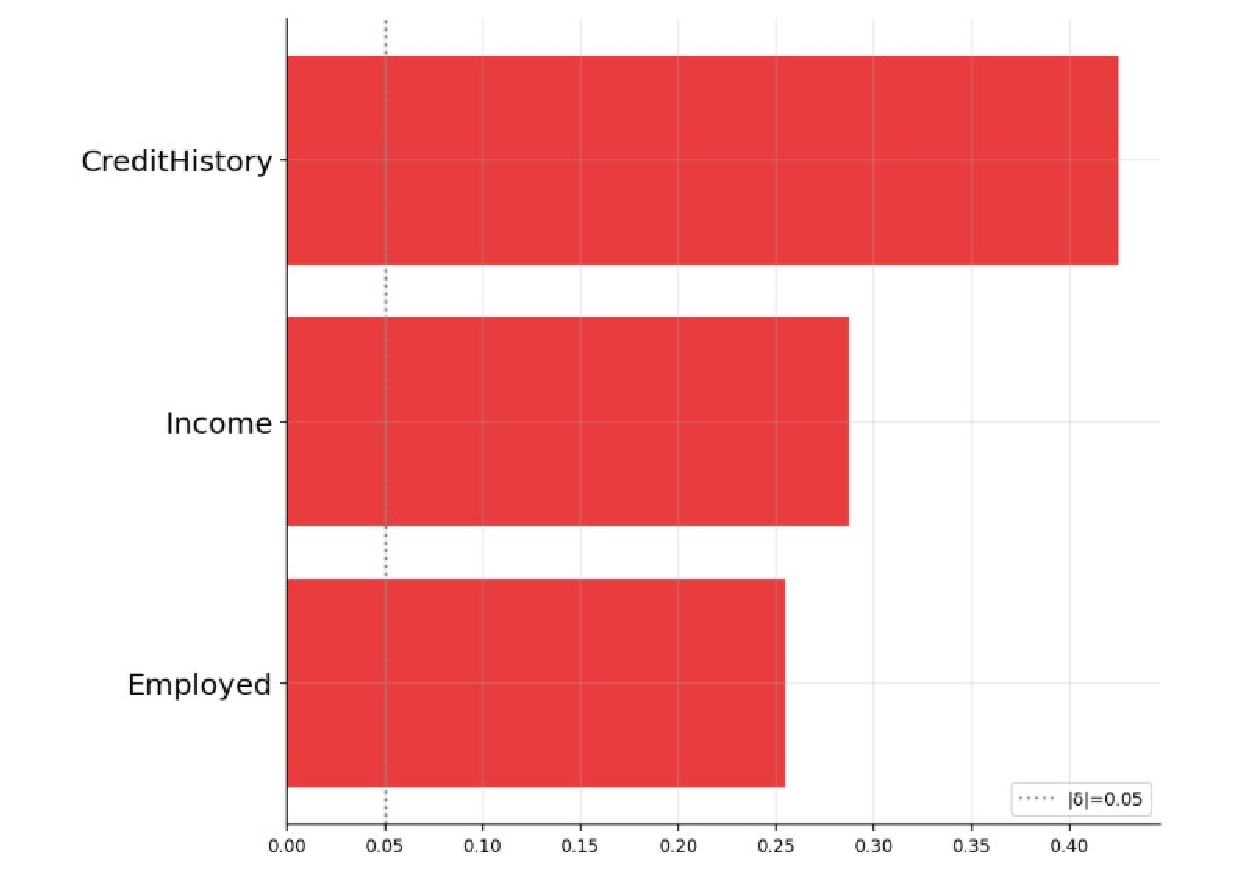
\includegraphics[width=\textwidth]{image/sensitivity/11_sensitivity_au.pdf}\\[0.1cm]
            {\small Biểu đồ độ nhạy ($\delta$)}
        \end{minipage}
        \vspace{0.3cm}
        \begin{minipage}{0.8\textwidth}
            \centering
            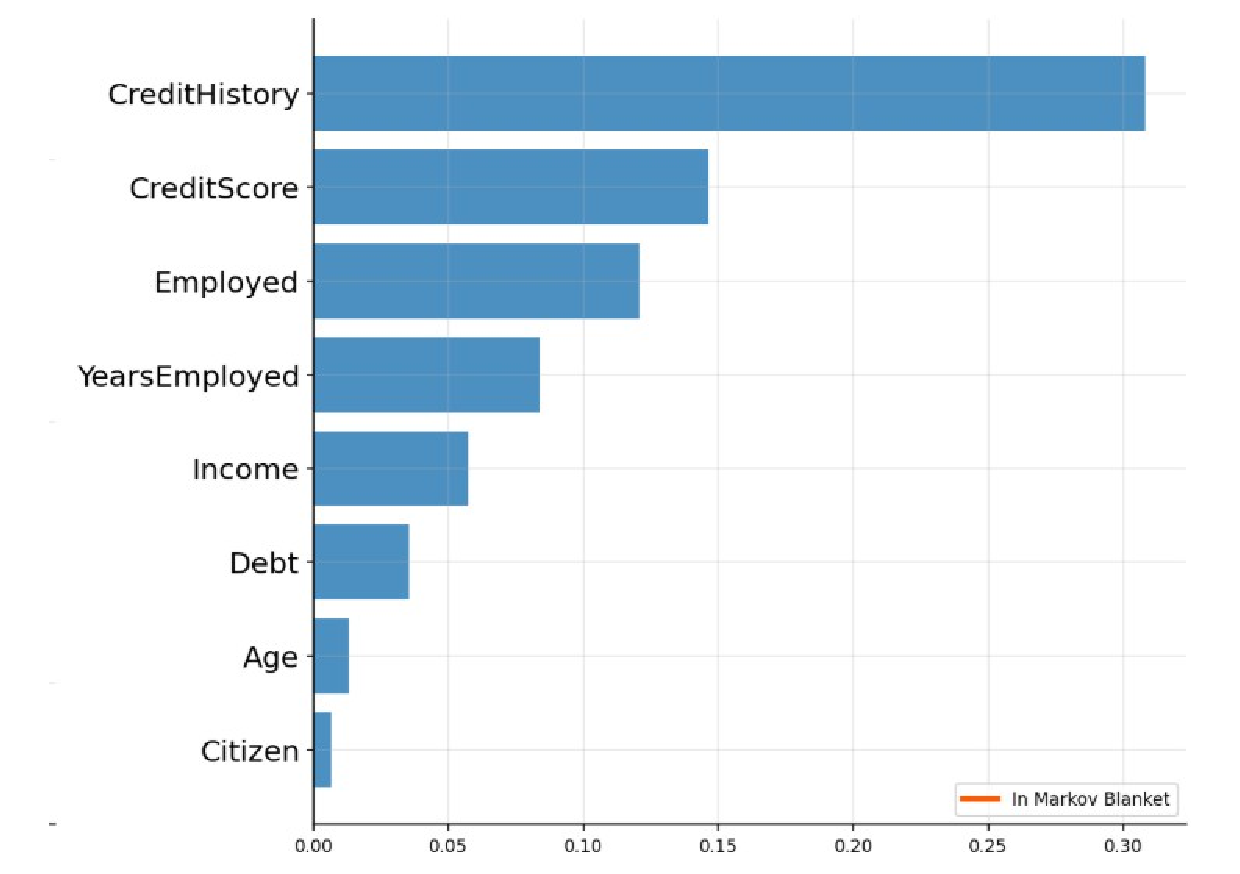
\includegraphics[width=\textwidth]{image/sensitivity/12_sensitivity_au.pdf}\\[0.1cm]
            {\small Thông tin tương hỗ}
        \end{minipage}    
    \end{subfigure}
    \caption{Biểu đồ độ nhạy ($\delta$) và thông tin tương hỗ trên tập biến thuộc Markov Blanket --- Australian Credit}
    \label{fig:sens_au}
\end{figure}
\FloatBarrier

Trên German Credit, Markov Blanket mở rộng lên 11 biến, dẫn đầu về $\delta$ lần lượt là \texttt{job} ($0.4114$), \texttt{purpose} ($0.3667$), \texttt{other\_installment\_plans} ($0.3614$), \texttt{month\_duration} ($0.3600$), \texttt{is\_foreign\_worker} ($0.3592$), \texttt{credit\_history} ($0.3537$), \texttt{secondary\_obligor} ($0.3430$), \texttt{status\_and\_sex} ($0.2882$), \texttt{status\_account} ($0.2115$), \texttt{collateral} ($0.0936$) và \texttt{housing} ($0.0838$) ở Hình \ref{fig:sens_ger}. Đáng chú ý, thứ hạng theo $\delta$ không trùng khớp với thứ hạng theo thông tin tương hỗ: biến có thông tin tương hỗ cao nhất với \texttt{target} là \texttt{secondary\_obligor}, theo sau là \texttt{other\_installment\_plans} và \texttt{purpose}, trong khi \texttt{job} dẫn đầu về $\delta$ chỉ xếp thứ bảy trên trục thông tin tương hỗ, cho thấy hai chỉ số này đang phản ánh hai khía cạnh khác nhau của mối liên hệ giữa biến và \texttt{target} trên cùng một mạng. Xét chi tiết hai biến nhạy nhất tại Hình \ref{fig:prob_ger}, \texttt{is\_foreign\_worker} cho thấy khách hàng là lao động nước ngoài mang xác suất vỡ nợ $85.9\%$, cao hơn đáng kể so với $42.7\%$ của nhóm không phải lao động nước ngoài. \texttt{other\_installment\_plans} lại cho kết quả phi tuyến tương tự \texttt{Income} ở Australian Credit: nhóm có khoản trả góp tại ngân hàng khác mang xác suất $70.8\%$, nhóm có khoản trả góp tại cửa hàng giảm còn $37.8\%$, nhưng nhóm không có bất kỳ khoản trả góp nào khác lại đạt xác suất cao nhất $86.1\%$, nhiều khả năng do trùng lặp với nhóm có \texttt{status\_account} hoặc \texttt{credit\_history} bất lợi trong Markov Blanket, hơn là do bản thân việc không có khoản vay phụ mang ý nghĩa rủi ro độc lập.

Trên Lending Club, Markov Blanket gồm 15 biến, tương ứng với DAG 58 cạnh đã ghi nhận tại Bảng \ref{tab:result_dag}. Ở Hình \ref{fig:sens_lend}, \texttt{debt\_settlement\_flag} và \texttt{num\_accts\_ever\_120\_pd} đạt $\delta = 0.5000$, khả năng phản ánh hiện tượng dữ liệu thưa tương tự trường hợp \texttt{revol\_util} đã ghi nhận ở Mục \ref{sec: 4.2.5}, hơn là một hiệu ứng nhân quả tuyệt đối, và cần được diễn giải thận trọng. Theo sau là \texttt{grade} ($0.3395$), \texttt{int\_rate} ($0.2746$), \texttt{purpose} ($0.2435$), \texttt{fico\_range\_low} ($0.1486$), \texttt{home\_ownership} ($0.1465$) và \texttt{term} ($0.1392$); trong đó \texttt{grade} và \texttt{int\_rate} cũng đồng thời là hai biến dẫn đầu về thông tin tương hỗ trong cùng biểu đồ. Các biến còn lại như \texttt{acc\_open\_past\_24mths}, \texttt{inq\_last\_6mths}, \texttt{loan\_amnt}, \texttt{mths\_since\_recent\_inq}, \texttt{tot\_cur\_bal}, \texttt{num\_actv\_rev\_tl} và \texttt{mort\_acc} đều có $\max|\delta|$ dưới ngưỡng $0.1$, thể hiện mức độ tác động không đáng kể đến xác suất vỡ nợ so với nhóm biến kể trên. Xét chi tiết hai biến dẫn đầu ở Hình \ref{fig:prob_lend}, xác suất vỡ nợ theo \texttt{grade} tăng từ $16.1\%$ ở hạng tín dụng cao nhất lên $67.4\%$ ở hạng gần thấp nhất, sau đó dao động nhẹ quanh $65\%$--$67\%$ ở hai hạng thấp nhất, cho thấy hiệu ứng biên giảm dần khi khách hàng đã rơi vào nhóm rủi ro cao. Đối với \texttt{int\_rate}, xác suất vỡ nợ tăng đơn điệu và gần như tuyến tính từ $22.5\%$ ở bin lãi suất thấp nhất lên $69.1\%$ ở bin cao nhất.

Tổng hợp trên cả ba bộ dữ liệu, các đặc trưng phản ánh trực tiếp lịch sử tín dụng và định giá rủi ro của bên cho vay (\texttt{CreditHistory}, \texttt{credit\_history}, \texttt{grade}, \texttt{int\_rate}) luôn nằm trong nhóm dẫn đầu về mức độ tác động đến xác suất vỡ nợ, phù hợp với trực giác chuyên gia tín dụng truyền thống. Việc đối chiếu $\delta$ với thông tin tương hỗ còn giúp nhận diện các trường hợp mà biên độ dịch chuyển xác suất lớn không đến từ một mối quan hệ nhân quả bền vững mà từ hiện tượng dữ liệu thưa hoặc hiệu ứng nhiễu qua cấu trúc mạng, một khả năng chẩn đoán mà các phương pháp diễn giải hậu kiểm dạng khép kín khó có thể cung cấp trực tiếp.

\begin{figure}[H]
    \centering
    \begin{subfigure}[b]{\textwidth}
        \centering
        \begin{minipage}{0.9\textwidth}
            \centering
            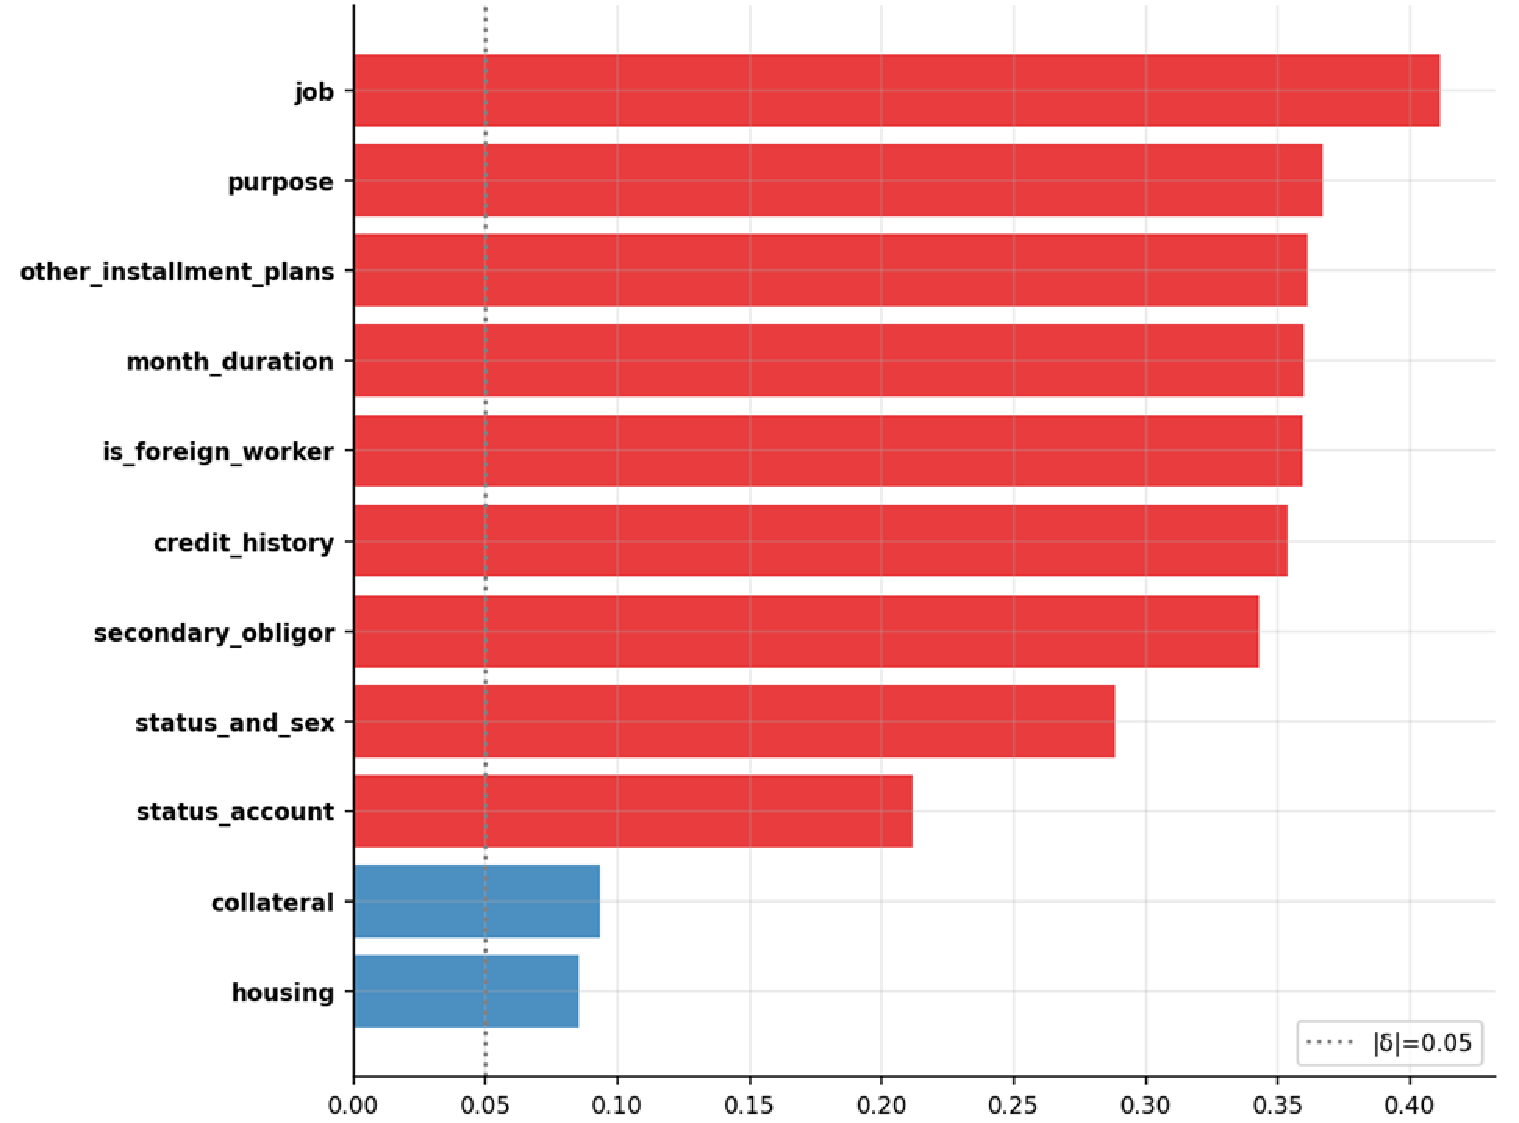
\includegraphics[width=\textwidth]{image/sensitivity/11_sensitivity_ger.pdf}\\[0.1cm]
            {\small Biểu đồ độ nhạy ($\delta$)}
        \end{minipage}
        \vspace{0.3cm}
        \begin{minipage}{0.9\textwidth}
            \centering
            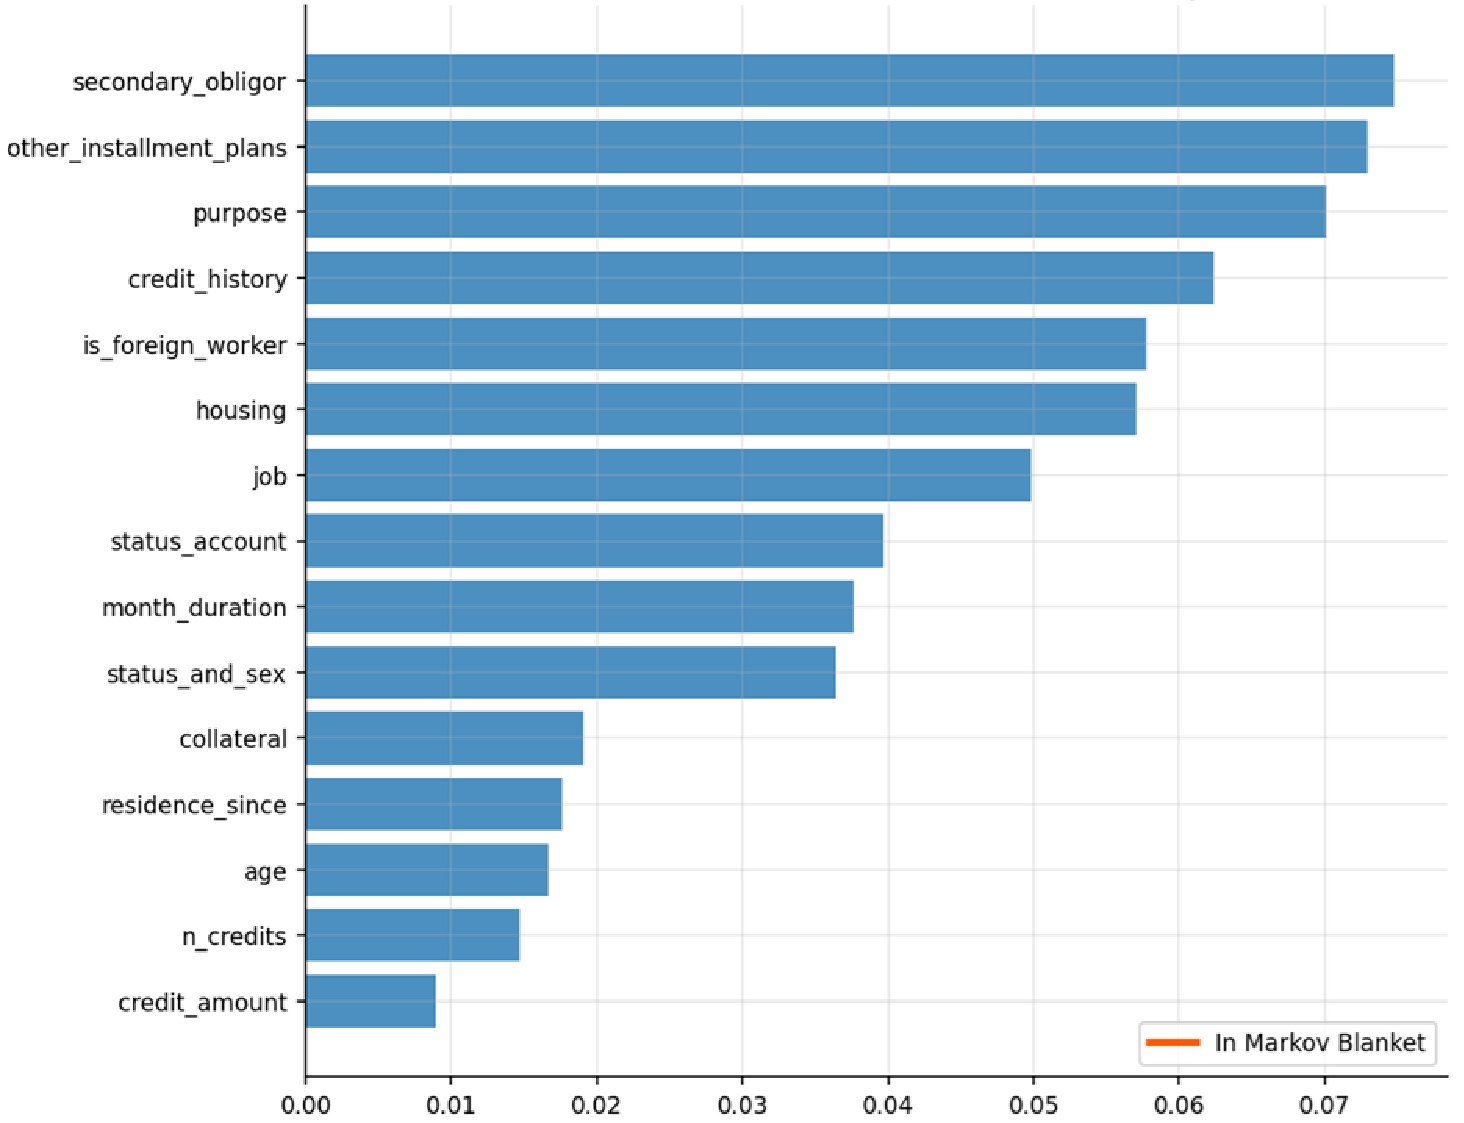
\includegraphics[width=\textwidth]{image/sensitivity/12_sensitivity_ger.pdf}\\[0.1cm]
            {\small Thông tin tương hỗ}
        \end{minipage}    
    \end{subfigure}
    \caption{Biểu đồ độ nhạy ($\delta$) và thông tin tương hỗ trên tập biến thuộc Markov Blanket --- German Credit}
    \label{fig:sens_ger}
\end{figure}

\begin{figure}[H]
    \centering
    \begin{subfigure}[b]{\textwidth}
        \centering
        \begin{minipage}{0.9\textwidth}
            \centering
            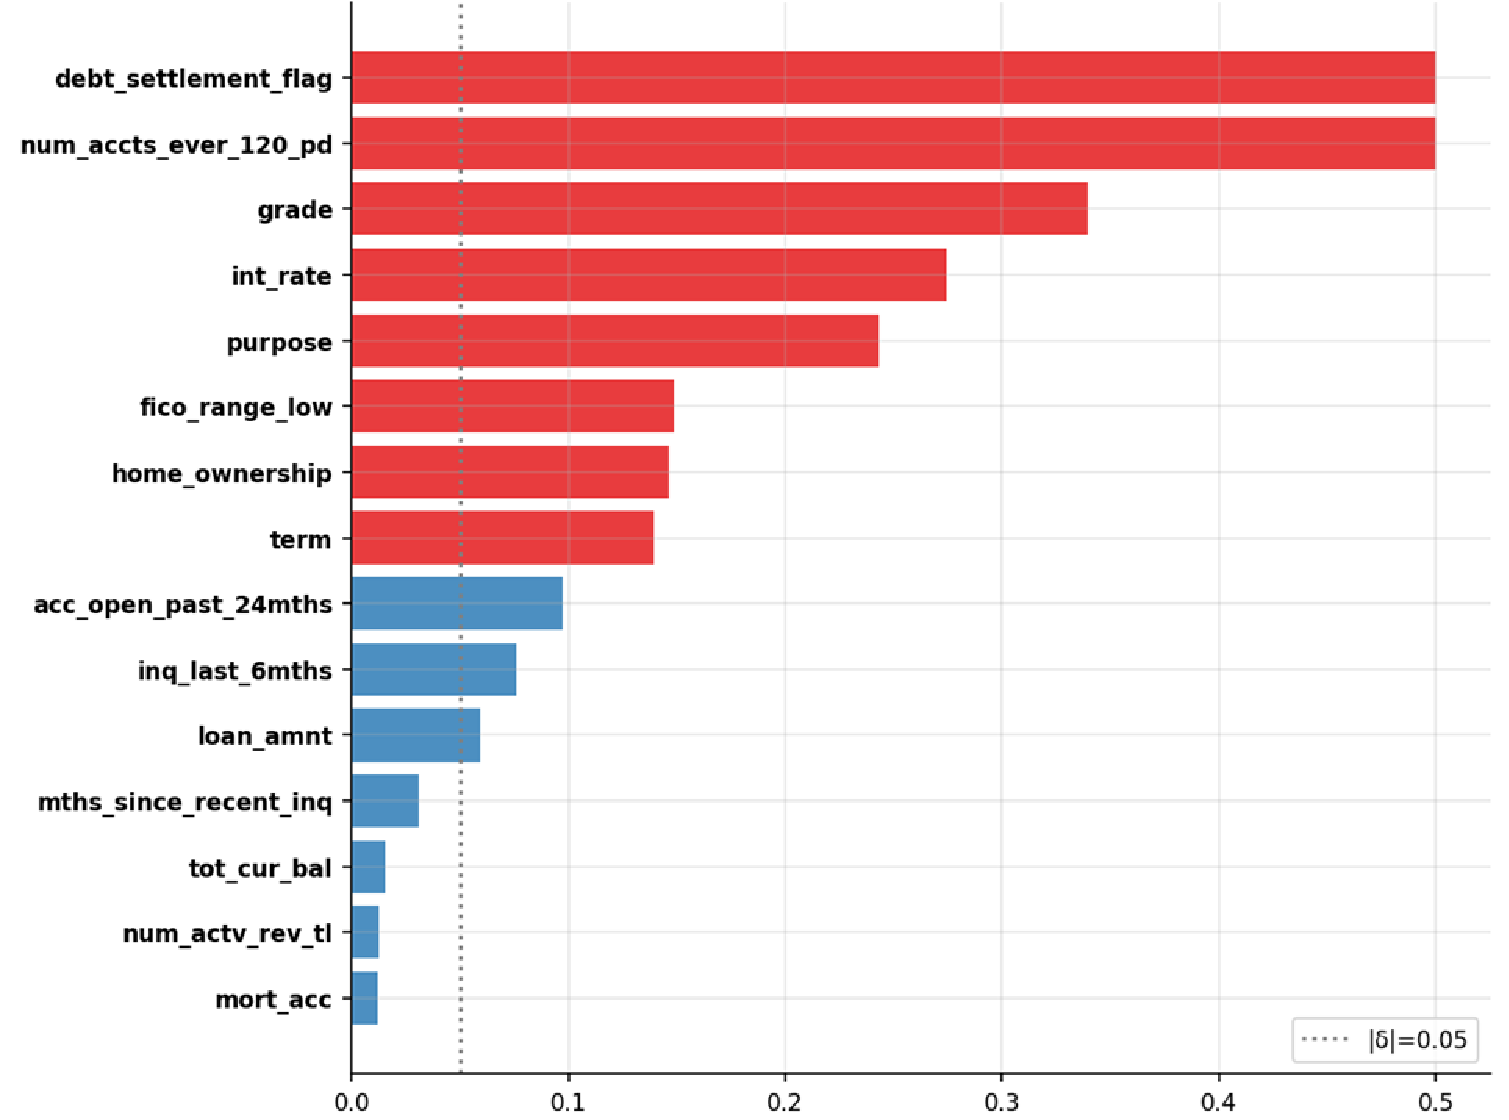
\includegraphics[width=\textwidth]{image/sensitivity/11_sensitivity_lend.pdf}\\[0.1cm]
            {\small Biểu đồ độ nhạy ($\delta$)}
        \end{minipage}
        \vspace{0.3cm}
        \begin{minipage}{0.9\textwidth}
            \centering
            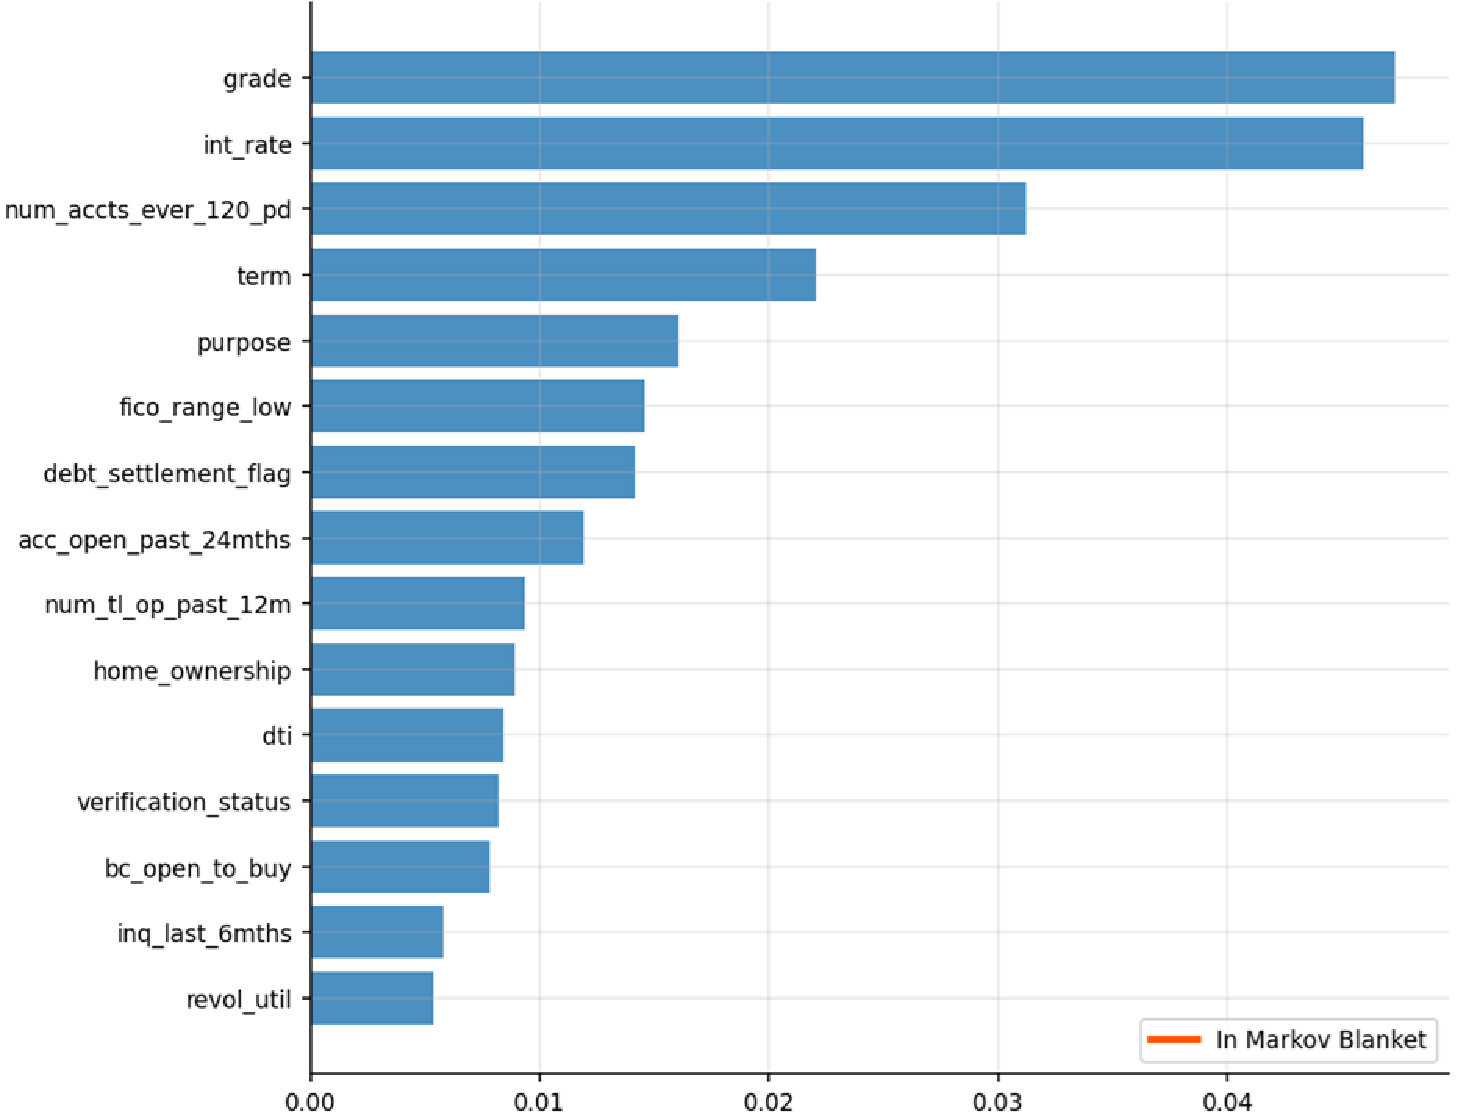
\includegraphics[width=\textwidth]{image/sensitivity/12_sensitivity_lend.pdf}\\[0.1cm]
            {\small Thông tin tương hỗ}
        \end{minipage}    
    \end{subfigure}
    \caption{Biểu đồ độ nhạy ($\delta$) và thông tin tương hỗ trên tập biến thuộc Markov Blanket --- Lending Club}
    \label{fig:sens_lend}
\end{figure}



% =========================================================================
% KHỐI HÌNH 4.8 - PHẦN 1: Australian Credit (lấp khoảng trống còn lại)
% =========================================================================
\begin{figure}[H]
    \centering
    \begin{subfigure}[b]{0.95\textwidth} 
        \centering
        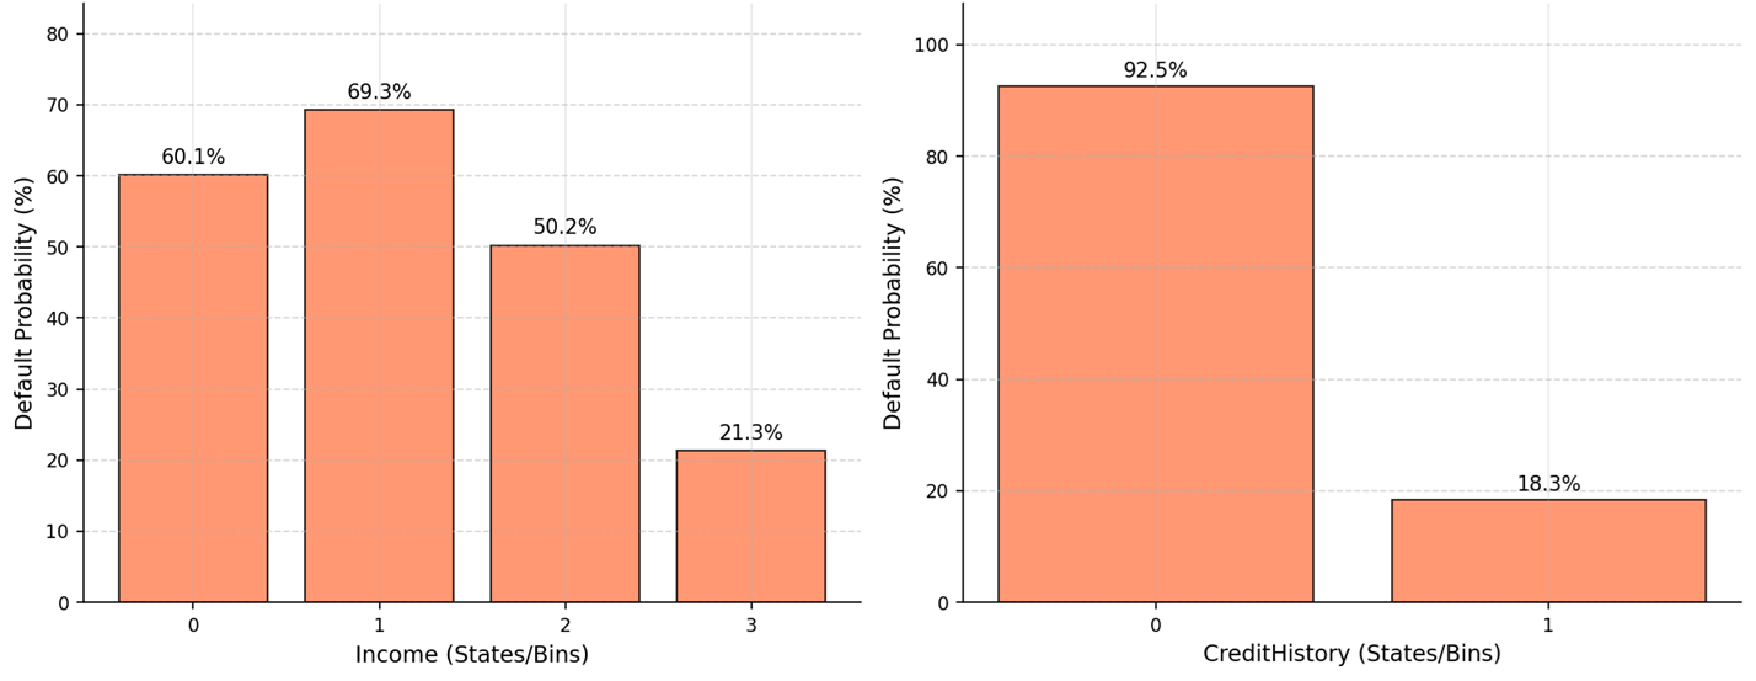
\includegraphics[width=\textwidth]{image/sensitivity/2_sensitivy_au.pdf}       
    \end{subfigure}
    \caption{Xác suất vỡ nợ cận biên khi can thiệp vào các đặc trưng quan trọng --- Australian Credit}
    \label{fig:prob_au}
\end{figure}

\begin{figure}[H]
    \centering
    \begin{subfigure}[b]{0.95\textwidth} 
        \centering
        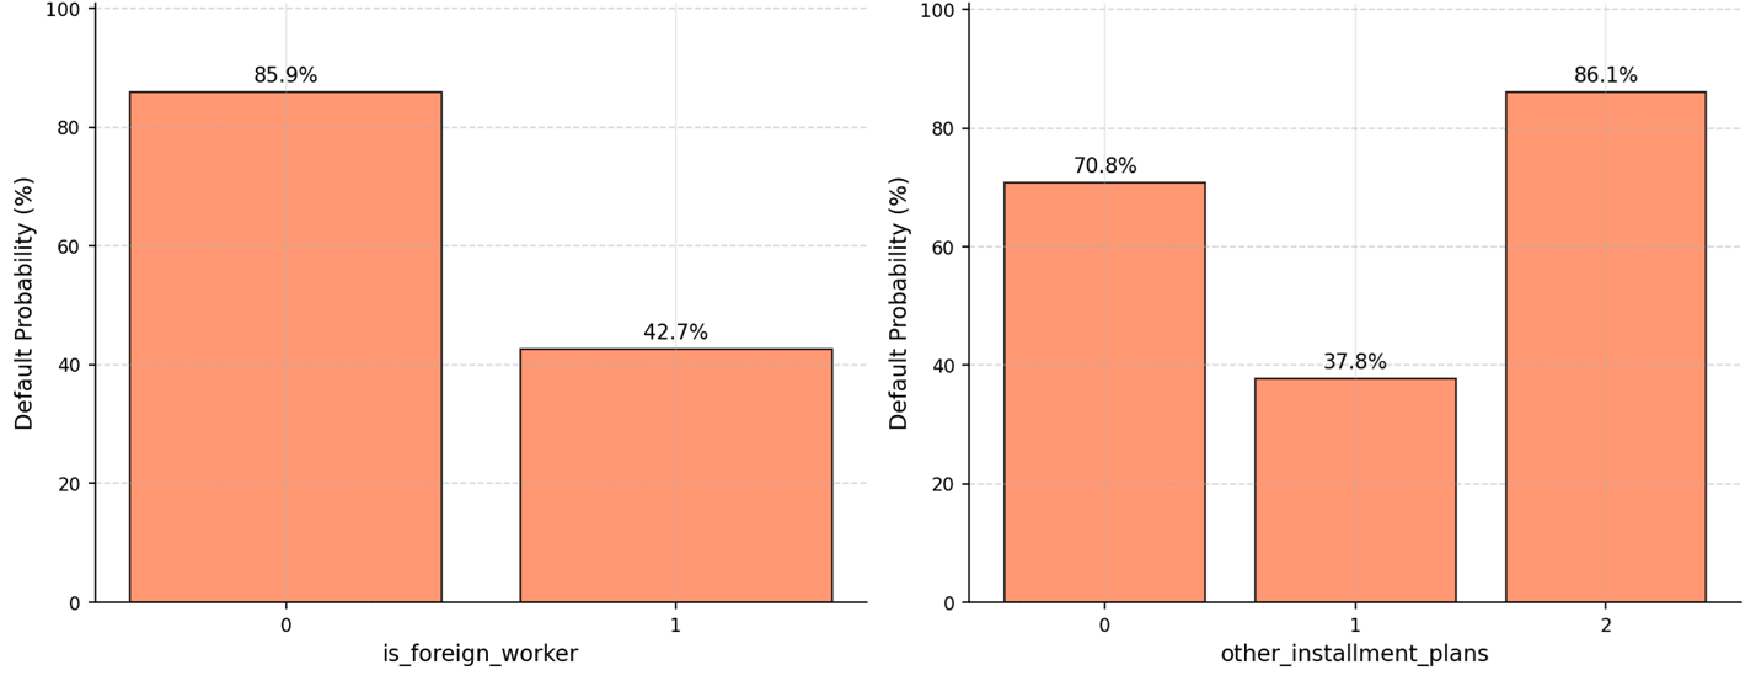
\includegraphics[width=\textwidth]{image/sensitivity/2_sensitivy_ger.pdf}       
    \end{subfigure}
    \caption{Xác suất vỡ nợ cận biên khi can thiệp vào các đặc trưng quan trọng --- German Credit}
    \label{fig:prob_ger}
\end{figure}

\begin{figure}[H]
    \centering
    \begin{subfigure}[b]{1\textwidth} 
        \centering
        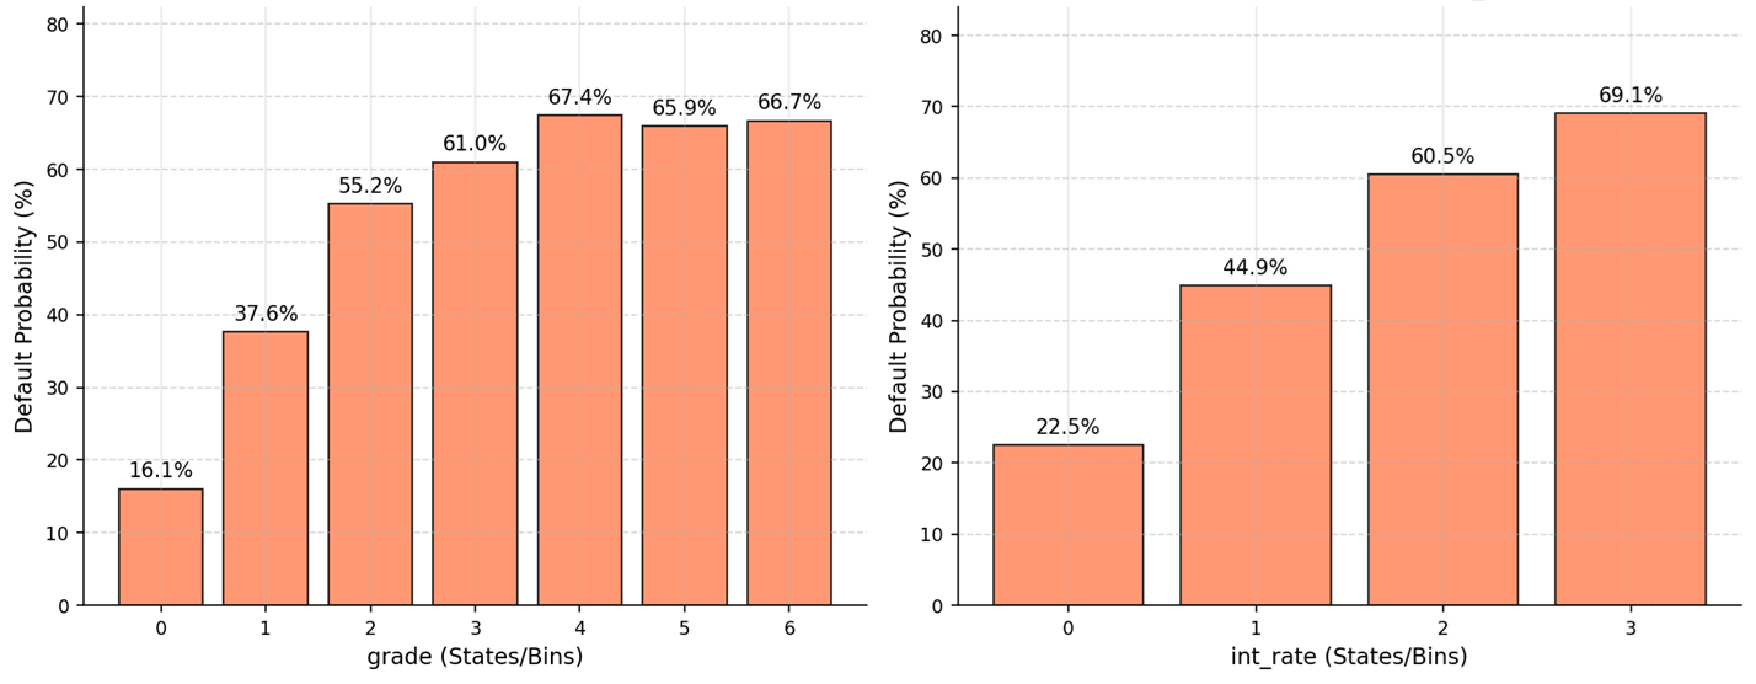
\includegraphics[width=\textwidth]{image/sensitivity/2_sensitivy_lend.pdf}       
    \end{subfigure}
    \caption{Xác suất vỡ nợ cận biên khi can thiệp vào các đặc trưng quan trọng --- Lending Club}
    \label{fig:prob_lend}
\end{figure}

\newpage
\subsubsection{Suy luận tiến}
\label{sec:4.4.2}
\noindent
Suy luận tiến được thực hiện đồng thời trên cặp biến cha (\textit{parent}) trực tiếp của \texttt{target} trong DAG của mỗi bộ dữ liệu, nhằm quan sát hiệu ứng tương tác giữa các nguyên nhân trực tiếp lên xác suất vỡ nợ.

\vspace{1.5em}

% =========================================================================
% KHỐI HÌNH 4.9 - PHẦN 1: Australian Credit (lấp khoảng trống còn lại)
% =========================================================================
\begin{figure}[H]
    \centering
    \begin{subfigure}[b]{0.88\textwidth} 
        \centering
        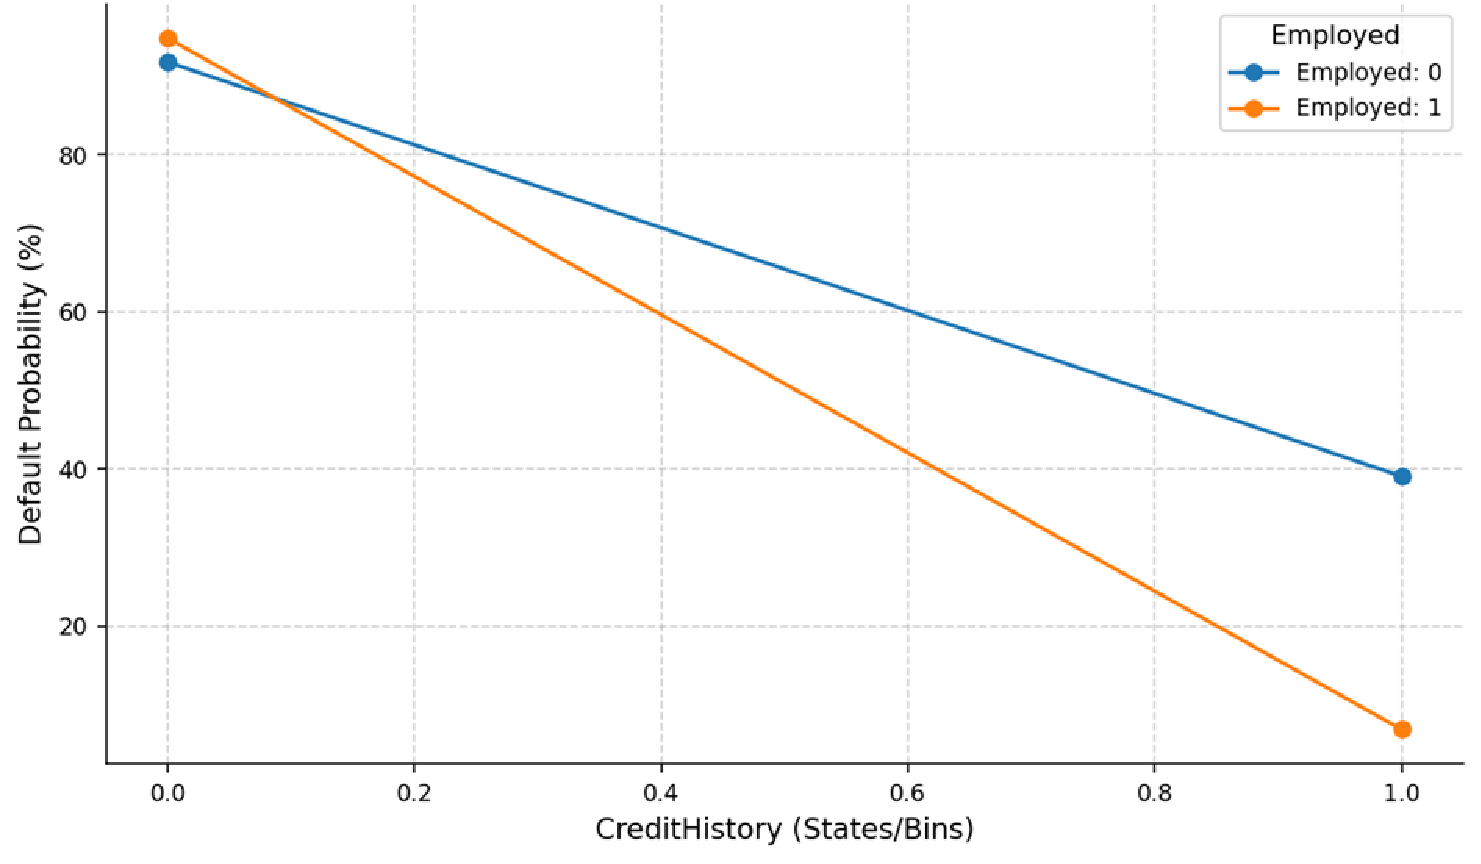
\includegraphics[width=\textwidth]{image/forward/forward_au.pdf}
        \caption{Australian Credit}
        \label{fig:forward_au}
    \end{subfigure}
    
    \vspace{1cm}

    \begin{subfigure}[b]{0.88\textwidth}
        \centering
        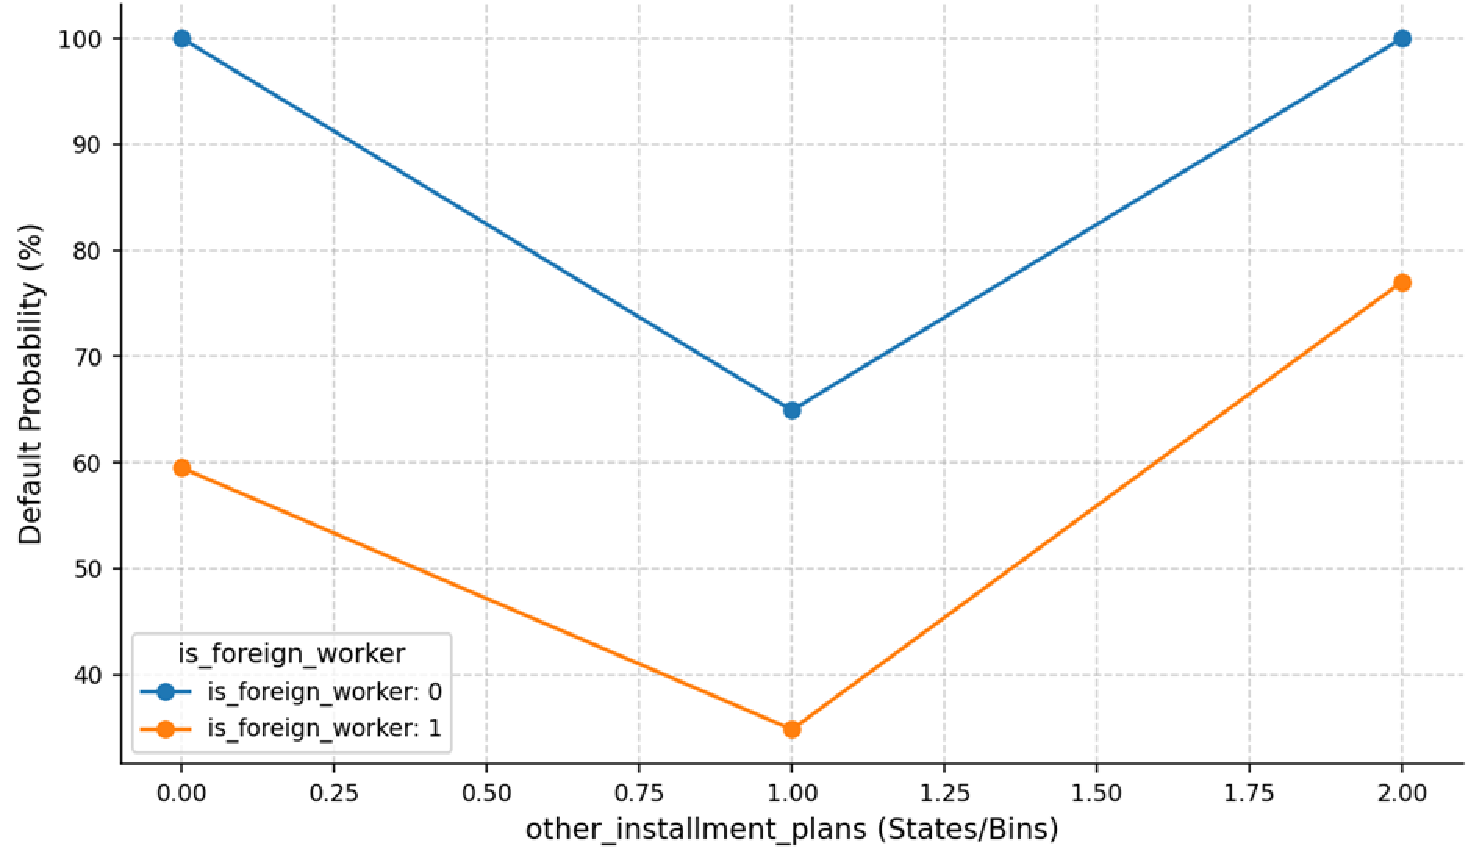
\includegraphics[width=\textwidth]{image/forward/forward_ger.pdf}
        \caption{German Credit}
        \label{fig:forward_ger}
    \end{subfigure}
    
    \caption{Suy luận tiến đồng thời trên cặp biến cha trực tiếp của \texttt{target}}
\end{figure}

% =========================================================================
% KHỐI HÌNH 4.9 - PHẦN 2: German + Lending Club (nối tiếp ngay sau)
% =========================================================================
\begin{figure}[H]
    \ContinuedFloat
    \centering
    
    \begin{subfigure}[b]{0.88\textwidth}
        \centering
        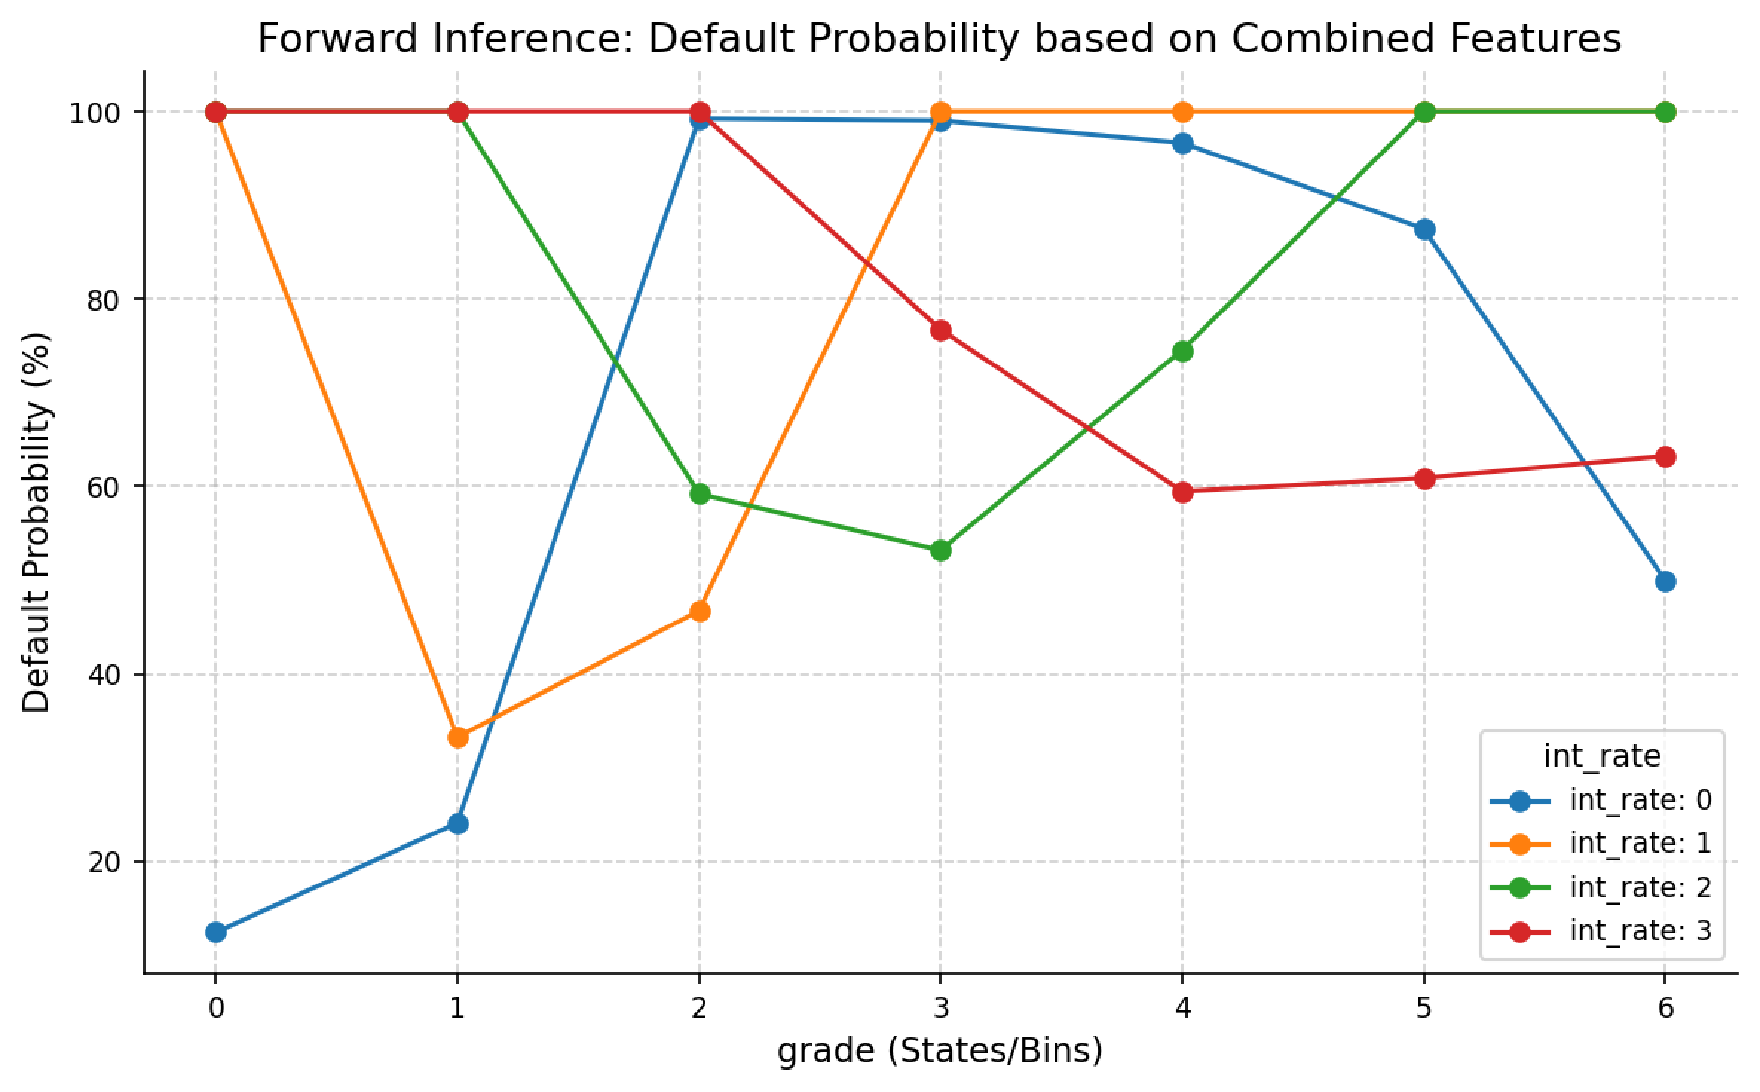
\includegraphics[width=\textwidth]{image/forward/forward_len.pdf}
        \caption{Lending Club}
        \label{fig:forward_len}
    \end{subfigure}
    
    \caption{Suy luận tiến đồng thời trên cặp biến cha trực tiếp của \texttt{target} (tiếp theo)}
    \label{fig:forward_inference}
\end{figure}
\FloatBarrier
Trên Australian Credit, hai biến cha \texttt{CreditHistory} và \texttt{Employed} được gán đồng thời làm bằng chứng. Kết quả tại Hình \ref{fig:forward_au} cho thấy khi khách hàng chưa có lịch sử tín dụng, xác suất vỡ nợ luôn ở mức rất cao bất kể tình trạng việc làm, dao động quanh $93\%$ đối với người chưa có việc làm và tăng nhẹ lên khoảng $95\%$ đối với người đang có việc làm. Khi đã có lịch sử tín dụng, xác suất vỡ nợ giảm mạnh ở cả hai nhóm, nhưng mức giảm rõ rệt hơn hẳn ở nhóm đang có việc làm, chỉ còn khoảng $7\%$, so với khoảng $39\%$ ở nhóm chưa có việc làm. Nói cách khác, \texttt{Employed} không thể hiện vai trò bảo vệ đáng kể khi \texttt{CreditHistory} ở trạng thái bất lợi, nhưng lại khuếch đại rõ rệt hiệu ứng tích cực của \texttt{CreditHistory} khi biến này ở trạng thái thuận lợi.

Trên German Credit, hai biến cha \texttt{is\_foreign\_worker} và \texttt{other\_installment\_plans} được khảo sát đồng thời. Hình \ref{fig:forward_ger} cho thấy cả hai đường ứng với \texttt{is\_foreign\_worker} đều giữ nguyên hình dạng chữ V đã ghi nhận ở \ref{sec:4.4.1} đối với \texttt{other\_installment\_plans}, nhưng bị dịch chuyển theo hai biên độ khác nhau: nhóm lao động nước ngoài đạt xác suất vỡ nợ tối đa $100\%$ ở cả hai trạng thái ``Bank'' và ``none'', trong khi nhóm không phải lao động nước ngoài dù cùng biểu hiện chữ V nhưng đáy và đỉnh đều thấp hơn đáng kể, chỉ dao động trong khoảng $35\%$--$77\%$. Kết quả này cho thấy \texttt{is\_foreign\_worker} đóng vai trò như một biến khuếch đại làm trầm trọng thêm hiệu ứng phi tuyến vốn đã tồn tại của \texttt{other\_installment\_plans}.

Trên Lending Club, hai biến cha \texttt{grade} và \texttt{int\_rate} được khảo sát đồng thời. Khác hẳn với hai bộ dữ liệu trên, Hình \ref{fig:forward_len} cho thấy quan hệ giữa hai biến này không còn đơn điệu hay có quy luật rõ ràng, mà dao động thất thường: ở \texttt{grade} thấp nhất (hạng A, state 0), xác suất vỡ nợ chỉ đạt $13\%$ ở \texttt{int\_rate} thấp nhất nhưng lại nhảy vọt lên gần $100\%$ ở cả ba mức \texttt{int\_rate} còn lại; trong khi đó, ở \texttt{grade} cao nhất (hạng G, state 6), xu hướng gần như đảo ngược khi \texttt{int\_rate} thấp nhất lại cho xác suất vỡ nợ cao nhất trong nhóm ($50\%$) còn ba mức \texttt{int\_rate} còn lại đều xấp xỉ $60\%$--$100\%$. Hiện tượng dao động phi quy luật này nhiều khả năng bắt nguồn từ mối tương quan rất cao giữa \texttt{grade} và \texttt{int\_rate} trong thực tế cho vay của Lending Club, vốn dĩ lãi suất được ấn định phần lớn dựa trên hạng tín dụng ngay từ khâu thẩm định; hệ quả là nhiều tổ hợp (\texttt{grade}, \texttt{int\_rate}) hiếm gặp hoặc gần như không tồn tại trong tập huấn luyện, khiến bảng CPT tương ứng được ước lượng trên rất ít quan sát và cho ra xác suất cực trị kém ổn định, tương tự hiện tượng dữ liệu thưa đã ghi nhận ở Mục \ref{sec:4.4.1} đối với \texttt{debt\_settlement\_flag} và \texttt{num\_accts\_ever\_120\_pd}. Kết quả này là một minh chứng rõ ràng cho giới hạn của việc suy luận đồng thời trên hai biến có tương quan nội tại cao, và cần được diễn giải hết sức thận trọng thay vì rút ra kết luận nhân quả trực tiếp.

Nhìn chung, suy luận tiến trên cặp biến cha đồng thời cho thấy mức độ tương tác giữa các đặc trưng không đồng nhất: Australian Credit và German Credit thể hiện tương tác khuếch đại có quy luật rõ ràng, trong khi Lending Club lại bộc lộ giới hạn của phương pháp khi hai biến cha được chọn có tương quan nội tại quá cao, dẫn đến hiện tượng dữ liệu thưa trong không gian tổ hợp. Phát hiện này khẳng định giá trị bổ sung của suy luận tiến đa biến so với phân tích độ nhạy đơn biến, đồng thời cũng cho thấy việc lựa chọn cặp biến cha để suy luận đồng thời cần cân nhắc thêm yếu tố tương quan nội tại giữa chúng, chứ không chỉ dựa vào quan hệ nhân quả trực tiếp với \texttt{target}.

\subsubsection{Suy luận lùi}
\noindent
Suy luận lùi được thực hiện trên từng biến cha trực tiếp của \texttt{target} trong DAG của mỗi bộ dữ liệu, truy vấn $P(X_i \mid \text{target}=1)$ so với $P(X_i \mid \text{target}=0)$ nhằm truy vết đặc điểm chung của nhóm hồ sơ đã vỡ nợ so với nhóm không vỡ nợ.

Trên Australian Credit, \texttt{CreditHistory} và \texttt{Employed} là hai biến cha được truy vấn. Kết quả tại Hình \ref{fig:backward_au} cho thấy trong nhóm khách hàng đã vỡ nợ, $79.1\%$ không có lịch sử tín dụng, trong khi tỷ lệ này ở nhóm không vỡ nợ chỉ là $6.5\%$, mức chênh lệch lớn nhất trong toàn bộ kết quả \textit{backward inference} của cả ba bộ dữ liệu, khẳng định \texttt{CreditHistory} là dấu hiệu chẩn đoán mạnh nhất để truy vết một hồ sơ đã vỡ nợ. Tương tự, $77.4\%$ nhóm vỡ nợ chưa có việc làm tại thời điểm nộp đơn, so với $30.3\%$ ở nhóm không vỡ nợ, thấp hơn đáng kể so với chênh lệch của \texttt{CreditHistory} nhưng vẫn thể hiện khả năng phân biệt rõ ràng.

Trên German Credit, \texttt{is\_foreign\_worker} và \texttt{other\_installment\_plans} là hai biến cha được truy vấn tại Hình \ref{fig:backward_ger}. Đối với \texttt{is\_foreign\_worker}, $29.19\%$ nhóm vỡ nợ là lao động nước ngoài so với chỉ $4.78\%$ ở nhóm không vỡ nợ, mức chênh lệch cao thứ nhì trong toàn bộ kết quả \textit{backward inference} của ba bộ dữ liệu, chỉ sau \texttt{CreditHistory} của Australian Credit. Đối với \texttt{other\_installment\_plans}, trạng thái ``none'' chiếm $20.81\%$ trong nhóm vỡ nợ so với chỉ $3.35\%$ ở nhóm không vỡ nợ, trong khi trạng thái ``stores'' lại phổ biến hơn hẳn ở nhóm không vỡ nợ ($85.41\%$) so với nhóm vỡ nợ ($51.91\%$). Kết quả này cho thấy chiều phân biệt của \texttt{other\_installment\_plans} không tập trung ở một trạng thái duy nhất mà trải đều ở hai đầu ``Bank'' và ``none'', nhất quán với hình dạng chữ V phi tuyến đã ghi nhận ở Mục \ref{sec:4.4.1} và \ref{sec:4.4.2}.


% =========================================================================
% KHỐI HÌNH 4.10 - PHẦN 1: Australian Credit (lấp khoảng trống còn lại)
% =========================================================================
\begin{figure}[H]
    \centering
    \begin{subfigure}[b]{\textwidth}
        \centering
        \begin{minipage}{0.49\textwidth}
            \centering
            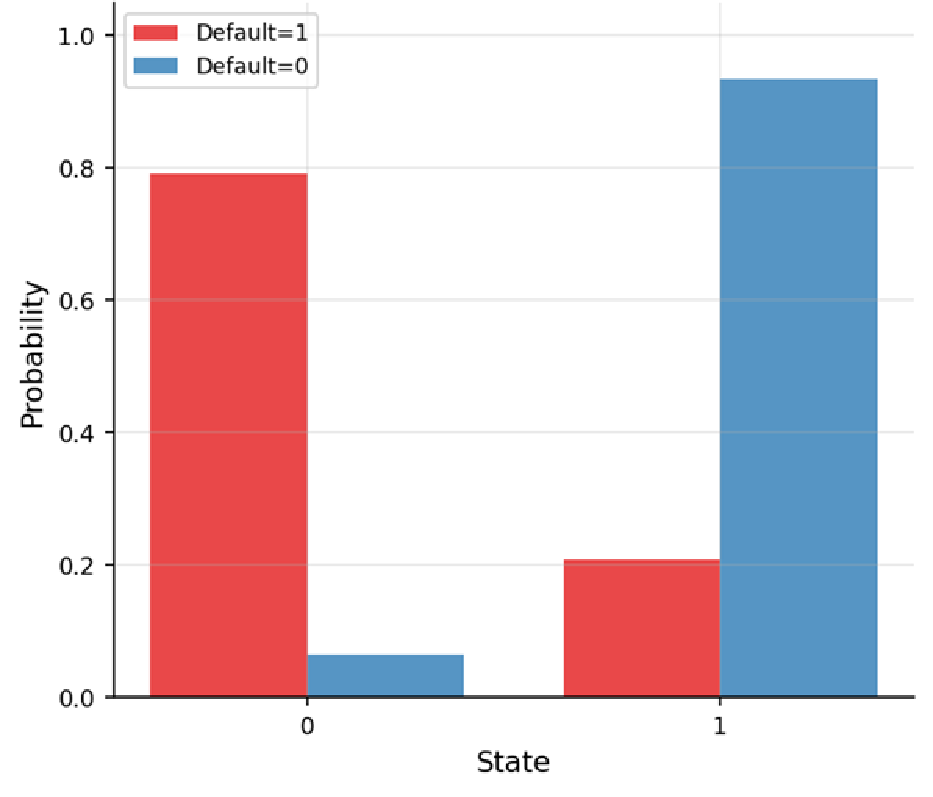
\includegraphics[width=\textwidth]{image/backward/backward_au_crehis.pdf}\\[0.1cm]
            \caption{\texttt{CreditHistory}}
        \end{minipage}
        \hfill
        \begin{minipage}{0.49\textwidth}
            \centering
            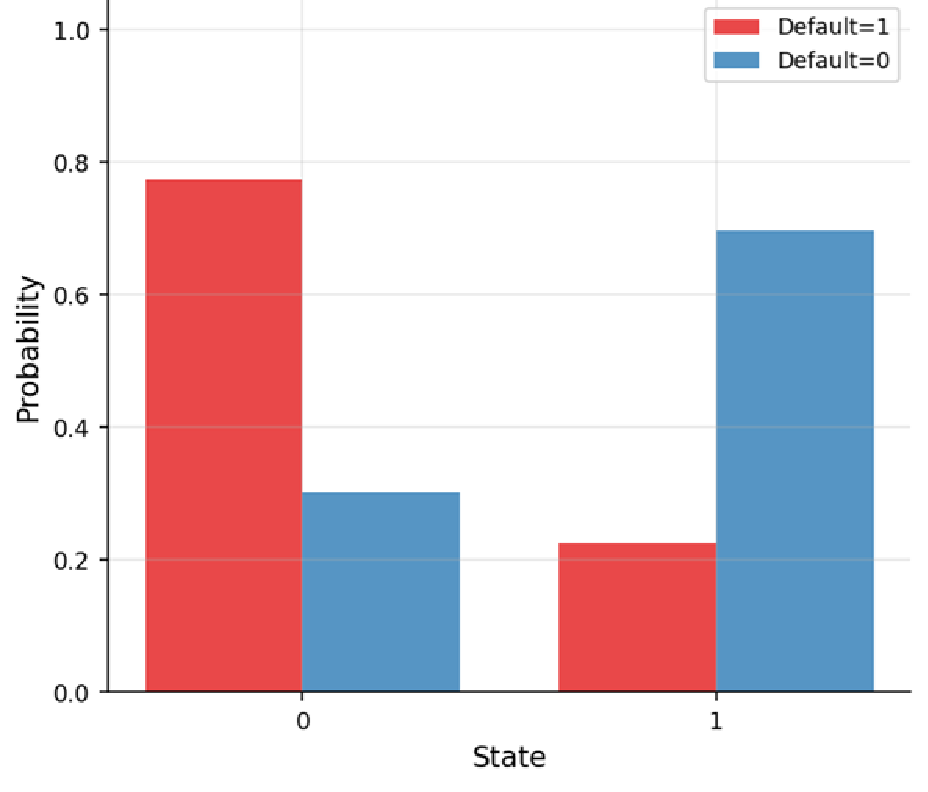
\includegraphics[width=\textwidth]{image/backward/backward_au_employ.pdf}\\[0.1cm]
            \caption{\texttt{Employed}}
        \end{minipage}
    \end{subfigure}
    \caption{Suy luận lùi trên các biến cha trực tiếp của \texttt{target} --- Australian Credit}
    \label{fig:backward_au}
\end{figure}

\begin{figure}[H]
    \centering
    \begin{subfigure}[b]{\textwidth}
        \centering
        \begin{minipage}{0.49\textwidth}
            \centering
            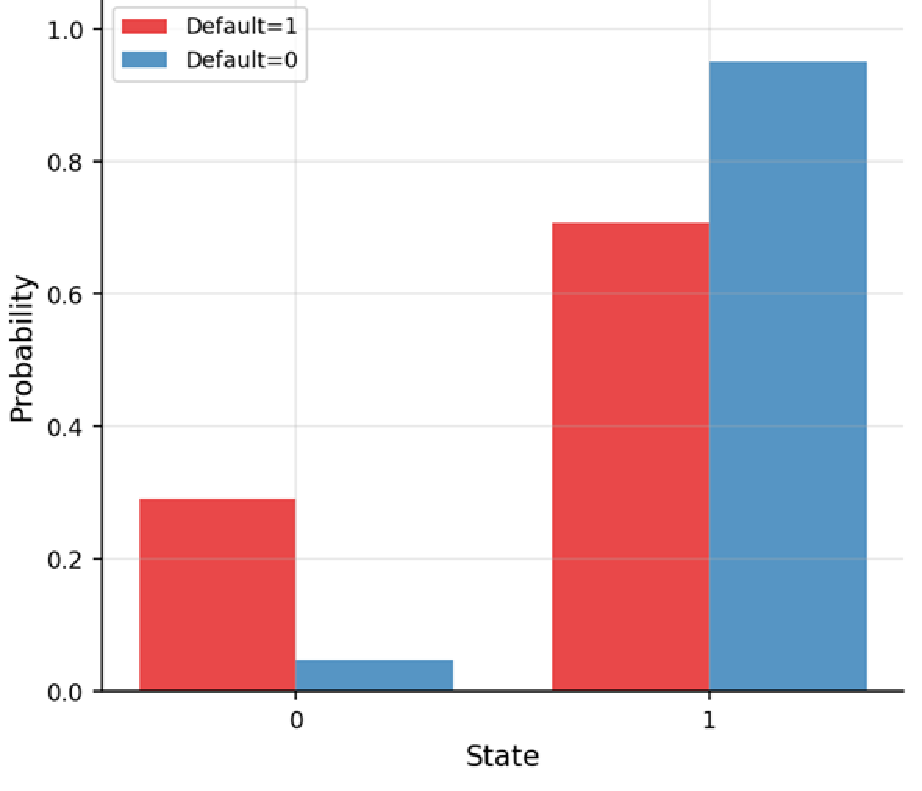
\includegraphics[width=\textwidth]{image/backward/backward_ger_foreign.pdf}\\[0.1cm]
            \caption{\texttt{is\_foreign\_worker}}
        \end{minipage}
        \hfill
        \begin{minipage}{0.49\textwidth}
            \centering
            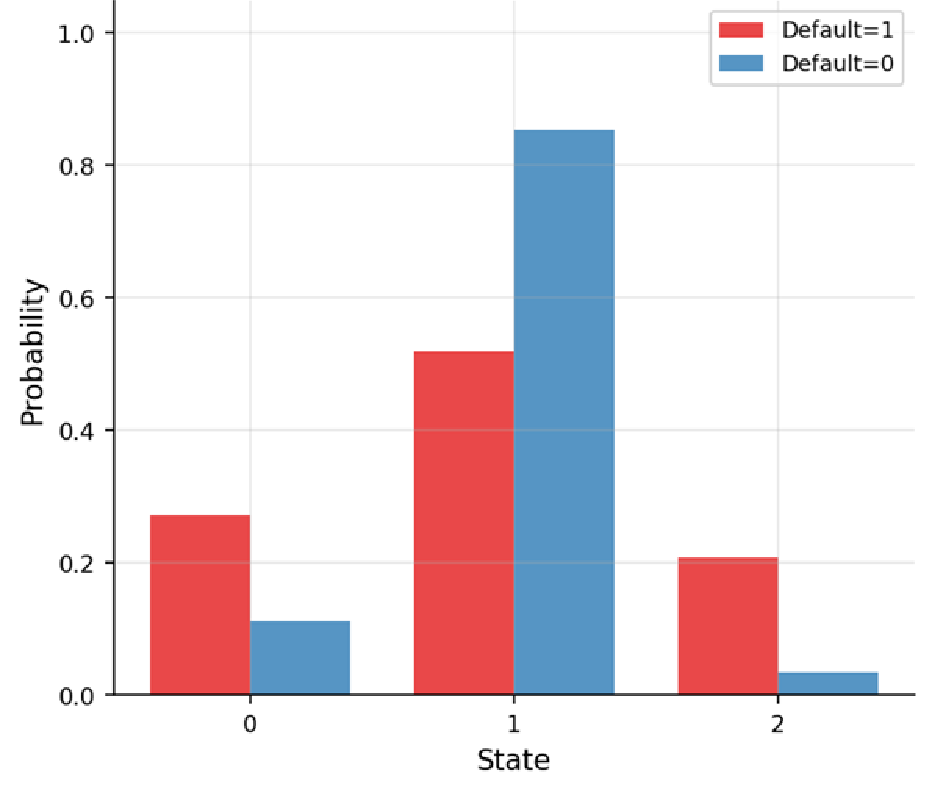
\includegraphics[width=\textwidth]{image/backward/backward_ger_otherins.pdf}\\[0.1cm]
            \caption{\texttt{other\_installment\_plans}}
        \end{minipage}
    \end{subfigure}
    \caption{Suy luận lùi trên các biến cha trực tiếp của \texttt{target} --- German Credit}
    \label{fig:backward_ger}
\end{figure}

Trên Lending Club, \texttt{int\_rate} và \texttt{grade} là hai biến cha được truy vấn ở Hình \ref{fig:backward_lend}. Đối với \texttt{int\_rate}, \textit{bin} lãi suất cao nhất chiếm $20.13\%$ trong nhóm vỡ nợ so với chỉ $9.01\%$ ở nhóm không vỡ nợ, trong khi \textit{bin} lãi suất thấp nhất lại phổ biến hơn hẳn ở nhóm không vỡ nợ ($25.05\%$) so với nhóm vỡ nợ ($7.29\%$), nhất quán với chiều tác động thuận đã ghi nhận ở Mục \ref{sec:4.4.1} và \ref{sec:4.4.2}. Đối với \texttt{grade}, tỷ trọng trong nhóm vỡ nợ tăng dần đều theo hạng tín dụng xấu dần, từ $3.08\%$ ở hạng A lên đến $33.47\%$ ở hạng C trước khi giảm dần ở các hạng thấp hơn do quy mô mẫu nhỏ, trong khi tỷ trọng ở nhóm không vỡ nợ lại tập trung nhiều nhất ở hạng B ($31.04\%$) và giảm dần về sau cho thấy phân phối \texttt{grade} của nhóm vỡ nợ lệch rõ rệt về phía các hạng tín dụng kém hơn so với nhóm không vỡ nợ.

\begin{figure}[H]
    \centering
    \begin{subfigure}[b]{\textwidth}
        \centering
        \begin{minipage}{0.49\textwidth}
            \centering
            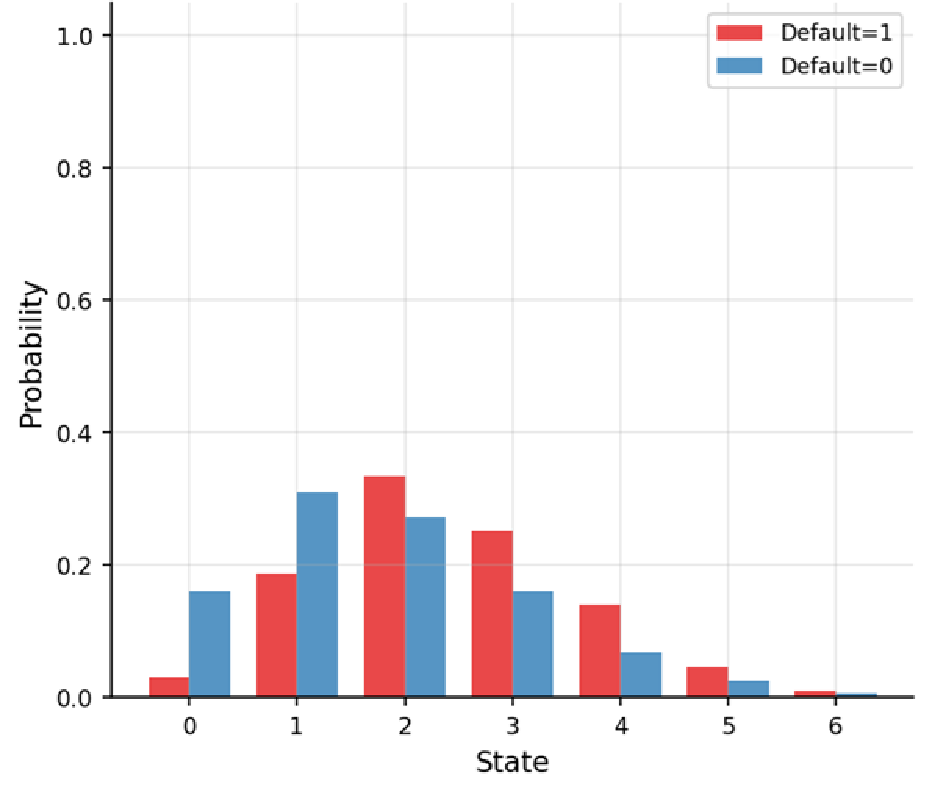
\includegraphics[width=\textwidth]{image/backward/backward_lend_grade.pdf}\\[0.1cm]
            \caption{\texttt{grade}}
        \end{minipage}
        \hfill
        \begin{minipage}{0.49\textwidth}
            \centering
            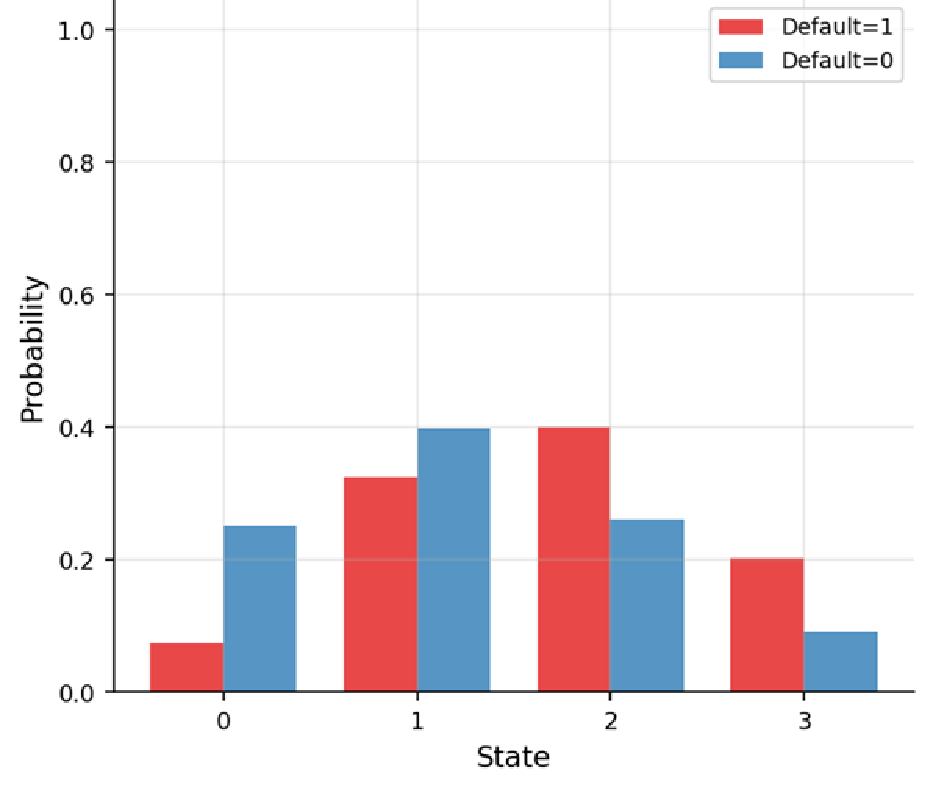
\includegraphics[width=\textwidth]{image/backward/backward_lend_int.pdf}\\[0.1cm]
            \caption{\texttt{int\_rate}}
        \end{minipage}
    \end{subfigure}
    \caption{Suy luận lùi trên các biến cha trực tiếp của \texttt{target} --- Lending Club}
    \label{fig:backward_lend}
\end{figure}
Để có cái nhìn toàn cục hơn thay vì chỉ giới hạn ở các biến cha, suy luận lùi còn được mở rộng ra toàn bộ các nút của mạng: gán \texttt{target}=0 và \texttt{target}=1 lần lượt làm evidence, sau đó truy vấn lại phân phối hậu nghiệm của mọi biến còn lại, thể hiện tại Hình \ref{fig:backward_australian}, \ref{fig:backward_german} và  \ref{fig:backward_lendingclub} mỗi hình gồm hai đồ thị ứng với \texttt{target} = 0 và \texttt{target} = 1.

\begin{figure}[H]
    \centering
    \begin{subfigure}[b]{\textwidth}
        \centering
        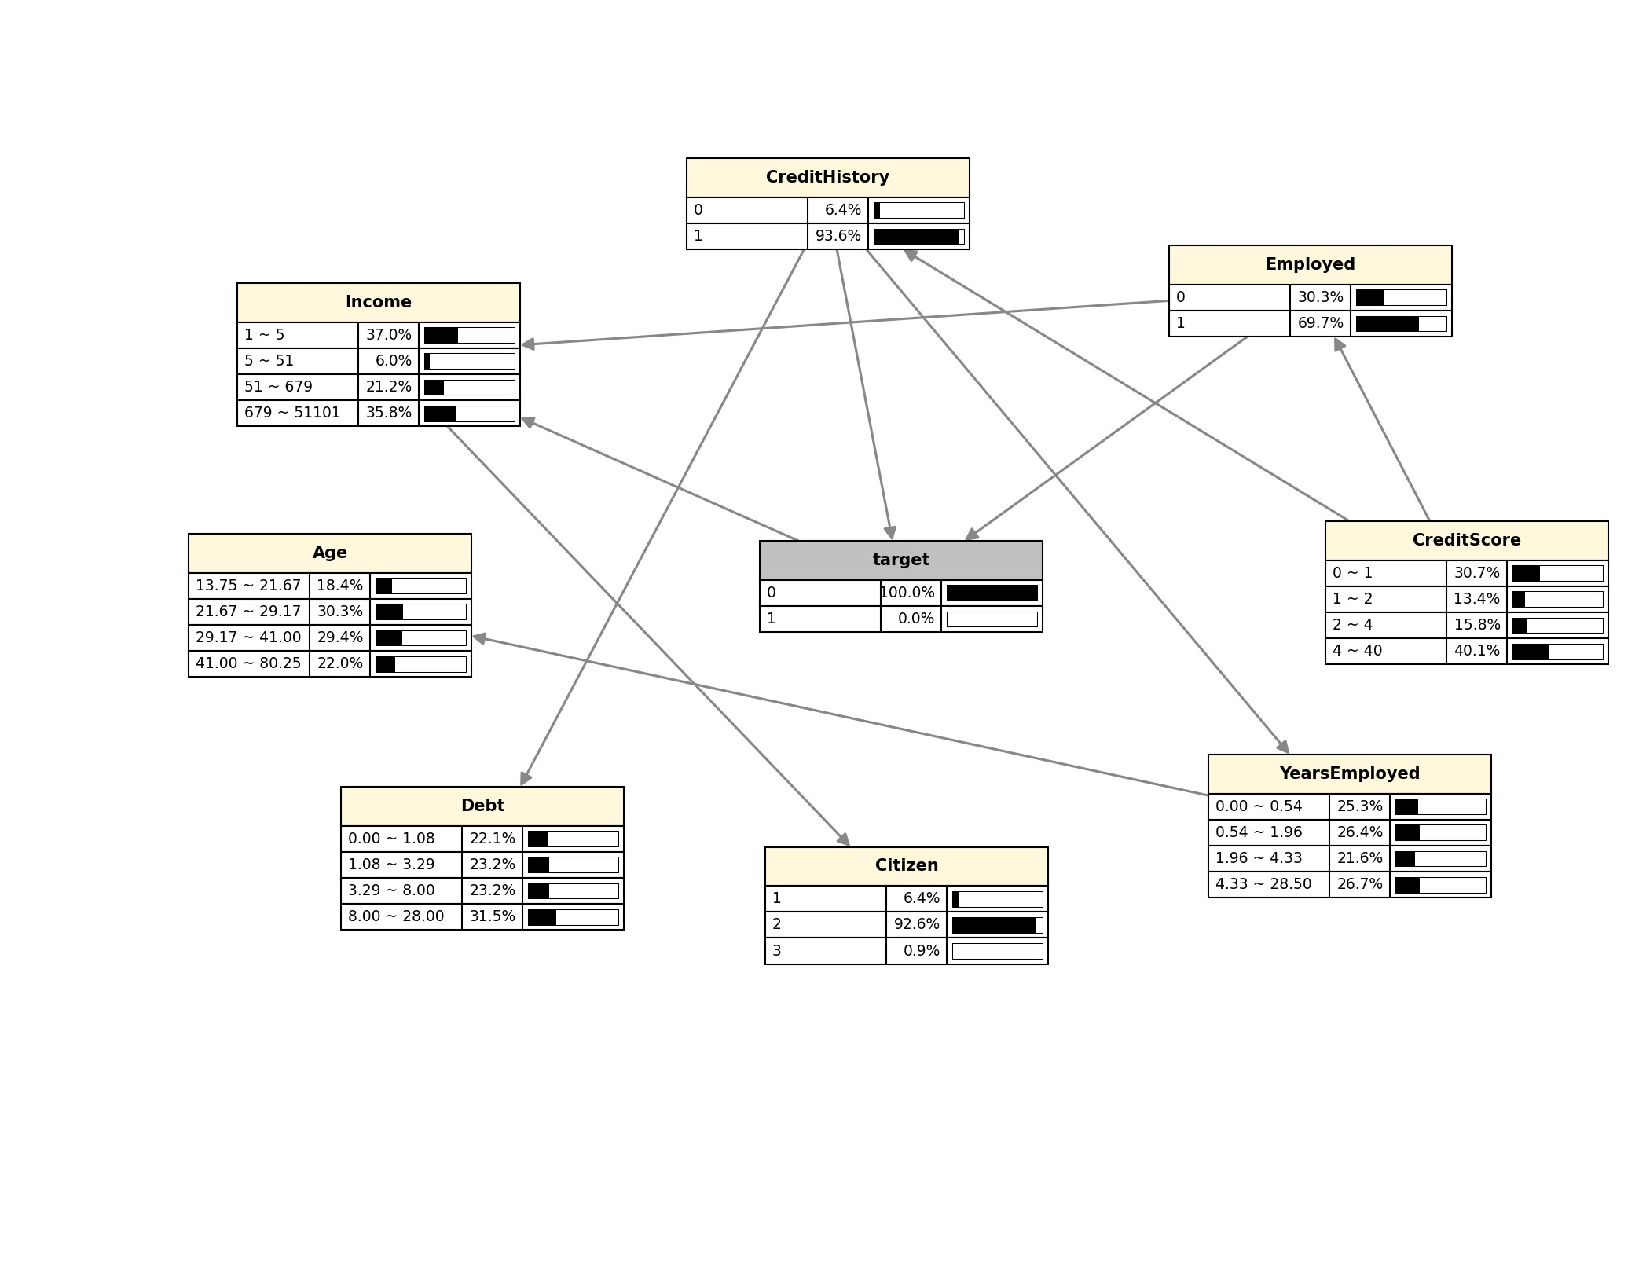
\includegraphics[width=1.05\textwidth,
        height=0.43\textheight,
        trim=3cm 5cm 0cm 2.5cm,
        clip
        ]{image/backward/au_back_0.pdf}
        \caption{target = 0}
        \label{fig:au_back_0}
    \end{subfigure}
    \caption{Suy luận lùi toàn cục theo evidence target --- Australian Credit}
\end{figure}
    
\begin{figure}
    \ContinuedFloat
    \centering
    \begin{subfigure}[b]{\textwidth}
        \centering
        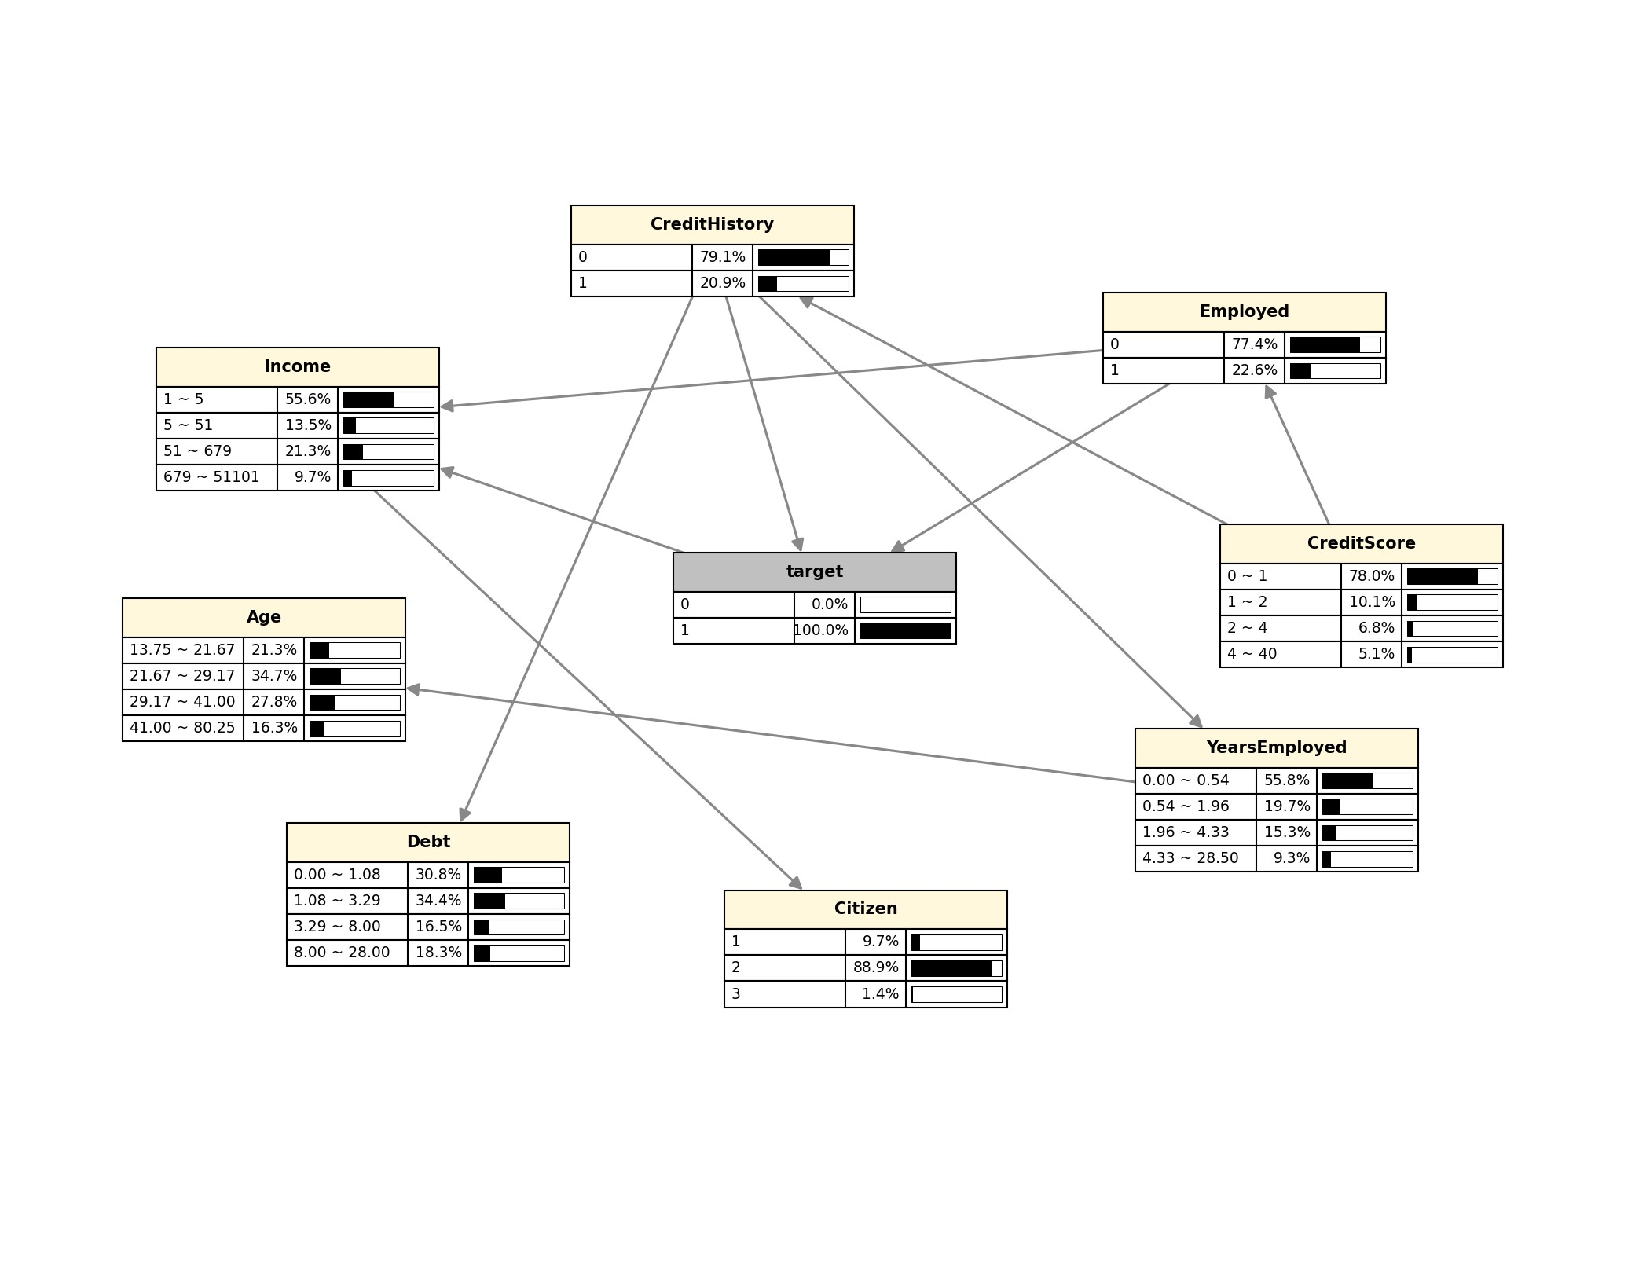
\includegraphics[width=1.1\textwidth,
        height=0.5\textheight,
        trim=2cm 4cm 0cm 3cm,
        clip]{image/backward/au_back_1.pdf}
        \caption{target = 1}
        \label{fig:au_back_1}
    \end{subfigure}
    \caption{Suy luận lùi toàn cục theo evidence target --- Australian Credit (tiếp theo)}
    \label{fig:backward_australian}
\end{figure}


Trên Australian Credit, \texttt{CreditHistory} dịch chuyển mạnh nhất trong toàn mạng (Hình \ref{fig:backward_australian}): từ tiên nghiệm 42.9\%/57.1\% (không/có lịch sử) lệch hẳn về 79.1\%/20.9\% khi \texttt{target}=1 và ngược lại về 6.4\%/93.6\% khi \texttt{target}=0. \texttt{Employed} cũng dịch chuyển đáng kể (53.9\%/46.1\% tiên nghiệm $\rightarrow$ 77.4\%/22.6\% khi vỡ nợ $\rightarrow$ 30.3\%/69.7\% khi không vỡ nợ), trong khi \texttt{Citizen} hầu như không đổi qua cả ba kịch bản (dao động trong khoảng 1 điểm phần trăm), củng cố nhận định rằng đây là biến ít liên quan đến rủi ro tín dụng dù vẫn nằm trong tập đặc trưng được chọn.


Trên German Credit, ba biến dịch chuyển rõ rệt nhất (Hình \ref{fig:backward_german}) là \texttt{credit\_history}, \texttt{other\_installment\_plans} và \texttt{secondary\_obligor}. Đáng chú ý nhất là \texttt{secondary\_obligor}: trạng thái "guarantor" (có người bảo lãnh) chiếm 73.2\% ở phân phối tiên nghiệm, tăng lên 89.7\% ở nhóm không vỡ nợ nhưng giảm còn 56.7\% ở nhóm vỡ nợ cho thấy sự hiện diện của người bảo lãnh có vai trò bảo vệ rõ rệt trên quy mô toàn mạng chứ không chỉ trong quan hệ trực tiếp với \texttt{is\_foreign\_worker} đã phân tích trước đó. Tương tự, \texttt{other\_installment\_plans} lệch từ 68.7\% (trạng thái "stores" ở tiên nghiệm) lên 85.4\% ở nhóm không vỡ nợ nhưng chỉ còn 51.9\% ở nhóm vỡ nợ.

Trên Lending Club, dịch chuyển đáng chú ý nhất và mang tính chẩn đoán cao nhất toàn mạng (Hình \ref{fig:backward_lendingclub}) là \texttt{debt\_settlement\_flag}: ở nhóm không vỡ nợ, biến này đạt 100\% tại trạng thái "không" tức trong dữ liệu, không có bất kỳ khách hàng không vỡ nợ nào từng tham gia chương trình tái cơ cấu nợ trong khi ở nhóm vỡ nợ tỷ lệ "có" tăng lên 4.0\% so với 2.0\% ở tiên nghiệm. \texttt{grade} và \texttt{int\_rate} cũng dịch chuyển nhất quán với các phân tích trước: nhóm vỡ nợ lệch hẳn về các hạng thấp và lãi suất cao (ví dụ hạng G tăng từ 0.8\% tiên nghiệm lên 1.0\%, trong khi hạng A giảm từ 9.6\% xuống 3.1\%), còn nhóm không vỡ nợ lệch ngược lại về phía hạng A và lãi suất thấp (hạng A tăng lên 16.1\%, bin lãi suất thấp nhất tăng lên 25.0\%).

\begin{figure}[H]
    \centering
    \begin{subfigure}[b]{\textwidth}
        \centering
        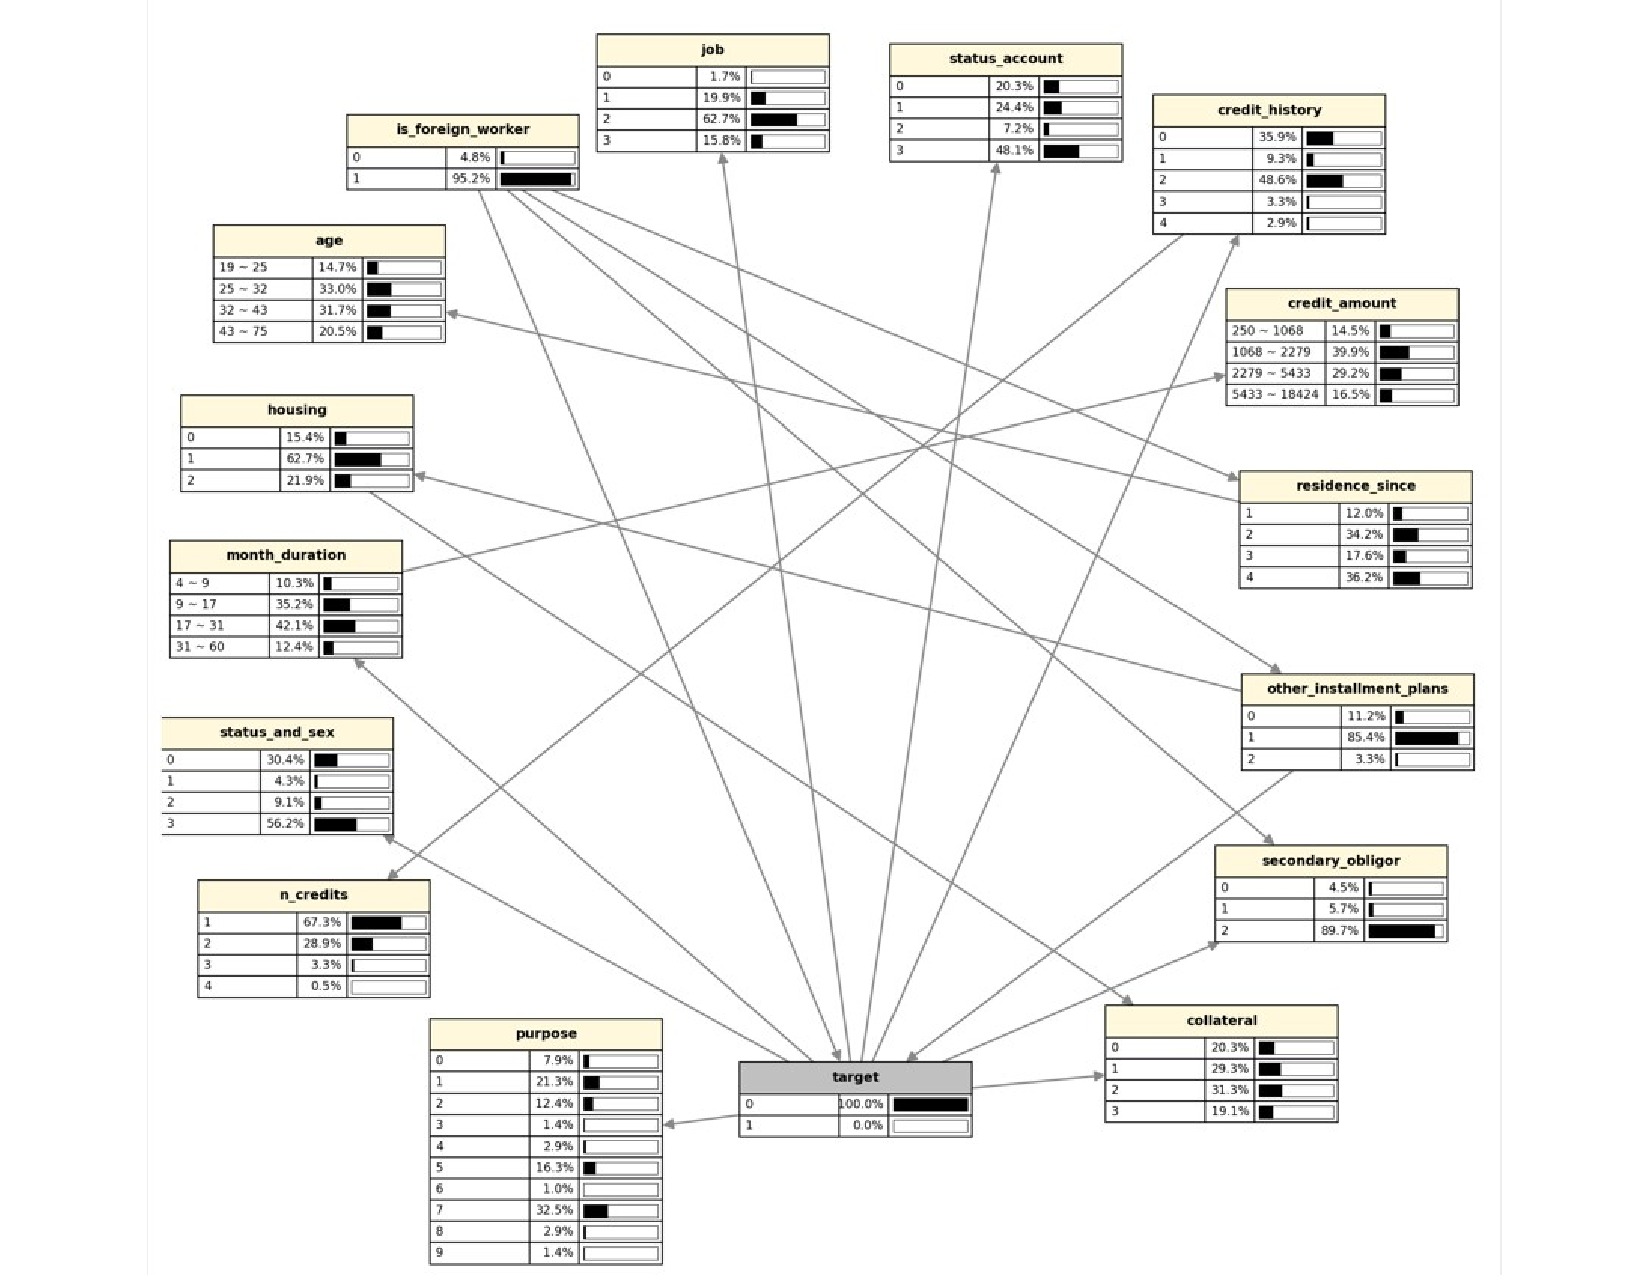
\includegraphics[width=1.2\textwidth,
        height=0.7\textheight,
        trim=1.5cm 0cm 0cm 0.5cm,
        clip]{image/backward/ger_back_0.pdf}
        \caption{target = 0}
        \label{fig:ger_back_0}
    \end{subfigure}
    \caption{Suy luận lùi toàn cục theo evidence target --- German Credit}
\end{figure}

 \begin{figure}[H]
    \ContinuedFloat
    \centering   
    \begin{subfigure}[b]{\textwidth}
        \centering
        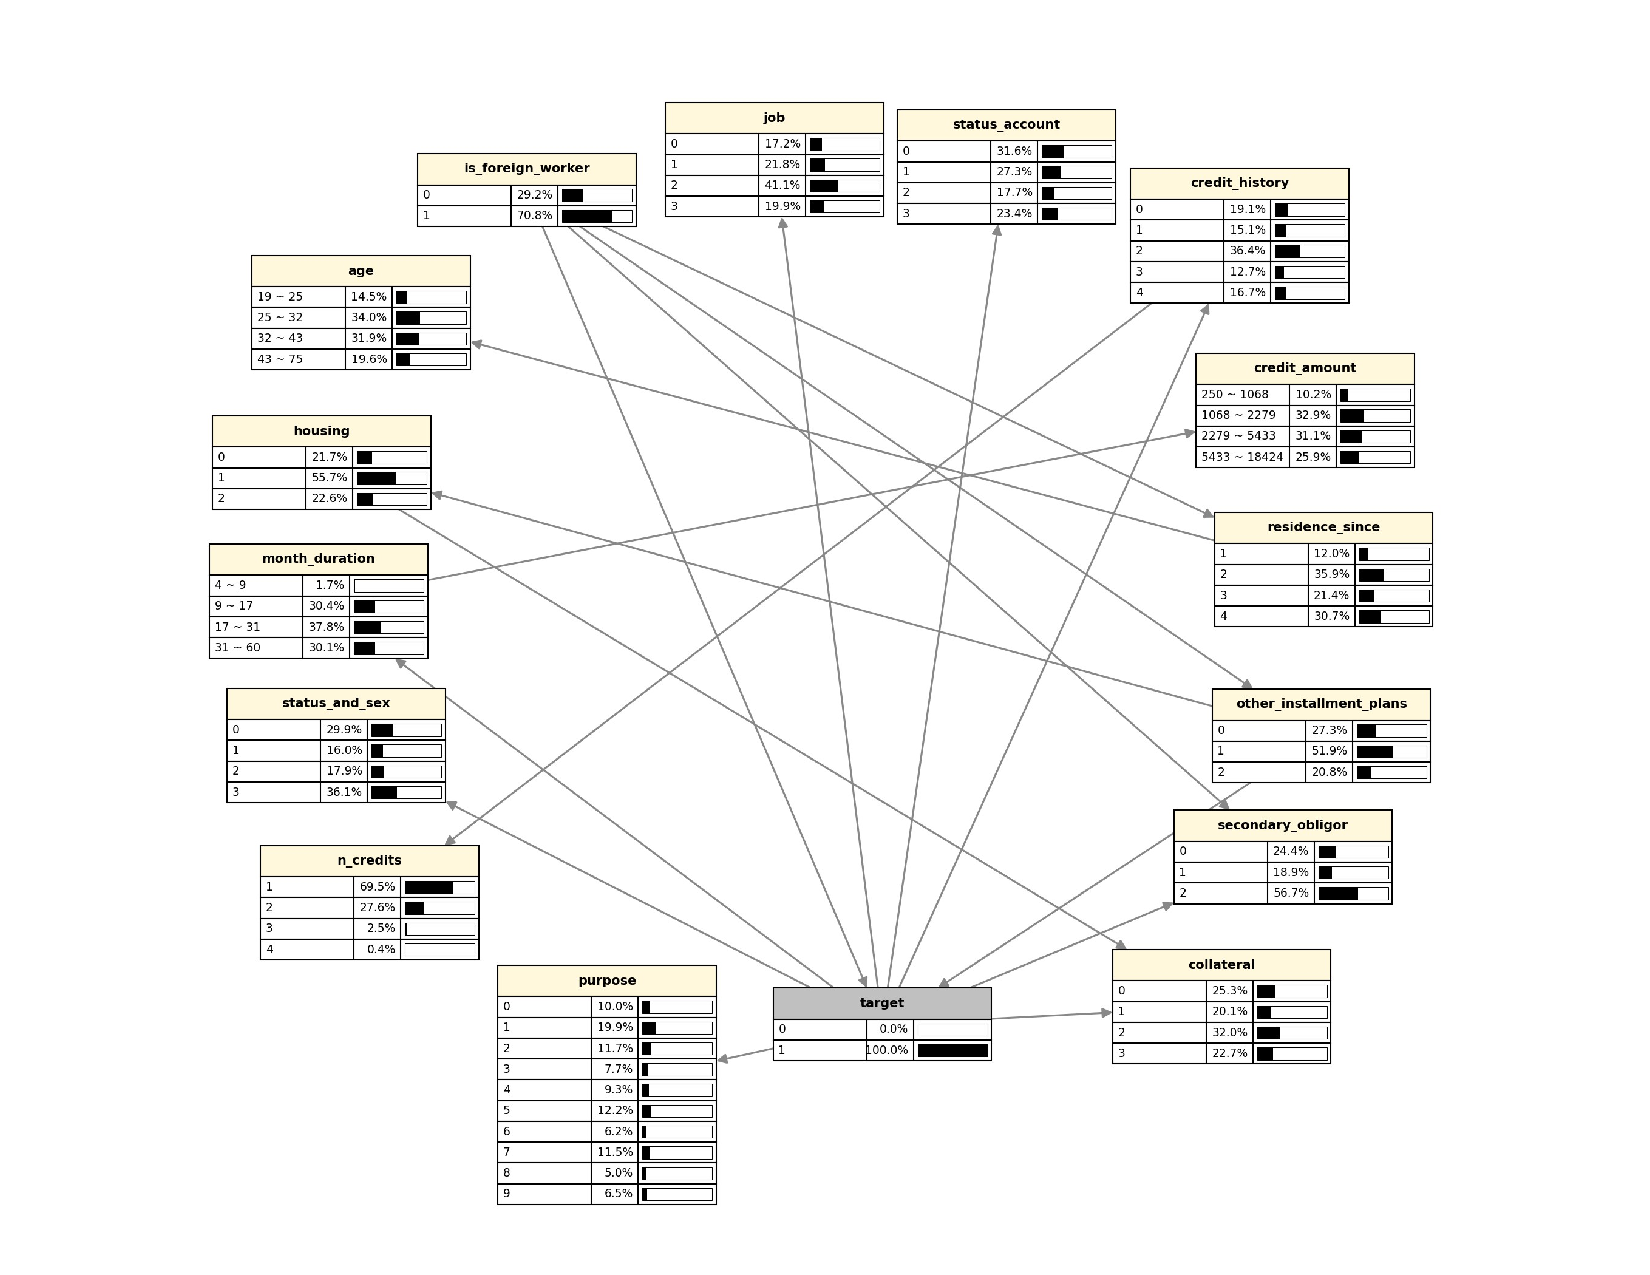
\includegraphics[width=1.2\textwidth,
        height=0.7\textheight,
        trim=3cm 1cm 0cm 1cm,
        clip]{image/backward/ger_back_1.pdf}
        \caption{target = 1}
        \label{fig:ger_back_1}
    \end{subfigure}
    \caption{Suy luận lùi toàn cục theo evidence target --- German Credit (tiếp theo)}
    \label{fig:backward_german}
\end{figure}


Kết quả suy luận lùi toàn cục này nhất quán hoàn toàn với các phát hiện cục bộ đã trình bày ở phần trên, đồng thời cho thấy rõ hơn mức độ lan tỏa của bằng chứng \texttt{target} qua toàn bộ cấu trúc mạng.

Tổng hợp cả ba bộ dữ liệu, suy luận lùi cung cấp một góc nhìn bổ trợ quan trọng so với hai kỹ thuật trước: thay vì trả lời ``một hồ sơ cụ thể có rủi ro bao nhiêu'', nó trả lời ``một nhóm hồ sơ đã biết kết quả thường có đặc điểm gì'', phục vụ trực tiếp cho bài toán truy vết hồ sơ và xây dựng chân dung rủi ro sau khi đã quan sát được kết quả vỡ nợ trên thực tế.


\begin{figure}[p]
    \centering
    \begin{subfigure}[b]{\textwidth}
        \centering
    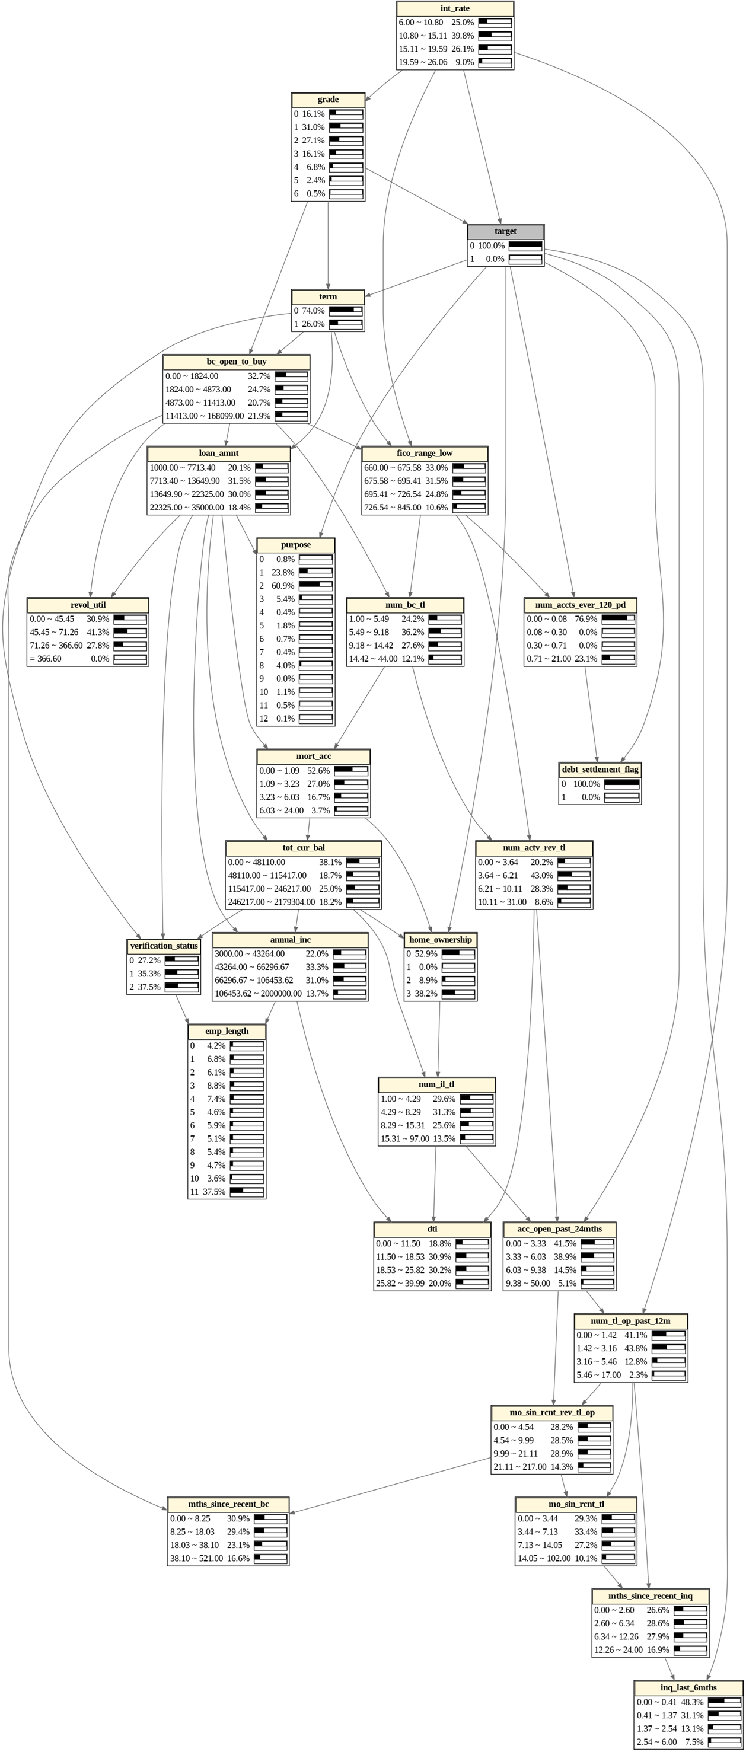
\includegraphics[width=\textwidth,height=\textheight]{image/backward/lend_back_0.pdf}
        \caption{target = 0}
        \label{fig:lend_back_0}
    \end{subfigure}
    \caption{Suy luận lùi toàn cục theo evidence target --- Lending Club}
\end{figure}

\begin{figure}[p]
    \ContinuedFloat
    \centering
    \begin{subfigure}[b]{\textwidth}
        \centering    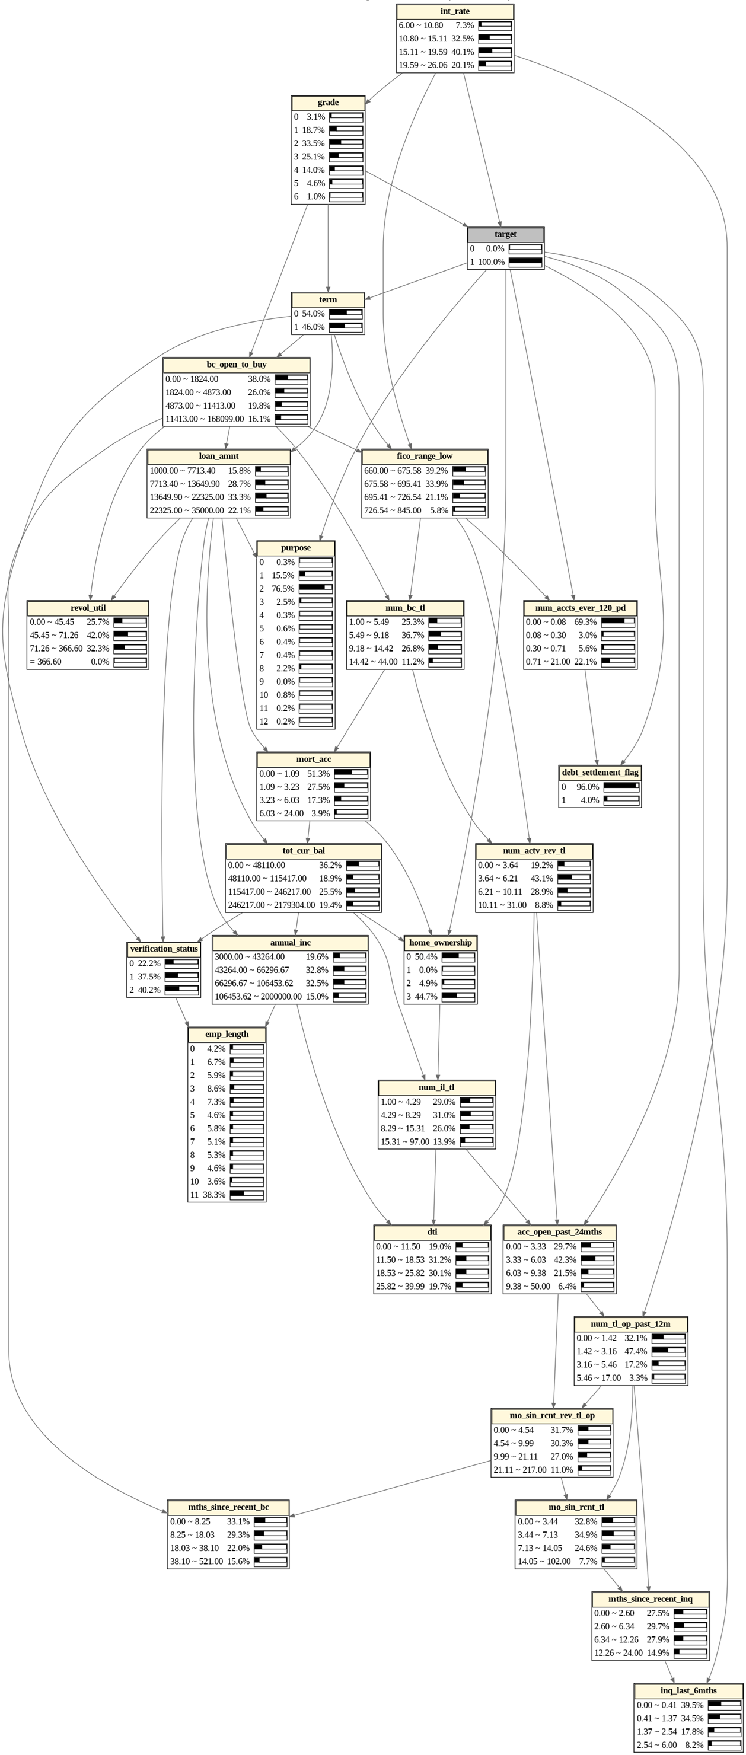
\includegraphics[width=\textwidth,height=\textheight]{image/backward/lend_back_1.pdf}
        \caption{target = 1}
        \label{fig:lend_back_1}
    \end{subfigure}
    \caption{Suy luận lùi toàn cục theo evidence target --- Lending Club (tiếp theo)}
    \label{fig:backward_lendingclub}
\end{figure}

\newpage
\subsubsection{Phân tích kịch bản giả định}
\noindent
Hai cách tiếp cận được triển khai song song để phân tích kịch bản giả định: một cách xét trên hồ sơ cá nhân cụ thể, một cách xét trên cấu trúc con của mạng.

\paragraph{Kịch bản theo hồ sơ cá nhân (Persona-based)}\\

Với mỗi bộ dữ liệu, một vài biến nhân khẩu học không thể can thiệp được cố định làm hồ sơ neo (Australian: \texttt{Age}, \texttt{Citizen}; German: \texttt{age}, \texttt{status\_and\_sex}, \texttt{housing}; Lending Club: \texttt{annual\_inc}, \texttt{fico\_range\_low}, \texttt{mort\_acc}), sau đó lần lượt thay đổi từng biến trong nhóm ba biến nhạy cảm nhất và quan sát $\Delta P(\text{target}=1)$ so với baseline của hồ sơ neo đó.


\begin{figure}[H]
\centering
\begin{subfigure}[b]{\textwidth}
    \centering
    \begin{subfigure}[b]{0.45\textwidth}
        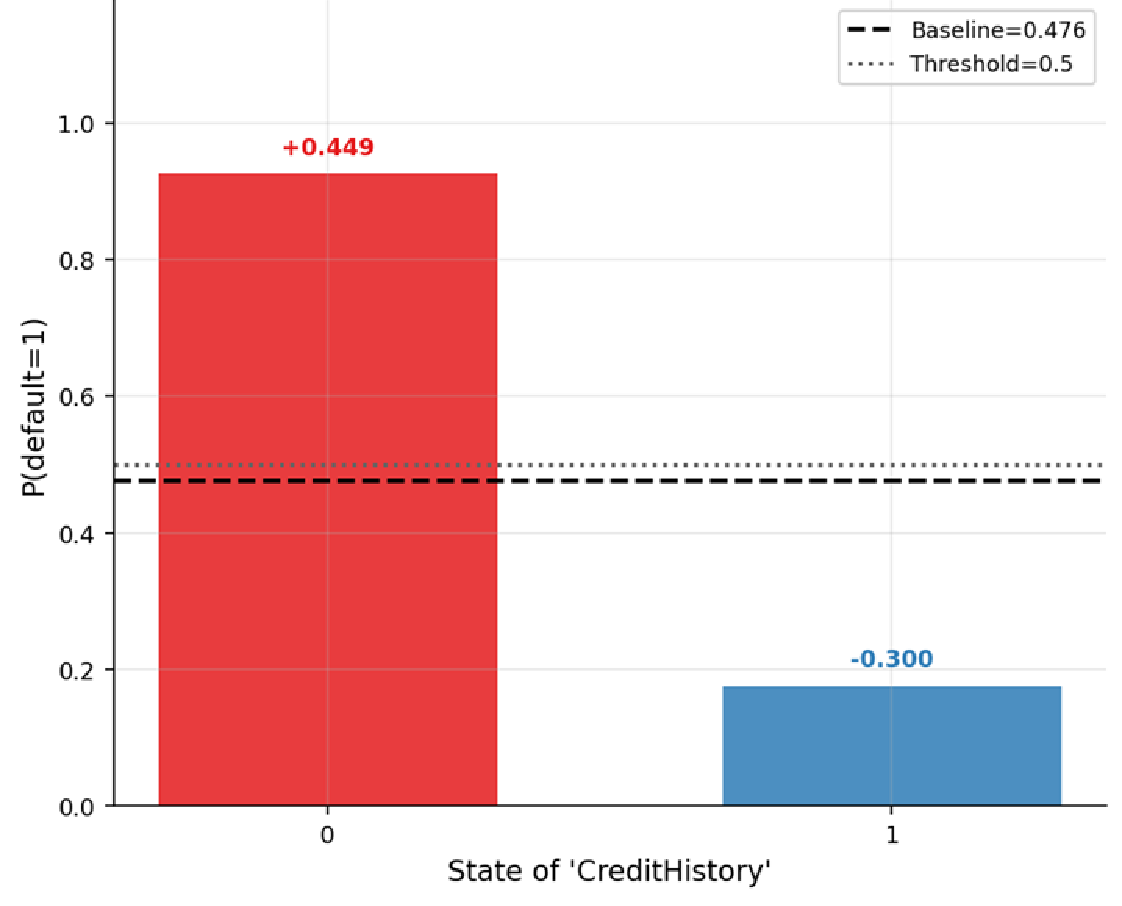
\includegraphics[width=\textwidth]{image/whatif/persona/au_1_crehis.pdf}
    \end{subfigure}
    \hfill
    \begin{subfigure}[b]{0.45\textwidth}
        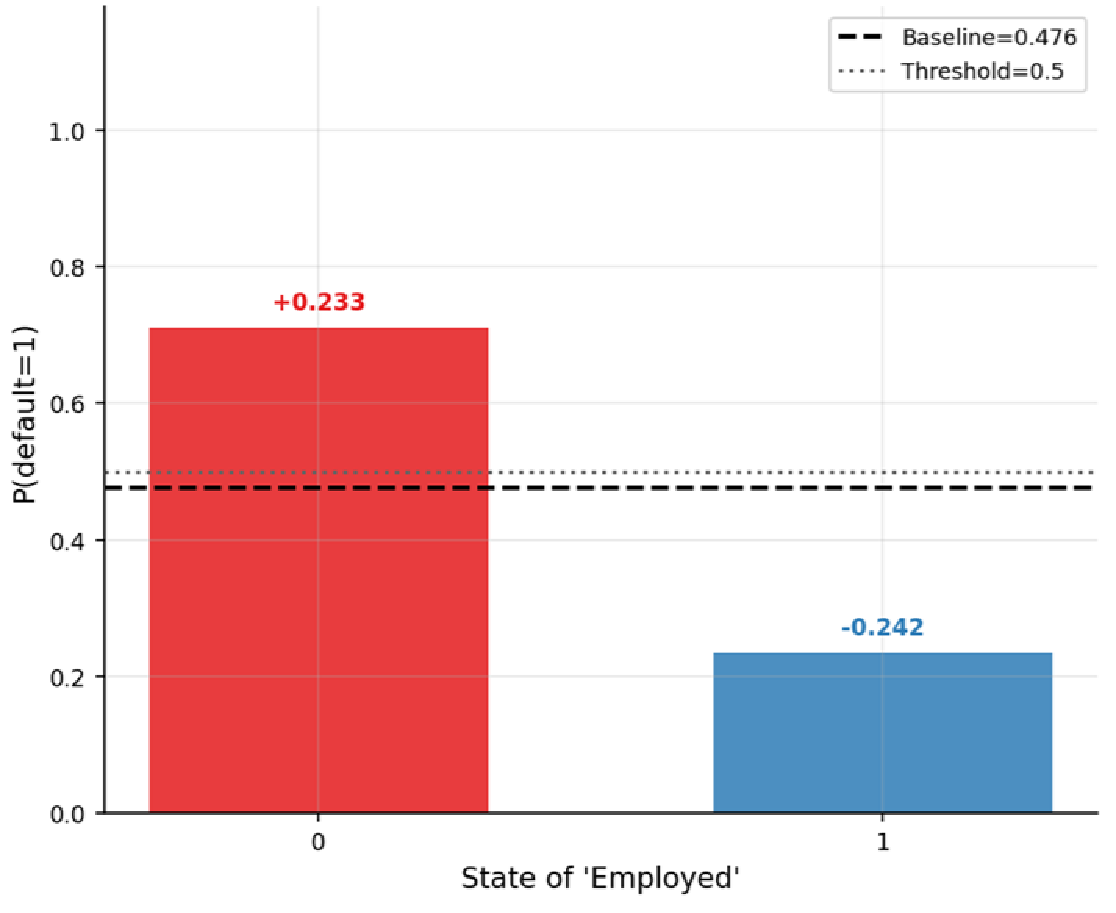
\includegraphics[width=\textwidth]{image/whatif/persona/au_1_employ.pdf}
    \end{subfigure}
    \hfill
    \begin{subfigure}[b]{0.45\textwidth}
        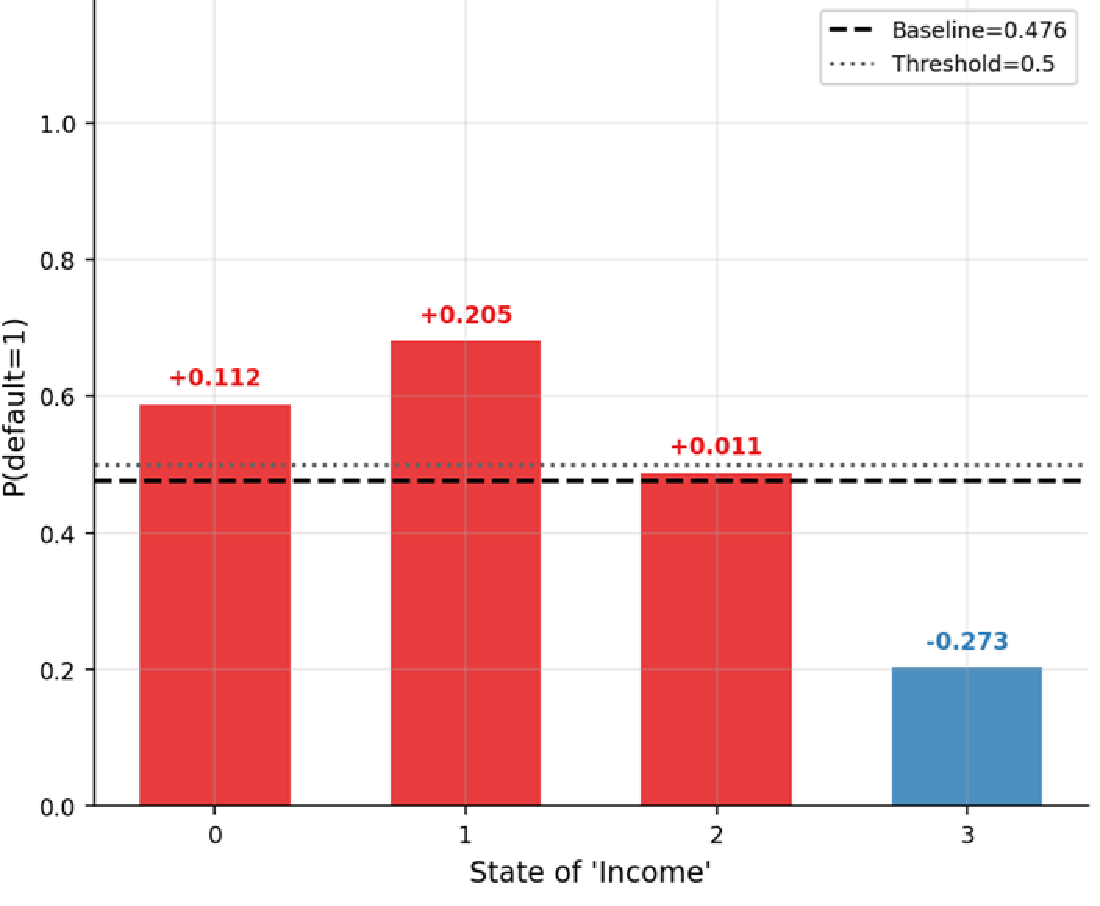
\includegraphics[width=\textwidth]{image/whatif/persona/au_1_inc.pdf}
    \end{subfigure}   
\end{subfigure}

\caption{Phân tích kịch bản giả định theo hồ sơ cá nhân --- Australian Credit {\newline \small (Trong đó, màu xanh: target = 0 và màu đỏ: target = 1})}
\label{fig:whatif_australian}
\end{figure}

Trên Australian Credit, baseline của hồ sơ neo là 47.64\%. Khi \texttt{CreditHistory} chuyển từ "không có" sang "có", xác suất vỡ nợ giảm từ 92.54\% xuống 17.68\% ($\Delta P = -0.300$). \texttt{Employed} cho biên độ nhỏ hơn, giảm từ 70.95\% xuống 23.45\% ($\Delta P = -0.242$) khi chuyển sang có việc làm. \texttt{Income} lại không đơn điệu như đã ghi nhận ở Mục \ref{sec:4.4.1}: xác suất tăng nhẹ từ bin 0 (58.80\%) lên đỉnh ở bin 1 (68.12\%) trước khi giảm dần về bin 3 (20.31\%) (Hình \ref{fig:whatif_australian}).


\begin{figure}[H]
\centering
\begin{subfigure}[b]{\textwidth}
    \centering
    \begin{subfigure}[b]{0.6\textwidth}
        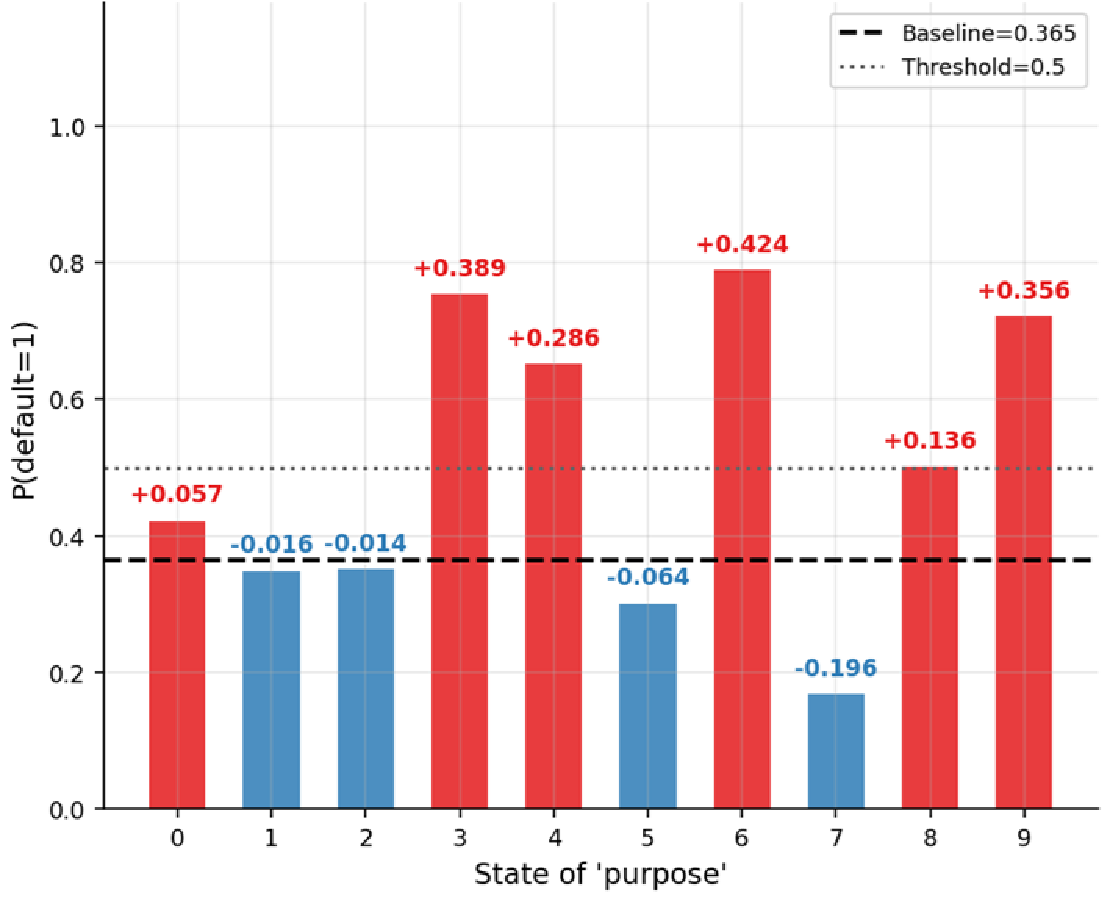
\includegraphics[width=\textwidth]{image/whatif/persona/ger_1_purpose.pdf}
    \end{subfigure}
    \hfill
    \begin{subfigure}[b]{0.6\textwidth}
        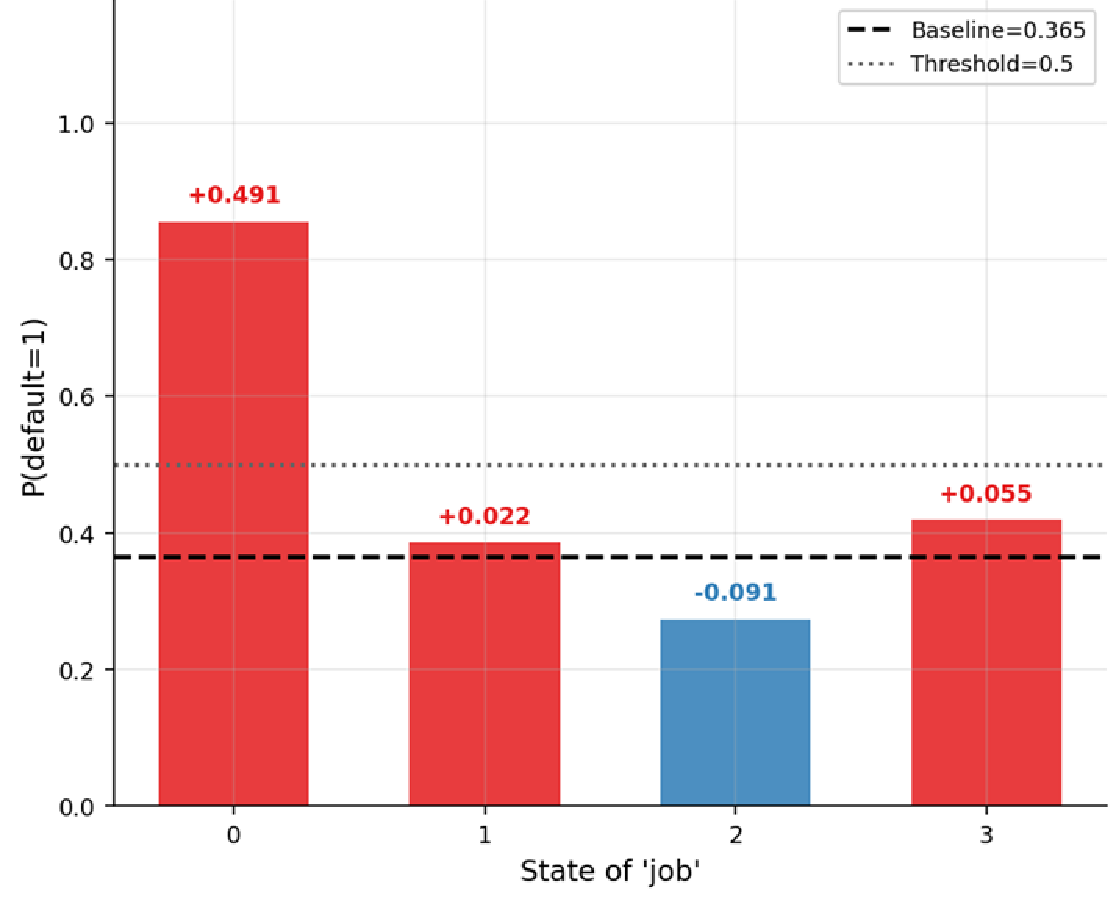
\includegraphics[width=\textwidth]{image/whatif/persona/ger_1_job.pdf}
    \end{subfigure}
    \hfill
    \begin{subfigure}[b]{0.6\textwidth}
        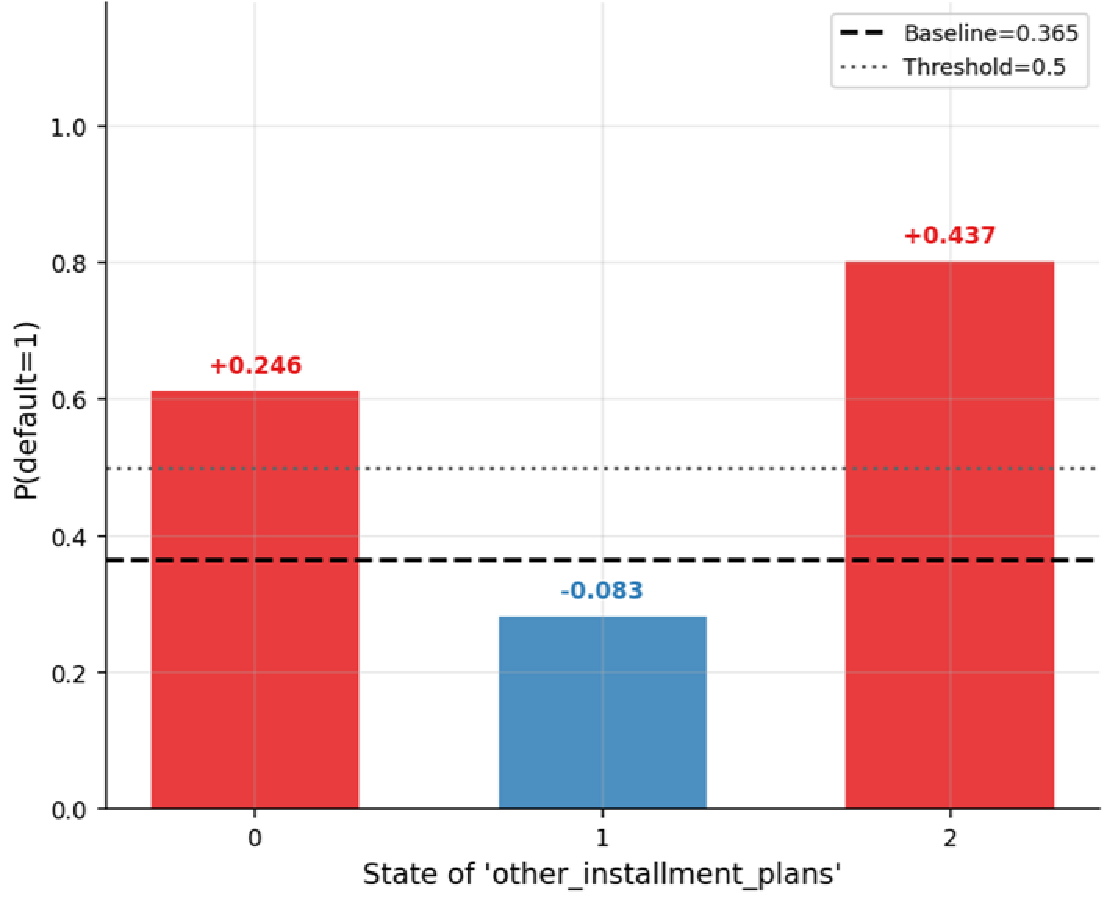
\includegraphics[width=\textwidth]{image/whatif/persona/ger_1_otherins.pdf}
    \end{subfigure}
    \label{fig:whatif_german}
\end{subfigure}

\caption{Phân tích kịch bản giả định theo hồ sơ cá nhân --- German Credit {\newline \small (Trong đó, màu xanh: target = 0 và màu đỏ: target = 1})}
\label{fig:whatif_german}
\end{figure}

\begin{figure}[H]
\centering
\begin{subfigure}[b]{\textwidth}
    \centering
    \begin{subfigure}[b]{0.6\textwidth}
        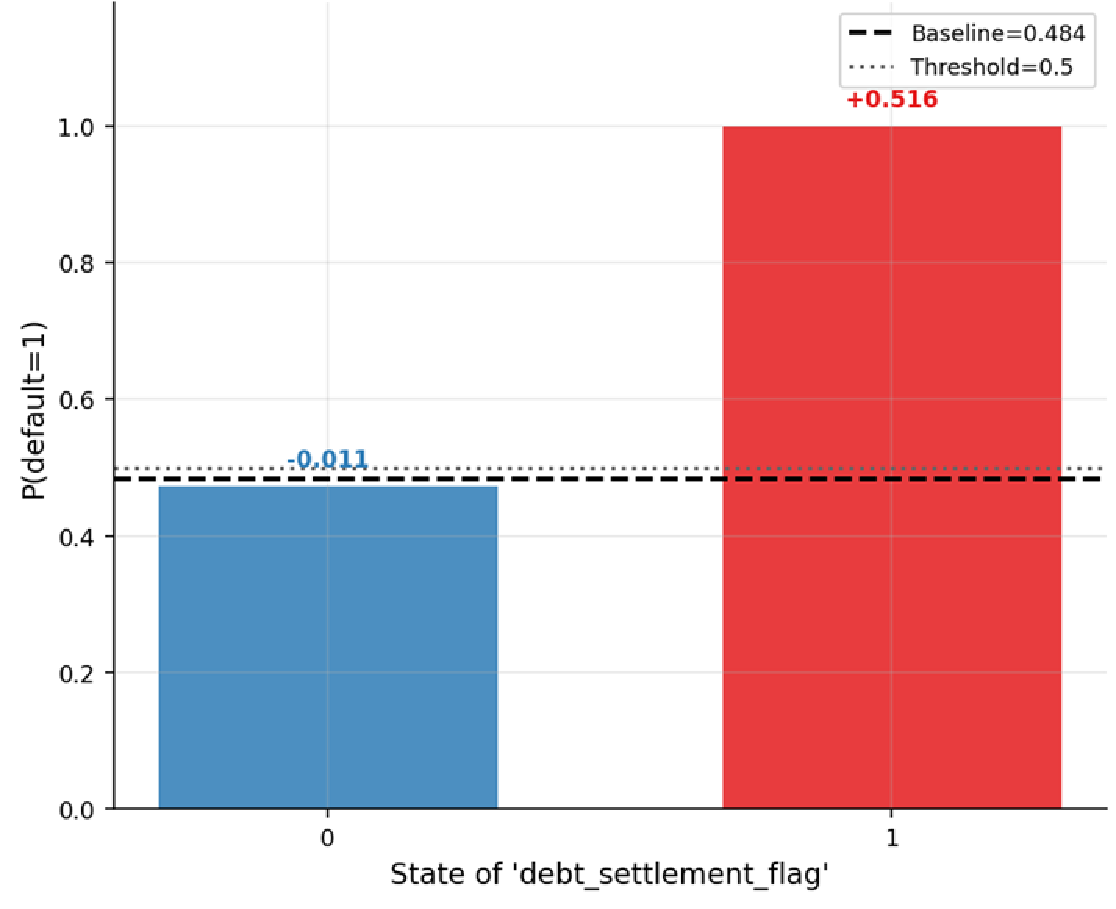
\includegraphics[width=\textwidth]{image/whatif/persona/lend_1_debt.pdf}
    \end{subfigure}
    \hfill
    \begin{subfigure}[b]{0.6\textwidth}
        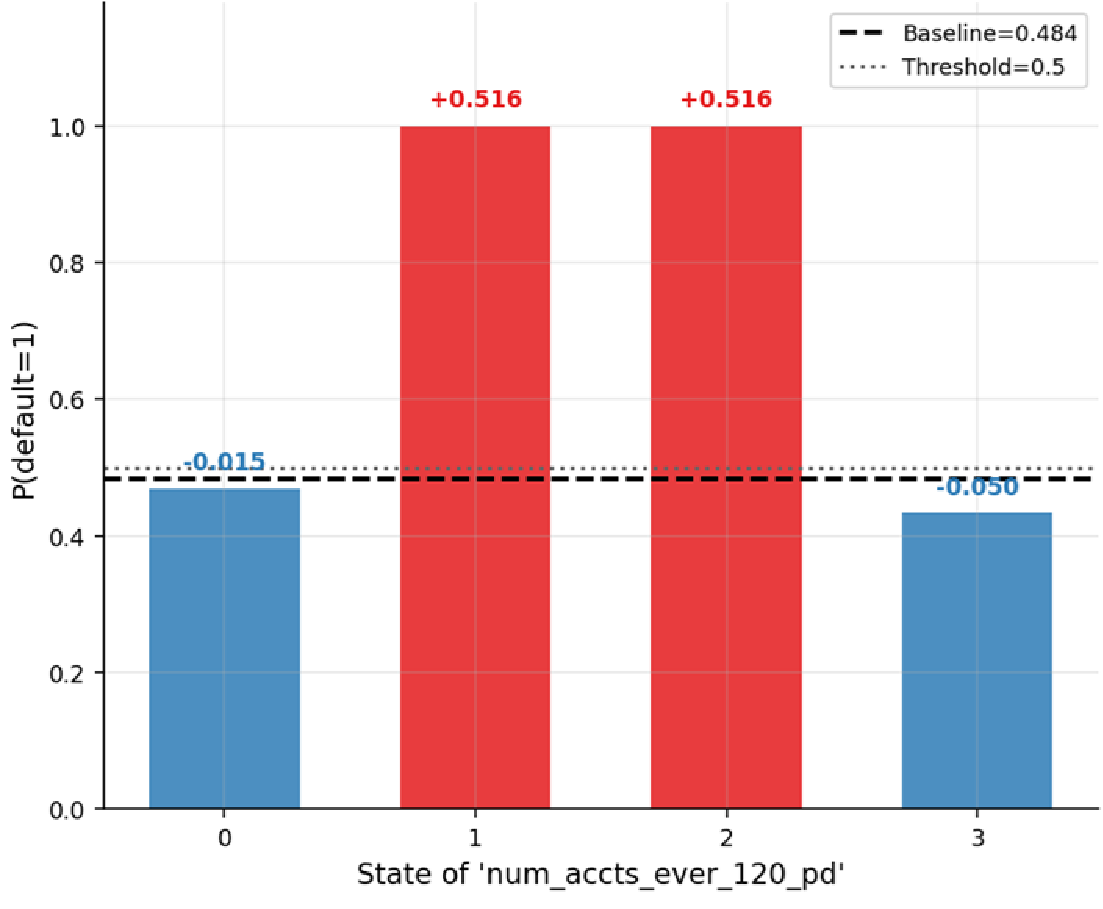
\includegraphics[width=\textwidth]{image/whatif/persona/lend_1_numacc.pdf}
    \end{subfigure}
    \hfill
    \begin{subfigure}[b]{0.6\textwidth}
        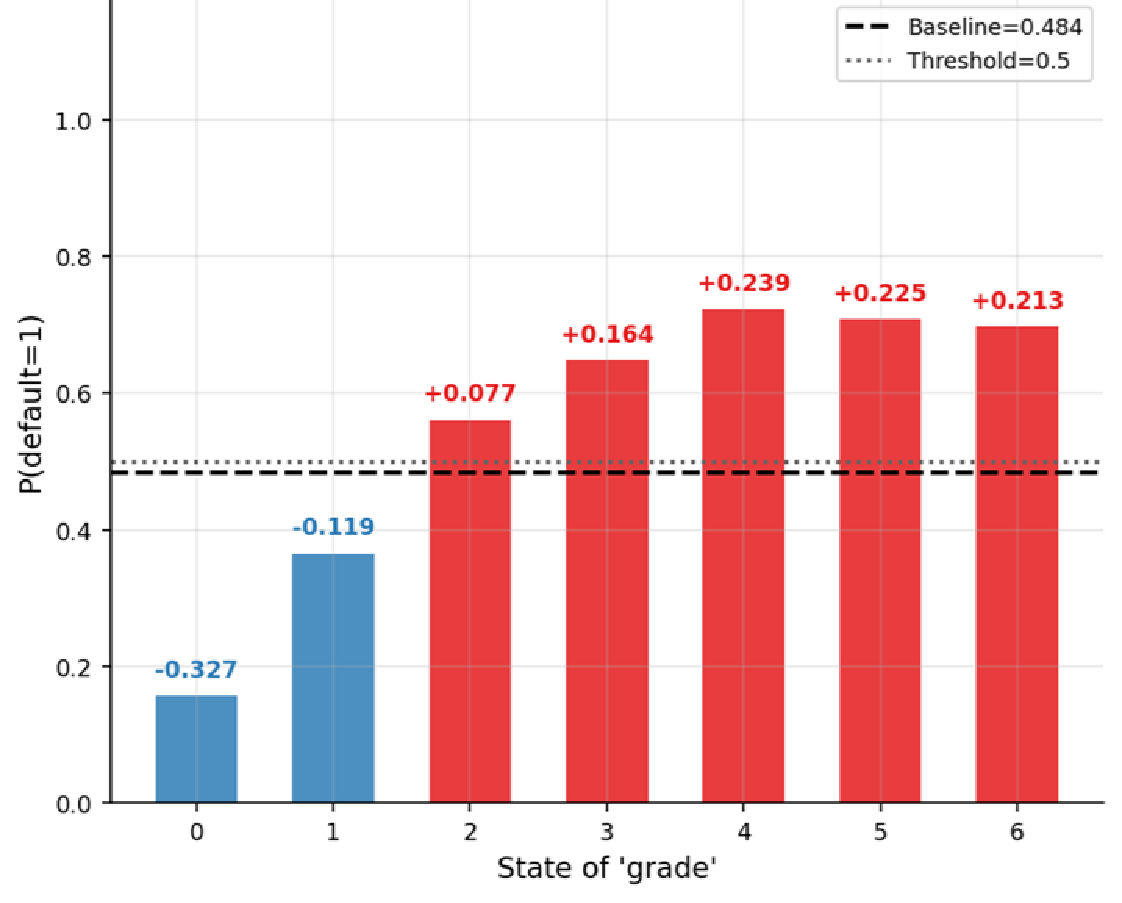
\includegraphics[width=\textwidth]{image/whatif/persona/lend_1_grade.pdf}
    \end{subfigure}
\end{subfigure}

\caption{Phân tích kịch bản giả định theo hồ sơ cá nhân --- Lending Club {\newline \small (Trong đó, màu xanh: target = 0 và màu đỏ: target = 1})}
\label{fig:whatif_lendingclub}
\end{figure}

Trên German Credit, baseline là 36.45\%. \texttt{Purpose} là biến có biên độ lớn nhất trong ba biến được khảo sát, dao động từ 16.84\% (bin 7) đến 78.85\% (bin 6), phản ánh sự phân hóa rủi ro rõ rệt theo từng mục đích vay cụ thể. \texttt{Job} dao động từ 27.35\% đến 85.51\%, trong đó bin 0 (thất nghiệp/không kỹ năng) mang rủi ro cao nhất. \texttt{Other\_installment\_plans} dao động từ 28.13\% (bin "stores") đến 80.10\% (bin "none"), tiếp tục thể hiện hình chữ V phi tuyến đã ghi nhận xuyên suốt các mục trước (Hình \ref{fig:whatif_german}).

Trên Lending Club, baseline là 48.39\%, \varname{num_accts_ever_120_pd} và \varname{Debt_settlement_flag} đều thể hiện biên độ cực đoan giống hệt kết quả $\delta = 0.5$ đã ghi nhận ở Mục \ref{sec:4.4.1}: chuyển sang trạng thái "có" khiến xác suất vỡ nợ nhảy thẳng lên 100\%, một lần nữa xác nhận đây là hệ quả của dữ liệu thưa chứ không phải quan hệ nhân quả ổn định. \texttt{grade} cho biên độ trải rộng và có ý nghĩa diễn giải rõ ràng hơn, giảm xuống thấp nhất 15.73\% ở hạng A và tăng lên cao nhất 72.32\% ở hạng E (Hình \ref{fig:whatif_lendingclub}).

\paragraph{Phân tích cấu trúc con và bảng CPT (Subnetwork)}

Theo cấu trúc DAG đã học được ở Mục \ref{sec: 4.3.1}, với mỗi bộ dữ liệu một cấu trúc con khép kín dạng tam giác quanh target được chọn để dựng bảng CPT đầy đủ.


\begin{figure}[H]
    \centering

     % --- HÀNG 1: Australian Credit ---
    \begin{subfigure}[b]{0.4\textwidth} % Giảm nhẹ xuống 0.8 để 2 hình chắc chắn vừa 1 trang
        \centering
        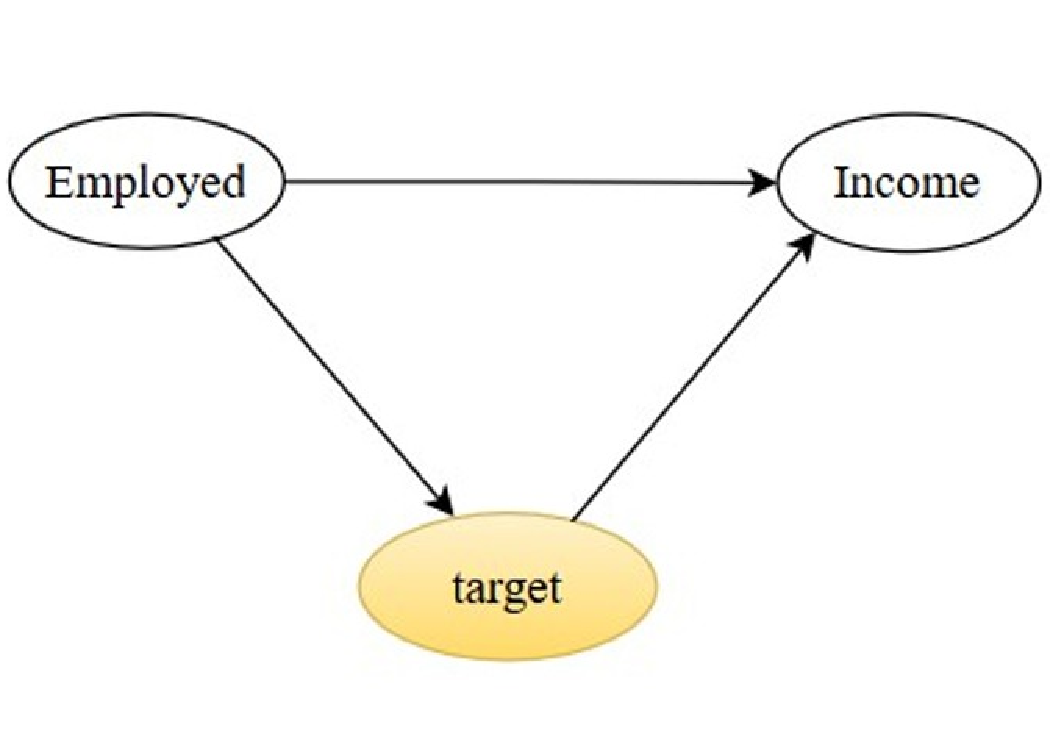
\includegraphics[width=\textwidth]{image/whatif/subnetwork/sub_au.pdf}
        \caption{Đồ thị con của Australian Credit}
        \label{fig:subnet_australian}
    \end{subfigure}
    \hfill
    % --- HÀNG 1: German Credit ---
    \begin{subfigure}[b]{0.45\textwidth}
        \centering
        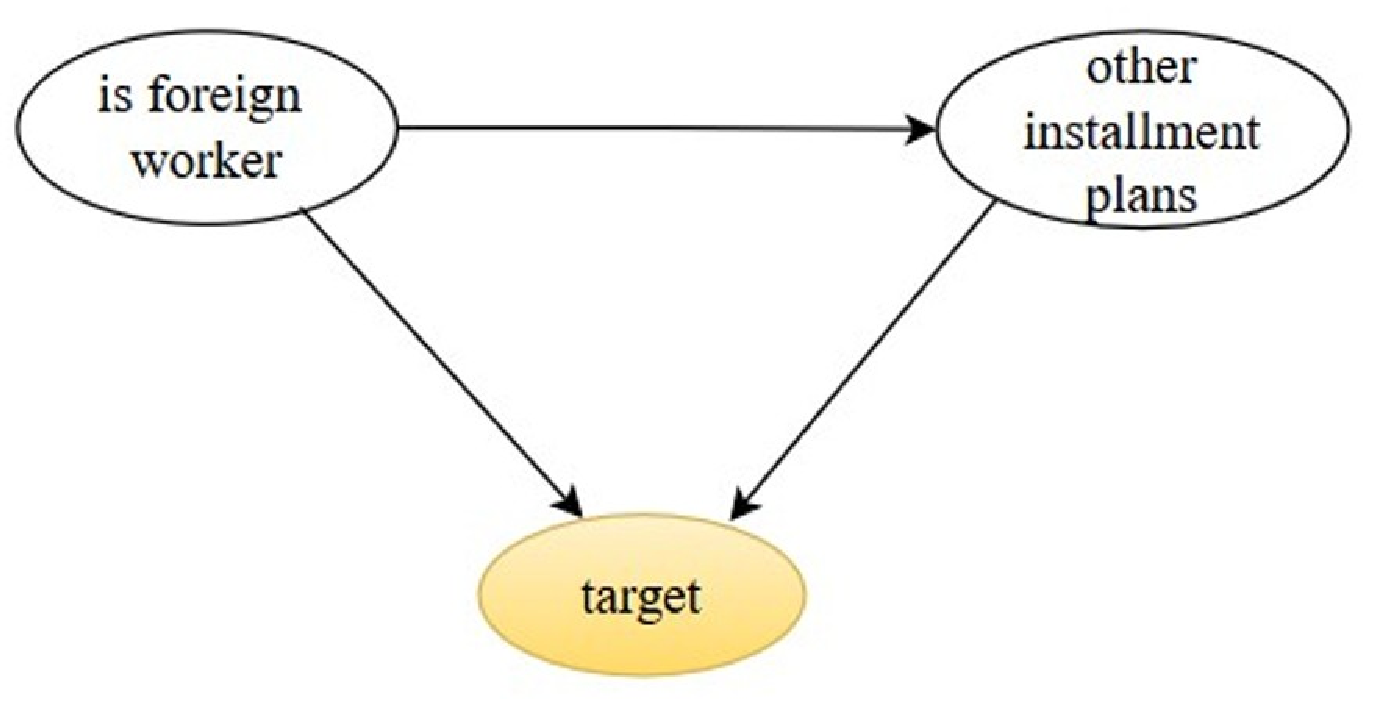
\includegraphics[width=\textwidth,
        height=0.14\textheight,
        trim=0cm 0cm 0cm 2cm,]{image/whatif/subnetwork/sub_ger.pdf}
        \caption{Đồ thị con của German Credit}
        \label{fig:subnet_german}
    \end{subfigure}
    \hfill
    \begin{subfigure}[b]{0.5\textwidth}
         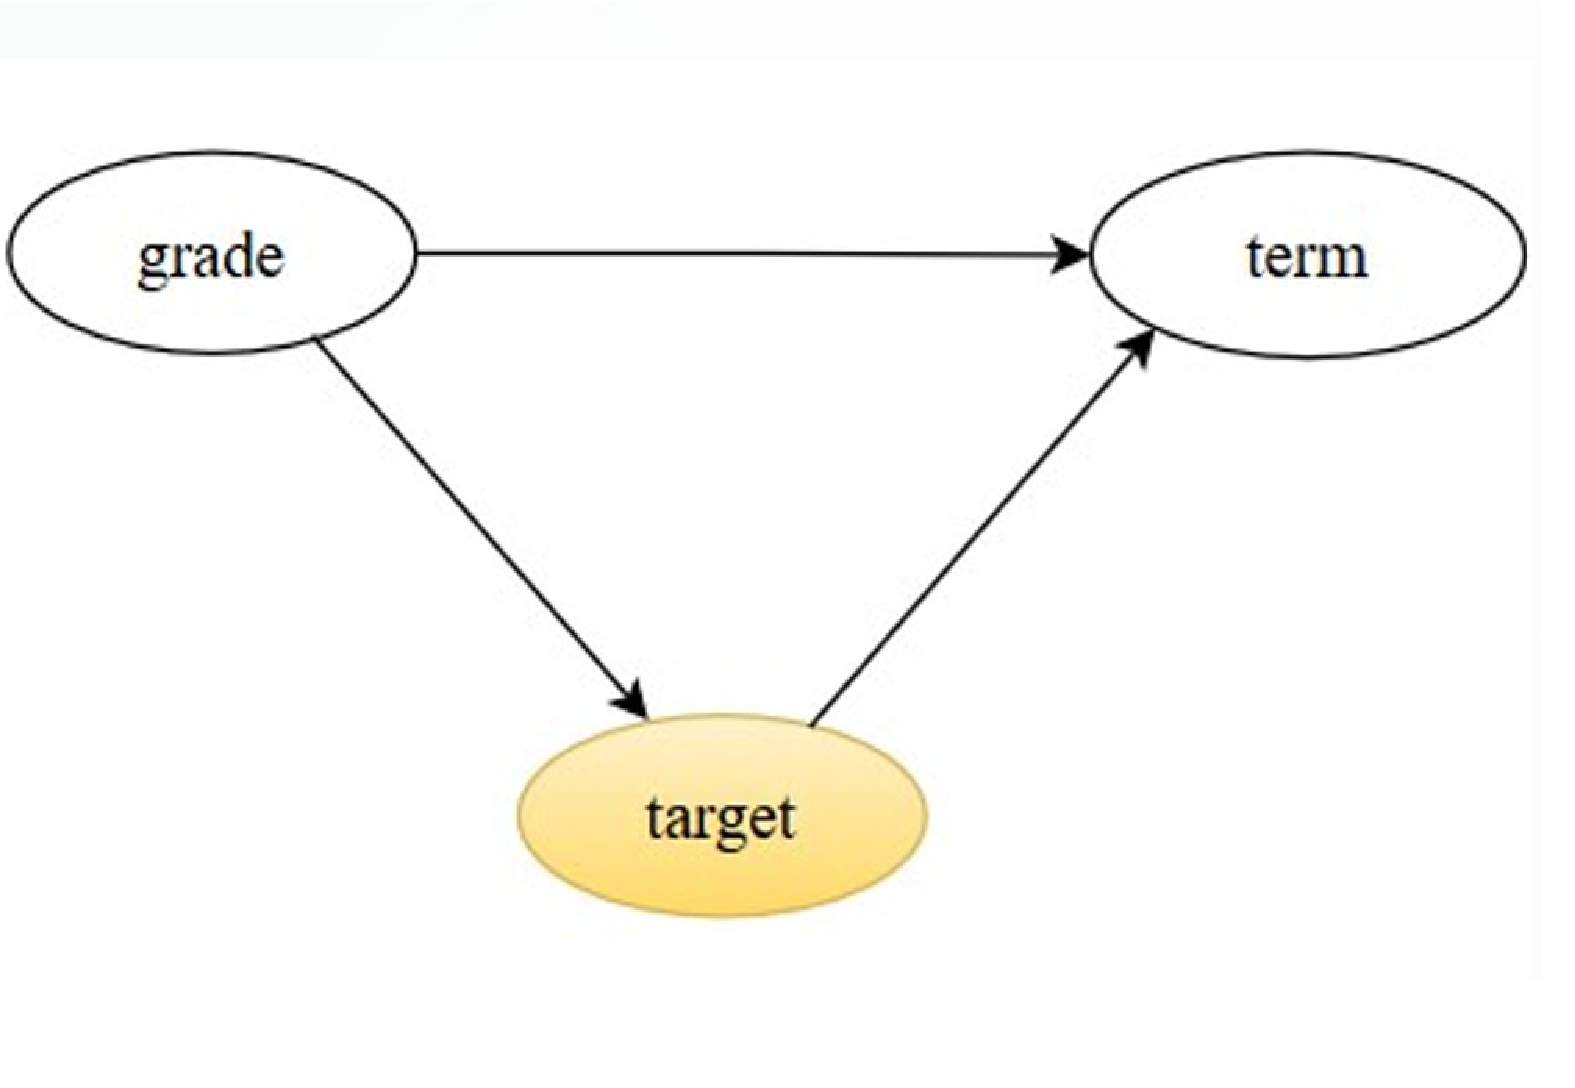
\includegraphics[width=\textwidth,
         height=0.25\textheight]{image/whatif/subnetwork/sub_lend.pdf}
        \caption{Đồ thị con của Lending Club}
        \label{fig:subnet_lendingclub}
    \end{subfigure}

    \caption{Đồ thị con của ba mạng Bayes}
    \label{fig:subnet_structures}

\end{figure}


\FloatBarrier
%%%%%%%%%%%%%%%%%%%%%%%%%%%%%%%
\begin{table}[htbp]
\centering
\caption{CPT của target theo Employed × Income --- Australian Credit}
\label{tab:cpt_australian}
\begin{tabular}{lcccccccc}
\toprule
Employed & 0 & 0 & 0 & 0 & 1 & 1 & 1 & 1 \\
Income   & 0 & 1 & 2 & 3 & 0 & 1 & 2 & 3 \\
\midrule
$P(\text{target}=1)$ & 0.7190 & 0.7474 & 0.7871 & 0.6174 & 0.2455 & 0.6606 & 0.3026 & 0.0441 \\
$P(\text{target}=0)$ & 0.2810 & 0.2526 & 0.2129 & 0.3826 & 0.7545 & 0.3394 & 0.6974 & 0.9559 \\
\bottomrule
\end{tabular}
\end{table}
\FloatBarrier

Trên Australian Credit, cấu trúc con được chọn là \texttt{Employed} (cha) - target - \texttt{Income} (con), khép vòng qua cạnh trực tiếp \texttt{Employed} $\rightarrow$ \texttt{Income} (Hình \ref{fig:subnet_australian}, Bảng \ref{tab:cpt_australian}). Quy tắc rủi ro cao nhất: chưa có việc làm và \texttt{Income} ở bin 2 cho xác suất vỡ nợ cao nhất (78.71\%). Quy tắc rủi ro thấp nhất: đang có việc làm và \texttt{Income} ở bin 3 cho xác suất thấp nhất (4.41\%) chênh lệch hơn 74 điểm phần trăm giữa hai thái cực.

\vspace{1em}
\begin{table}[htbp]
\centering
\caption{CPT của target theo is\_foreign\_worker × other\_installment\_plans --- German Credit}
\label{tab:cpt_german}
\begin{tabular}{lcccccc}
\toprule
is\_foreign\_worker & 0 & 0 & 0 & 1 & 1 & 1 \\
other\_installment\_plans & 0 & 1 & 2 & 0 & 1 & 2 \\
\midrule
$P(\text{target}=1)$ & 1.0000 & 0.6491 & 1.0000 & 0.5948 & 0.3482 & 0.7705 \\
$P(\text{target}=0)$ & 0.0000 & 0.3509 & 0.0000 & 0.4052 & 0.6518 & 0.2295 \\
\bottomrule
\end{tabular}
\end{table}


\vspace{1em}
\begin{table}[htbp]
\centering
\caption{CPT của target theo grade × term --- Lending Club}
\label{tab:cpt_lendingclub}
\begin{tabular}{lcccccccc}
\toprule
grade & 0 & 0 & 1 & 1 & 2 & 2 & 3 & 3 \\
term  & 0 & 1 & 0 & 1 & 0 & 1 & 0 & 1 \\
\midrule
$P(\text{target}=1)$ & 0.1515 & 0.3977 & 0.3528 & 0.5214 & 0.5109 & 0.6186 & 0.5645 & 0.6579 \\
$P(\text{target}=0)$ & 0.8485 & 0.6023 & 0.6472 & 0.4786 & 0.4891 & 0.3814 & 0.4355 & 0.3421 \\
\midrule
grade & 4 & 4 & 5 & 5 & 6 & 6 & & \\
term  & 0 & 1 & 0 & 1 & 0 & 1 & & \\
\midrule
$P(\text{target}=1)$ & 0.6255 & 0.6961 & 0.5829 & 0.6802 & 0.6111 & 0.6723 & & \\
$P(\text{target}=0)$ & 0.3745 & 0.3039 & 0.4171 & 0.3198 & 0.3889 & 0.3277 & & \\
\bottomrule
\end{tabular}
\end{table}


\vspace{1em}
Trên German Credit, cấu trúc con được chọn là \texttt{is\_foreign\_worker} và \texttt{other\_installment\_plans}, hai biến cha có liên kết trực tiếp với nhau, cùng khép vòng qua target (Hình \ref{fig:subnet_german}, Bảng \ref{tab:cpt_german}). Hai tổ hợp đạt xác suất vỡ nợ tuyệt đối 100\% đều rơi vào nhóm lao động nước ngoài (\texttt{is\_foreign\_worker}=0, quy ước "Yes"), dù ở hai trạng thái trái ngược của \texttt{other\_installment\_plans} ("Bank" và "none"). Quy tắc rủi ro thấp nhất là không phải lao động nước ngoài kết hợp "stores" (34.82\%).

Trên Lending Club, cấu trúc con được chọn là \texttt{grade} (cha) - target - \texttt{term} (con), khép vòng qua cạnh trực tiếp \texttt{grade} $\rightarrow$ \texttt{term} (Hình \ref{fig:subnet_lendingclub}, Bảng \ref{tab:cpt_lendingclub}). Ở mọi hạng tín dụng, kỳ hạn vay 60 tháng luôn mang xác suất vỡ nợ cao hơn kỳ hạn 36 tháng, và mức chênh lệch này khá ổn định qua các hạng (dao động 6--25 điểm phần trăm), cho thấy \texttt{term} tác động cộng dồn tương đối đều đặn lên \texttt{grade} thay vì tạo ra tương tác khuếch đại như cặp biến ở German Credit.

Tổng hợp cả hai cách tiếp cận, phương pháp persona-based phù hợp khi mục tiêu là tư vấn can thiệp cho một hồ sơ cụ thể, kết quả trực quan và dễ diễn giải bằng $\Delta P$ so với một baseline cố định, nhưng chỉ phản ánh đúng cho đúng hồ sơ neo đã chọn. Ngược lại, phương pháp subnetwork/CPT cho một bức tranh toàn cục về mọi tổ hợp trạng thái có thể xảy ra giữa hai biến có quan hệ cấu trúc trực tiếp, phù hợp để rút ra quy tắc quản trị rủi ro ở cấp độ chính sách thay vì cho một cá nhân cụ thể. Việc kết hợp cả hai cách tiếp cận, như đã thực hiện trong khóa luận, cho phép vừa phục vụ nhu cầu tư vấn cá nhân hóa vừa cung cấp cơ sở hoạch định chính sách tín dụng ở quy mô tổng thể.


\subsubsection{So sánh với LIME/SHAP}
\noindent
Với mỗi bộ dữ liệu, một khách hàng được chọn ngẫu nhiên và giải thích đồng thời bằng ba cách: LIME, SHAP, và biểu đồ diễn giải của Mạng Bayes, gán từng biến làm evidence theo đúng thứ tự các nút trong đồ thị và ghi nhận mức thay đổi xác suất hậu nghiệm sau mỗi bước.

Trên Australian Credit, khách hàng được chọn có xác suất vỡ nợ $87,6\%$, chưa có lịch sử tín dụng, chưa có việc làm, và biến \textit{Income} nằm ở bin cao nhất. Cả ba phương pháp diễn giải đều thống nhất \textit{CreditHistory} là yếu tố chi phối chính làm tăng rủi ro vỡ nợ: LIME gán $+65,4\%$, Mạng Bayes gán $+42,4\%$. Với SHAP, $\textit{CreditHistory} = 0.0$ và $\textit{Income} = 3.0$ là hai biến nằm về phía đẩy dự đoán lên cao, trong đó \textit{CreditHistory} nằm sát ranh giới quyết định $f(x) = 0.88$ — vị trí phản ánh vai trò chi phối của biến này đối với kết quả dự đoán cuối cùng. Sự đồng thuận của cả ba phương pháp về biến chi phối, dù mỗi phương pháp dựa trên cơ chế toán học khác nhau, củng cố độ tin cậy của kết luận rằng tình trạng thiếu lịch sử tín dụng là nguyên nhân chính dẫn đến đánh giá rủi ro cao đối với hồ sơ này.

Trên German Credit, khách hàng được chọn có xác suất vỡ nợ 5.3\% (Hình \ref{fig:explain_german}). Cả ba phương pháp đều thống nhất chiều tác động chung ở \texttt{other\_installment\_plans}, \texttt{secondary\_obligor}, \texttt{job} và \texttt{status\_and\_sex} (đều làm giảm rủi ro). Tuy nhiên có hai điểm bất đồng đáng chú ý. Thứ nhất, \texttt{credit\_history}: LIME không đưa biến này vào top 7 quan trọng nhất, trong khi Mạng Bayes gán $+10.6\%$ (mức tăng rủi ro lớn nhất hồ sơ) và SHAP cũng xác nhận \texttt{credit\_history} = 1.0 là đoạn hồng. Thứ hai, \texttt{housing}: LIME ($+8.0\%$) và SHAP (đoạn hồng rõ rệt cho \texttt{housing} = 0.0) đều xem đây là yếu tố làm tăng rủi ro, nhưng biến này lại hoàn toàn biến mất khỏi biểu đồ diễn giải của Mạng Bayes, tức đóng góp của nó dưới ngưỡng ghi nhận tại đúng thời điểm được thêm vào chuỗi bằng chứng tuần tự.

Trên Lending Club, khách hàng được chọn có xác suất vỡ nợ rất thấp, chỉ 3.4\%, với \texttt{debt\_settlement\_flag} ở trạng thái "không" (0), trái ngược với hồ sơ rủi ro cực trị đã phân tích trước đó. LIME vẫn xếp \texttt{debt\_settlement\_flag} $\leq$ 0.00 là yếu tố làm giảm rủi ro mạnh nhất ($-21.4\%$), trong khi Mạng Bayes lại cho thấy vai trò của biến này gần như không đáng kể ($-0.4\%$) và thay vào đó xác định \texttt{int\_rate} = 0 mới là yếu tố chi phối chính ($-28.1\%$), theo sau là \texttt{grade} = 0 ($-11.1\%$); SHAP cũng đồng thuận với Mạng Bayes khi \texttt{int\_rate} = 0.0 chiếm phần lớn đoạn màu xanh (giảm rủi ro), còn \texttt{debt\_settlement\_flag} không đủ ngưỡng để xuất hiện trong biểu đồ. Sự bất đối xứng này giữa hai trạng thái của \texttt{debt\_settlement\_flag} rất đáng chú ý: khi ở trạng thái hiếm gặp (= 1, đang trong chương trình tái cơ cấu nợ), biến này gần như quyết định tuyệt đối kết quả như đã ghi nhận ở hồ sơ trước (Mạng Bayes $+54.6\%$); nhưng khi ở trạng thái phổ biến (= 0, không tái cơ cấu), nó chỉ mang rất ít thông tin bổ sung so với những gì \texttt{int\_rate} và \texttt{grade} đã thể hiện, vì phần lớn khách hàng vốn dĩ đã ở trạng thái này. LIME dường như không phân biệt được sự bất đối xứng này vì phương pháp xấp xỉ tuyến tính cục bộ gán trọng số dựa trên mức độ nhiễu loạn xung quanh điểm dữ liệu chứ không phản ánh đúng phân phối thực của biến trong toàn bộ tập dữ liệu.

Tổng hợp cả ba bộ dữ liệu, cả ba phương pháp nhìn chung thống nhất về chiều tác động và biến chi phối chính của từng hồ sơ, cho thấy cấu trúc nhân quả mà mạng Bayes học được không mâu thuẫn với các phép xấp xỉ hậu kiểm phổ biến. Tuy nhiên, độ lớn đóng góp cụ thể (trong trường hợp German Credit là cả chiều tác động của một vài biến) không đồng nhất giữa ba phương pháp, đặc biệt khi bảng CPT liên quan đến dữ liệu thưa hoặc khi ảnh hưởng của một biến phụ thuộc mạnh vào các biến khác đã được cố định trước đó trong chuỗi lan truyền bằng chứng. Ngoài ra, thứ tự trình bày các biến trong Mạng Bayes phụ thuộc vào thứ tự các nút trong đồ thị chứ không tự động sắp xếp theo độ lớn đóng góp như LIME hay SHAP, nên một số biến quan trọng có thể xuất hiện ở vị trí giữa biểu đồ thay vì đầu bảng. Đây là một khác biệt về cách trình bày cần lưu ý khi so sánh trực tiếp ba phương pháp, hơn là một khác biệt về bản chất suy luận.

\begin{figure}[H]
\centering
{\small \textbf{Xác suất dự đoán}: Is default ~=~0.8762, No default~=~0.1238}\\[0.3em]
\vspace{0.8em}
\begin{subfigure}[b]{0.9\textwidth}
    \centering
    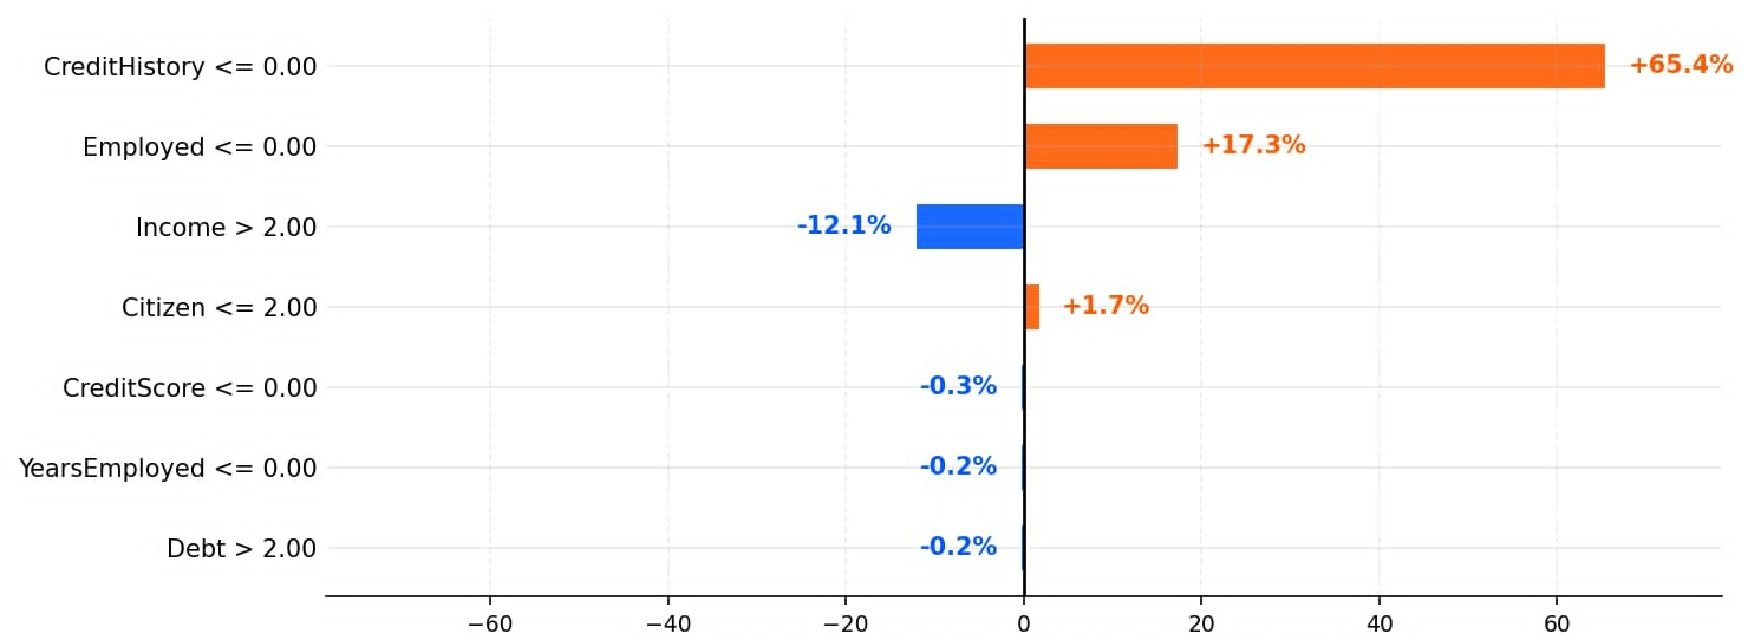
\includegraphics[width=\textwidth]{image/limeshap/au_lime_1.pdf}
    \caption{LIME}
    \label{fig:au_lime}
\end{subfigure}
\vspace{0.8em}
\begin{subfigure}[b]{0.7\textwidth}
    \centering
    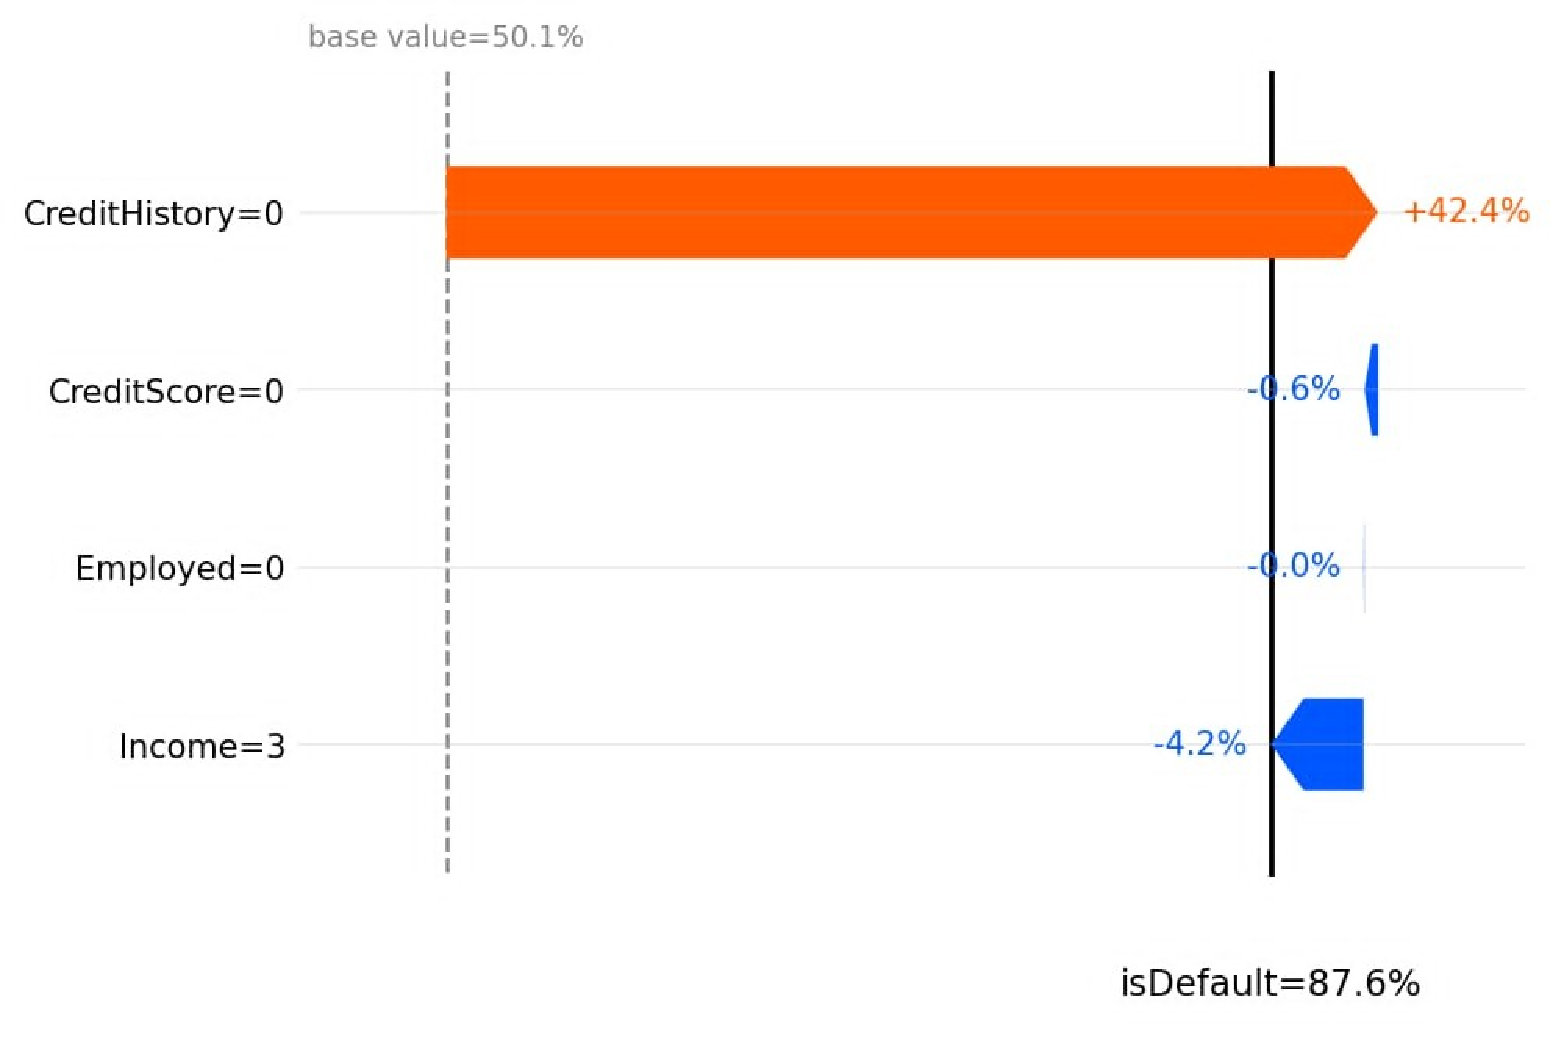
\includegraphics[width=\textwidth]{image/limeshap/au_lime_2.pdf}
    \caption{Mạng Bayes}
    \label{fig:au_waterfall}
\end{subfigure}
\vspace{0.8em}
\begin{subfigure}[b]{1.1\textwidth}
    \centering
    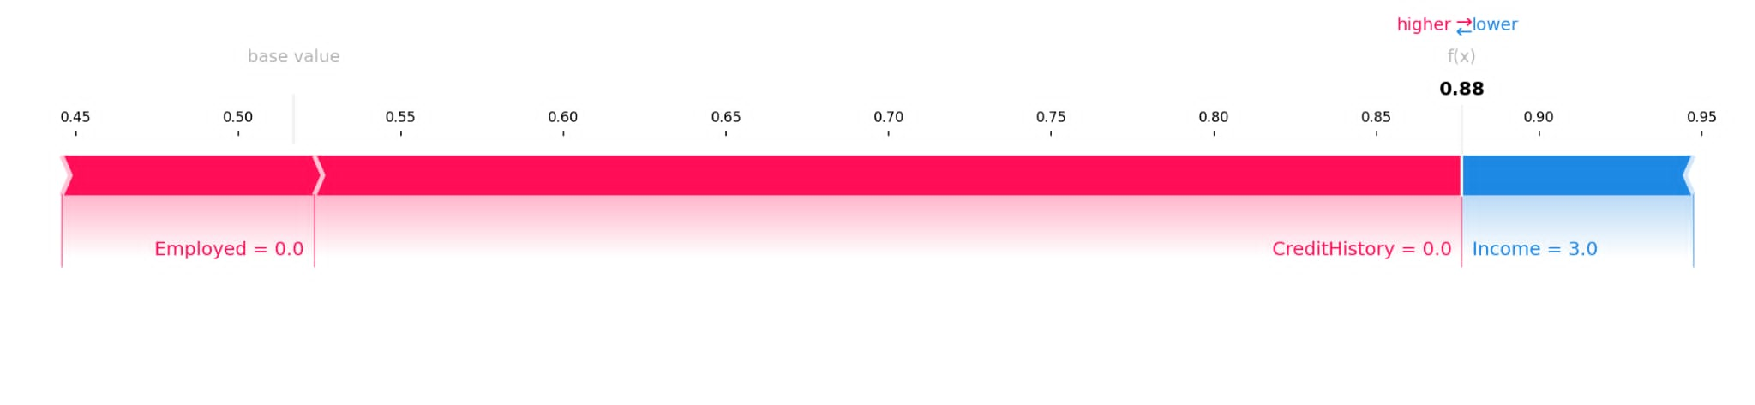
\includegraphics[width=\textwidth,
        height=0.18\textheight,
        trim=1cm 2cm 0cm 0cm,
        clip]{image/limeshap/au_shap.pdf}
    \caption{SHAP}
    \label{fig:au_shap}
\end{subfigure}
\caption{So sánh ba phương pháp giải thích cục bộ cho một hồ sơ khách hàng ngẫu nhiên --- Australian Credit}
\label{fig:explain_australian}
\end{figure}

\begin{figure}[htbp]
\centering
{\small \textbf{Xác suất dự đoán}: Is default ~=~0.0526, No default~=~0.9474}\\[0.3em]

\vspace{0.8em}
\begin{subfigure}[b]{1\textwidth}
    \centering
    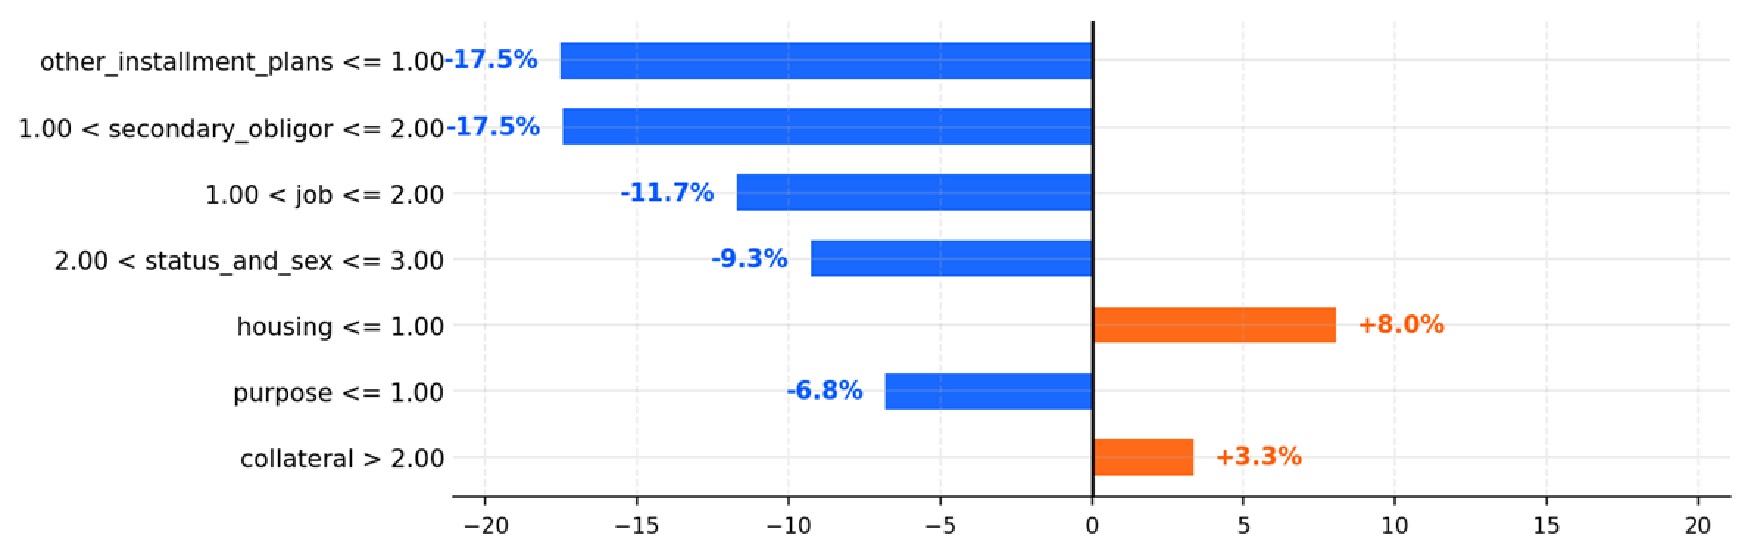
\includegraphics[width=\textwidth]{image/limeshap/ger_lime_1.pdf}
    \caption{LIME}
    \label{fig:ger_lime}
\end{subfigure}
\vspace{0.8em}
\begin{subfigure}[b]{0.8\textwidth}
    \centering
    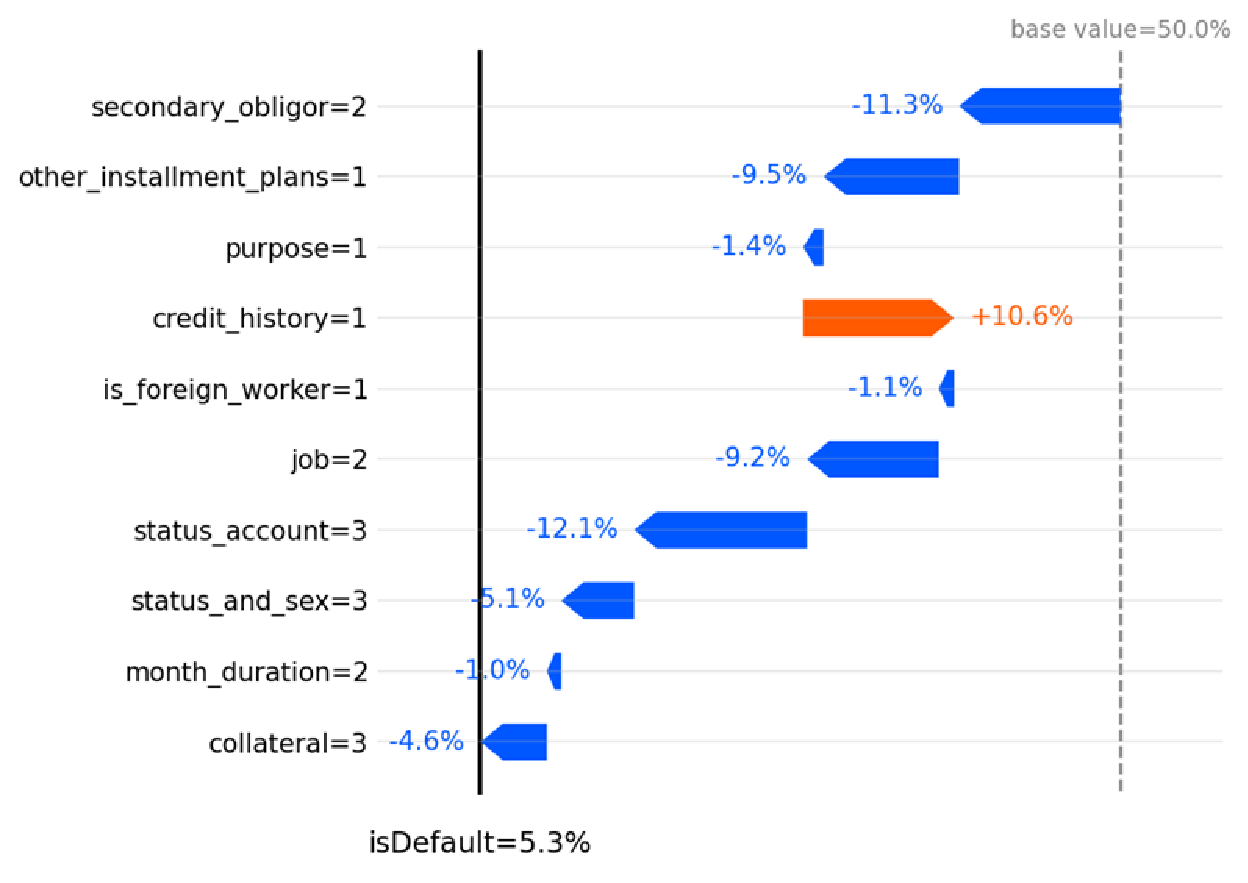
\includegraphics[width=\textwidth]{image/limeshap/ger_lime_2.pdf}
    \caption{Mạng Bayes}
    \label{fig:ger_waterfall}
\end{subfigure}
\vspace{0.8em}
\begin{subfigure}[b]{1.1\textwidth}
    \centering
    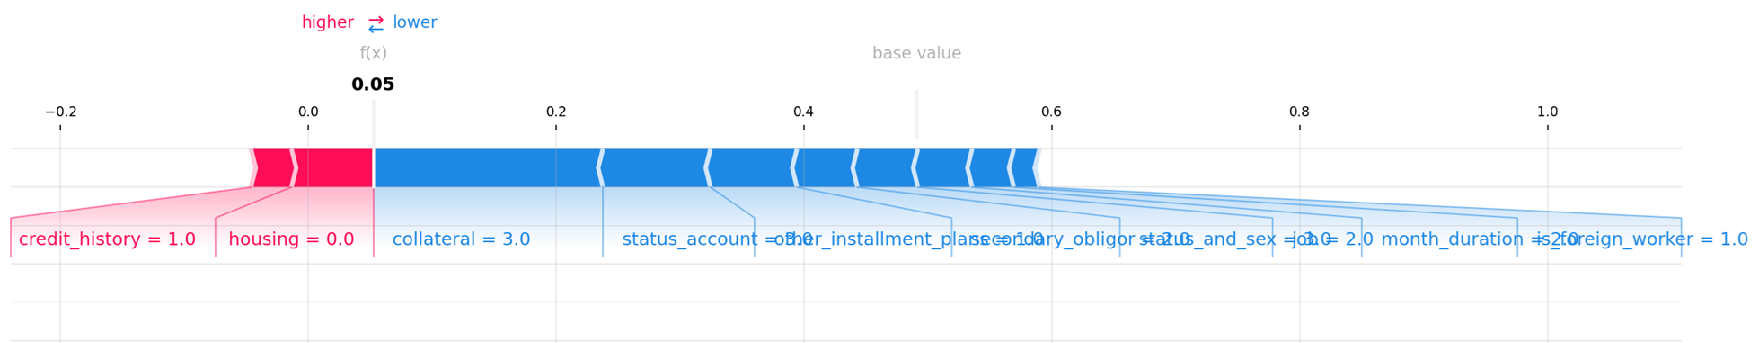
\includegraphics[width=\textwidth]{image/limeshap/ger_shap.pdf}
    \caption{SHAP}
    \label{fig:ger_shap}
\end{subfigure}
\caption{So sánh ba phương pháp giải thích cục bộ cho một hồ sơ khách hàng ngẫu nhiên --- German Credit}
\label{fig:explain_german}
\end{figure}

\begin{figure}[htbp]
\centering
{\small \textbf{Xác suất dự đoán}: Is default ~=~0.0338, No default~=~0.9662 }\\[0.3em]

\vspace{0.8em}
\begin{subfigure}[b]{0.9\textwidth}
    \centering
    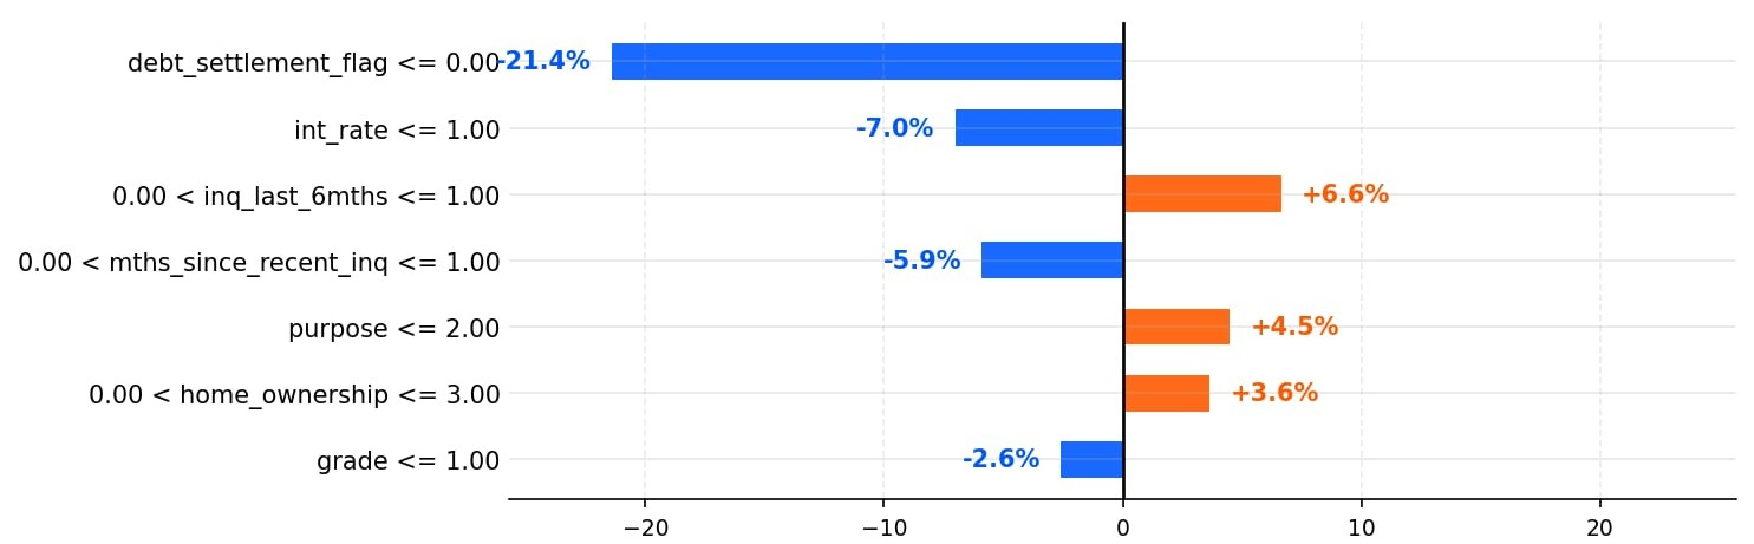
\includegraphics[width=\textwidth]{image/limeshap/lend_lime_1.pdf}
    \caption{LIME}
    \label{fig:lend_lime}
\end{subfigure}
\vspace{0.8em}
\begin{subfigure}[b]{0.8\textwidth}
    \centering
    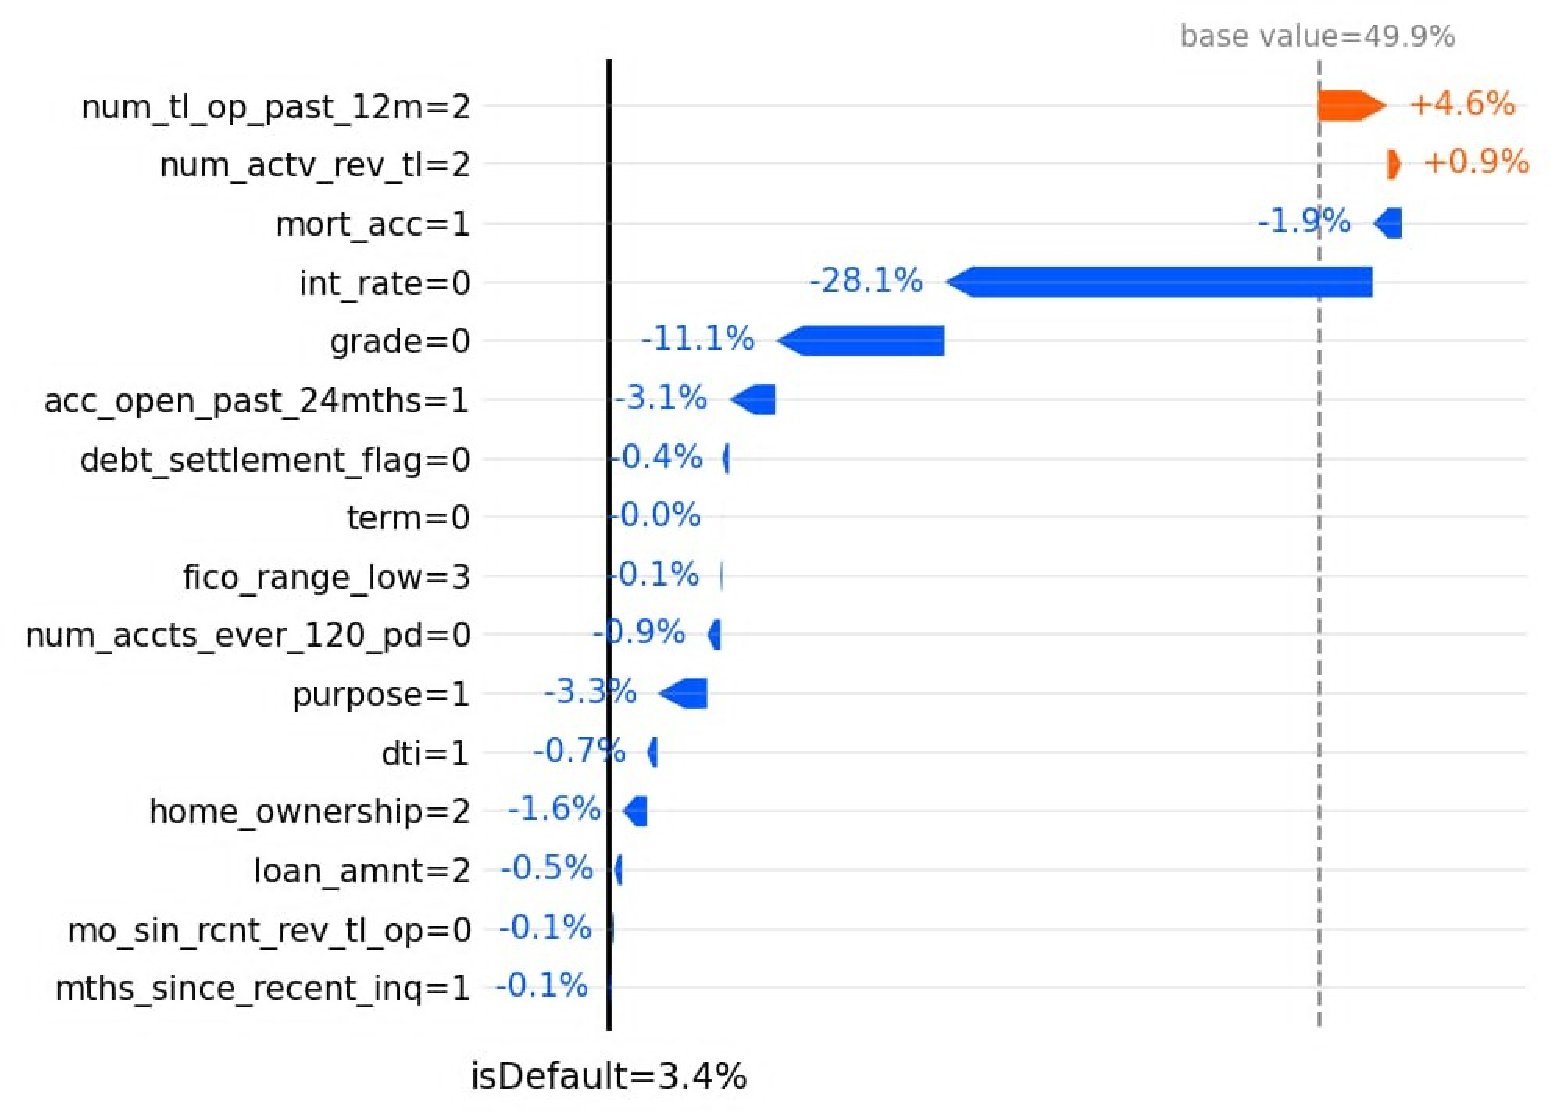
\includegraphics[width=\textwidth]{image/limeshap/lend_lime_2.pdf}
    \caption{Mạng Bayes}
    \label{fig:lend_waterfall}
\end{subfigure}
\vspace{0.8em}
\begin{subfigure}[b]{1.1\textwidth}
    \centering
    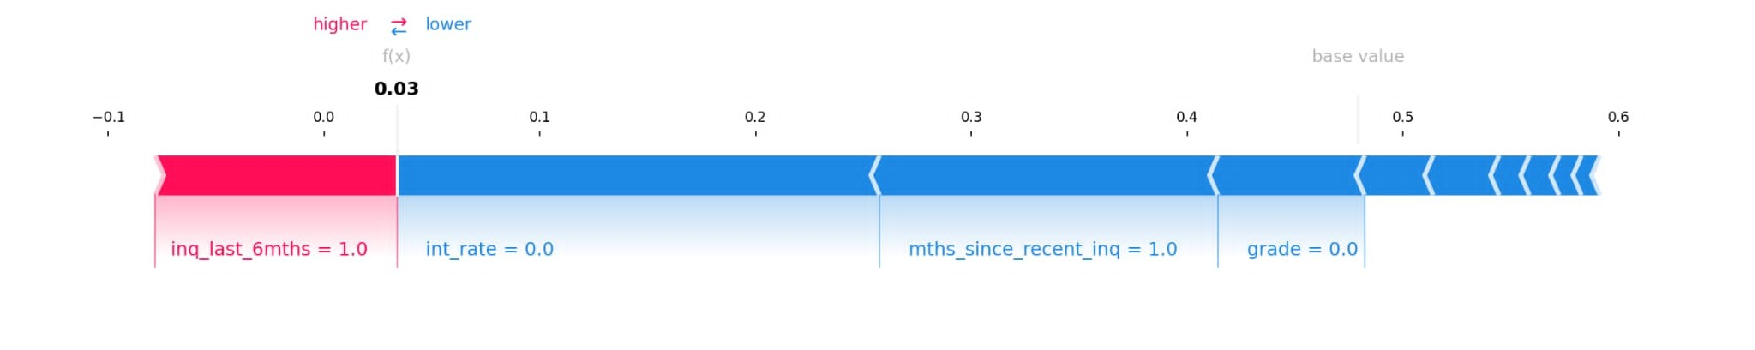
\includegraphics[width=\textwidth,
        height=0.18\textheight,
        trim=1cm 1cm 0cm 0cm,
        clip]{image/limeshap/lend_shap.pdf}
    \caption{SHAP}
    \label{fig:lend_shap}
\end{subfigure}
\caption{So sánh ba phương pháp giải thích cục bộ cho một hồ sơ khách hàng ngẫu nhiên --- Lending Club}
\label{fig:explain_lendingclub}
\end{figure}

\FloatBarrier

%\input{project/8_}
\section{Tổng kết}

\subsection{Kết quả của khóa luận}

\noindent
Kết quả thực nghiệm trên ba bộ dữ liệu khẳng định mô hình BN\_Pro kết hợp học cấu trúc bằng BIC-Tabu Search với ràng buộc tri thức chuyên gia, học tham số bằng MLE, suy diễn chính xác bằng VE, và bộ công cụ diễn giải đầy đủ (sensitivity, forward/backward inference, Individual Analysis, what-if) không chỉ cạnh tranh được về độ chính xác dự báo với các mô hình học máy hiện đại trên các bộ dữ liệu quy mô vừa và nhỏ (vượt trội tuyệt đối trên Australian Credit), mà còn cung cấp khả năng diễn giải nhân quả tường minh mà các mô hình khép kín như XGBoost hay Stacking Ensemble không có sẵn.

Hiệu năng dự báo của BN biến thiên mạnh theo quy mô và độ phức tạp dữ liệu: ROC-AUC tăng từ 0.6910 (Lending Club, 27 biến) lên 0.7667 (German Credit, 15 biến) và đạt đỉnh 0.9220 (Australian Credit, 8 biến), có xu hướng ngược chiều với số lượng đặc trưng đầu vào.


So với các mô hình học máy hiện đại, BN không phải lúc nào cũng là lựa chọn tối ưu về độ chính xác thuần túy: trên dữ liệu lớn nhiều chiều, các mô hình tổ hợp cây (XGBoost, Random Forest) vượt trội hơn; trên dữ liệu nhỏ, ít chiều, BN có thể vượt qua toàn bộ các mô hình đối chứng kể cả Stacking Ensemble.


Phân tích DCA xác nhận BN mang lại lợi ích ròng dương và vượt trội hơn các chiến lược biên (Treat All / Treat None) trong vùng ngưỡng xác suất hợp lý trên cả ba bộ dữ liệu, khẳng định giá trị ứng dụng thực tiễn dù chỉ số AUC tuyệt đối có thể thấp hơn các mô hình đối chứng ở một số trường hợp.

Ưu thế nổi bật và khác biệt của BN so với các mô hình đối chứng là khả năng diễn giải tường minh thông qua cấu trúc đồ thị nhân quả và phân tích độ nhạy xác suất hậu nghiệm — một năng lực mà các mô hình khép kín (Random Forest, XGBoost, mạng nơ-ron) không có sẵn, đòi hỏi phải bổ sung các công cụ diễn giải hậu kỳ riêng biệt (như SHAP, LIME).


Quá trình tối ưu hóa cấu trúc bằng Tabu Search với 50 lần chạy độc lập cho thấy độ ổn định nghịch biến với số lượng biến: bộ dữ liệu càng nhỏ, không gian cấu trúc càng hẹp, kết quả hội tụ giữa các lần chạy càng nhất quán.


\subsection{Hạn chế và hướng phát triển}
Hạn chế lớn nhất quan sát được đối với mô hình BN trên bộ dữ liệu quy mô lớn (Lending Club) là khoảng cách hiệu năng giữa train và test (0.7944 so với 0.6910), phản ánh rủi ro overfitting cấu trúc khi số lượng biến và số cạnh đồ thị tăng cao. Việc rời rạc hóa biến liên tục bằng K-means cũng là một nguồn mất thông tin tiềm tàng, đặc biệt ảnh hưởng đến các biến tài chính có phân phối liên tục đa dạng như annual\_inc, dti, revol\_util. 

Kết quả trên Lending Club cũng bộc lộ giới hạn về khả năng mở rộng (scalability) của suy diễn chính xác khi số đặc trưng và độ phức tạp cấu trúc DAG tăng cao, cũng như hiện tượng CPT thưa dẫn tới xác suất cực đoan khi suy luận tiến chỉ dựa trên evidence hẹp. Đây là cơ sở thực nghiệm để đề xuất các hướng cải tiến: giới hạn chặt hơn max\_indegree, áp dụng suy diễn xấp xỉ (approximate inference) thay cho khử biến trên các bộ dữ liệu quy mô lớn, hoặc khai thác BN như thành phần diễn giải bên trong kiến trúc các mô hình kết hợp thay vì một mô hình dự báo độc lập hoàn toàn.


Hướng phát triển trong tương lai bao gồm: (i) áp dụng các kỹ thuật regularization mạnh hơn trong bước học cấu trúc (ví dụ giảm max\_indegree hoặc áp đặt expert\_knowledge/forbidden\_edges chặt chẽ hơn); (ii) thử nghiệm các phương pháp rời rạc hóa thích nghi (adaptive binning) thay cho K-means cố định; (iii) mở rộng so sánh với các biến thể Mạng Bayes liên tục (Gaussian Bayesian Network, Hybrid BN) để giảm thiểu mất mát thông tin do rời rạc hóa, đặc biệt phù hợp với các bộ dữ liệu quy mô lớn như Lending Club.

\subsection{Kết luận}
\noindent
Nghiên cứu xuất phát từ một câu hỏi thực tiễn có tính cấp thiết cao trong lĩnh vực tài chính ngân hàng hiện đại: liệu có thể xây dựng một mô hình dự báo rủi ro tín dụng vừa đạt hiệu năng phân loại cạnh tranh, vừa cung cấp giải thích nhân quả có chiều sâu đủ để phục vụ thực tiễn thẩm định và quản lý rủi ro thay vì phải chọn một trong hai? Câu trả lời mà nghiên cứu này đưa ra được kiểm chứng bởi bằng chứng thực nghiệm trên ba bộ dữ liệu độc lập là có, nhưng có điều kiện. Điều kiện đó là chất lượng toàn bộ pipeline chuẩn bị dữ liệu trước khi đưa vào mô hình sinh: lọc đặc trưng phù hợp, kiểm soát rò rỉ thông tin, và chiến lược rời rạc hóa tương thích với phân phối từng biến.


Bằng chứng cho luận điểm này được rút ra trực tiếp từ kết quả thực nghiệm. Trên bộ Australian Credit với pipeline chuẩn bị dữ liệu đạt chất lượng đồng đều nhất với chỉ 8 đặc trưng đã được lọc kỹ và rời rạc hóa nhất quán, BN đạt AUC-ROC 0.9220 trên tập test, xếp hạng 1/6, vượt qua cả Stacking Ensemble (0.9035), Logistic Regression (0.9052), Random Forest (0.9046), XGBoost (0.8919) lẫn KNN (0.8415). Đáng chú ý hơn, BN đạt điều này với khoảng cách overfitting thấp nhất trong nhóm: AUC train là 0.9278, tức khoảng cách train–test chỉ 0.0058, trong khi XGBoost là 0.0852 (train 0.9771 so với test 0.8919), KNN lên tới 0.1555 (train 0.9970 so với test 0.8415), và ngay cả Stacking Ensemble cũng có khoảng cách 0.0570 (train 0.9605 so với test 0.9035). Điều này cho thấy BN khi được cấp dữ liệu đầu vào phù hợp với giả định rời rạc của nó, không thua kém các mô hình ensemble về AUC và vượt trội đáng kể về độ ổn định tổng quát hóa (generalization stability), một đặc tính then chốt trong bối cảnh triển khai thực tiễn tín dụng nơi phân phối dữ liệu luôn dịch chuyển theo thời gian.


Đóng góp cốt lõi vượt ra ngoài con số AUC là khung suy luận bốn chiều In\_Pro, mang lại loại giá trị mà không mô hình phân biệt nào có thể cung cấp từ cùng một mô hình duy nhất: định lượng độ nhạy từng biến trong Markov Blanket, trả lời câu hỏi chẩn đoán ngược về đặc điểm của khách hàng đã vỡ nợ, giải thích xác suất vỡ nợ ở cấp độ từng hồ sơ cụ thể, và định lượng tác động can thiệp khi thay đổi từng yếu tố rủi ro. Ba phép phân tích độc lập sensitivity, likelihood ratio, và individual contribution hội tụ nhất quán về cùng tập biến chi phối rủi ro, xác nhận cấu trúc đồ thị học được phản ánh đúng các quan hệ phụ thuộc có ý nghĩa miền thực sự trong từng bối cảnh tín dụng.

Giới hạn thực sự của mô hình sinh không phải là về hiệu năng phân loại khi dữ liệu và pipeline phù hợp, mà là về khả năng mở rộng sang không gian đặc trưng lớn và dữ liệu phi cấu trúc. Trên Lending Club với 27 đặc trưng, BN đạt AUC = 0.6910. Đây không phải thất bại trong nghiên cứu mà là kết quả hợp lý của một mô hình sinh buộc phải rời rạc hóa toàn bộ không gian đặc trưng liên tục và học cấu trúc phụ thuộc từ dữ liệu có nhiều quan hệ phi tuyến cục bộ, vốn là điều kiện để các mô hình phân biệt dựa trên cây quyết định xử lý hiệu quả hơn về mặt bản chất. Sự đánh đổi này không phủ nhận giá trị của BN, mà làm rõ vùng ứng dụng phù hợp: BN phát huy lợi thế tối đa trong bối cảnh không gian đặc trưng vừa phải, cấu trúc phụ thuộc tương đối rõ ràng, và yêu cầu giải thích nhân quả là ưu tiên hàng đầu, đây chính xác là bối cảnh của phần lớn bài toán thẩm định tín dụng thực tiễn tại các tổ chức tín dụng quy mô vừa và nhỏ.


\input{project/10_Ketluan}
\input{project/11_Insight}

\newpage

%% Phan trang sau cua luan van
\setlength{\parskip}{6pt}
\baselineskip = 15pt
\setlength{\headheight}{15pt}


%%%% References

\renewcommand{\refname}{Tài liệu tham khảo}

\nocite{*}
\bibliographystyle{plain}
\bibliography{references}
\addcontentsline{toc}{section}{Tài liệu tham khảo}
\clearpage

% %% Phụ lục
% \section*{Phụ lục}
% \phantomsection
% \addcontentsline{toc}{section}{Phụ lục}
% \input{project/12_Phuluc}

\end{document}

